% exemplo genérico de uso da classe iiufrgs.cls
% $Id: iiufrgs.tex,v 1.1.1.1 2005/01/18 23:54:42 avila Exp $
%
% This is an example file and is hereby explicitly put in the
% public domain.
%
\documentclass[pgmicro,mestrado,english]{iiufrgs}
% um tipo específico de monografia pode ser informado como parâmetro opcional:
%\documentclass[tese]{iiufrgs}
% monografias em inglês devem receber o parâmetro `english':
%\documentclass[diss,english]{iiufrgs}0
% a opção `openright' pode ser usada para forçar inícios de capítulos
% em páginas ímpares
% \documentclass[openright]{iiufrgs}
% para gerar uma versão somente-frente, basta utilizar a opção `oneside':
% \documentclass[oneside]{iiufrgs}
\usepackage[T1]{fontenc}        % pacote para conj. de caracteres correto
\usepackage[utf8]{inputenc}   % pacote para acentuação
\usepackage{graphicx}           % pacote para importar figuras
\usepackage{times}              % pacote para usar fonte Adobe Times
\usepackage{textcomp}
\usepackage{mathptmx}          % p/ usar fonte Adobe Times nas fórmulas
\usepackage{caption}
\usepackage{subcaption}
\usepackage{multirow}
\usepackage[normalem]{ulem}
\usepackage{pdfpages}
\usepackage{listings}
\usepackage{amsmath}

\usepackage{bibentry}
\nobibliography*

%\usepackage{biblatex}
%\usepackage{filecontents}
%\usepackage{natbib}
%\usepackage{bibentry}
%
% Informações gerais
%
%\addbibresource{biblio.bib}
\title{Schmitt Trigger Dimensioning Under Variability and Voltage Scaling for Minimum Energy Operation.}

\author{Moraes}{Leonardo Barlette}
% alguns documentos podem ter varios autores:
%\author{Flaumann}{Frida Gutenberg}
%\author{Flaumann}{Klaus Gutenberg}

% orientador e co-orientador são opcionais (não diga isso pra eles :))
\advisor[Prof.~Dr.]{Reis}{Ricardo}
\coadvisor[Profa.~Dra.]{Meinhardt}{Cristina}

% a data deve ser a da defesa; se nao especificada, são gerados
% mes e ano correntes
%\date{maio}{2001}

% o nome do curso pode ser redefinido (ex. para TCs)
%\course{Curso de Especialização em Cachaça}

% o local de realização do trabalho pode ser especificado (ex. para TCs)
% com o comando \location:
%\location{Itaquaquecetuba}{SP}

% itens individuais da nominata podem ser redefinidos com os comandos
% abaixo:
% \renewcommand{\nominataReit}{Prof\textsuperscript{a}.~Wrana Maria Panizzi}
% \renewcommand{\nominataReitname}{Reitora}
% \renewcommand{\nominataPRE}{Prof.~Jos{\'e} Carlos Ferraz Hennemann}
% \renewcommand{\nominataPREname}{Pr{\'o}-Reitor de Ensino}
% \renewcommand{\nominataPRAPG}{Prof\textsuperscript{a}.~Joc{\'e}lia Grazia}
% \renewcommand{\nominataPRAPGname}{Pr{\'o}-Reitora Adjunta de P{\'o}s-Gradua{\c{c}}{\~a}o}
% \renewcommand{\nominataDir}{Prof.~Philippe Olivier Alexandre Navaux}
% \renewcommand{\nominataDirname}{Diretor do Instituto de Inform{\'a}tica}
% \renewcommand{\nominataCoord}{Prof.~Carlos Alberto Heuser}
% \renewcommand{\nominataCoordname}{Coordenador do PPGC}
% \renewcommand{\nominataBibchefe}{Beatriz Regina Bastos Haro}
% \renewcommand{\nominataBibchefename}{Bibliotec{\'a}ria-chefe do Instituto de Inform{\'a}tica}
% \renewcommand{\nominataChefeINA}{Prof.~Jos{\'e} Valdeni de Lima}
% \renewcommand{\nominataChefeINAname}{Chefe do \deptINA}
% \renewcommand{\nominataChefeINT}{Prof.~Leila Ribeiro}
% \renewcommand{\nominataChefeINTname}{Chefe do \deptINT}

% A seguir são apresentados comandos específicos para alguns
% tipos de documentos.

% Relatório de Pesquisa [rp]:
% \rp{123}             % numero do rp
% \financ{CNPq, CAPES} % orgaos financiadores

% Trabalho Individual [ti]:
% \ti{1}     % numero do TI
% \ti[II]{456} % no caso de ser o segundo TI

% Trabalho de Conclusão [tc]:
% além de definir explicitamente o nome do curso (\course) e o local
% de realização (\location), é necessário redefinir a nominata,
% pois as informações necessárias dependem do curso. Ex.:
%\renewcommand{\nominata}{
%        UNIVERSIDADE FEDERAL DO RIO GRANDE DO SUL\\
%        Reitora: Prof\textsuperscript{a}.~Wrana Maria Panizzi\\
%        Pró-Reitor de Ensino: Prof.~José Carlos Ferraz Hennemann\\
%        Diretor do Instituto de Informática: Prof.~Philippe Olivier Alexandre Navaux\\
%        Coordenador do curso: Prof.~Seu Creysson\\
%        Bibliotecária-chefe do Instituto de Informática: Beatriz Regina Bastos Haro
%}

% Monografias de Especialização [espec]:
% \espec{Redes e Sistemas Distribuídos}      % nome do curso
% \coord[Profa.~Dra.]{Weber}{Taisy da Silva} % coordenador do curso
% \dept{INA}                                 % departamento relacionado

%
% palavras-chave
% iniciar todas com letras minúsculas, exceto no caso de abreviaturas
%
\keyword{formatação eletrônica de documentos}
\keyword{\LaTeX}
\keyword{ABNT}
\keyword{UFRGS}

%\addbibresource{biblio.bib}

%
% inicio do documento
%
\begin{document}

% folha de rosto
% às vezes é necessário redefinir algum comando logo antes de produzir
% a folha de rosto:
% \renewcommand{\coordname}{Coordenadora do Curso}
\maketitle

% dedicatoria
% \clearpage
% \begin{flushright}
% \mbox{}\vfill
% {\sffamily\itshape
% ``If I have seen farther than others,\\
% it is because I stood on the shoulders of giants.''\\}
% --- \textsc{Sir~Isaac Newton}
% \end{flushright}

% agradecimentos
% \chapter*{Agradecimentos}
% Agradeço ao \LaTeX\ por não ter vírus de macro\ldots

\newpage
% sumario
\tableofcontents

% lista de abreviaturas e siglas
% o parametro deve ser a abreviatura mais longa
\begin{listofabbrv}{SPMD}
        \item[IoT] Internet of Things
        \item[CMOS] Complementary Metal Oxide Semiconductor
        \item[ULP] Ultra Low Power
        \item[FinFET] Fin Field Effect Transistor
        \item[SCE] Short Channel Effect
        \item[RDF] Random Dopant Fluctuation
        \item[ST] Schmitt Trigger
        \item[FA] Full Adder
        \item[$V_T$] Threshold Voltage
        \item[NBTI] Negative Bias Temperature Instability
        \item[HCI] Hot Carrier Injection
        \item[CMP] Chemical-Mechanical Polishing
        \item[LER] Line-Edge Roughness
        \item[WF] Work Function
        \item[FET] Field Effect Transistor
        \item[MOSFET] Metal Oxide Semiconductor Field Effect Transistor
        \item[PVT] Process Voltage and Temperature
        \item[WID] Within-Die
        \item[SIMD] Single Instruction Multiple Data
        \item[PDP] Power Delay Product
        \item[TGA] Transmission Gate Adder
        \item[TFA] Transmission Function Adder
        \item[CPL] Complementary Pass Transistor Logic
        \item[CNFET] Carbon Nanotube Field Effect Transistor
        \item[FDSOI] Fully Depleted Silicon On Insulator
        \item[OTS] Optimal Transistor Sizing
        \item[$L$] Gate Length
        \item[$W_{FIN}$] Fin Width
        \item[$H_{FIN}$] Fin Height
        \item[$T_{OX}$] Oxide Thickness
        \item[SOI] Silicon On Insulator
        \item[WFF] Work Function Fluctuation
        \item[SRAM] Static Random Access Memory
        \item[GOBD] Gate Oxide Break Down
        \item[ECC] Error Correcting Code
        \item[SNM] Static Noise Margin
        \item[UDSM] Ultra-Deep Sub-Micron
        \item[VTC] Voltage Transfer Curve
        \item[DRC] Design Rule Checking
        \item[LVS] Layout Versus Schematic
        \item[EDA] Electronic Design Automation
        \item[PDK] Process Design Kit
        \item[ASAP] Arizona State Predictive PDK
        \item[FEOL] Front End Of Line
        \item[MOL] Middle End Of Line
        \item[BEOL] Back End Of Line
        \item[SDT] Source-Drain Trench
        \item[LIG] Local-Interconnect Gate
        \item[LISD] Local-Interconnect Source-Drain
        \item[V0] Via 0
        \item[M1] Metal 1
        \item[M2] Metal 2
        \item[MC] Monte Carlo
        \item[EDP] Energy Deviation Product
        \item[TIST] Triple-Inverter ST
        \item[SIG] Stacked-Inverter Gate
\end{listofabbrv}

% idem para a lista de símbolos
%\begin{listofsymbols}{$\alpha\beta\pi\omega$}
%       \item[$\sum{\frac{a}{b}}$] Somatório do produtório
%       \item[$\alpha\beta\pi\omega$] Fator de inconstância do resultado
%\end{listofsymbols}

% lista de figuras
\listoffigures

% lista de tabelas
%\listoftables

% resumo na língua do documento
\begin{abstract}
{The emergence of IoT alongside with the increased process variability impact in modern technology nodes, is the main reason to control variability impact over metrics. Given the large set of IoT devices working in battery-oriented environments, energy consumption should be minimal and the operation regime reliable. Schmitt Trigger inverters are traditionally used for noise immunity enhancement, and have been recently applied to mitigate radiation effects and process variability impact. However, Schmitt Trigger operation at the nominal voltage introduces high degradation on power consumption. Thus, this work main contribution is to identification of the relationship between transistor sizing, supply voltage, energy, and process variability robustness to get a minimal energy consumption circuit while keeping robustness. The results are extracted from 7-nm FinFET Schmitt Trigger layouts under different levels of process variability, supply voltages, and sizing. Also, a maximum frequency scaling under a failure threshold was performed. On average, the supply voltage decreases in layouts with a smaller number of fins, while maintaining acceptable robustness in high variability scenarios. Exploring voltage and transistor sizing made possible a reduction of about 24.84\% of power consumption. }
\end{abstract}

% resumo na outra língua
% como parametros devem ser passados o titulo e as palavras-chave
% na outra língua, separadas por vírgulas
\begin{englishabstract}
{
Dimensionamento de Schmitt Trigger Sob Influência de Variabilidade e Escalonamento da Tensão de Alimentação para Operação com Consumo Mínimo de Energia
}
{
O surgimento da Internet das Coisas juntamente com o aumento do impacto da variabilidade de processo nos nós modernos de tecnologia é o principal motivo para controlar o impacto da variabilidade sobre as métricas. Dado o grande conjunto de dispositivos envolvidos na Internet das Coisas que funcionam em ambientes orientados para baterias, o consumo de energia dever ser o mínimo possível e o regime de operação confiável. Os inversores Schmitt Trigger na tensão nominal introduzem uma alta degradação no consumo de energia. Assim, a principal contribuição deste trabalho é a identificação da relação entre o dimensionamento do transistor, a tensão de alimentação, a energia e a robustez à variabilidade de processo para obter um circuito com consumo mínimo de energia, mantendo a robustez. Os resultados são extraídos de leiautes FinFET Schmitt Trigger de 7-nm sob diferentes níveis de variabilidade de processo, tensões de alimentação e dimensionamento. Além disso, foi executada uma calibração da frequência máxima sob um limiar de falha. Em média, a tensão de alimentação diminui em leiautes com um número menor de fins, mantendo robustez aceitável em cenários de alta variabilidade. A exploração da calibragem da tensão de alimentação e dimensionamento do transistor possibilitou uma redução de até 24.84\% do consumo de energia.
}
\end{englishabstract}

\chapter{Introduction}
%\section{Internet of Things / Ultra Low Power Applications}
    The Internet of Things (IoT) has emerged to be one of the major mainstream trends, shaping technology development and the industry. The IoT concept englobes the shift from an internet which used to interconnect end-user devices to, nowadays, interconnect physical objects that communicate with each other and/or with humans \cite{miorandi2012internet}. The IoT rise alongside battery technology improvements has provided us with portable, powerful and useful equipment for our daily routine, with wireless communication making information available anytime and anywhere \cite{manoli2010energy}.

    IoT devices have been applied in many different scenarios, from improving building maintenance, to sensoring remote areas for environmental observation and even in cars, for better safety and comfort. However, while many devices have to be connected to the power grid, sensor nodes are expected to be self-sufficient. Additionally, batteries, the traditional means of powering self-sufficient systems, need to be replaced and/or charged, which means maintenance must be frequently performed \cite{bleitner2018comparison}. Given that, energy harvesting in combination with rechargeable batteries has become a viable way to alleviate the power source and consumption dilemma \cite{manoli2010energy}.

    Energy harvesting makes use of readily available power sources in the vicinity as for example motion or vibration induced kinetic energy, solar and electromagnetic or temperature gradients. A number of viable solutions are already present on the market, like self powered wireless light switches and electro-magnetic generators, which converts vibrations available in industrial plants for powering wireless monitoring sensors \cite{manoli2010energy} \cite{bleitner2018comparison}. Although, regardless of the sensors power supply, it will be always restricted by its power budget, with devices which are able to perform their functionality under heavy power constraints being essential for IoT. In traditional Complementary Metal Oxide Semiconductor (CMOS) circuit design aimed at Ultra Low Power (ULP) applications, the ideal circuit is the one that performs a given task or functionality while consuming the least amount of energy. Such circuits are achieved under transistor sizing and supply voltage tuning, and are technology and application-dependent.

    Nevertheless, the performance of a system operating in its minimum energy per operation point may exceed the power budget of a given application. For example, with an application such as presented in \cite{fojtik2013millimeter}, where the device is only active once per hour, with 80\% of its power consumption being due to standby power. In such a case, the minimization of energy-per-operation seems to be suboptimal in comparison to a idle power minimization kind-of solution. The minimization of supply voltage brings advantage for certain energy harvesting approaches such as thermo-electric. Such harvesting technique can result in DC voltage levels from tens to even hundreds of milivolts \cite{khan2014flexible}.

    Technology scaling is a major factor in the ascendance of IoT, providing higher transistor densities and voltage scaling due to the miniaturization of gate dimensions, internal capacitances and resistances. These two parallel events contributed for the emergence of IoT \cite{islam:10}. Alongside, with the advance of transistor technology, new challenges were introduced due to the scale down, as aging effects, high power consumption due to leakage current and an increase in the sensibility to transient faults due to radiation and variability \cite{abbas:15}.

    The Fin Field Effect Transistor (FinFET) transistor technology has been adopted to overcome those challenges. FinFET devices present superior channel control due to the reduced Short Channel Effects (SCE) and low (if none) Random Dopant Fluctuation (RDF) effect due to the fully depleted channel \cite{farkhani2014comparative}. Although, at deep technology nodes, variability is one of the most challenging factors, including on FinFET devices. Variability introduces behavior changing geometrical inconsistencies to the final manufactured product. Such variations influence the circuits metrics, hastening its degradation and deviating from its correct operation regime \cite{abbas:15} \cite{nassif:08}.

    Given the energy constraints of IoT applications and the variability impact on recent nodes, the Schmitt Trigger (ST) circuit has been pointed as an alternative. The classical ST has been employed as a key element for several ULP circuits \cite{kulkarni2007160, hays201262, melek:17, lotze2017ultra} and for variability mitigation, mainly attenuating the deviation on the power consumption. ST was applied replacing internal inverters of full adders (FAs) in \cite{dokania2015circuit} where spreads in major metrics were successfully limited. Also, the same experiment was executed at electrical and layout levels considering FinFET technology, and showed a considerable decrease in overall variability impact on metrics \cite{toledo2018pros,moraes2018evaluation}. However, with a considerable increase in delay and power consumption. In addition to previous work, this work will present further analysis related to the Schmitt Trigger technique applied on FAs, with the classical ST being considered, apart from the original analysis with only a low power ST. Furthermore, a considerable part of this work consists of evaluations about the behavior of the classical ST, the Stacked Inverter Gate (SIG) \cite{bose2018stacked} and Triple Inverter Schmitt Trigger (TI-ST) \cite{luo2017sub} over several scenarios of sizing, supply voltage, and process variability level, in order to identify the most apropriate set of characteristics for each design.

    This work is divided into five further sections: Variability Effects and Mitigation Techniques, where a theoretical foundation about variability is laid with several related works about mitigating its impact, FinFET Technology and Variability Impact, will show the characteristics of FinFET devices and how process variability presents itself in the device. A section about the considered circuits will explain their functionality and applications. Objectives section, will lay the main objectives based on the beforehand laid concepts. The Methodology section will explain the experimental setup which will be employed to generate the results. A Results section is present, showing some preliminary results and analysis. Lastly, there are a Conclusions and Future Works sections.

\chapter{Variability Effects and Mitigation Techniques}

As process technology scaling advanced, decreasing the transistor dimensions, the ratio between device size and atom-size have been decreasing as well. Multiple techniques have been developed to reduce the loss of precision due to the manufacturing process at different end-of-lines. However, as the quantum-mechanical limit approaches, manufacturing-induced imprecision impact rises \cite{asenov1999random}.

Variability consists of characteristic deviations, internal or external to the circuit, which can determine its operational features and can be divided by three types concerning its sources:

\textit{Environmental Factors or use-induced variation} is mostly external to the circuit, it englobes variations in the power supply voltage and temperature. Voltage drops mainly occur due to abrupt changes in the switching activity, inducing large current transients in the system both locally or globally across the due. Local temperature within the die can cause variations in the device mobility and threshold voltages ($V_T$), and wire resistance. It is highly design dependent with timing constants similar to clock frequency \cite{nassif:08} \cite{bernstein2006high}.

\textit{Reliability Factors} are related to the aging process of the circuit. Circuit aging is defined by numerous phenomena: Negative Bias Temperature Instability (NBTI) which mines the performance of p-channel due to the weakening of Si-H bonds in the oxide generating of interface states and trapping positive charges while the device is operating \cite{wang2008statistical}, electromigration due to high enough current densities causing the gradual movement of metal ions due to the electron-ion momentum transfer \cite{young1994failure}, time dependent dielectric breakdown due to current flowing through gate oxides \cite{lombardo2005dielectric} and Hot Carrier Injection (HCI) trapping electrons on oxide which degrades n-MOSFET on-current \cite{takeda1983empirical} \cite{nassif:08} \cite{bernstein2006high}.

\textit{Physical Factors} are caused by the manufacturing process, consequence of imprecisions in the manufacturing process, resulting in characteristic deviations of active and passive components. Those variations can be:

    \begin{itemize}
        \item Systematic or extrinsic: is related to unintentional imprecisions in the manufacturing process, not associated with fundamental atom-related problems. Extrinsic variability can present itself in multiple ways, from different lots, from different wafers within a lot, across wafers and even from chip to chip. The main contributor for extrinsic variation is the chip to chip variability, with its sources being both by-wafer and by-reticle process steps. By-wafer variability is caused by three manufacturing steps: rapid thermal anneal - with a uneven temperature distribution across the wafer, photoresist development and etching and by-reticle variability can contribute due to changes in the focus as the mask is stepped across the wafer in the photolithography process. The focus can suffer deviations due to exposure tool lens astigmatisms or by wafer nonplanarity. Additionally, the within-chip variability can be divided into two types. The similar-structure variability, consists of across-wafer and across-reticle variations that each chip ends up intercepting, and the dissimilar-structure which consists of variations caused by processing steps that differ by structure and layout variations of structure (difference of orientation for the same structures in the layout as well as variations in polygon densities) \cite{bernstein2006high}.

        \item Design dependent: variations related to the placement can results in changes in the electrical parameters of active and passive devices. The sources of such type of variability include manufacturing related deviations. Manufacturing variability may be systematic, having a well-known relationship between design or layout and the final electrical parameters values. Chemical-Mechanical Polishing (CMP) relationship between the thickness of the metal and the layout feature density \cite{stine1997analysis}. The main difference between systematic and random variability is the way it is treated at design time. Systematic variability can be modeled and anticipated, allowing the designer to tune the layout or timing for mitigation. Random variations, however, require the designer to add time margins in order to guard against the worst timing possible \cite{nassif1998within}.

        \item Random or intrinsic: consists of atomic-level deviations between devices (even when they are identical in layout and geometry). These deviations appear in dopant profiles, thickness variations, and Line-Edge Roughness (LER). Dopant fluctuations are the main cause to $V_T$ variations \cite{asenov2003simulation}, with the removal of doping from the channel contributing for the $V_T$ variation reduction, introducing the necessity to set the $V_T$ by gate-metal Work Function (WF) or by biased back gate \cite{frank2001device,wong1999nanoscale}. Fluctuations in doping levels and device features cause variations in the source/drain regions, which affects the overlap capacitance and the source resistance \cite{frank2000simulation}. LER arises from variations in the total number of incident photons during lithography. Such roughness introduction into the polygons geometry may determine the effective gate width as one moves along the x axis of a Field Effect Transistor (FET) \cite{brunner2003optical}.
        Another source of intrinsic device variability rises from the atomic-scale oxide thickness variation. It can introduce variations in the $V_T$ \cite{asenov2003simulation}, in the oxide tunneling current, and may cause mobility degradation due to the potential variation across the Metal Oxide Semiconductor FET (MOSFET) channel \cite{bernstein2006high}. Fig. \ref{fig:transAbs}, depicts the transistor intrinsic variability.
    \end{itemize}

    \begin{figure} [H]
        \centering
        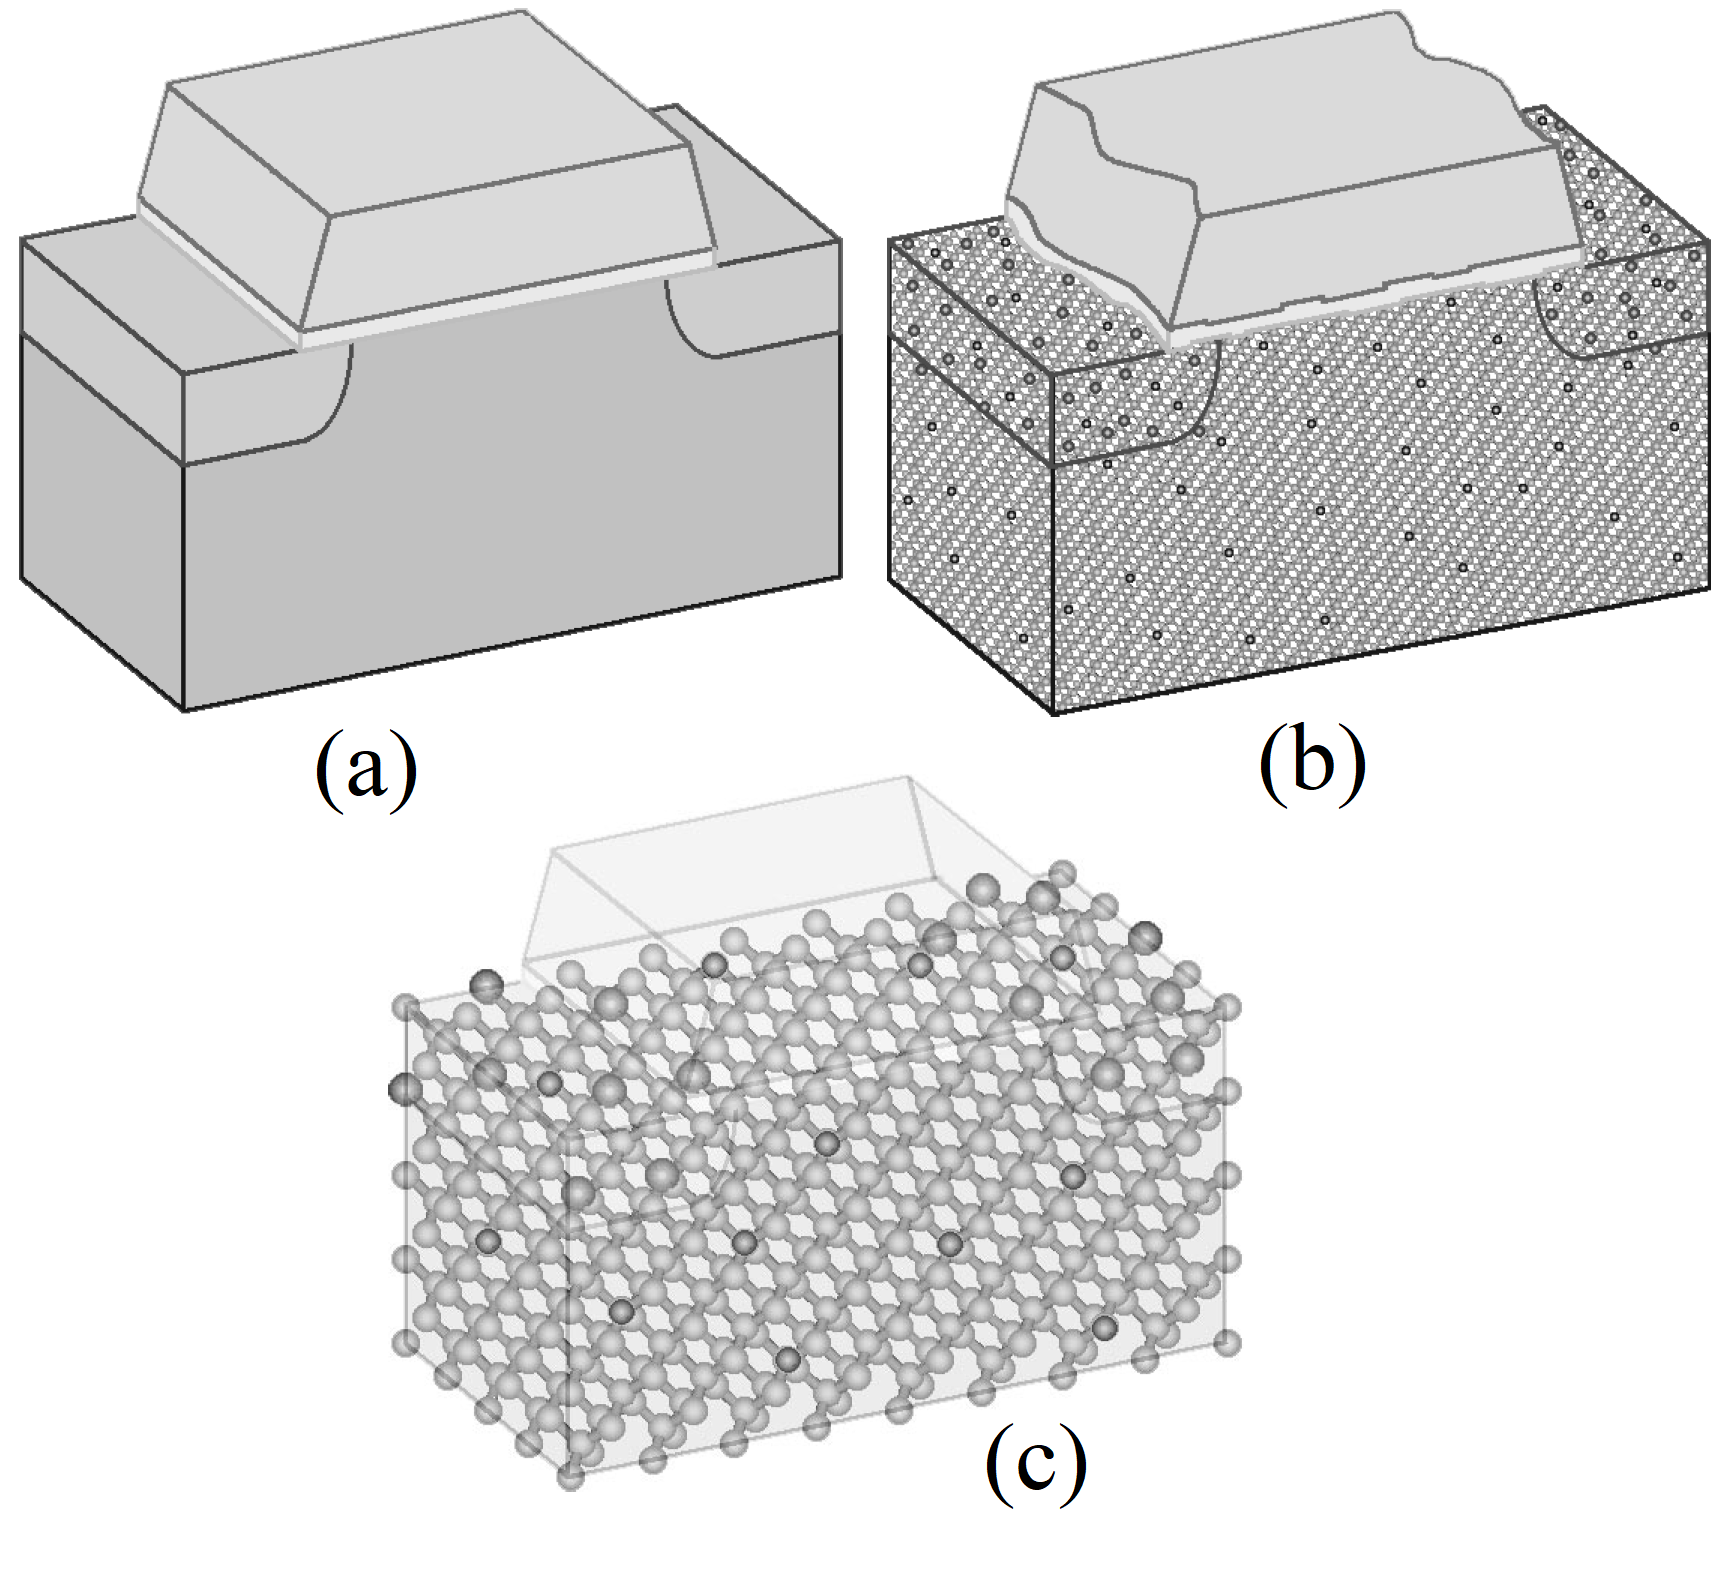
\includegraphics[width=0.65\textwidth, trim={0 0 0 0},clip]{transistorVariability.png}
        \caption{Levels of abstraction from a ideal transistor concept towards a realistic and "atomistic" device concept. (a) Depicts a the current approach of semiconductor device simulation, with continuous dopant charge and smooth boundaries. (b) Depicts a 20-nm MOSFET, with less than 50 Si atoms along the channel. RDF, interface roughness and LER introduce considerable intrinsic parameter fluctuation. (c) Depicts a 4-nm MOSFET, with less than 10 Si atoms along the channel. }
        \label{fig:transAbs}
        \legend{Source: \citet{asenov2003simulation}}
    \end{figure}

% Please add the following required packages to your document preamble:
% \usepackage{graphicx}
\begin{table}[H]
\centering
\caption{Impact of variability on performance and power.}
\label{tab:abbastech1}
\resizebox{\textwidth}{!}{%
\begin{tabular}{lcccc}
\hline
\textbf{Property} & \textbf{Ease of measuring} & \textbf{Variability} & \textbf{Effects of variability} & \textbf{Effect of missing specification} \\ \hline
\textbf{Performance} & Medium & Medium: up to 60\% & L, W, R, C, $V_T$, \(\mu\) & Slower product, yield, timing error \\ \hline
\textbf{Leakage Power} & Easy & Large: up to 148\% & L,  $V_T$, \(\mu\), $t_{ox}$ & Shorter battery life, yield, heat \\ \hline
\textbf{Dynamic Power} & Difficult & Workload dependent & C, \(\alpha\) & Shorter battery life, heat \\ \hline
\end{tabular}%
}
\legend{Source: \citet{rahimi2016variability}}
\end{table}

Table \ref{tab:abbastech1} illustrates the variations impact on performance and power. As a way to handle timing errors due to variations in the path delay, circuit designers commonly add safety timing margins to the voltage and/or the clock frequency (guardband). Such practice leads to overly conservative designs due to the guardband overlapping and accumulation in the ever increasing multi-corner analysis \cite{austin2005opportunities}.


In \cite{jeong2009impact} the impact of each individual variability source: Process, Voltage and Temperature (PVT) is quantified concerning a standard inverter cell through SPICE simulations. A 1.8x delay variations was observed, with 1.46x, 1.25x and 0.97x coming from the process, voltage and temperature variations, respectively. Under the same operation conditions smaller supply voltages for a 80-core Intel processor, it was observed a normalized deviation of 5.93\%, 6.37\% and 8.64\% for 1.2 (nominal), 0.9, and 0.8V, respectively. The lowering from 1.2 to 0.8V increases the critical path variability up to 45\% \cite{dighe2011within}.

Near-threshold operation has become a popular technique to achieve energy-efficient digital circuits. Although, operating at low voltages exacerbates the effects of delay variations \cite{jeon2012design, dreslinski2010near, rithe2011effect, kakoee2012variation, pawlowski2012530mv}.
The measurement of Within-Die (WID) delay was performed for a 45nm Single Instruction Multiple Data (SIMD) processor, showing that reducing $V_{DD}$ from 1.0 to 0.53 V increases delay variation by 6x \cite{pawlowski2012530mv}.

Given the increase in performance variation, there is the need for mitigation methods to make the design resilient to timing errors, especially for circuits at low voltage operation regimes. There are several approaches to how and when errors should be manipulated as well as their abstraction levels. Among the steps there are: Predicting and Preventing, Detecting and Correcting, and Accepting. And among the abstraction levels there are Application Algorithm, Software, Architecture and Circuit. Since this work aims to investigate variability impact at layout level, some circuit-level techniques will explained next with higher level techniques being thoroughly explained at \cite{rahimi2016variability}.

Tuning CMOS knobs consists of several approaches to tune electrical characteristics (e.g., power and delay) of circuit by interfering with the body bias supply voltage and clock frequency, for example. Forward body biasing reduces the $V_T$ (improving performance and increasing leakage power) while reverse body bias increases the $V_T$ (reducing performance and leakage power). Given so, a slow circuit block can have its performance improved upon forward body biasing while a leaky circuit can be reverse body biased. Additionally, voltage and/or the circuit's frequency can be tuned to compensate variations \cite{dighe2011within, tschanz2002adaptive, borkar2004design}.

There are topology changes employed during design time CAD optimizations in order to enhance the circuit resiliency against timing errors. Due to the general presence of clusters of critical paths in circuits some approaches focus on uncertainty-aware circuit optimizations \cite{bai2002uncertainty}. Optimization such as upsizing and downsizing of gates, use of multiple $V_T$ cells, and restructuration of the path delay distribution \cite{kahng2010slack}.

Lastly, asynchronous circuits have been proposed since there is no need for a clock signal to determine a starting time for computation. In \cite{chang2013synchronous} both versions (synchronous and  asynchronous) of 8051 microcontroller are designed. When PVT and workload variations are introduced, the synchronous version required ~4x, ~1.5x, and ~2x delay margins while the asynchronous version operated at nominal performance.

In order to mitigate variability impact, many works try to indicate the most robust design for a given type of circuit. For example, in \cite{dokania2013investigation} twelve different FA topologies are analyzed considering delay, power and Power-Delay-Product (PDP) variability. It is used a 16nm bulk CMOS technology node in SPICE simulations with PVT variability being considered and Monte Carlo simulations performed. The authors concluded that Cell A, CLRCL and Cell B FAs presented the best results for all three metrics (Delay, Power and PDP).

In \cite{ames2016investigating} the effects of PVT variability in different FA designs are investigated. The simulations are performed in HSPICE with the bulk CMOS 32nm node technology. With Transmission Gate Adder (TGA) and Transmission Function Adder (TFA) architectures showing acceptable behavior under PVT variability with the lowest power consumption sensibility amongst the tested FAs - 11x smaller in comparison with Complementary Pass Transistor Logic (CPL) FA.

In \cite{islam2011design} various popular 1-bit digital summing circuits functionality and robustness are analyzed in light of PVT variations with the best FA being simulated in Carbon Nanotube Field Effect Transistor (CNFET) technology for comparison with the bulk CMOS version. The simulations are carried at the 22nm bulk CMOS and CNFET technology node in HSPICE. Its results show that the TGA has the strongest PVT variability robustness and its CNFET version provides over 3x, 1.14x and 1.1x less propagation delay, power dissipation and energy delay product (EDP) variations, respectively. This work does not consider the total power consumption of each FA separately.

Some articles analyze the adoption of new technologies: \cite{guduri2015design} proposes a hybrid of bulk CMOS and CNFET FA at 16nm in deep subthreshold operation region for ULP applications simulated in SPICE which showed some improvement over its bulk CMOS FA counterpart achieving 5\% and 1\% improvement in power, power-delay and energy-delay products and their variability, respectively. In \cite{islam2011variability} a new subthreshold-FinFET FA is proposed and compared over multiple FAs showing huge metric improvements provided by the FinFET technology up to 2.22x improvement in power variability. It was simulated in 32nm predictive technology model on HSPICE.

It is notable that none of these works consider a layout approach for its simulations and do not address any novel general technique which can be applied to a range of different types of circuits. Although, some works introduce novel designs.

\cite{federspiel201228nm} presents reliability comparison between 28nm bulk CMOS and Fully Depleted Silicon On Insulator (FDSOI) technologies at layout level, with FDSOI showing 32\% improved performance, 40\% reduced power consumption and improved matching, with its intrinsic reliability behavior similar to 28nm bulk at the device level. \cite{alioto2007delay} presents a study about the delay variability caused by supply variations in the TGA. The experiments were performed at 90nm and 180nm bulk CMOS Technology in Spectre at layout level. It showed that lower supply voltages bring more delay variability to the circuit with the TGA presenting worse results 15\% (25\%) for the 90 nm (180 nm) in comparison to static logic.

Some works focus on evaluating techniques: In \cite{zimpeck2016finfet} three transistor sizing techniques are applied on a set of cells and their impact on variability robustness is analyzed. The simulations were performed considering a 14nm FinFET technology using HSPICE tool. The authors concluded that the Optimized Transistor Sizing (OTS) technique has the best ratio between nominal PDP and PDP under process variability.
\cite{ahmadi2017hybrid} introduces a new technique to improve the performance of digital circuits in the presence of variations. It consists of a hybrid of two former methods to prevent errors due to delay variations. The simulations were performed with a 45nm predictive technology using HSPICE and applied on ITC’99 and ISCAS’89 benchmarks circuits. The results show that the hybrid technique can tolerate process variations up to 27.3\% better than previous state-of-the-art techniques.

\chapter{FinFET Technology and Variability Impact}
    New commercial technologies have been developed for mitigation of variability impact. The Fin Field Effect Transistor (FinFET) remains as one promising new technology for variability mitigation while maintaining technology scaling. The FinFET main geometric parameters are the gate length ($L$ or $L_G$), fin width ($W_{FIN}$, $T_{FIN}$ or $T_{SI}$), fin height ($H_{FIN}$) and Oxide Thickness ($T_{OX}$). FinFET transistors can be built on a traditional bulk or on a Silicon on Insulator (SOI) substrate with a conducting channel that rises above the level of the insulator, creating a thin silicon structure, the gate, as shown in Figures \ref{mosfetvsfinfet} and \ref{bulkvssoi}. FinFET devices can be shorted-gate (3 gate nodes) or independent-gate (4 gate nodes). The shorted gate model is similar to the traditional MOSFET given that the front-gate and back-gate are connected and controlled by the gate signal. The independent gate has 4 nodes, making possible to connect the front and back gate to different voltage values.

    \begin{figure} [H]
        \centering
	    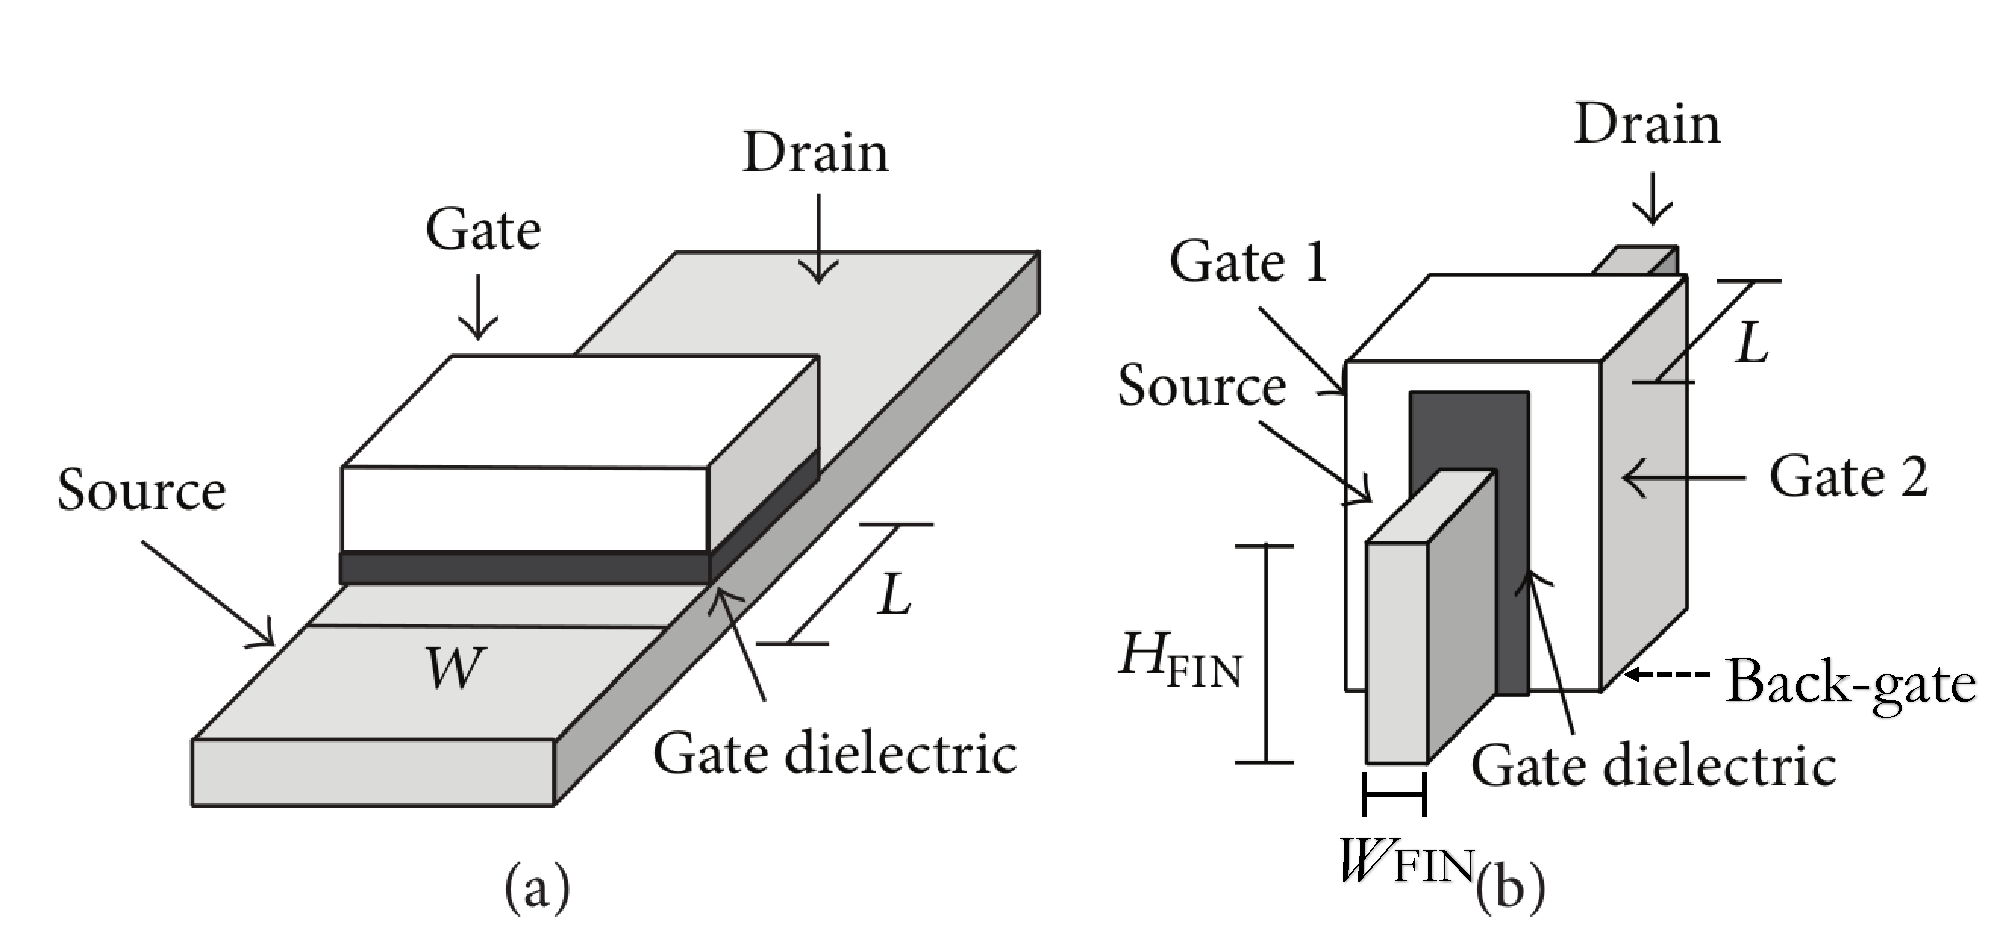
\includegraphics[width=\textwidth, trim={0 0 0 0},clip]{finfet.pdf}
        \caption{Structural comparison between (a) planar MOSFET and (b) FinFET transistors.}
        \label{mosfetvsfinfet}
        \legend{Source: \citet{bhattacharya2014finfets}}
    \end{figure}

    \begin{figure} [H]
        \centering
        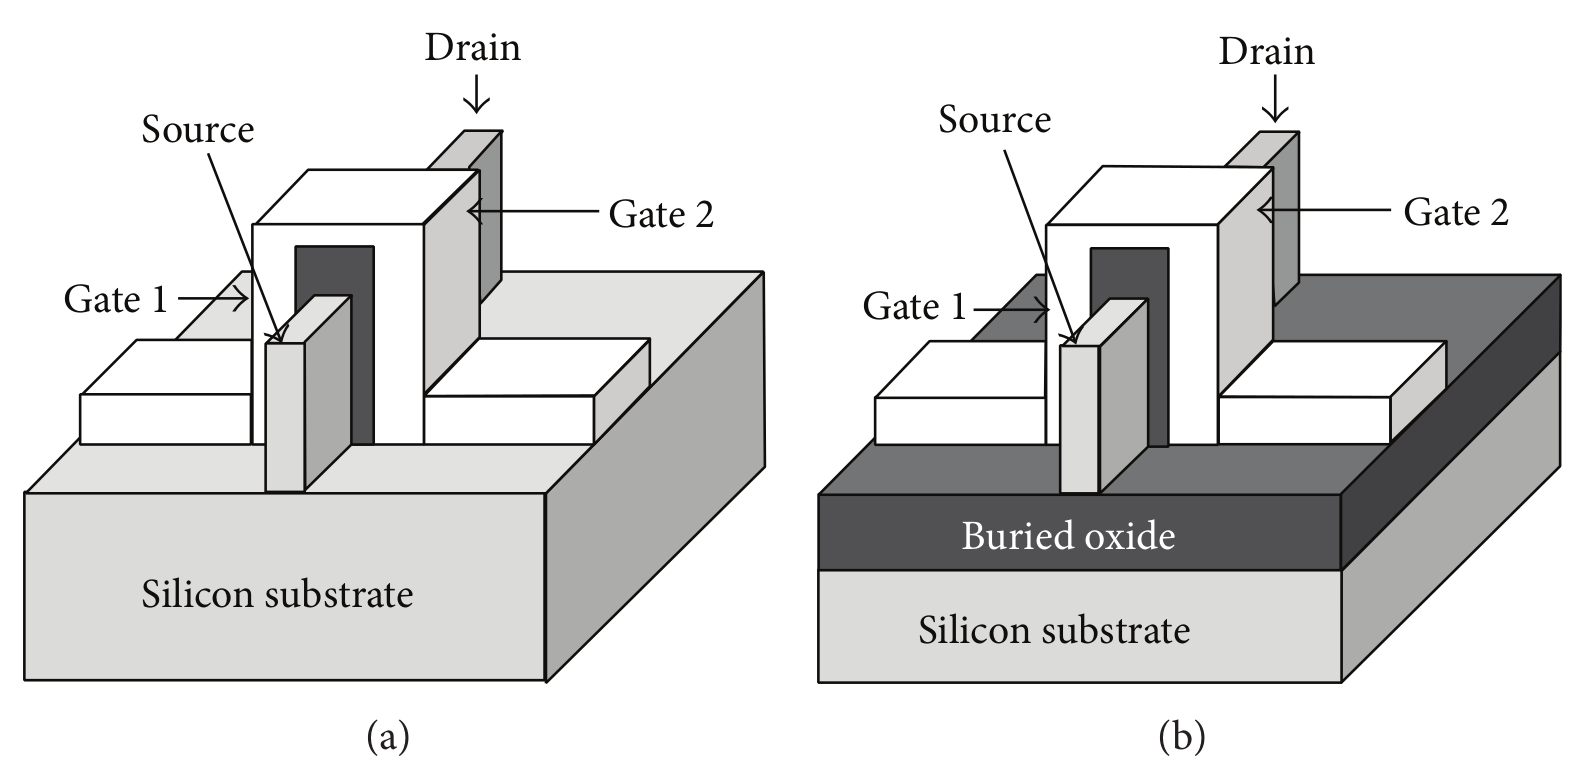
\includegraphics[width=\textwidth, trim={0 0 0 0},clip]{finfet2.png}
        \caption{Structural comparison between (a) bulk and (b) SOI FinFETs.}
        \label{bulkvssoi}
        \legend{Source: \citet{bhattacharya2014finfets}}
    \end{figure}

The channel being surrounded from three dimensions by the gate results in a superior control, reduced SCE and RDF effect due to the fully depleted channel that causes less sensitivity to process variations \cite{taur2013fundamentals}. FinFETs also present relative immunity to gate LER, a major source of variability in planar nanoscale FETs \cite{finfetchar1}. The disadvantage over MOSFETs is the harder manufacturing process due to difficulty in the lithography steps as it is increasingly difficult to print small patterns, the increased variability impact due to the further miniaturization of dimensions, in comparison to MOSFET and a more costly manufacturing process due to the need of techniques to address the manufacturing imprecision and, in the case of SOI FinFET, to change the CMOS substrate process to support a SOI substrate manufacturing process \cite{finfetchar1} \cite{finfetdis}.

Given the elevated levels of gate leakage due to the scaling down of the gate oxide, insulating materials with higher dielectric constant (high-k) have been introduced. Although, with the high-k dielectric adoption, challenges such as Fermi level pinning \cite{hobbs2004fermi} and phonon scattering \cite{gusev2006advanced} rised, being necessary the replacement of the traditional polysilicon gate electrode by a metal gate electrode \cite{gusev2001ultrathin, datta2003high}.

In the bulk FET devices in nanotechnologies, the variations in the gate length was the dominant parameter related to I\textsubscript{ON} deviations due to the RDF effects. Although, as a results of the shapes of the fin-like structures in FinFET, the channel is prefered to be low-doped in order to minimize threshold voltage variations. Given so, threshold voltage is mainly set by the workfunction.

Metals exist \textit{in natura} in the form of crystals where each atom has several bonds with adjacent atoms. Although, due to defects and disorientations, several crystals are formed, with "grain boundaries" between regions of regularity (crystal grains) in the metal \cite{dadgour2008statistical}, as shown in Fig. \ref{fig:meinMetalFab}. The electrostatic potential (e.g. $V_T$) varies depending on each grain boundary, as shown in Fig. \ref{WFFelectros}. At Table \ref{tab:WFForient} a example of possible orientation, probability and WF is given. Between several technology nodes - FD-SOI, Bulk and FinFET - the latter showed the lowest $V_T$ variation due to the much larger gate area \cite{dadgour2008statistical}.

\begin{figure} [H]
        \centering
	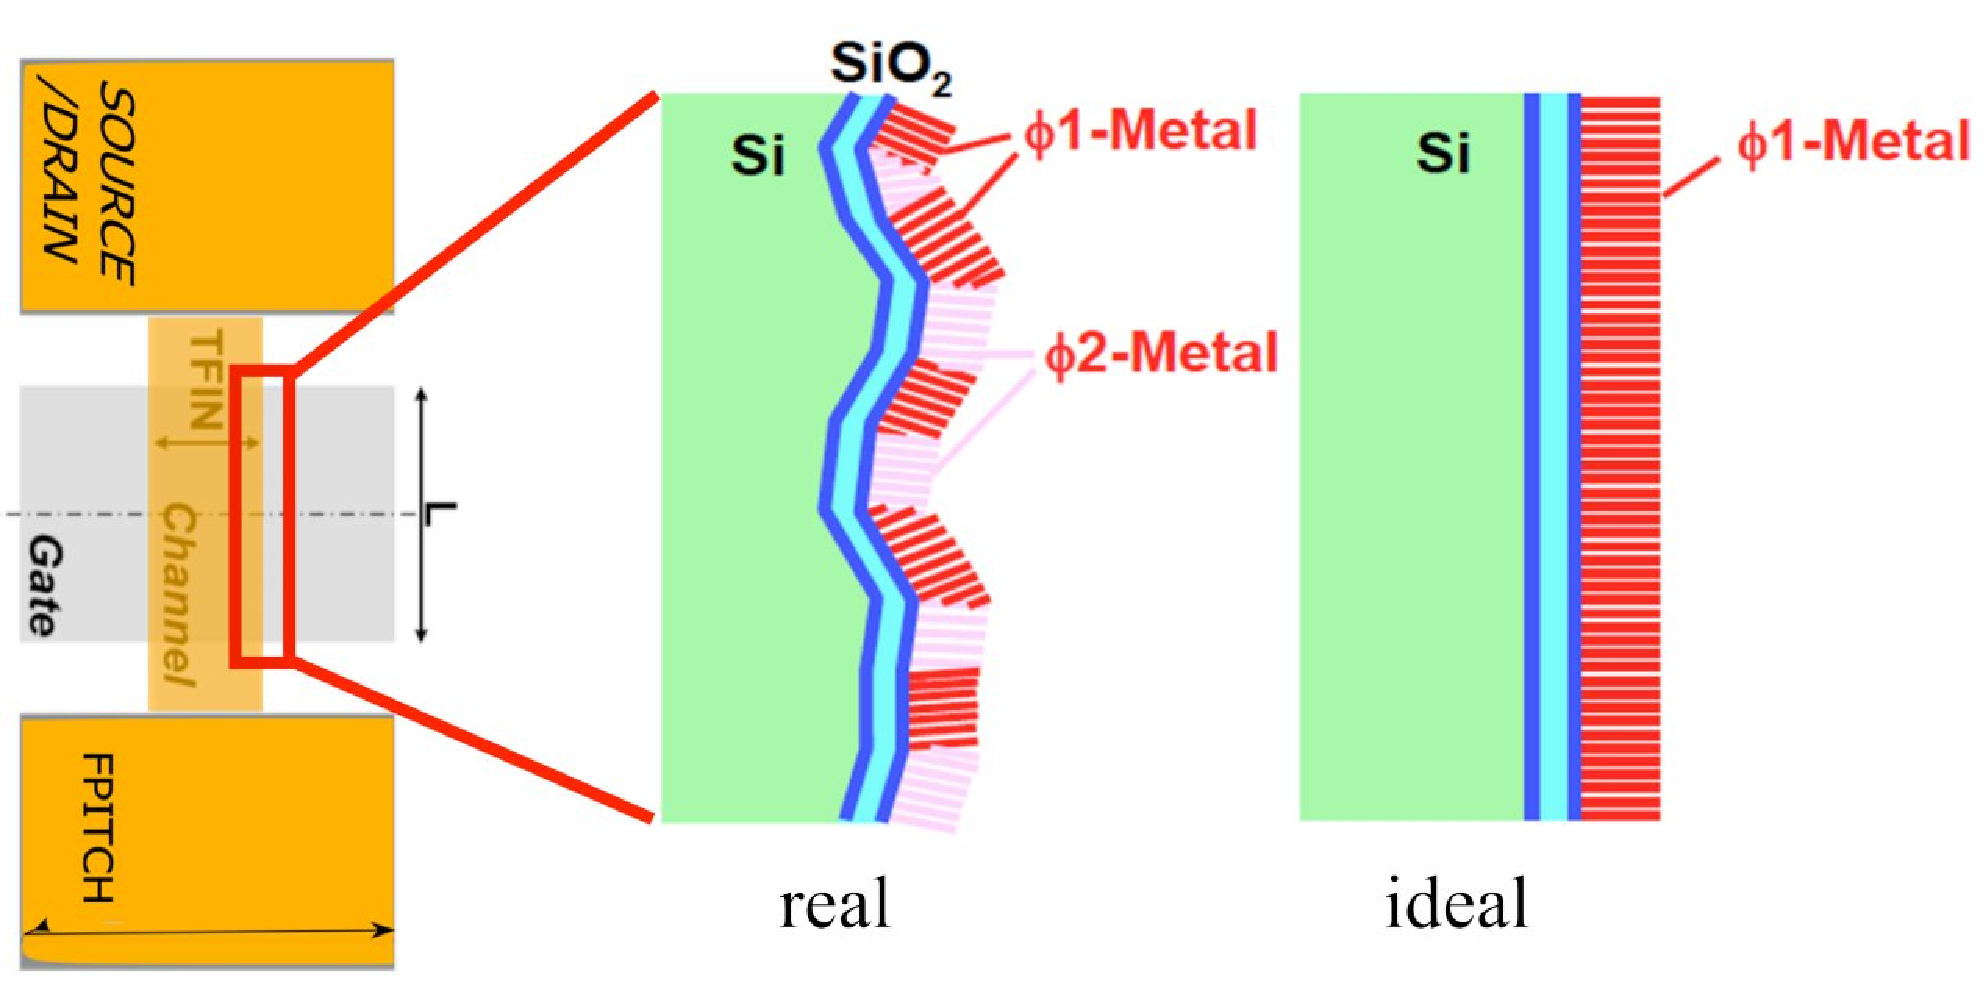
\includegraphics[width=0.75\textwidth, trim={0 0 0 0},clip]{chrome_2019-05-15_16-55-31.pdf}
        \caption{Metal fabrication ideal and real aspects.}
        \label{fig:meinMetalFab}
        \legend{Source: \citet{meinhardt2014impact}}
\end{figure}

\begin{figure} [H]
        \centering
        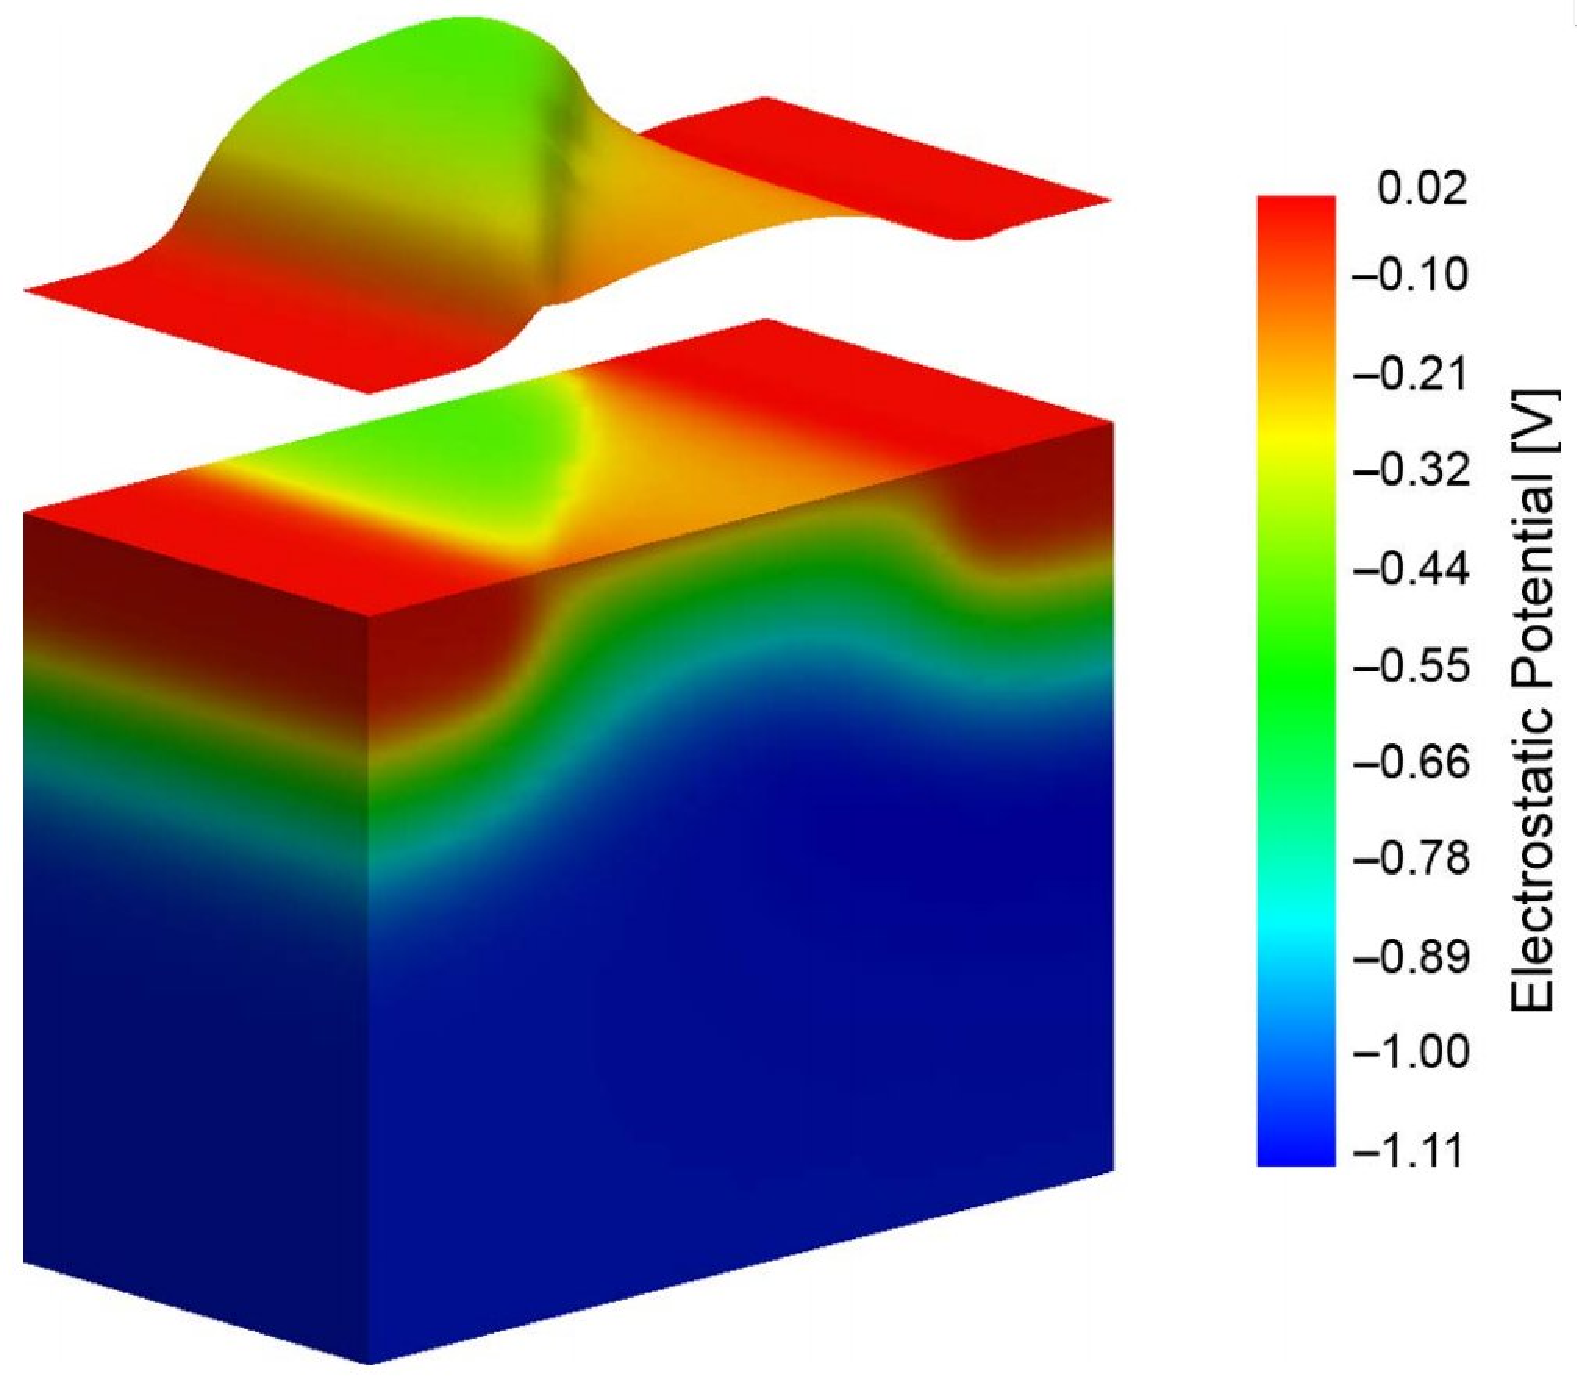
\includegraphics[width=0.65\textwidth, trim={0 0 0 0},clip]{pic-selected-190513-1743-08.pdf}
        \caption{Electrostatic potential in a generic 30-nm MOSFET with the surface potential shown below. The metal gate has two grains with the grain boundary diagonally across the channel.}
        \label{WFFelectros}
        \legend{Source: \citet{brown2010impact}}
\end{figure}

\begin{table}[H]
\centering
\caption{}
\label{tab:WFForient}
\begin{tabular}{ccc}
\hline
\textbf{Orientation}                  & \textbf{Probability} & \textbf{Work Function} \\ \hline
\textbf{\textless{}200\textgreater{}} & 60\%                 & 4.6 eV                 \\ \hline
\textbf{\textless{}111\textgreater{}} & 40\%                 & 4.4 eV                 \\ \hline
\end{tabular}
\legend{Source: \citet{brown2010impact}}
\end{table}

The WFF impact can be better understood when considering the equation \ref{eqn:wffvt}, where the threshold voltage for multigate devices is expressed, where $Q_{SS}$ represents the charge in the gate dielectric, $C_{ox}$ is the gate capacitance, $Q_D$ is the depletion charge in the channel, $f_{ms}$ represents metal-semiconductor work-function difference between the gate electrode and the semiconductor, $f_f$ is the fermi potential. Additionally, the fermi potential for the P-type silicon is given by equation \ref{eqn:ff}, where $N_A$ is the acceptor concentration and $n_i$ is the intrinsic carrier concentration \cite{colinge2008finfets}. The effects of $Q_D$ and $Q_{SS}$ onto the threshold voltage ($V_{th}$) are almost negligible compared to $f_f$, in ultrathin body and lighly doped devices, like the FinFET. Additionally, $V_{in}$ is the additional surface potential to $2f_f$, of ultrathin body devices, that is needed to accumulate enough inversion charges into the channel region of the transistor to reach the threshold point \cite{mustafa2013threshold}.

    \begin{equation}
        \centering
        \label{eqn:wffvt}
        V_{th} = f_{ms} + 2f_{f} + \frac{Q_D}{C_{ox}} - \frac{Q_{SS}}{C_{ox}} + V_{in}
    \end{equation}

    \begin{equation}
        \centering
        \label{eqn:ff}
        f_{f} = \frac{kT}{q} ln\frac{N_A}{n_i}
    \end{equation}


Several works analyze the FinFET reliability. It is shown in \cite{meinhardt2014impact} the major influence that WF Fluctuations (WFF) exercise over $V_{T}$ variations of several standard cells. In addition, in \cite{wang2011statistical} it was shown the high correlation between the $I_{ON}$ and $I_{OFF}$ currents and $V_T$ fluctuations due to the granularity of the metal gate.

In \cite{FinFET01} it is shown, at 14/16nm fabricated bulk FinFET technology, that for high energy charged particles, the drive current is the dominant factor to the transient fault pulse width and cross-section. And low energy particles have a grater dependence on secondary transistor and circuit design factors (number of fins, transistor arrangement, etc).

In \cite{FinFET02} the HCI effect is analyzed in pass-gate FinFET transistors. The tests were executed using commercial FinFET technology showing a 50\% chance of errors due to HCI in pass-gate transistors. In \cite{FinFET03} a analysis of the sensitivity of double-gate and FinFET devices to process variations is shown. It is concluded that for 20nm FinFET devices large channel doping concentration is necessary to obtain suitable values of $V_T$ if heavily doped polysilicon gates are used. Due to the small volume of the channel the channel doping will bring unacceptable $V_T$ fluctuations. Given that, heavily doped polysilicon may not be a viable choice with the work function adjustment being a better approach.

In \cite{FinFET04} the modeling of the reliability degradation of a FinFET-based Static Random Access Memory (SRAM) is shown. It is concluded that the probability of failure due to NBTI and Gate Oxide Break Down (GOBD) is relatively lower in comparison to HCI-induced failures. They also shown the improvement of lifetime due to Error-Correcting Code (ECC) memory. In \cite{FINFET05} a investigation on reliability characteristics of NMOS and PMOS FinFETs is conducted. Based on fabricated FinFETs transistor with 17-27 nm width, it was shown that the life time of FinFET is very dependable of its dimensions. The predicted lifetime for a 50nm gate length NMOS FinFET was 133 years, for the first HCI event. While a 27nm fin-width PMOS FinFET showed 26.84 years of lifetime wich is reduced to 2.76 years when reducing its fin-width from 27 to 17 nm for a NBTI event, showing the huge reliability challenge introduced by technology scaling.



\chapter{Considered Designs}

STs circuits present a hysteresis characteristic. This hysteresis exists in the presence of two switching $V_T$. If the input level is within the hysteresis region, the ST shall not switch. Such characteristic gives a higher static noise margin (SNM) in comparison to traditional inverters, ensuring a high noise immunity.

 Variations in physical parameters became alarming at ultra-deep sub-micron (UDSM) nodes because the node scaling was accompanied by a supply voltage scaling, making the circuits more susceptible to noise and electromagnetic interference due to the deterioration in SNM \cite{pal2018circuit}. Given that, this work explores a two types of STs.

 \section{6T Traditional ST}
 The first is the 6T traditional ST where the main difference from the most common versions is the presence of ${P_F}$ and ${N_F}$ devices as shown in Fig. \ref{fig:ST} \cite{doki1984cmos}. These transistors are responsible for a feedback system. For example, if the output is in a high level, the ${N_F}$ is on, pulling the node ${X}$ to a high potential, and forcing the drain-source voltage of transistor ${N_I}$ almost zero and its gate-source voltage into the negative region. This kind of arrangement reduces the leakage current ${N_I}$ exponentially, increasing the on-to-off current ratio, and minimizing the output degradation \cite{lotze2017ultra}.

The main effect of process variability is a shift on the voltage transfer curve (VTC) due to the threshold voltage variation. Usually, the input voltage, where a device starts delivering current, is directly dependent on the $V_T$. Thus, the variability impact on VTC is reduced in the ST as a result of the high influence of the gate-source voltage of the inner transistor ($N_I$ and $P_I$) over its switching point \cite{lotze2017ultra}.

\begin{figure}[H]
  \centering
    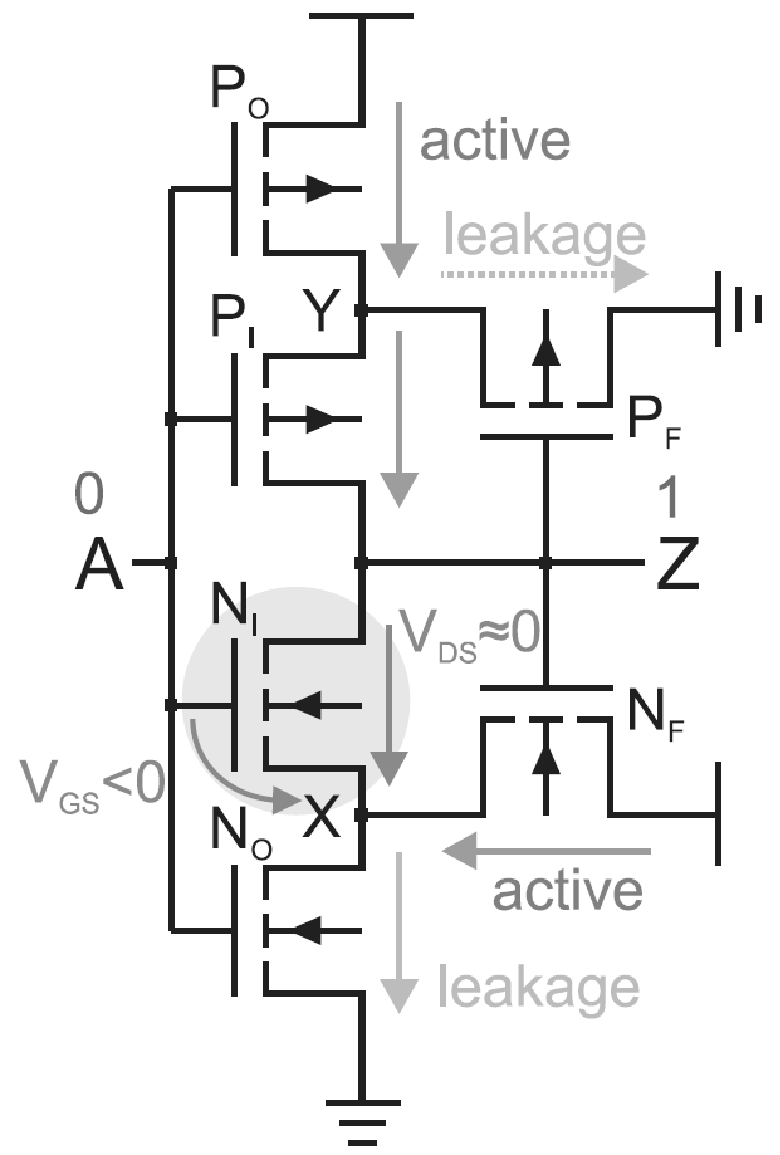
\includegraphics[width=0.4\textwidth]{ST.pdf}
     \caption{ST inverter leakage suppression \cite{lotze2017ultra}.}
  \label{fig:ST}
\end{figure}

\subsection{Three Inverter Schmitt Trigger (TIST)}

The TIST, shown in Fig. \ref{fig:TIST} is a ST implementation, most common in textbooks. It has been mostly unexplored for low power applications. It consists of a CMOS inverter followed by a latch.

\begin{figure}[H]
  \centering
    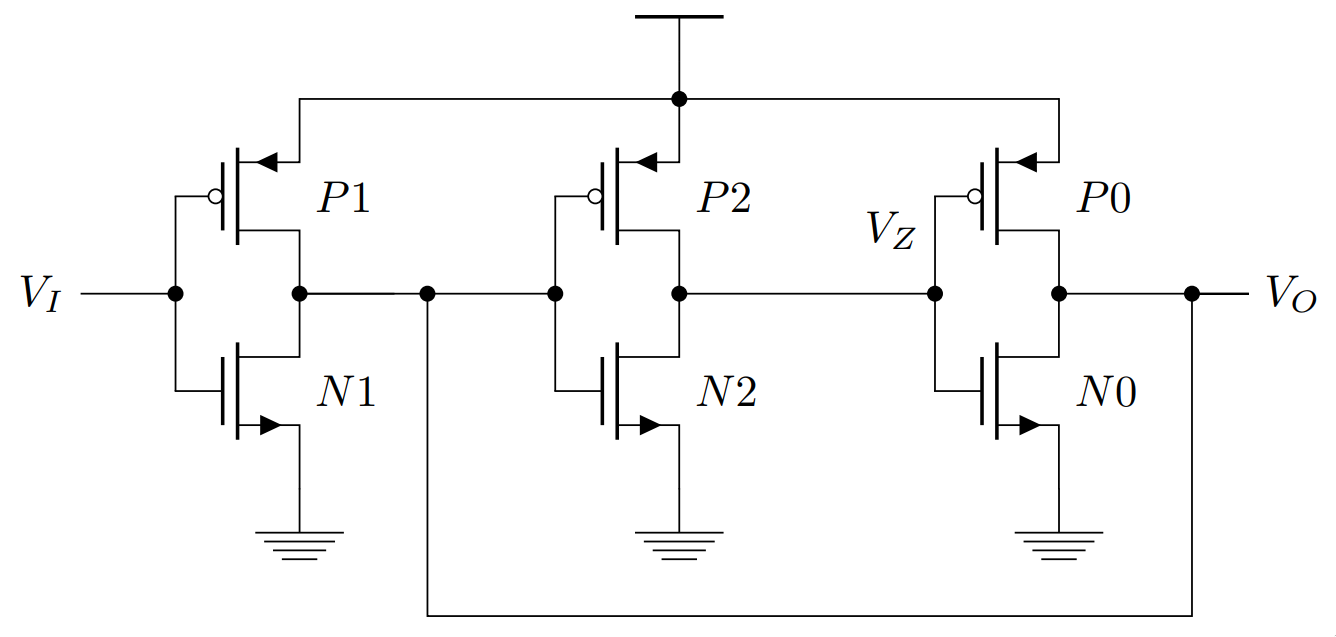
\includegraphics[width=1\textwidth]{TIST.png}
     \caption{TIST schematic \cite{rabaey2002digital}}
  \label{fig:TIST}
\end{figure}

\subsection{Stacked Inverter Gate (SIG)}

SIG, shown in Fig. \ref{fig:SIG}, is a circuit composed of unbalanced inverters without positive feedback, referred to as stacked, or redundant, inverters. It presented improvements over the CMOS inverter regarding voltage gains \cite{bose2018stacked, luo2017sub}.

\begin{figure}[H]
  \centering
    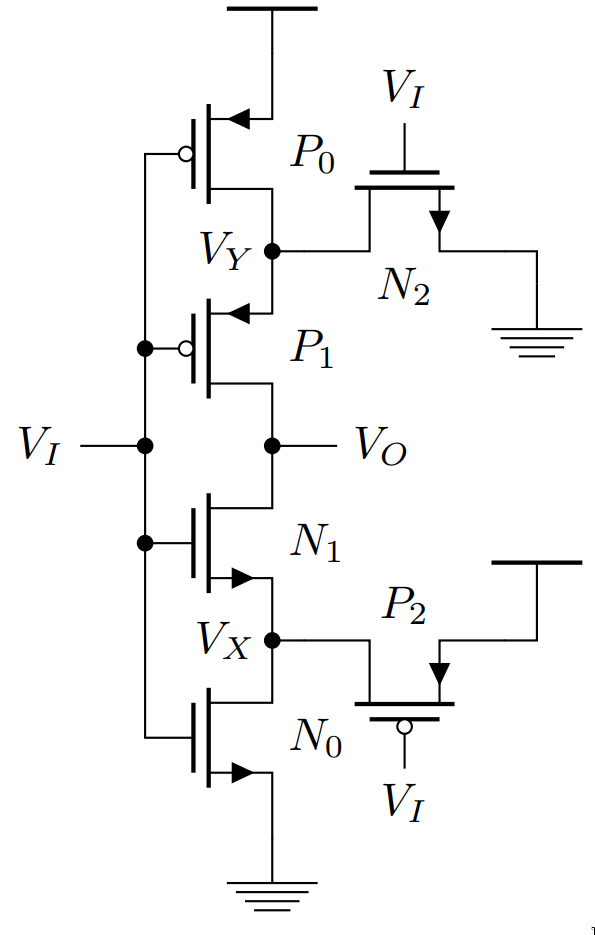
\includegraphics[width=0.4\textwidth]{SIG.png}
     \caption{SIG schematic \cite{bose2018stacked}}
  \label{fig:SIG}
\end{figure}


 A variety of CMOS STs have been proposed and implemented over the years based on different requirements. A higher performance ST is proposed in \cite{steyaert1986novel} where, by a different design, a smaller load capacitor value is achieved, decreasing the slew rate of the ST internal node. In \cite{pfister1992novel} a ST with a programmable hysteresis is proposed. The programmable hysteresis is achieved by adding a P and N transistors in series with the 6T ST $P_F$ and $N_F$ transistors, respectively, both receiving the same gate signal. \cite{kim1993new} proposes a 10T ST which its hysteresis interval does not depend on transistors width/length ratios being, consequently, more robust to process variations.

 A low-power ST is proposed at \cite{al2002low} with low short circuit current achieved by the presence of only one path to each power rail, being recommended for low power, very low frequency applications. In \cite{pedroni2005low} proposes a low-power ST by having only one transistor transmitting (at stable output values), considerably reducing power consumption. STs can be optimised by adequate dimensioning as well as stated in \cite{tache2018reliability} where the OTS technique presented the best metrics for low power applications, in accordance to \cite{zimpeck2016finfet}.

In \cite{shah2020soft} a voltage-booster is applied in the traditional 6T ST in order to replace its pull up network and reduce the number of PMOS transistor to only one. This replacement makes it less vulnerable to the effects of NBTI, which severely affects PMOS devices. It was simulated on 32 nm bulk CMOS technology and was revealed to present an almost negligible delay shift of 0.47\%, with the traditional 6T ST and CMOS inverter presenting 7.2\% and 5.32\% shifts, after three years of simulated NBTI stress, respectively. Furthermore, it presented an improved sensitivity against charged particles of 62.48\% and 55.10\% against the CMOS inverter and 6T ST, respectively. And finally, it presented 168.68\% less deviations in comparison to the CMOS inverter considering process variability. It is important, though, to highlight its 4.315x higher leakage power and potential higher area, given finfet technology restrictions considering the higher number of NMOS transistors (5) in comparison to the traditional 6T ST (3).

In \cite{dokania2015circuit} a novel technique based on the replacement of FA’s internal inverters with low voltage STs for PVT variability robustness improvement is originally introduced and applied on seven different FA designs. The simulations were performed using the 16nm bulk CMOS predictive technology model in SPICE. It presented significant variability improvement up to 4.8x in PDP. Although, the improvements occur at the cost of an increase in the area and power dissipation of each design.

Alongside, in \cite{samuel2016} the ST technique is applied on four FAs. It presented promising results regarding the power deviation due to the process variability with a decrease up to 79\% with a drawback of a significant increase in average energy consumption. The simulations were performed with the 16nm technology predictive technology model in NGSPICE.

This technique is tested in several works: In \cite{ahmad2016single} it is presented a novel Schmitt-trigger-based single-ended 11 Transistor SRAM cell. It analyses its performance against seven different SRAM topologies. The novel cell showed the least energy consumption per operation with the smallest leakage power and a 6.9x higher $I_{ON}$/$I_{OFF}$ ratio. Further PVT variability simulations confirmed the robustness of the design regarding read and write operation. The simulations were carried in 22nm predictive technology using HSPICE. \cite{moghaddam2017design} presents a ST buffer using CNFET. It was evaluated against other two buffers and showed, on average, 68\% higher critical charge and 53\% lower energy consumption and a huge gain considering PVT variability robustness. The simulations were carried in 16nm Stanford CNFET model using HSPICE.

In previous work \cite{moraes2018evaluation} the ST technique is evaluated considering 4 different FAs layouts at 7nm FinFET. 64.74\% and 66.6\% reduction in delay and power deviation was achieved.

STs are commonly used as internal circuits on systems to provide enhanced noise tolerance and robustness against random variations in the input waveforms. On a typical input (non-ST), its binary value will switch at the same point on the rising and falling edges. With a slow rising edge, the input will change near the threshold point. When the switching occurs, it will require current from the supply source. With current being pushed from the supply, it can cause a voltage drop across the circuit causing a shift in the threshold voltage.

If the threshold shifts, it will cross the input causing it to switch again. It can go indefinitely causing oscillation. The same thing can happen if there is noise on the input. STs are applied in these cases to filter noise introducing superior and inferior threshold voltages.



For the experiments, there were considered four different types of Full Adders topologies to evaluate their robustness to process variability with their internal inverters replaced by Schmitt Triggers. The Full Adders listed below have been chosen due to their promising results in related and previous works \cite{ames2016investigating,dokania2015circuit,dokania2013investigation,moraes2018evaluation}:

\begin{enumerate}
    \item Complementary MOSFET Adder (CMOS)
    \item Transmission Gate Adder (TGA)
    \item Transmission Function Adder (TFA)
    \item Hybrid Full Adder
\end{enumerate}

The Mirror Full Adder is considered the most traditional Full Adder topology containing 28 Transistors arranged in a pull-up and pull-down networks, which are logically complementary. It has a full voltage swing and buffered Sum and Cout signal and the advantages of good conductibility and robustness when working with novel technologies and low voltages. However, it has high capacitance because each input is connected to the gate of at least a p-channel metal-oxide-semiconductor (PMOS) and n-channel metal-oxide-semiconductor (NMOS) device additionally, it shows the impact of the pull-up network that makes the circuit slower due to the low mobility of its holes \cite{beckett2002fine} \cite{devadas2017design} \cite{islam2011design}.

Transmission Gate Full Adder \cite{weste1985principles} contains 16 transistors, and is a high speed and low power design. However, shows low driving capability which may be unacceptable in some cases where there is a long chain of full adders due to the increase in delay \cite{islam2011design}. The Transmission Function Adder is based on transmission gates as well, containing 20 transistors, working satisfactorily with low voltages but losing performance when cascaded due to the lack of supply/ground contacts and, consequently, driving capability \cite{navi2009novel}. Both TFA and TGA generate the XOR function (H = A XOR B) followed by an inverter which produces the XNOR function (H’). H and H’ are used to control the transmission gates generating the Sum and Cout outputs. The inverter generates delay between H and H’, which will cause the transmission gates to behave as pass transistors, that may introduce glitches and consequently, increase the power consumption of these cells. Additionally, TGA contains three inverters, one more than TFA. The inverters switching introduce more short-circuit power \cite{shams2000novel}.

Inspired by CMOS and CPL Full Adders architectures, the Hybrid Full Adder \cite{navi2009novel} contains 26 transistors, with the main advantage of a high output signal and low power properties. Although, the design shows high input capacitance for specific input vectors. The Full Adder designs are shown in Figure \ref{fig:FAs}.

\begin{figure}[H]
\centering
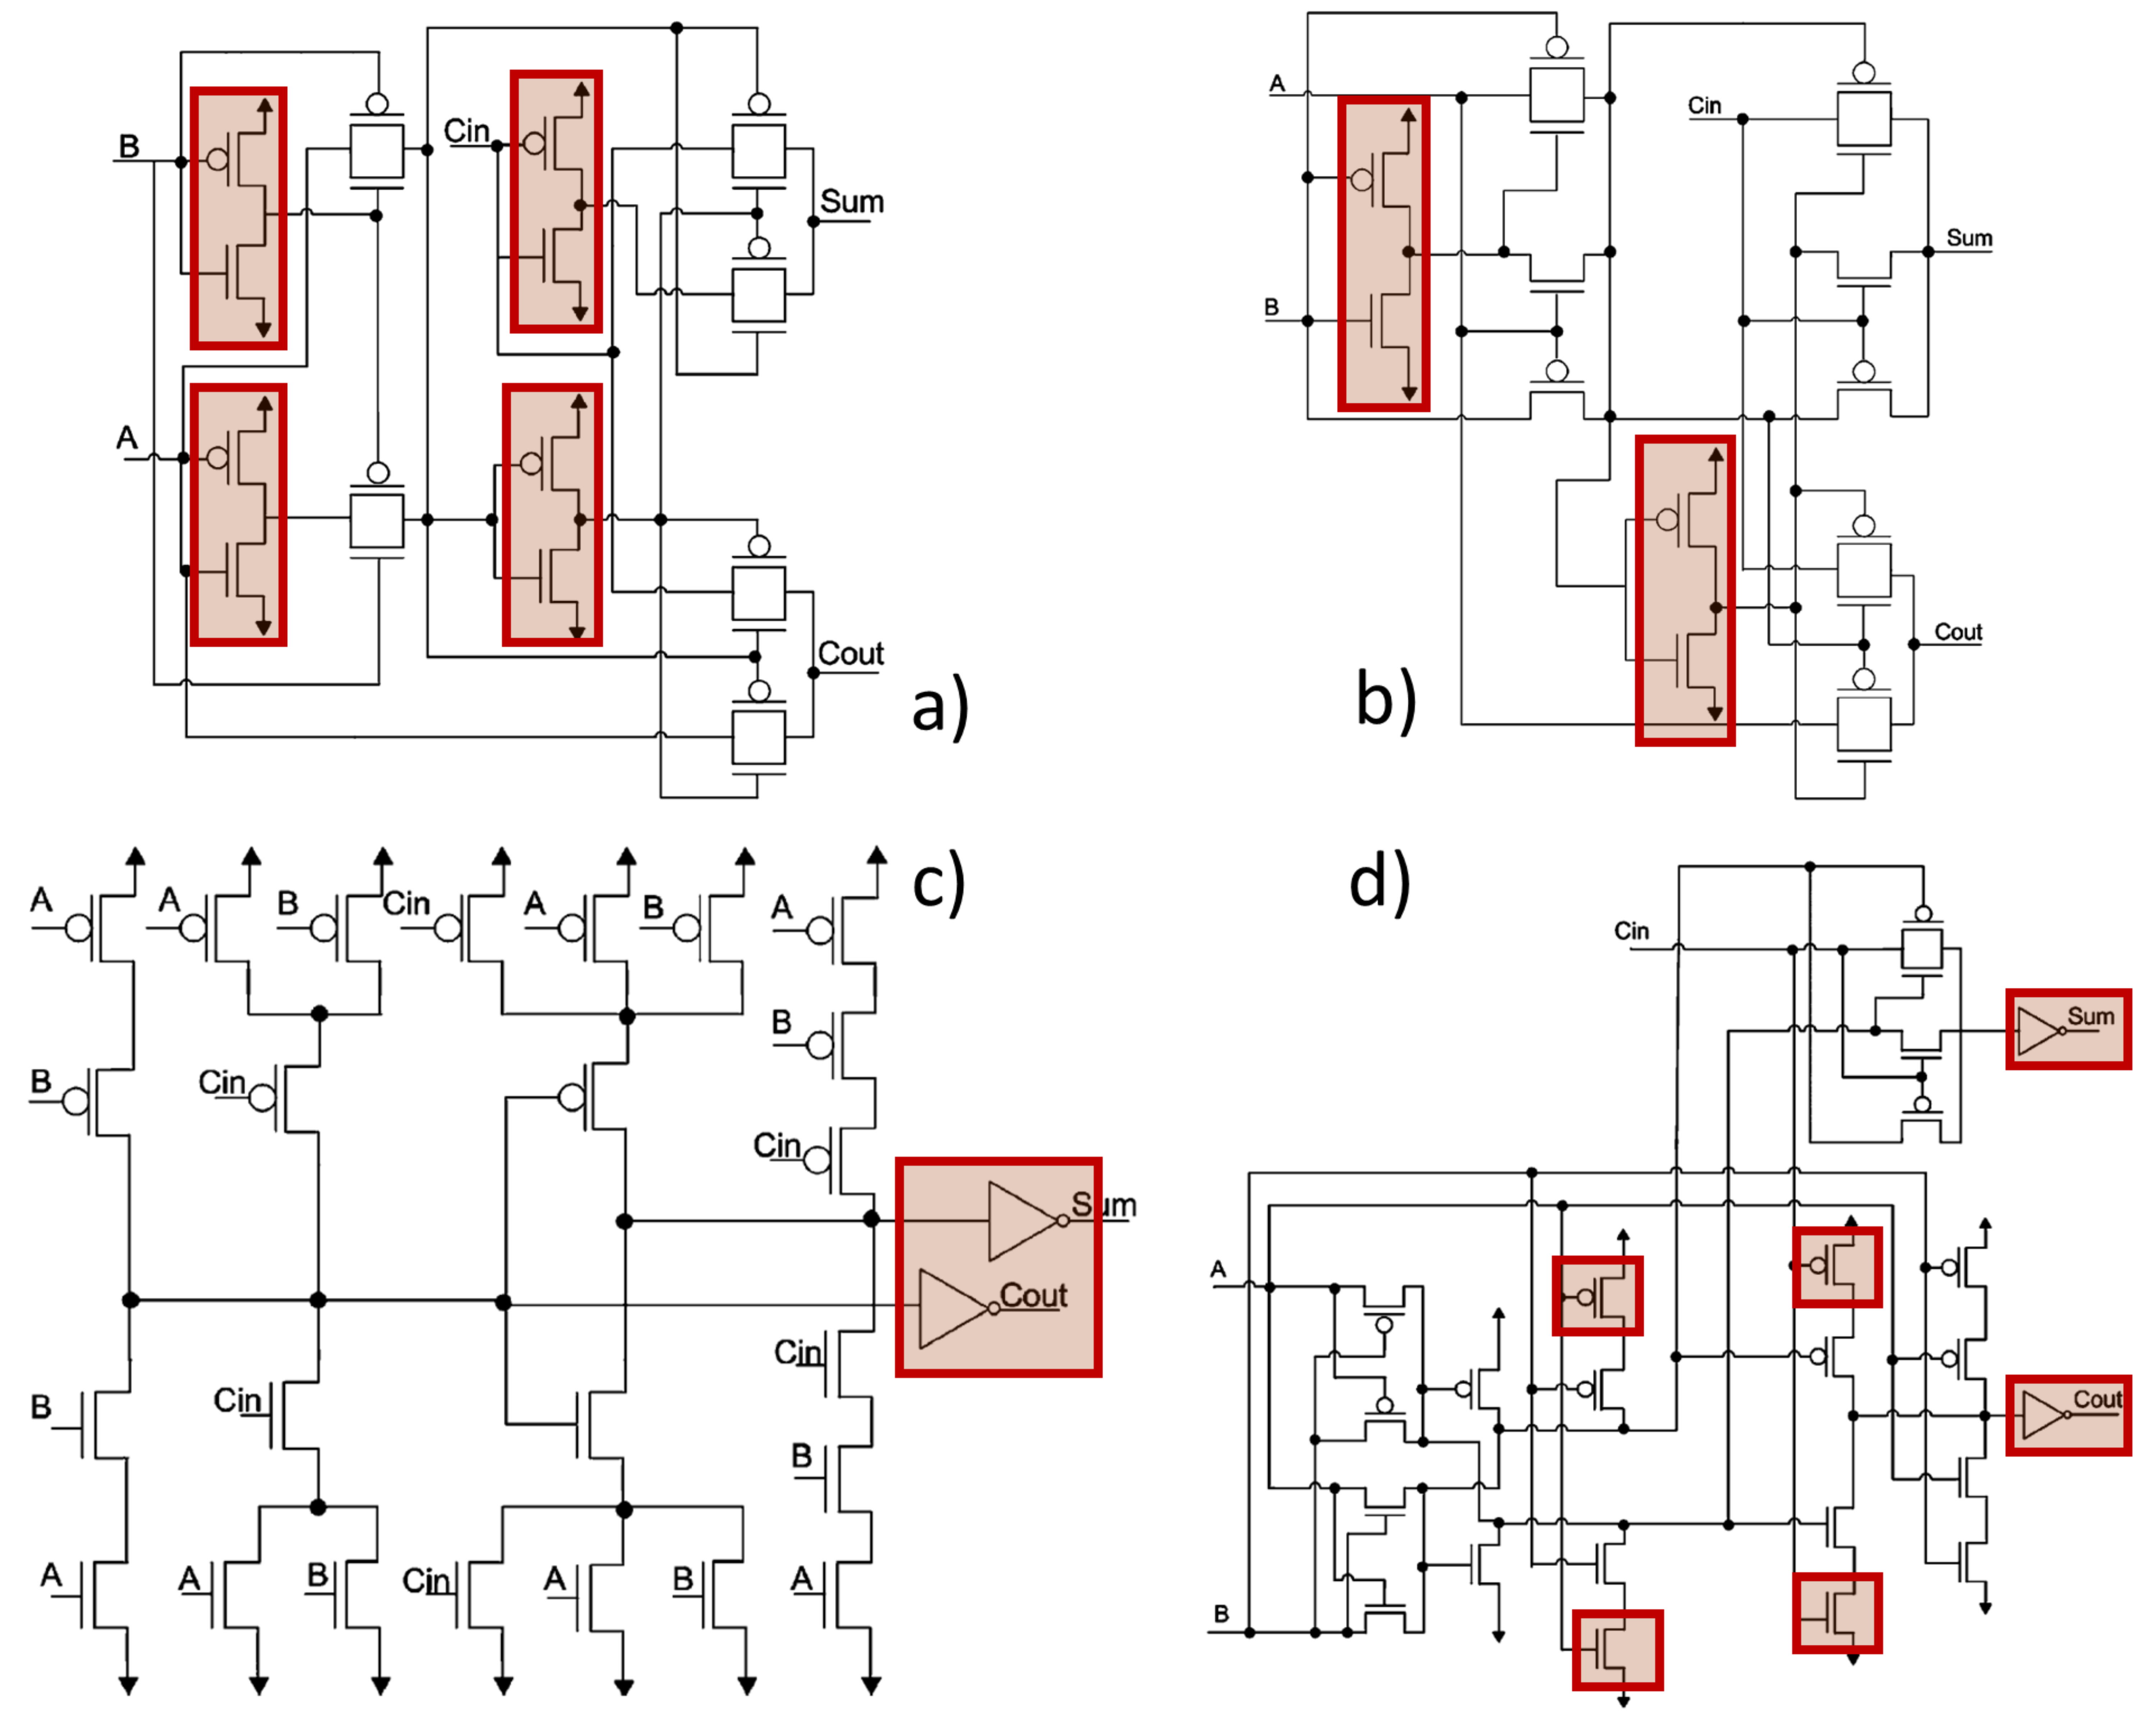
\includegraphics[width=1\textwidth]{FAs.png}
\caption{Full Adders with internal inverters to be replaced highlighted.}
\label{fig:FAs}
\legend{Transmission Gate Adder (a), Transmission Function Adder (b), Mirror CMOS Adder (c) and Hybrid Full Adder (d).
Source: \citet{samuel2016}}
\end{figure}

The additional ST inverter circuit used in this work was inspired by \cite{zhang2003low} and modified in \cite{dokania2015circuit} to achieve the desired inverting characteristic, as shown in Figure \ref{fig:sub1}. It is designed for operation at a supply voltage of 0.4V in order to achieve low power consumption, and consists of the junction of two inverters where the output from the second one will be the bulk for the first one.

In this design a dynamic body-bias technique is applied through a feedback mechanism to a standard CMOS inverter circuit, thus allowing a change in the threshold voltages of two MOSFETs, implying a change in the switching voltage.

\begin{figure}[H]
\centering
\begin{subfigure}{.5\textwidth}
  \centering
  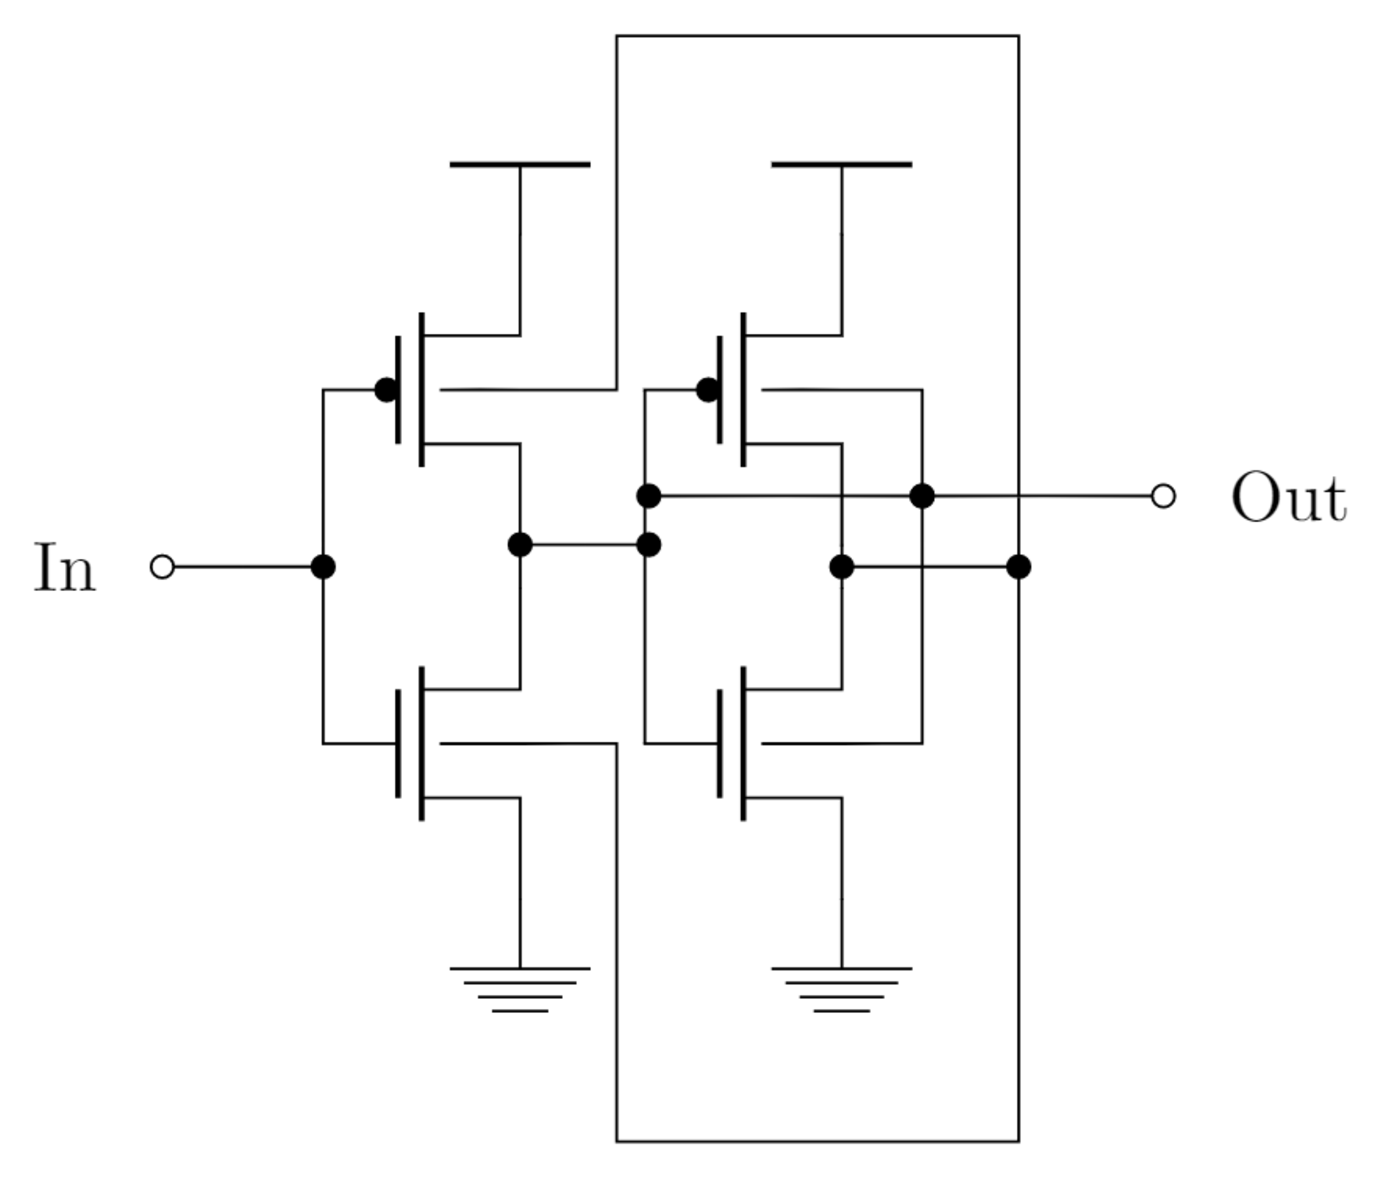
\includegraphics[width=.8\linewidth]{STOriginal.eps}
  \caption{LPST Inverter from \citet{dokania2015circuit}}
  \label{fig:sub1}
\end{subfigure}%
\begin{subfigure}{.5\textwidth}
  \centering
  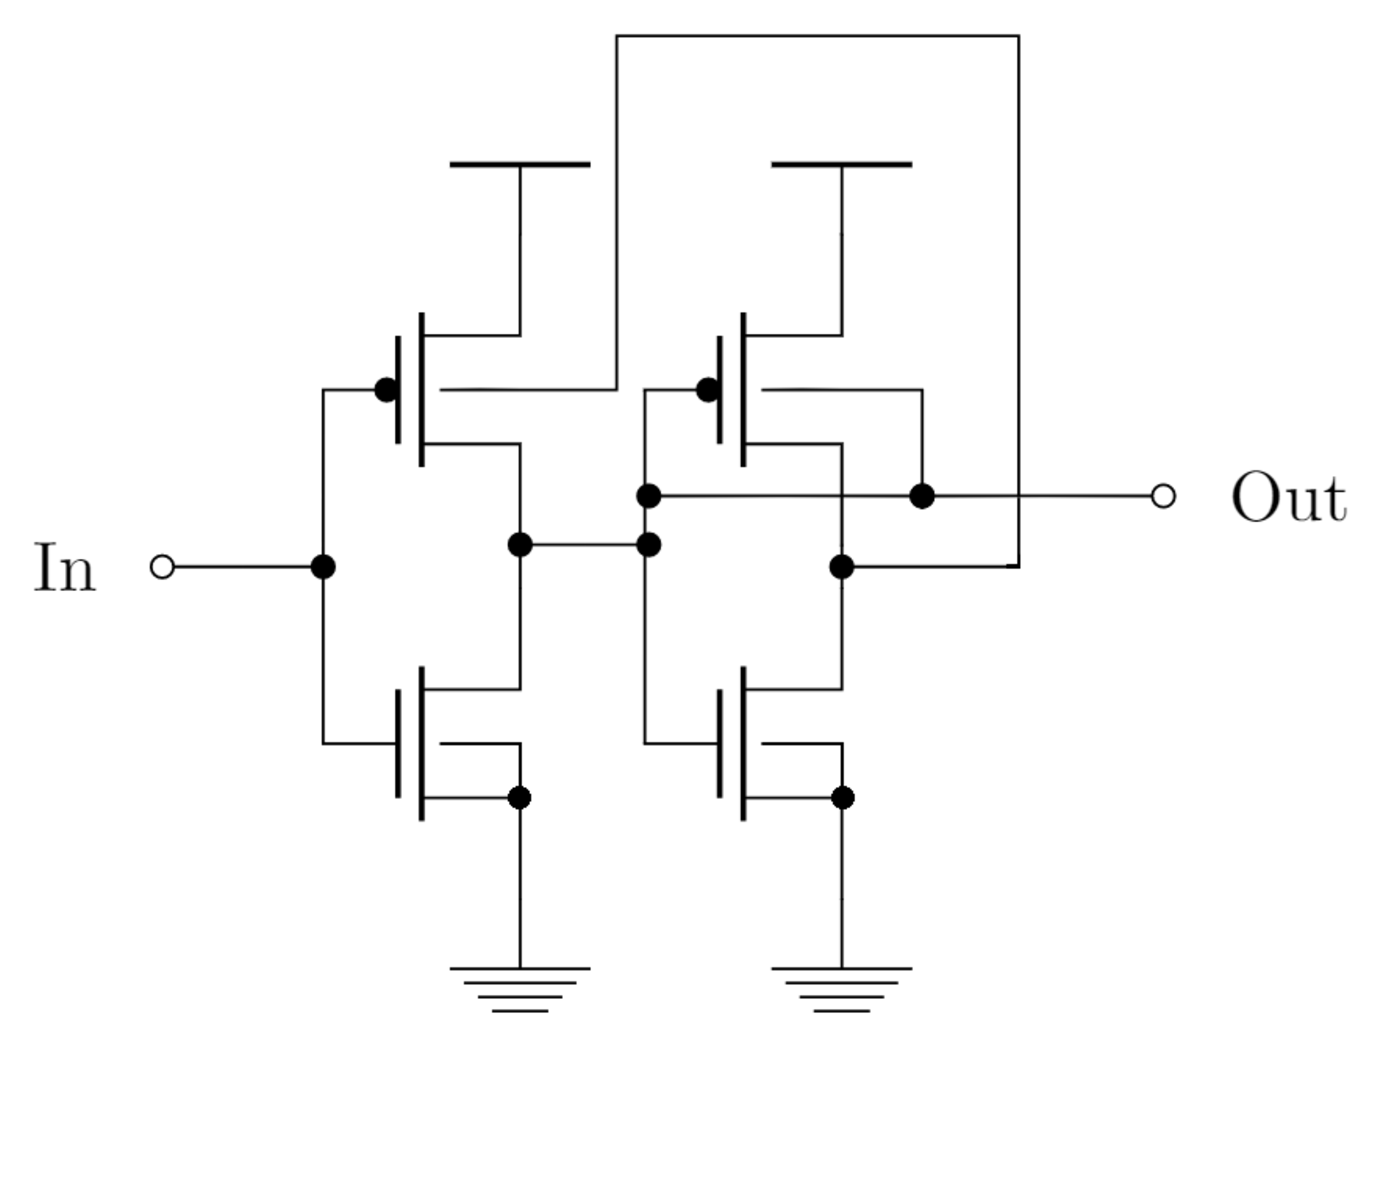
\includegraphics[width=.8\linewidth]{STcorrigido.eps}
  \caption{Modified LPST Inverter applied in this work. Source: From the author.}
  \label{fig:sub2}
\end{subfigure}
\caption{Original and modified Low Power STs (LPST) side-by-side}
\label{fig:test}
\end{figure}

\chapter{Objectives}

Given the laid concepts, this work has two objectives. The first is to identify an appropriate layout, considering the number of fins, and supply voltage in order to achieve a minimum energy device. The considered circuits will be the traditional 6T ST, SIG, TIST and, for the sake of comparison, a traditional inverter. Multiple levels of process variability will be considered. Therefore, depending on manufacturability quality, different recommended layouts and supply voltages can arise. There will be considered the means, standard deviations and normalized standard deviations for each metric, energy, delays on and off currents, current ratios and hysteresis interval (when applicable), respectively.

While, the second objective is to apply the ST technique into FAs, in the case, the CMOS, TFA, TGA and Hybrid FAs. The two ST applied are the traditional 6T ST and the low-power back-gating-based ST from \cite{zhang2003low}. The technique consists of the replacement of the FAs internal inverters with the respective STs. All layouts will be designs with a fixed number of transistors and two levels of supply voltages. All simulations will be performed at the same level of process variability. There will be considered the means, standard deviations and normalized standard deviations for each metric, energy and delays, respectively.

\chapter{Methodology}

To provide an extensive exploration of the process variability effects on the circuits characteristics, this work will evaluate: 1) Circuits operating at multiple combinations of supply voltages; 2) the impact of different levels of process variability; 3) the influence of the transistor sizing; and 4) the impact of these parameters on the maximum achievable frequency within a failure threshold.

The transistor sizing consisted of layouts from 1 to 5 fins through 1-fin steps for the CMOS inverter, the traditional ST and the SIG, since all circuits worked as expected. Since the TIST did not present an adequate behaviour, with its output value getting stuck, a different approach was adopted. The TIST consists of a traditional inverter (transistors $P_1$ and $N_1$) followed by a latch (transistors $P_0$, $P_2$, $N_0$ and $N_2$), given so, the inverter transistors were resized following a proportion between their size and the size of the latch transistors. It was adopted two proportions: 2:1 and 3:1, resulting in five different layouts. Three layouts follow a 2:1 proportion with the inverter transistors containing 2, 4, and 6 fins and the latch transistors containing 1, 2, and 3 fins, respectively. Two layouts follow a 3:1 proportion with the ST transistors containing 3 and 6 fins, and the latch transistors containing 1 and 2 fins, respectively. For the sake of simplicity TIST layouts will be refered to as TIST2F1F, TIST4F2F, TIST6F3F, TIST3F1F and TIST6F2F. With such sizing, the TIST worked properly in most cases, with near-threshold voltage operations presenting the highest number of failures.

According to \cite{thiagoTIST}, the TIST is able to provide hysteresis from a supply voltage as low as the classical inverter unity gain. However, for higher supply voltages, the hysteresis interval will grow excessively to a point where the cell locks itself in a random state (low or high), which cannot be changed. Futhermore, it was shown that the hysteresis interval and the minimum suppyl voltage for it to appear greatly benefit from increase the ratio between the latch and inverter transistors. Given so, in order to tackle some of that problem, the inverter transistors were sized with a higher number of fins in comparison to the latch. Still, it shows the TIST viability to work at sub 100mV supply voltages, which will be explored in future works.
% pág 50 dissertacao do thiago



Due to technology restriction it is not possible to decrease the cell height when considering layout with a fin count below 3. In the case of the ST, for the layouts with a fin count below 3, M2 was applied to connect the source/drain of the ${P_F}$ and ${N_F}$ transistors to the X and Y layout nodes. For the TIST, for the layouts with less than 3 fins, M2 was necessary to connect the output signal to the $P_2$ and $N_2$ transistors gate. Given the smaller area to work with, it was necessary to apply M2 in order to respect the M1 spacing rules, bringing to light one of the challenges related to a smaller layout. The M2 usage in those cases will increase the design parasitics from the necessary extra vias connecting M1 and M2.

For all the Full Adders layouts it was used a dense 7.5 M2 (Metal 2) track cell, baseline resulting in a 270nm cell height. This corresponds to three fins for each transistor.

 %The ST inverter circuits which will be applied in this work was originally proposed in \cite{doki1984cmos} exhibiting the wanted characteristics of different high-to-low and low-to-high transition threshold voltages, giving rise to hysteresis.

 The project was divided into two main steps: the layouts designing and electrical simulations. After finishing the layout design process, each layout passed through validation which consisted of a Design Rule Checking (DRC) to detect if the layout obeys the technology geometry restrictions and layer rules, Layout Versus Schematic (LVS) where layout and schematic are compared to detect their equivalence (same nodes and nets) and a Behavioral test, in order to observe if the circuit works as expected. The design flow is shown at Figure \ref{DesignFlow}.

\begin{figure}[H]
\centering
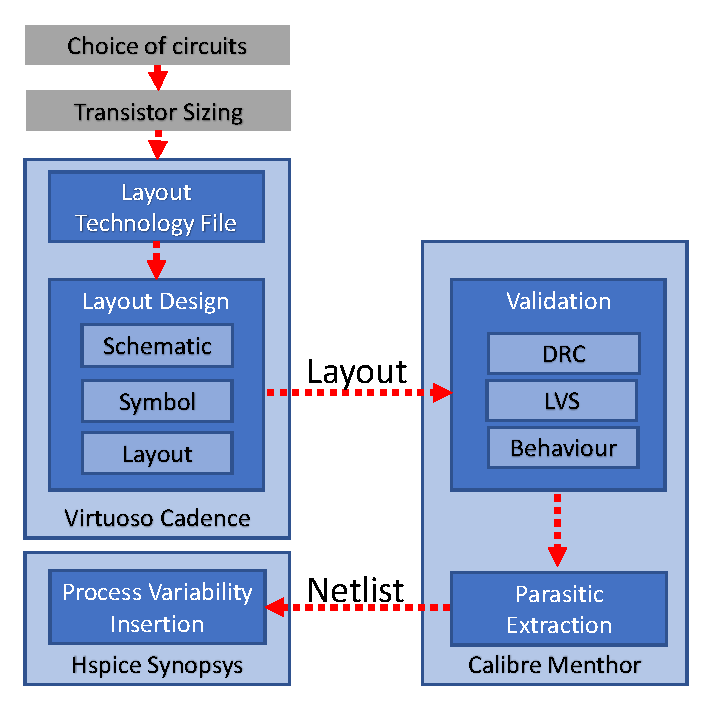
\includegraphics[width=0.8\textwidth, trim={0.25cm 16cm 3cm 0.5cm},clip]{designFlow.pdf}
\caption{Design flow of the experiments.}
\label{DesignFlow}
\legend{Source: From the author.}
\end{figure}

\section{Layout Design}

All circuits were designed using the Virtuoso Electronic Design Automation (EDA) tool from Cadence\textregistered with the process design kit (PDK) of 7-nm FinFET of Arizona State Predictive PDK (ASAP7) from the Arizona State University in partnership with ARM \cite{clark2016asap7}. It is the only available 7-nm PDK for academic use. This PDK was chosen due to realistic design conjecture regarding the current design competencies. FinFET technologies present the width quantization aspect \cite{2000Simulations}. With a 27nm fin pitch, high-density layout is achieved with 3-fins transistors. Otherwise, for a higher fin count, there is a lower density and routing complexity \cite{chava2015standard}. The main PDK rules and lithography assumptions considered in this work are shown in Table I. To exemplify the PDK layers, the 3-fins transistors ST is shown in Fig. \ref{fig:layers}. The dimensions and areas related to each layout is shown at Table \ref{tab:areas}. Figs. \ref{fig:invComp}, \ref{fig:stComp}, \ref{fig:sigComp} and \ref{fig:tistComp} show comparisons between each circuit layouts. In appendix A all layouts can be seen individually. %The ST height with 3, 4 and 5 fins are set to 7.5, 9 and 10.5 tracks of Metal 2 (M2). The total area is 131220nm², 157464nm² and 183708nm² for a design with 3, 4 and 5 fins, respectively. The layout of the ST with 3, 4 and 5 fins are shown in Figs. X, Y and Z, respectively.




\begin{figure}[H]
\centering
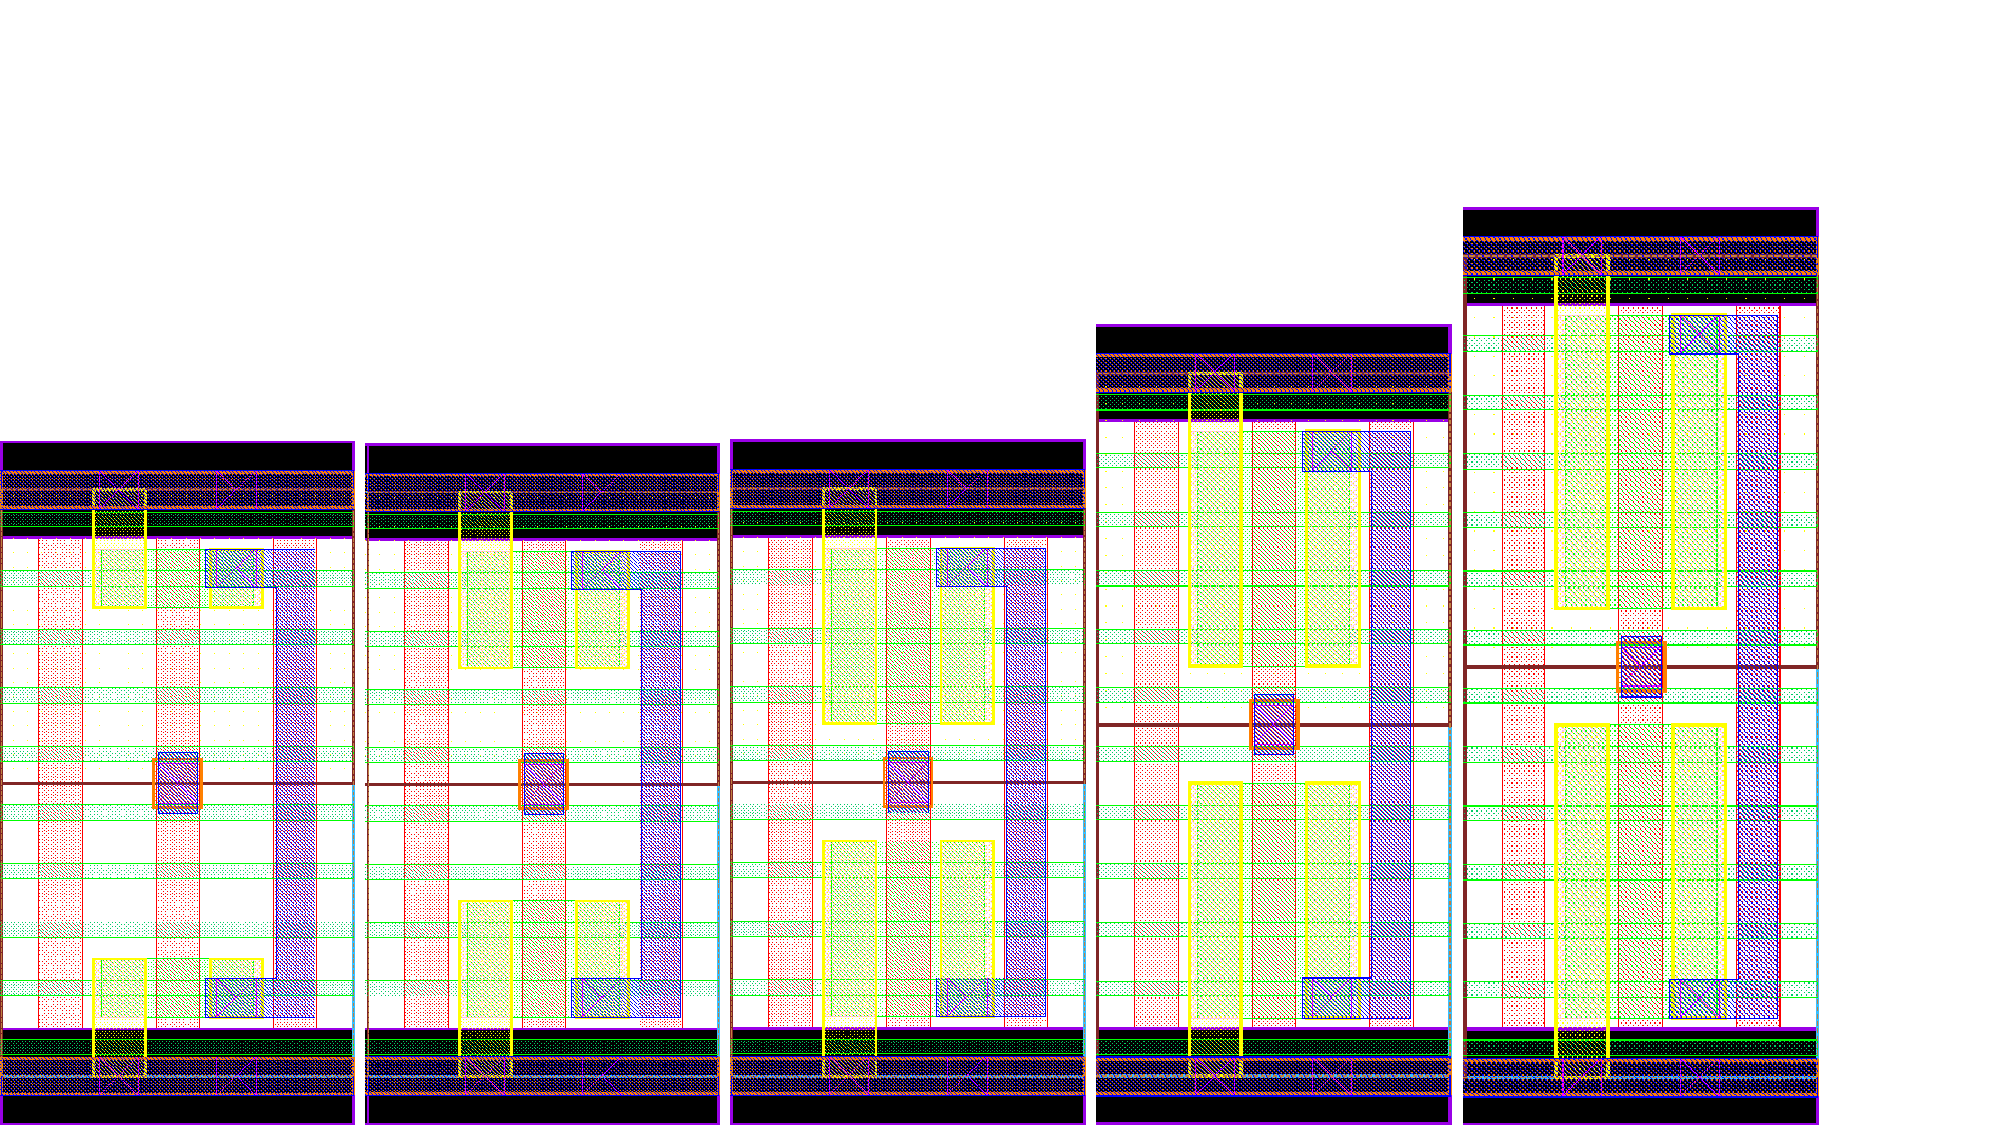
\includegraphics[width=\textwidth, trim={0cm 0cm 4cm 3cm},clip]{INVComp.pdf}
\caption{1 to 5 fins (left to the right) ST layout comparison.}
\label{fig:invComp}
\legend{Source: From the author.}
\end{figure}

\begin{figure}[H]
\centering
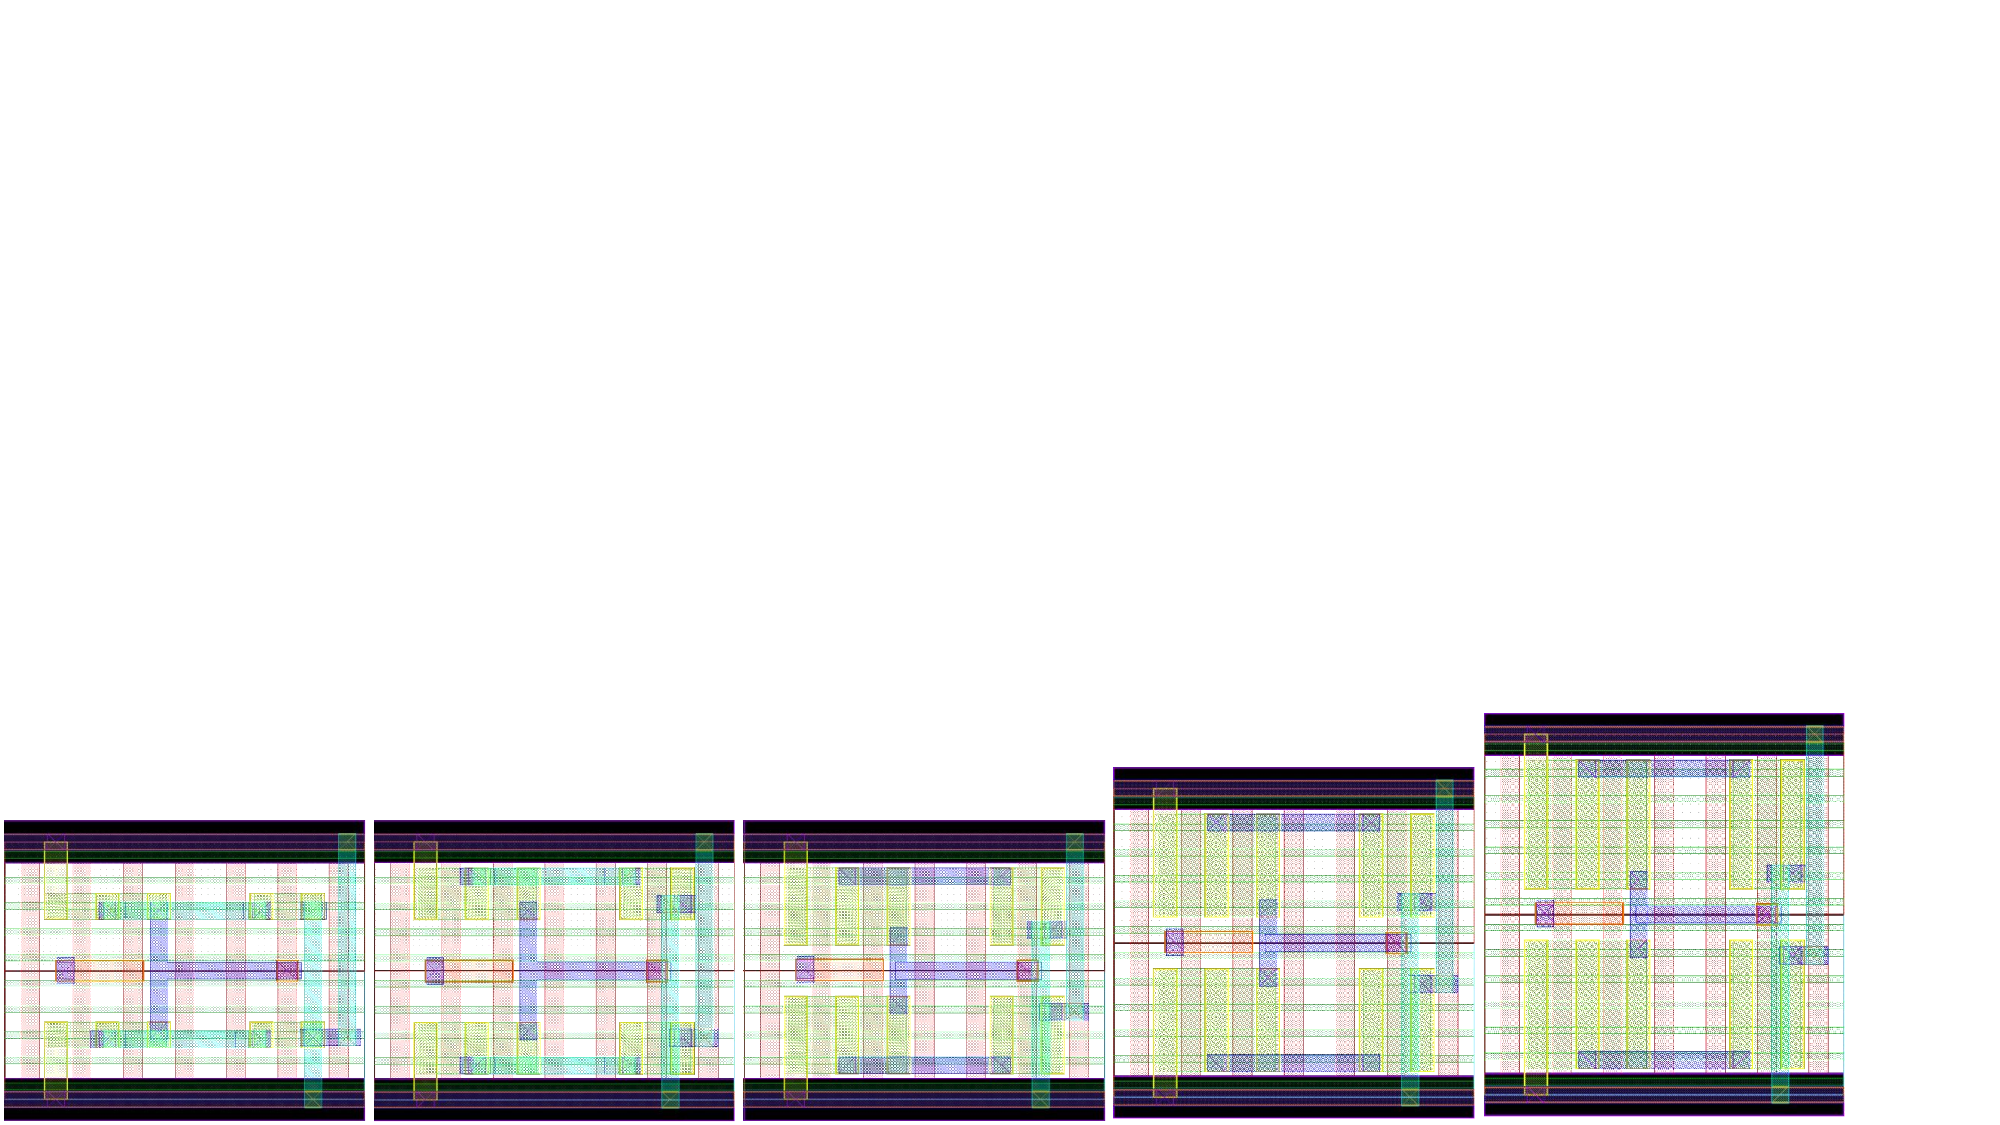
\includegraphics[width=\textwidth, trim={0cm 0cm 3cm 12cm},clip]{STComp.pdf}
\caption{1 to 5 fins (left to the right) ST layout comparison.}
\label{fig:stComp}
\legend{Source: From the author.}
\end{figure}

\begin{figure}[H]
\centering
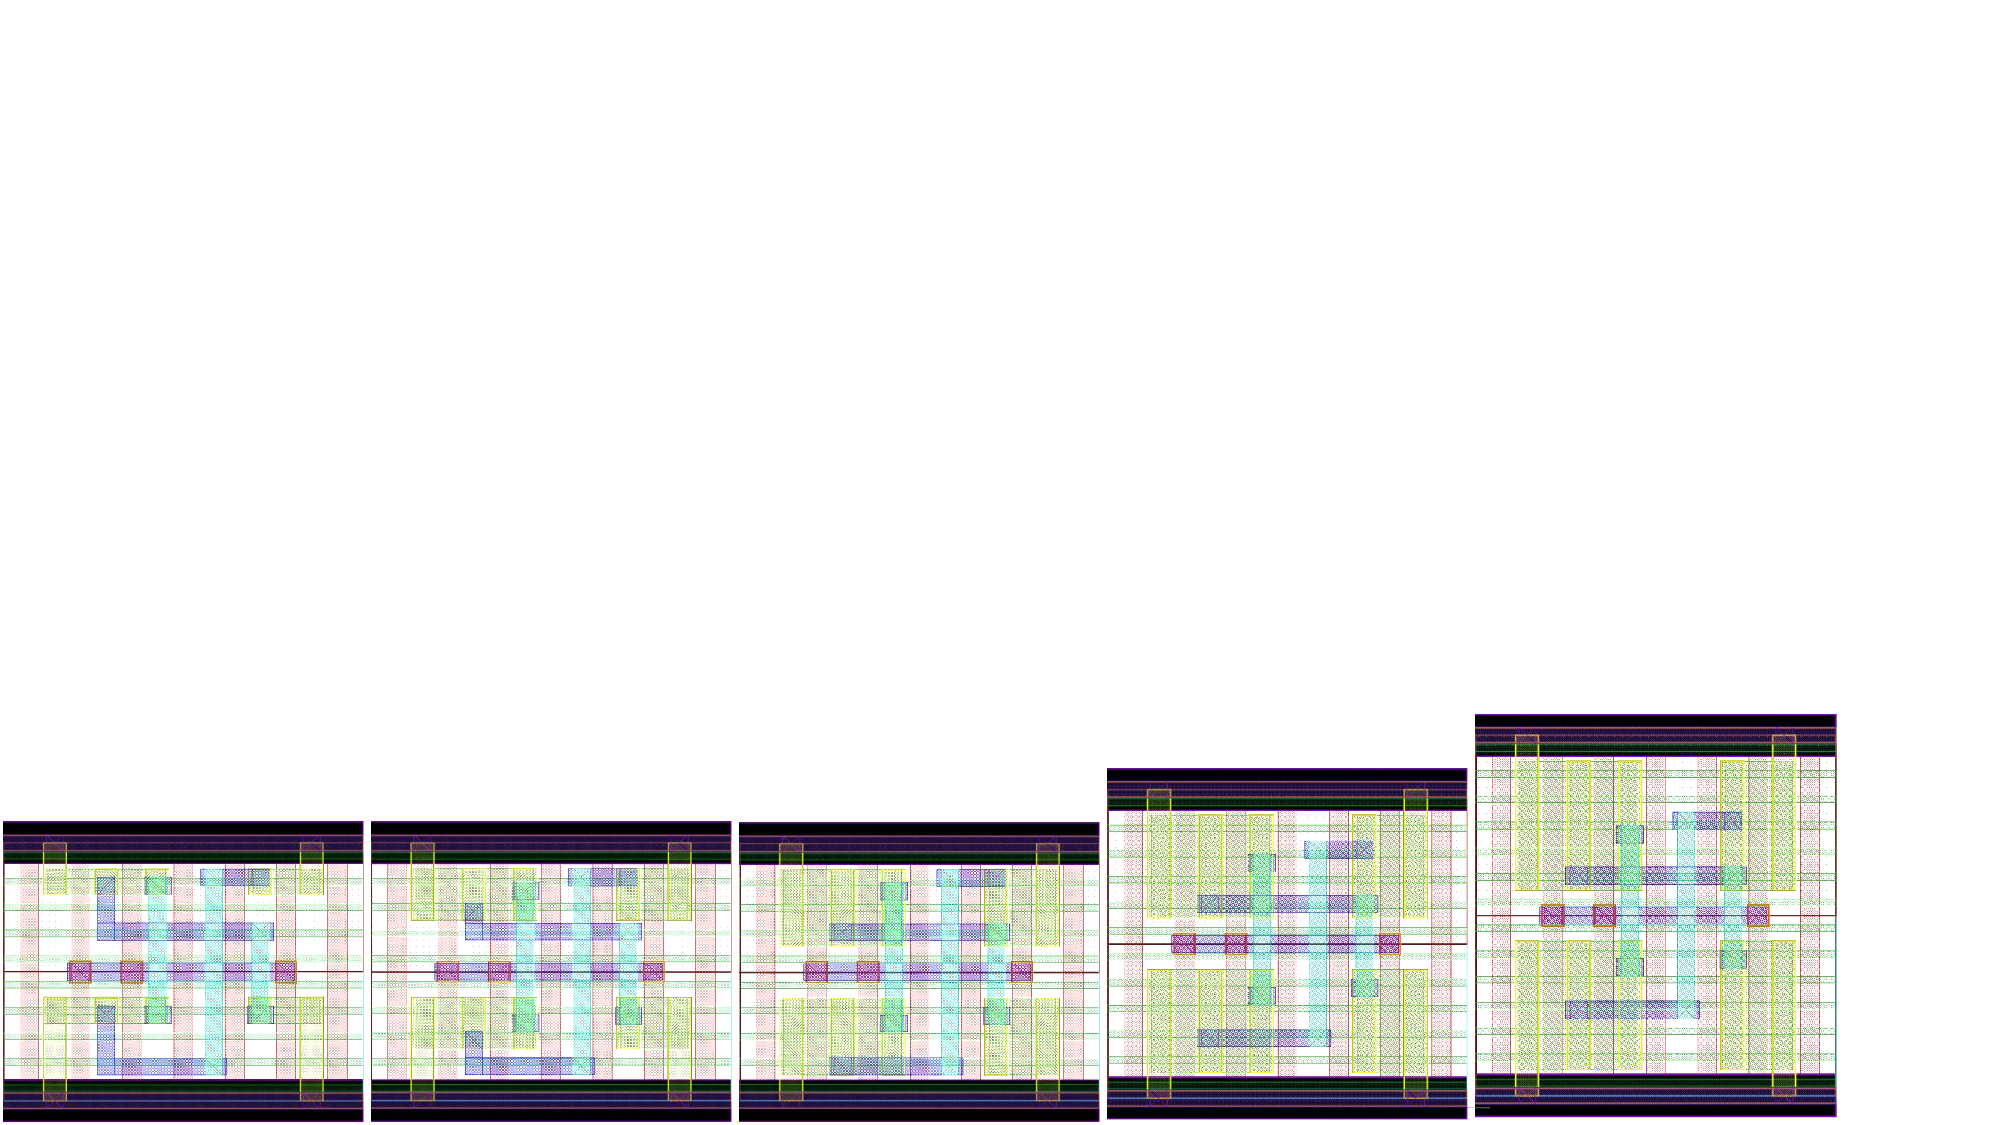
\includegraphics[width=\textwidth, trim={0cm 0cm 3cm 12cm},clip]{SIGComp.pdf}
\caption{1 to 5 fins (left to the right) SIG layout comparison.}
\label{fig:sigComp}
\legend{Source: From the author.}
\end{figure}

\begin{figure}[H]
\centering
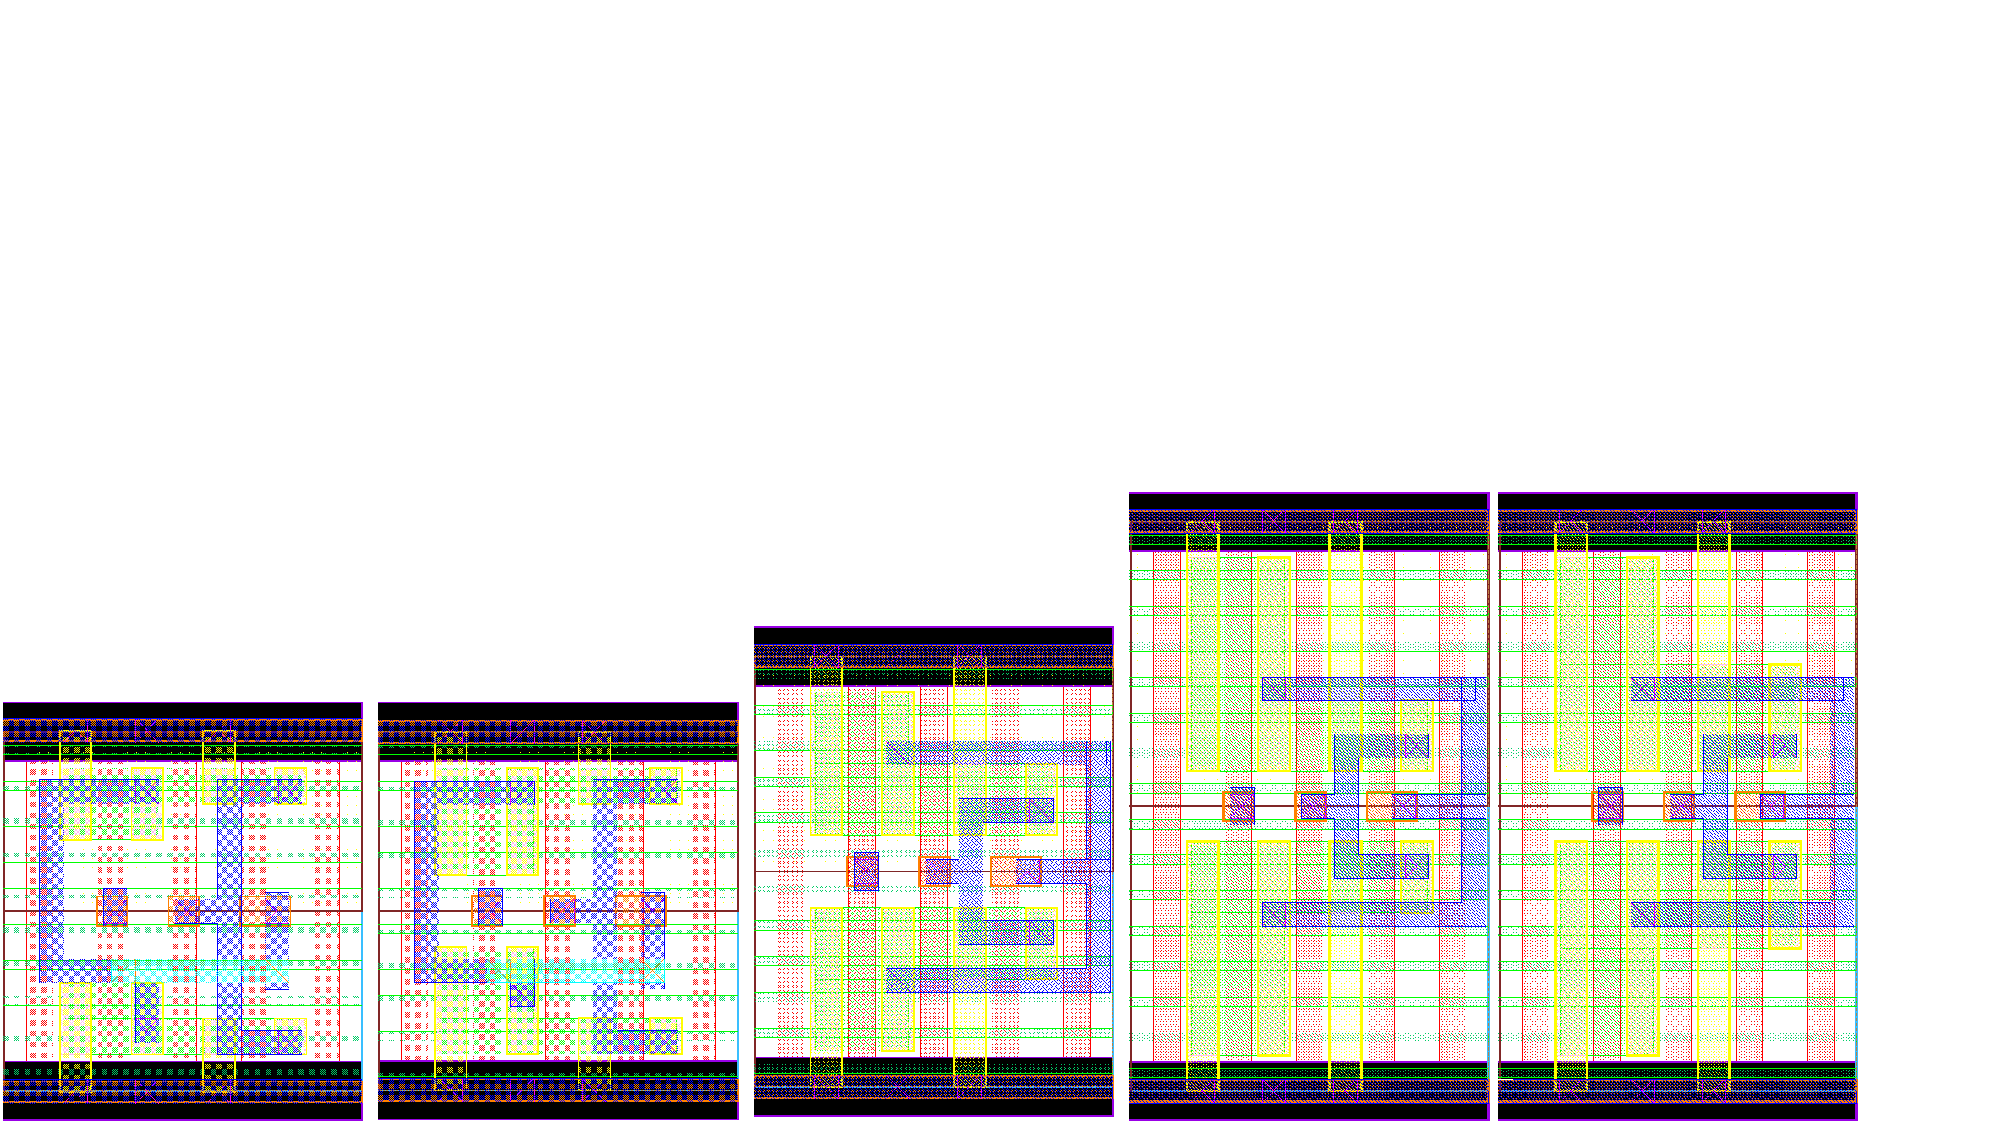
\includegraphics[width=\textwidth, trim={0cm 0cm 3cm 8cm},clip]{TISTComp.pdf}
\caption{From the left to the right, 2, 4 and 6 maximum fins TIST layout comparison.}
\label{fig:tistComp}
\legend{Source: From the author.}
\end{figure}




\begin{table}[H]
\centering
\caption{Key layer lithography assumptions, widths and pitches}
\label{layers}
\begin{tabular}{lccc}
\hline
\multicolumn{1}{c}{\textbf{Layer}} & \textbf{Lithography} & \textbf{Width/drawn (nm)} & \textbf{Pitch (nm)} \\ \hline
\textbf{Fin}                         & SAQP                 & 6.5/7                     & 27                  \\ \hline
\textbf{Active (horizontal)}         & EUV                  & 54/16                     & 108                 \\ \hline
\textbf{Gate}                        & SADP                 & 21/20                     & 54                  \\ \hline
\textbf{SDT/LISD}                    & EUV                  & 25/24                     & 54                  \\ \hline
\textbf{LIG}                         & EUV                  & 16/16                     & 54                  \\ \hline
\textbf{VIA0-VIA3}                   & EUV                  & 18/18                     & 25                  \\ \hline
\textbf{M1-M3}                       & EUV                  & 18/18                     & 36                  \\ \hline
\end{tabular}
\legend{Source: \citet{clark2016asap7}}
\end{table}

\begin{figure}[H]
\centering
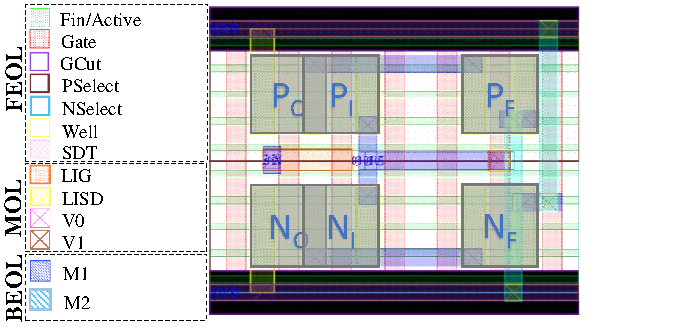
\includegraphics[width=\textwidth, trim={0 0 1.5cm 0},clip]{camadasSTv2.pdf}
\caption{Technology layers and 3-fins transistors 6T ST layout}
\label{fig:layers}
\legend{Source: From the author.}
\end{figure}

%\begin{figure}[H]
%\centering
%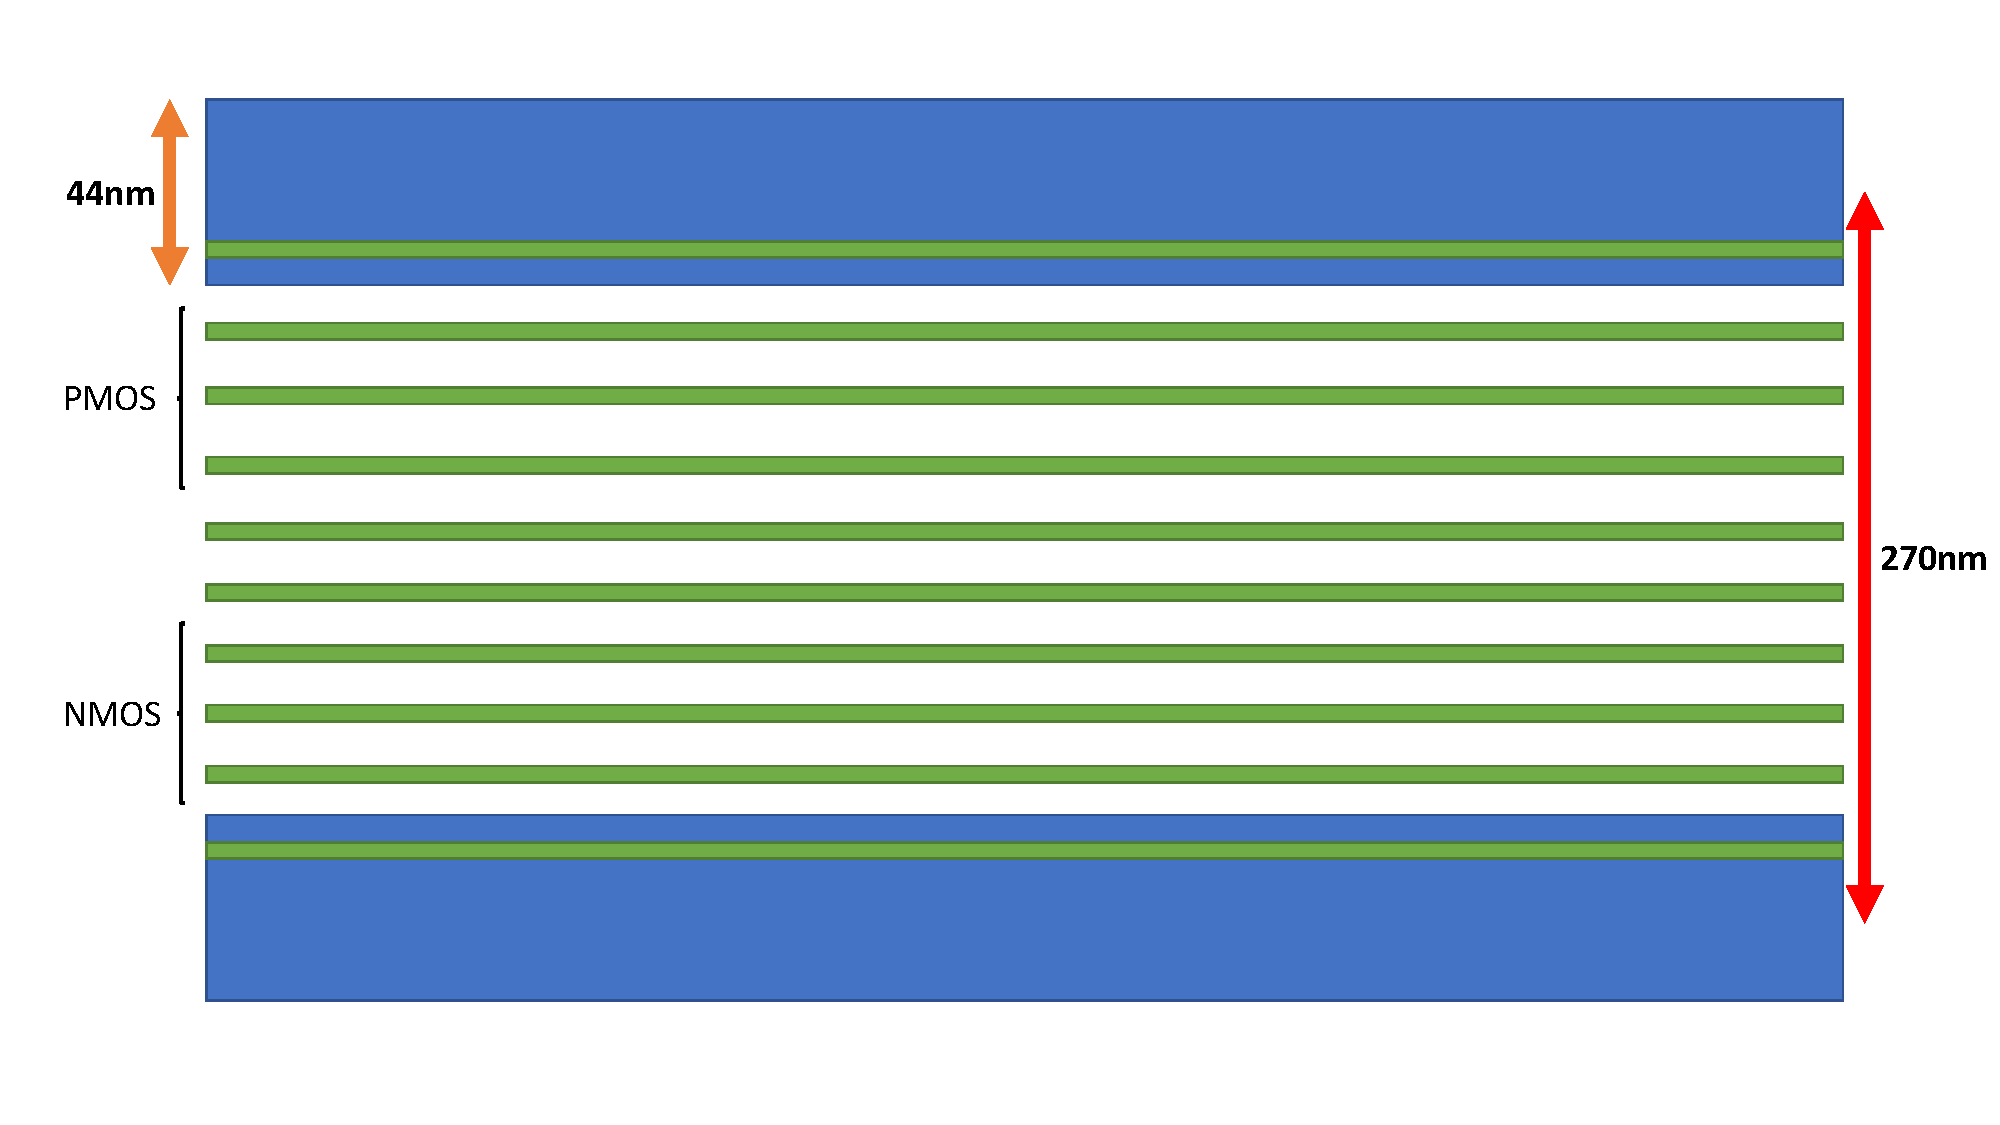
\includegraphics[width=0.8\textwidth]{transistorHeight.pdf}
%\caption{Transistor height and number of fins.}
%\label{th}
%\legend{Source: From the author.}
%\end{figure}



The ASAP7 PDK contains the manufacturing process composed by front end of line (FEOL), middle of line (MOL) and back end of line (BEOL). The layouts were developed in a continuous diffusion layer with every gate surrounding another gate in the horizontal axis. The Source-Drain Trench (SDT) connects the active area to the LISD layer. The Local-Interconnect Gate (LIG) is applied to connect the gate terminal, and Local-Interconnect Source-Drain (LISD) is used to connect the source and drain of the transistors. The function of Via 0 (V0) is to join the LIG and LISD to the BEOL layers. The Metal 1 (M1) is used for intra-cell routing and short connections. The Metal 2 (M2) was applied to connect the PF and NF drains to ground and source, respectively. To make the back-gate connections it is necessary a TAP-Cell. It is responsible to connect the NMOS and PMOS back-gates to supply/ground, respectively, being possible to connect the PMOS back-gates to another node. It is a PDK restriction needed for the proper function of the circuit. Its layout has a length of 108nm resulting in an area of 0.02916${\mu}m^{2}$ the 3-fins variant is shown in Figure \ref{tap}. In order to build the back-gate connections present in the LPST, it was necessary the insertion of TAP-Cells, greatly increasing the layouts size. Each FA area is shown in Table \ref{tab:FAareas} where the LPST and traditional 6T ST are renamed as ST1 and ST2, respectively.

\begin{figure}[H]
\centering
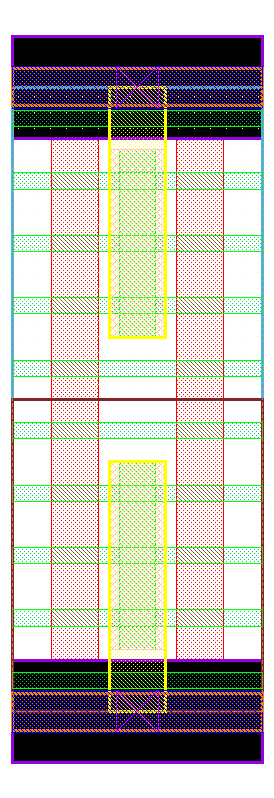
\includegraphics[width=0.2\textwidth]{TAP.png}
\caption{TAP-Cell Layout.}
\label{tap}
\legend{Source: From the author.}
\end{figure}

% Please add the following required packages to your document preamble:
% \usepackage{multirow}
\begin{table}[]
\centering
\caption{Each layout proportion/maximum number of fins, dimension and area (the TAP-Cell area is not taken into account).}
\label{tab:areas}
\begin{tabular}{|c|c|c|c|c|}
\hline
                      & Layout & Height (nm) & Width (nm) & Area (nm²) \\ \hline
\multirow{5}{*}{INV}  & 1 Fin             & 270         & 162        & 43,740  \\ \cline{2-5}
                      & 2 Fins             & 270         & 162        & 43,740  \\ \cline{2-5}
                      & 3 Fins             & 270         & 162        & 43,740  \\ \cline{2-5}
                      & 4 Fins             & 324         & 162        & 52,488 \\ \cline{2-5}
                      & 5 Fins             & 378         & 162        & 61,236 \\ \hline
\multirow{5}{*}{ST}   & 1 Fin             & 270         & 378        & 102,060 \\ \cline{2-5}
                      & 2 Fins             & 270         & 378        & 102,060 \\ \cline{2-5}
                      & 3 Fins             & 270         & 378        & 102,060 \\ \cline{2-5}
                      & 4 Fins             & 324         & 378        & 122,472 \\ \cline{2-5}
                      & 5 Fins             & 378         & 378        & 142,884 \\ \hline
\multirow{5}{*}{SIG}  & 1 Fin             & 270         & 378        & 102,060 \\ \cline{2-5}
                      & 2 Fins             & 270         & 378        & 102,060 \\ \cline{2-5}
                      & 3 Fins             & 270         & 378        & 102,060 \\ \cline{2-5}
                      & 4 Fins             & 324         & 378        & 122,472 \\ \cline{2-5}
                      & 5 Fins             & 378         & 378        & 142,884 \\ \hline
\multirow{5}{*}{TIST} & 2 Fins : 1 Fin             & 270         & 270        & 72,900 \\ \cline{2-5}
                      & 4 Fins : 2 Fins             & 324         & 270        & 87,480  \\ \cline{2-5}
                      & 6 Fins : 3 Fins             & 432         & 270        & 116,640  \\ \cline{2-5}
                      & 3 Fins : 1 Fin             & 270         & 270        & 72,900 \\ \cline{2-5}
                      & 6 Fins : 2 Fins             & 432         & 270        & 116,640  \\ \hline
\end{tabular}
\end{table}

% Please add the following required packages to your document preamble:
% \usepackage{multirow}
% \usepackage{graphicx}
\begin{table}[]
\centering
\caption{Each Full Adder area with the ST technique applied where ST1 and ST2 corresponds to the LPST and 6T ST, respectively.}
\label{tab:FAareas}
\resizebox{\textwidth}{!}{%
\begin{tabular}{|c|c|c|c|c|}
\hline
Full Adder & Width (nm) & Height (nm)           & Area (nm²) & Ratio \\ \hline
CMOS       & 1,188       & \multirow{12}{*}{270} & 320,760     & -     \\ \cline{1-2} \cline{4-5}
CMOS ST1   & 2,808       &                       & 758,160     & 2.36  \\ \cline{1-2} \cline{4-5}
CMOS ST2   & 1,836       &                       & 495,720     & 1.55  \\ \cline{1-2} \cline{4-5}
TGA        & 1,836       &                       & 495,720     & -     \\ \cline{1-2} \cline{4-5}
TGA ST1    & 5,292       &                       & 1,428,840    & 2.88  \\ \cline{1-2} \cline{4-5}
TGA ST2    & 2,916       &                       & 787,320     & 1.59  \\ \cline{1-2} \cline{4-5}
TFA        & 1,620       &                       & 437,400     & -     \\ \cline{1-2} \cline{4-5}
TFA ST1    & 3,240       &                       & 874,800     & 2.00  \\ \cline{1-2} \cline{4-5}
TFA ST2    & 2,052       &                       & 554,040     & 1.27  \\ \cline{1-2} \cline{4-5}
HYBRID     & 1,728       &                       & 466,560     & -     \\ \cline{1-2} \cline{4-5}
HYBRID ST1 & 5,292       &                       & 1,428,840    & 3.06  \\ \cline{1-2} \cline{4-5}
HYBRID ST2 & 2,916       &                       & 787,320     & 1.69  \\ \hline
\end{tabular}%
}
\end{table}

\section{Electrical Simulation}

The simulations will be carried out in HSPICE (https://www.synopsys.com/) using the netlist obtained after the physical verification flow and the parasitic capacitances extraction. The deviation on the device geometry impacts the electrical parameter WF causing high fluctuations \cite{zimpeck2016finfet}. It happens due to the orientation of metal grains randomly aligned in FinFET manufacturing process. In this way, WFF represents the most significant variation beyond the other parameters \cite{meinhardt2014impact}. The process variability evaluation will be taken through 2000 Monte Carlo (MC) simulations \cite{alioto2015variations} varying the WF of devices according to a Gaussian distribution considering a 3\(\sigma\) deviation and variations from 1\% up to 5\% with 1\% steps on nominal values \cite{nawaz2014comparison}. For each step on WF variation, all simulations will be carried from 0.1V to 0.7V supply voltage, with 0.1V steps. The reference values from ASAP7 technology for electrical simulations are shown in Table \ref{electPar}.

\begin{table}[H]
\centering
\caption{Parameters applied in the electrical simulations}
\label{electPar}
\begin{tabular}{lcc}
\hline
\textbf{Parameter}                                            & \multicolumn{2}{c}{\textbf{7nm}}                                  \\ \hline
\textbf{Nominal Supply Voltage}                               & \multicolumn{2}{c}{0.7 V}                                         \\ \hline
\textbf{Gate Length (L\textsc{g})}           & \multicolumn{2}{c}{21nm}                                          \\ \hline
\textbf{Fin Width (W\textsc{fin})}              & \multicolumn{2}{c}{6.5nm}                                         \\ \hline
\textbf{Fin Height (H\textsc{fin})}          & \multicolumn{2}{c}{32nm}                                          \\ \hline
\textbf{Oxide Thickness (T\textsc{ox})}      & \multicolumn{2}{c}{2.1nm}                                         \\ \hline
\textbf{Channel Doping}                                       & \multicolumn{2}{c}{$1x10^{22}m^{-3}$}                                     \\ \hline
\textbf{Source/Drain Doping}                                  & \multicolumn{2}{c}{$2x10^{22}m^{-3}$} \\ \hline
\multicolumn{1}{c}{\multirow{2}{*}{\textbf{Work Function (eV)}}} & NFET                            & 4.372                            \\ \cline{2-3}
\multicolumn{1}{c}{}                                        & PFET                            & 4.8108                           \\ \hline
\end{tabular}
\legend{Source: \citet{clark2016asap7}}
\end{table}

For all experiments, it will be observed maximum values, mean (\(\mu\)), standard deviation (\(\sigma\)) and normalized standard deviation (\(\sigma\)/\(\mu\)) for each metric: hysteresis interval, propagation times, energy, and on and off currents where \(\sigma\)/\(\mu\) represents the sensibility of the cell to process variability. The energy was calculated by integrating the current through time and multiplying by the supply voltage, and the propagation times where calculated by the timing difference between input and output signals to reach 50\% of its value ($V_{DD}/2$). Additionally, noise margins, gains and VTC curve slopes will be presented. The noise margins were calculated as shown in Fig. \ref{fig:SNM} where the margin values are extracted from the VTC curve points where the derivative/slope is -1. The slopes were calculated following the equation \ref{eqn:slope}, based on Fig. \ref{fig:SNM}.


\begin{figure}[]
\centering
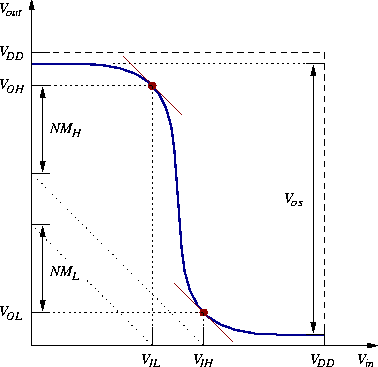
\includegraphics[width=0.8\textwidth, trim={0cm 0cm 0cm 0cm},clip]{img17.png}
\caption{Noise margins measurements.}
\label{fig:SNM}
\legend{Source: \citet{schrom1997vlsi}.}
\end{figure}

\begin{equation}
    \centering
    \label{eqn:slope}
    Slope = \frac{V_{OH} - V{OL}}{V_{IH} - V_{IL}}
\end{equation}

 For a more realistic test bench, it will be considered a scenario where the Device Under Test (DUT) receives the signal passing through two inverters in series and having a 1fF output capacitance, as shown in Fig. \ref{fig:tbST}. It is essential to consider some details such as: the same supply voltage is applied in the entire testbench, only the DUT suffers from variability, the inverters are the same (3-fins transistors) for all experiments, and they are, like the DUT, simulated from the extracted layout.



\begin{figure}[H]
\centering
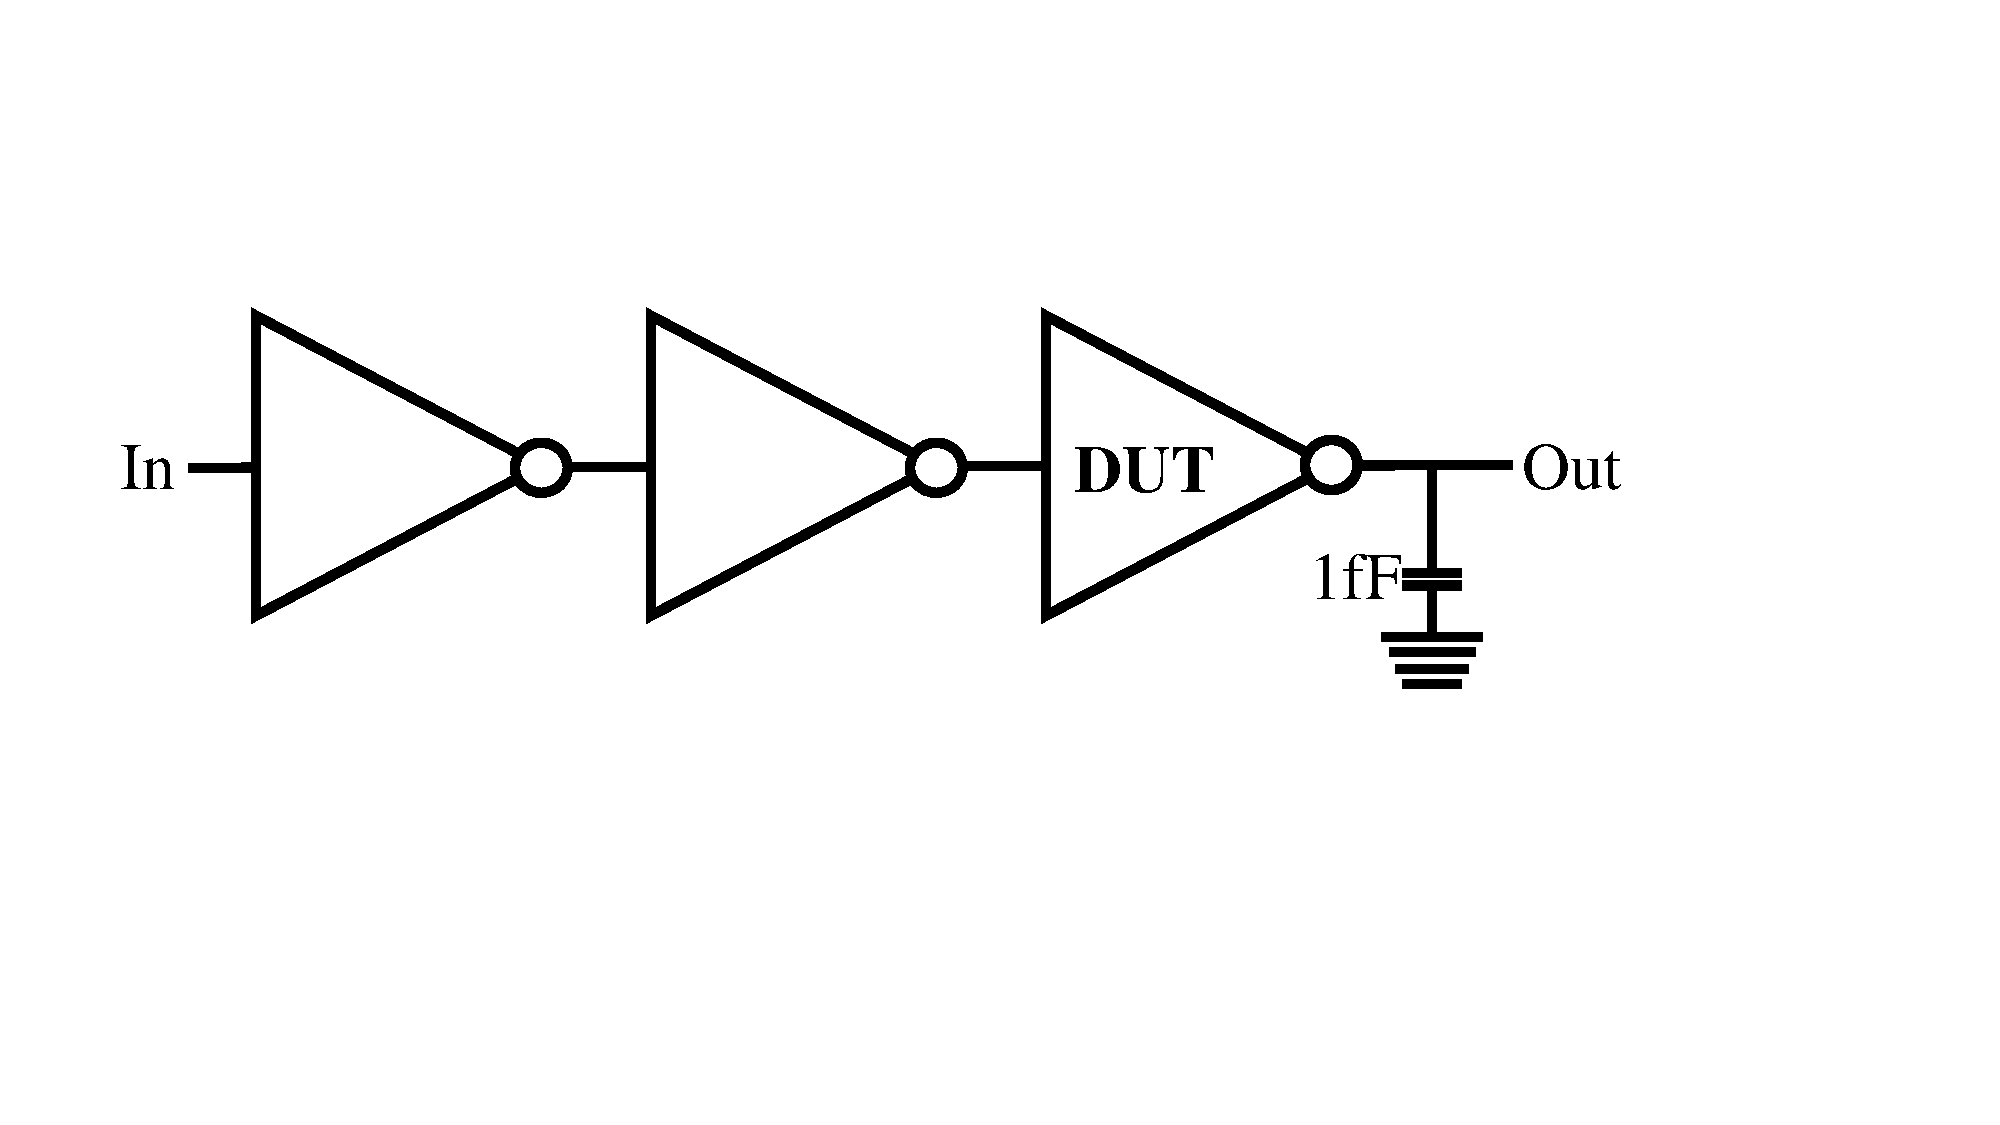
\includegraphics[width=0.8\textwidth, trim={2cm 7cm 6cm 5cm},clip]{testbench.pdf}
\caption{Test Bench.}
\label{fig:tbST}
\legend{Source: From the author.}
\end{figure}

For the simulations concerning the Full Adders, it was considered the mean, standard deviations, and normalized standard deviations for the energy and delay measures. The test bench applied consisted of a 5-bit Ripple Carrier Adder with with each output (Sum outputs for each FA and last Carry Out) connected to a fan-out of 4 inverters, as shown in Fig \ref{fig:tbFA}.

\begin{figure}[H]
\centering
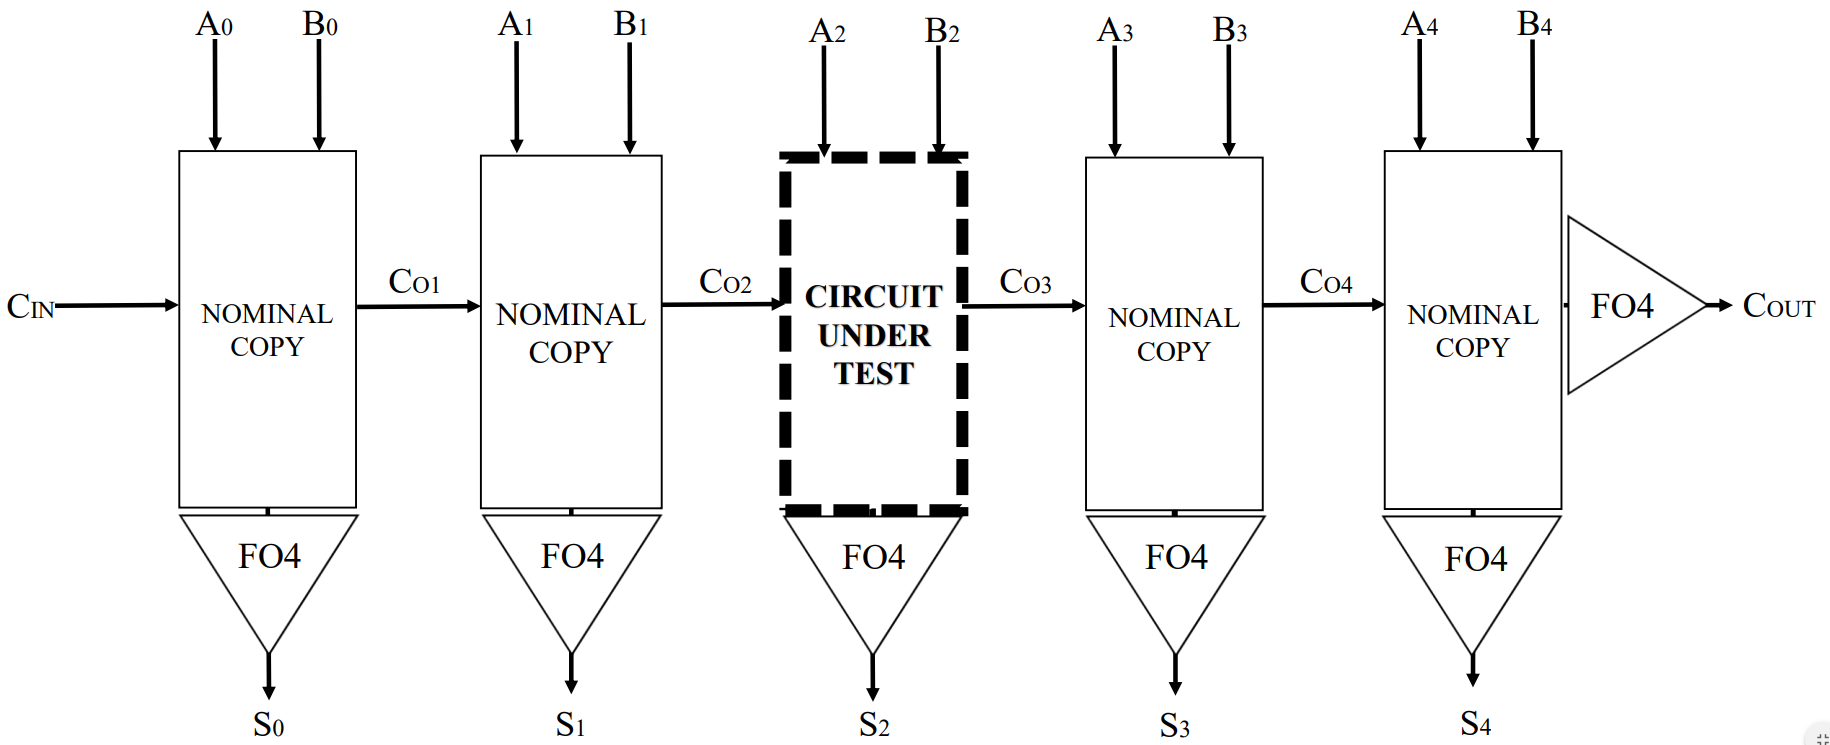
\includegraphics[width=\textwidth, trim={0cm 0cm 0cm 0cm},clip]{testbenchFA.png}
\caption{Test Bench for the Full Adders simulation.}
\label{fig:tbFA}
\legend{Source: From the author.}
\end{figure}


\chapter{Results}
\section{Over robustness enhancing circuits}
 Over all simulations there were non-viable scenarios. Such scenarios kept clustered around the supply voltages of 0.1V, over any scenario above 3\% WFF, and 0.2V, over scenarios above 4\% WFF for the inverter, ST and SIG. The TIST results presented a discrepancy in relation to the aforementioned designs. For the TIST designs at 2 to 1 and 3 to 1 proportions, the 0.1V scenarios at above 2\% WFF level are not viable. For 0.2V and 0.3V the 3 to 1 designs only presented viable scenarios at 1\% WFF while the 2 to 1 proportion designs did not operate properly at such supply voltage at any variability level. For the 0.4V the 3 to 1 and 2 to 1 designs worked at below 3\% and 2\% WFF levels, respectively. For 0.5V the 3 to 1 and 2 to 1 designs worked at below 5\% and 3\% WFF levels, respectively. Finally, at 0.6V and 0.7V, all scenarios worked properly.

 Given so, in overall, each design presented non-viable scenarios at below threshold voltages, with the TIST layouts presenting a much higher number of failures only working properly, at all variability levels, on 0.6V and 0.7V supply voltages. This results shows the lower robustness and more complex way of sizing for the TIST, which may not be advised for critical applications. All scenarios frequencies are shown in Table \ref{tab:freqs}.

 On average, the ST, SIG and TIST (2:1) operated at around half the inverter's frequency (47.61\%, 50.5\% and 49.71\% respectively) while the TIST (3:1) worked at 65.72\% of the inverter frequency. This is expected since their input capacitance is much higher, from a two-transistor design to a six-transistor design and, for the ST and TIST designs, the hysteresis keeps the output from switching much longer than in the other considered designs. The 3:1 TIST designs present a higher frequency, in comparison to its 2 to 1 proportion counterpart, given the higher proportion giving less resistance and higher currents to the circuit, making it faster in charging and discharging its nodes and output.

Considering the impact of variability on the frequency retention, in comparison to a low variability scenario (1\% WFF) the inverter, ST, SIG, TIST 2:1 and TIST 3:1 presented up to 40.03\%, 48.81\%, 48.20\%, 59.4\%, and 53.17\% average decrease on frequencies considering the worst case scenario, respectively. It is important to elucidate that in order to not deflate the decrease results of the TIST designs due to the large number of non-viable scenarios, the results were calculated considering such scenarios to work at 0Hz, as shown in Fig. \ref{fig:freqRetWFF}.

\begin{figure}[]
\centering
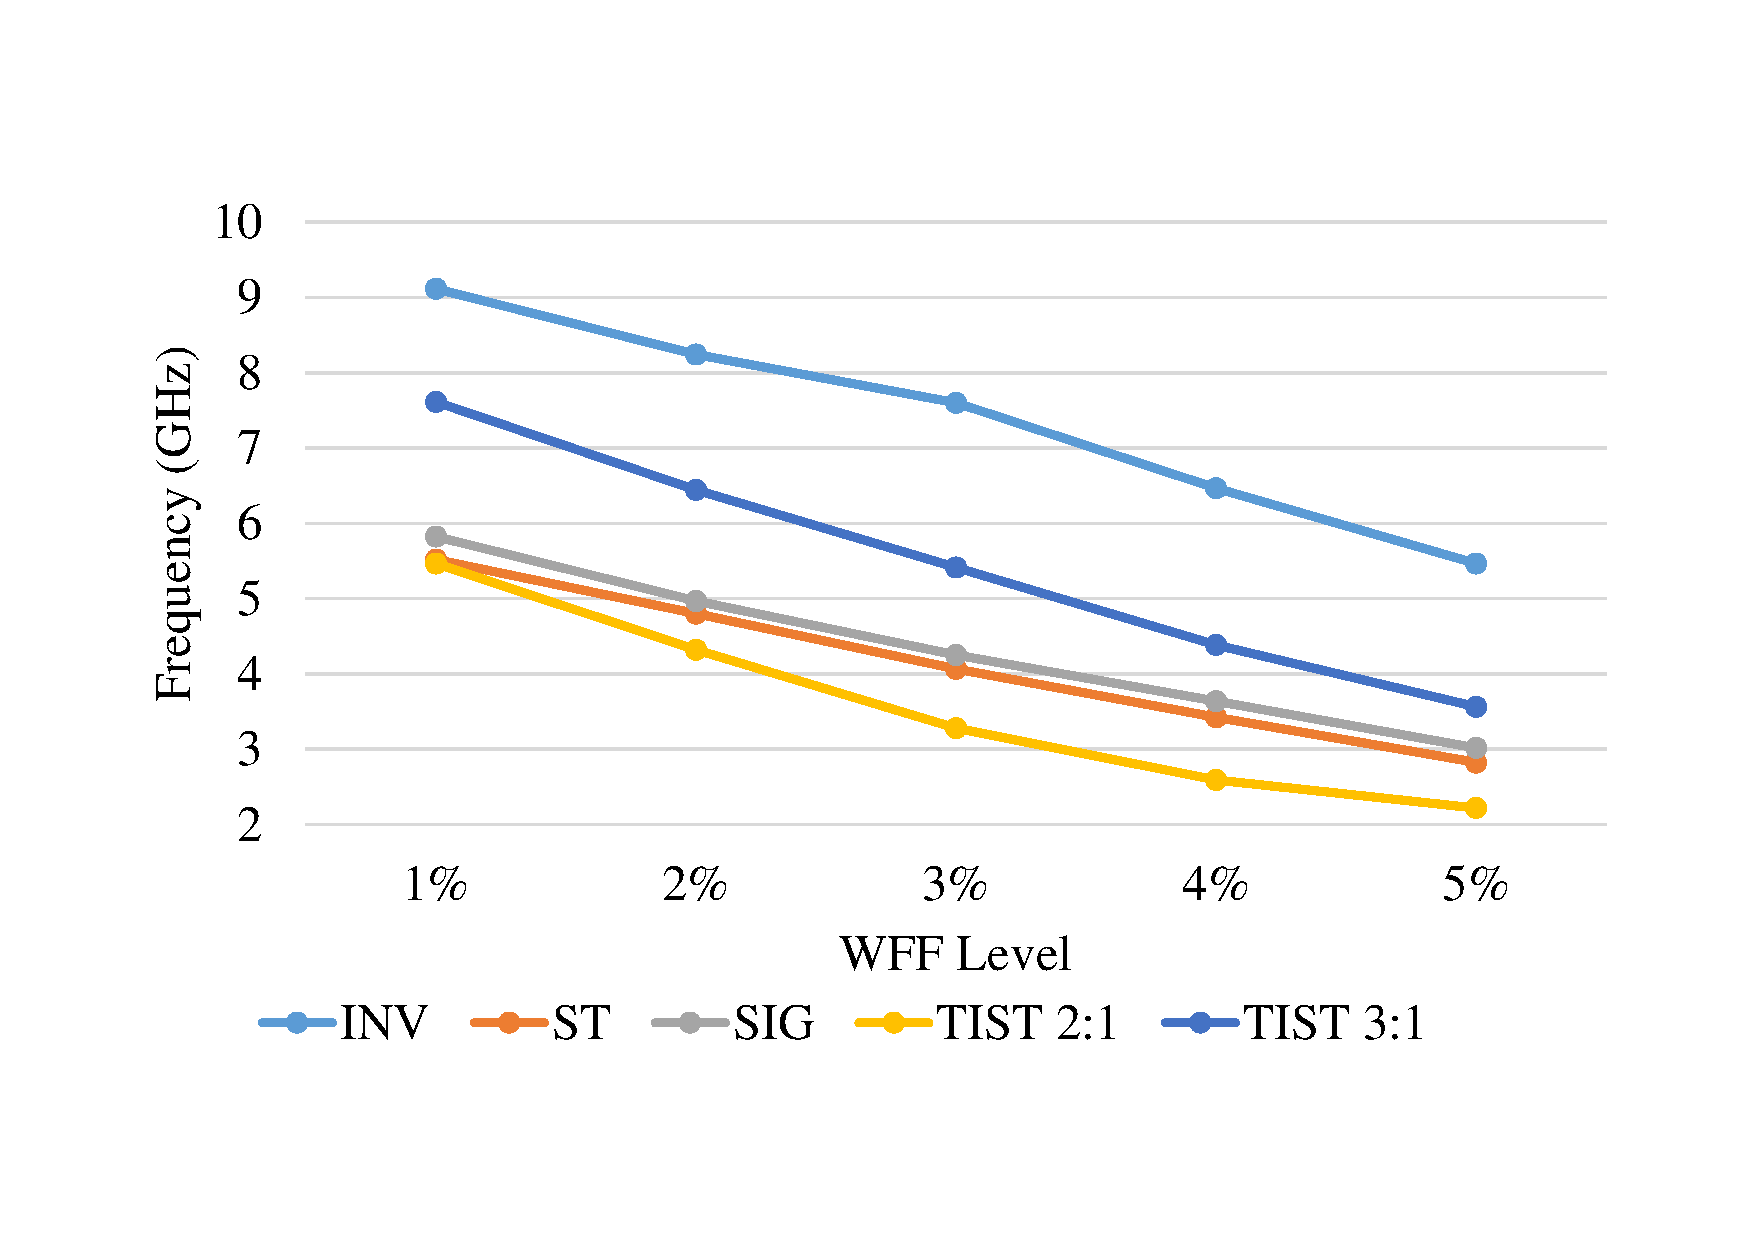
\includegraphics[width=\textwidth, trim={2cm 3cm 2cm 3cm},clip]{freqRetWFF.pdf}
\caption{Frequency decrease over variability scaling for each design.}
\label{fig:freqRetWFF}
\legend{Source: From the author.}
\end{figure}

%\begin{comment}
%\begin{figure}[H]
%\centering
%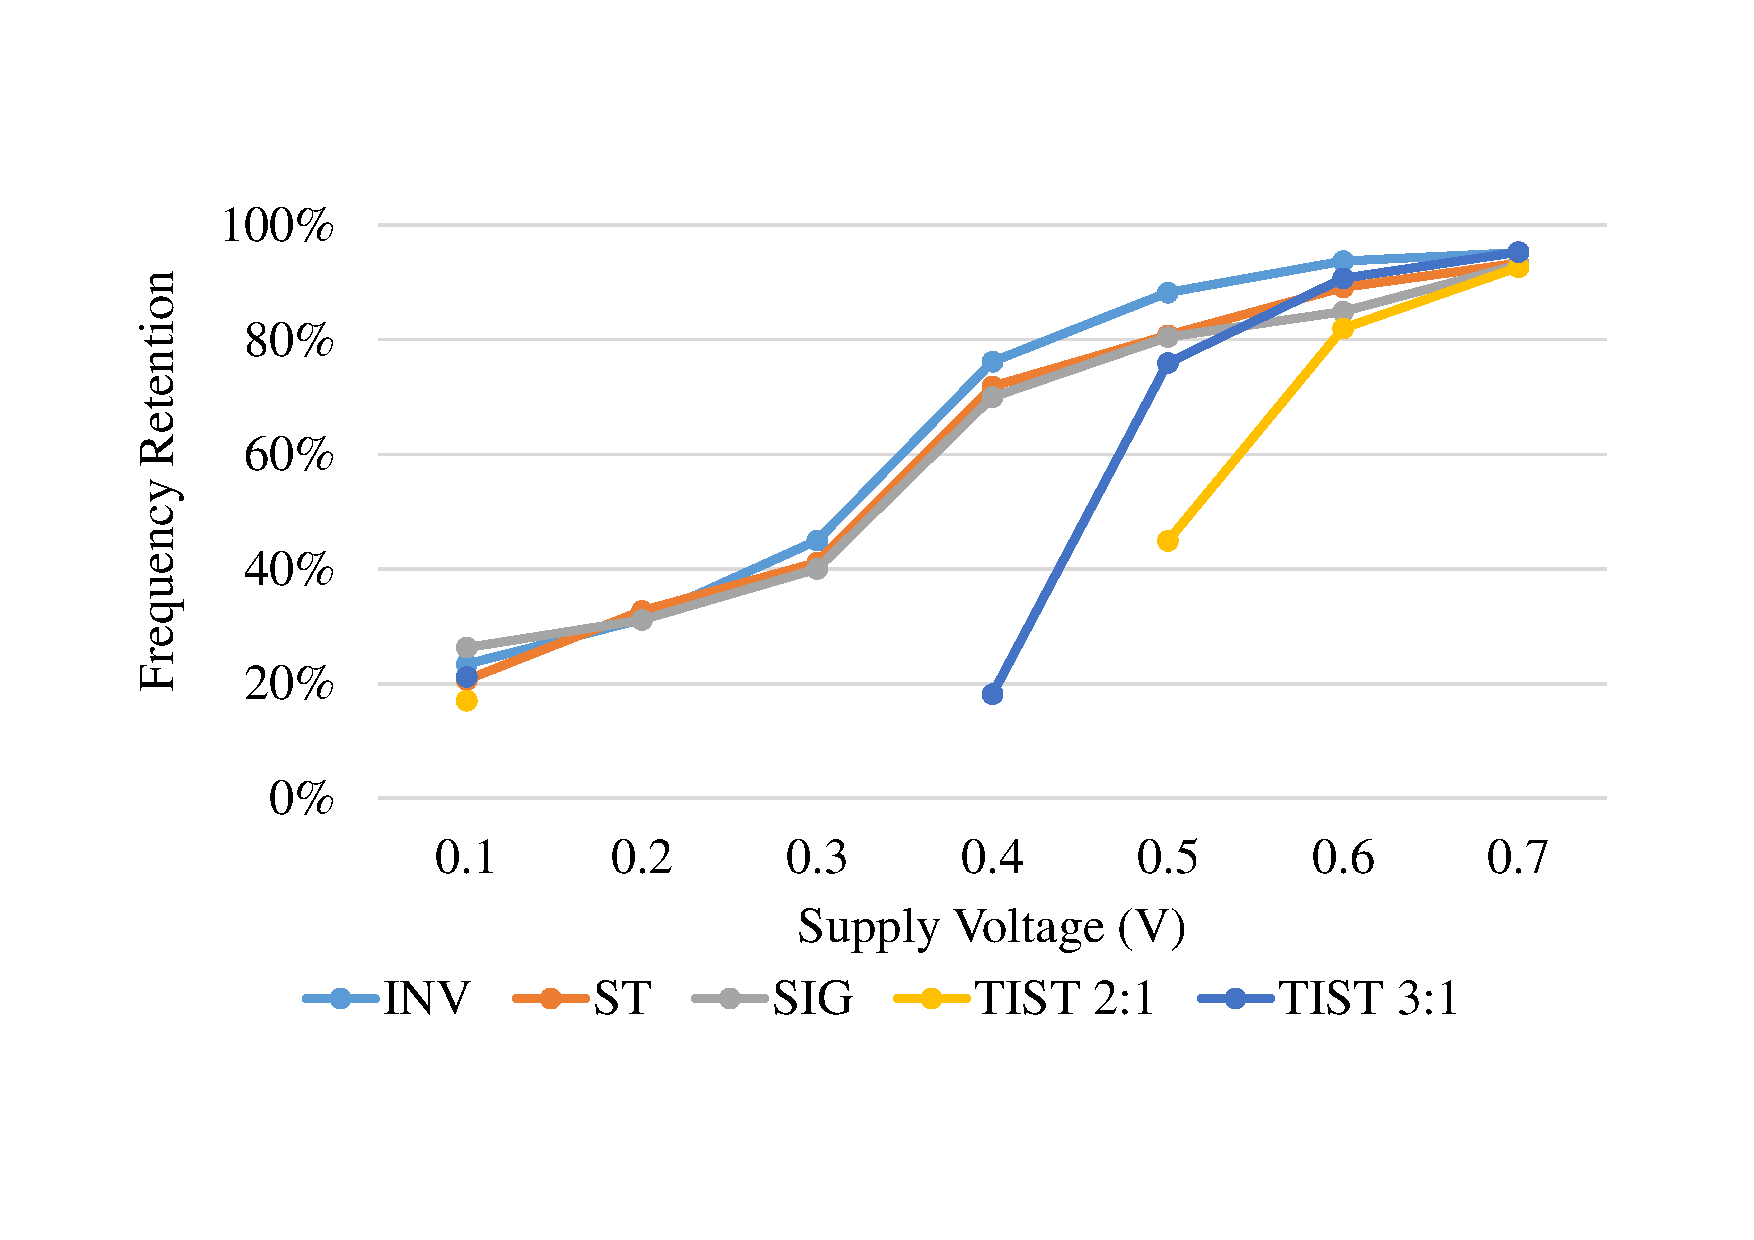
\includegraphics[width=0.8\textwidth, trim={2cm 3.5cm 2cm 3cm},clip]{freqRet2.pdf}
%\caption{Frequency retention rates for the 2\% WFF scenarios.}
%\label{fig:freqRet2}
%\legend{Source: From the author.}
%\end{figure}

%\begin{figure}[H]
%\centering
%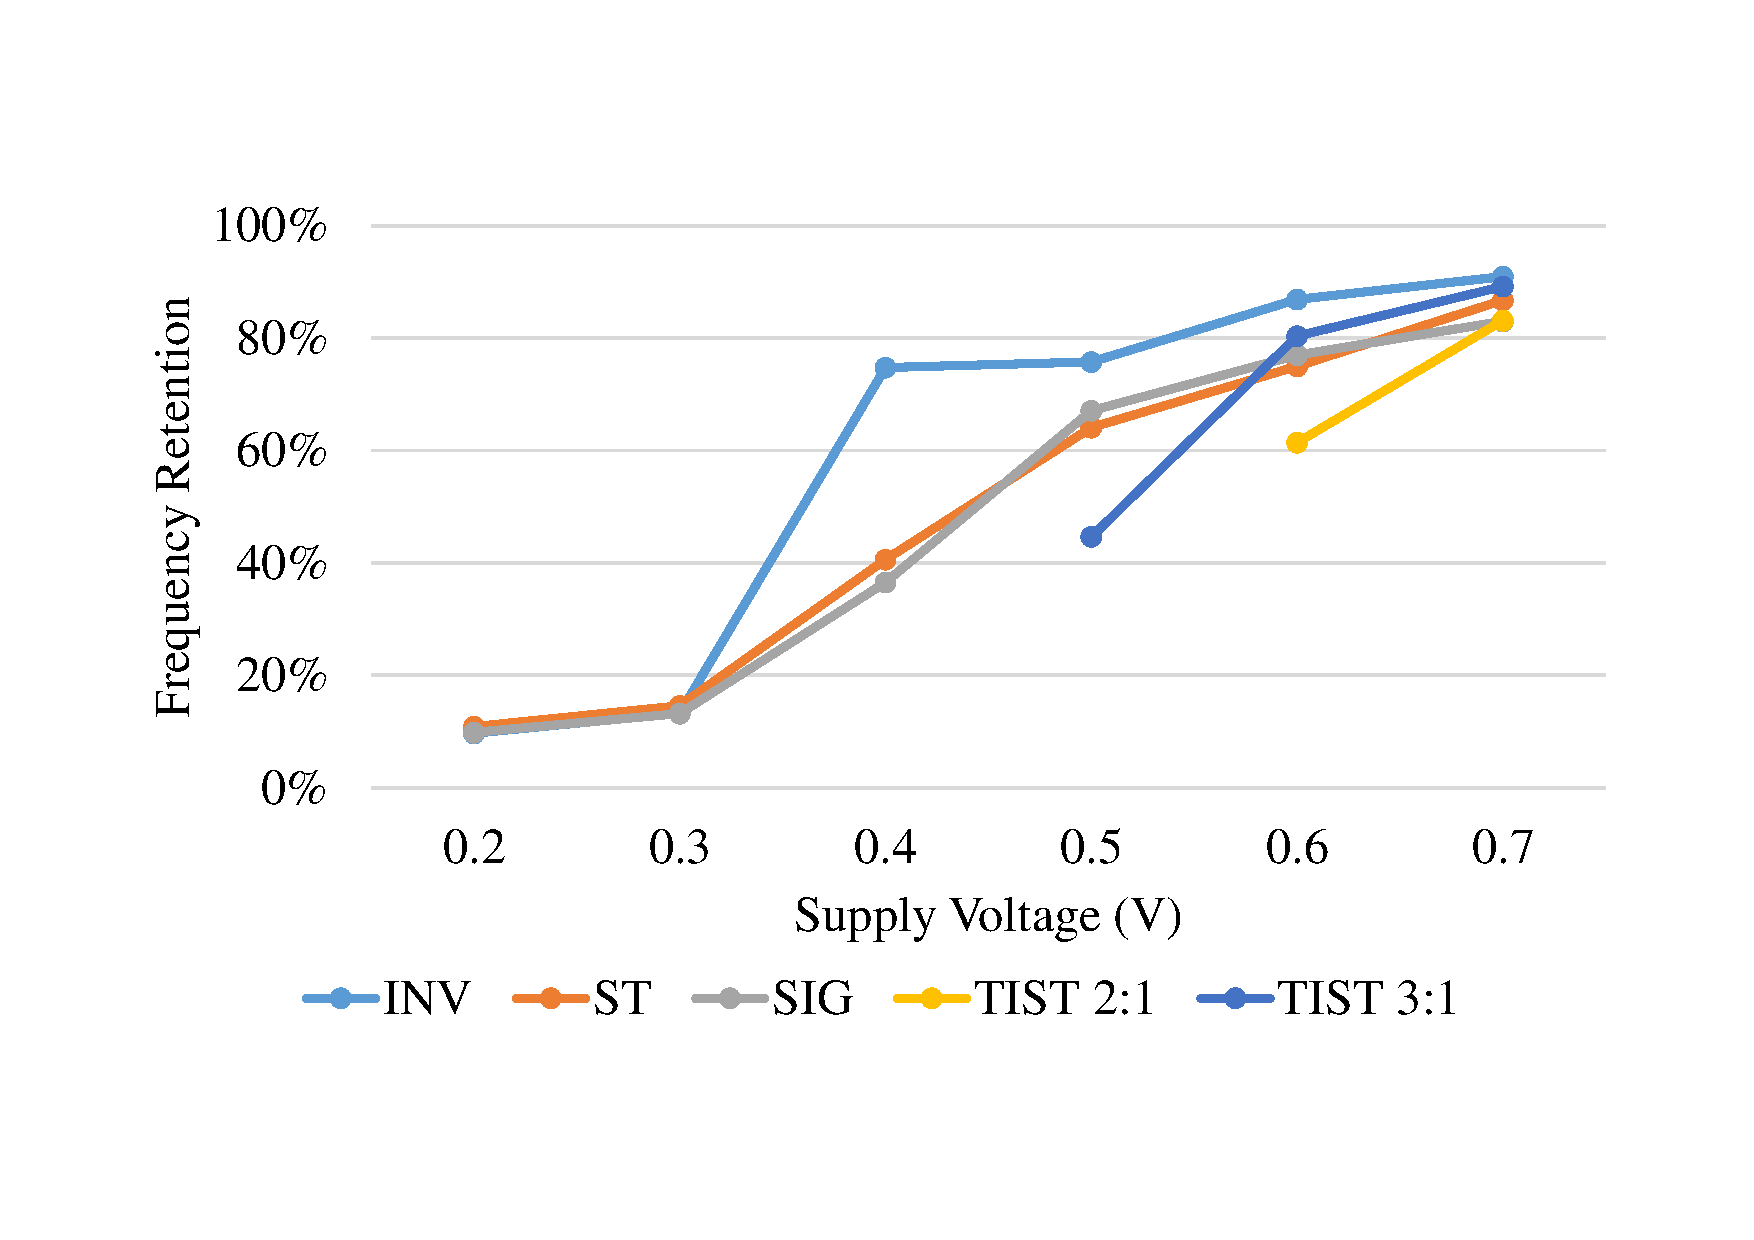
\includegraphics[width=0.8\textwidth, trim={2cm 3.5cm 2cm 3cm},clip]{freqRet3.pdf}
%\caption{Frequency retention rates for the 3\% WFF scenarios.}
%\label{fig:freqRet3}
%\legend{Source: From the author.}
%\end{figure}

%\begin{figure}[H]
%\centering
%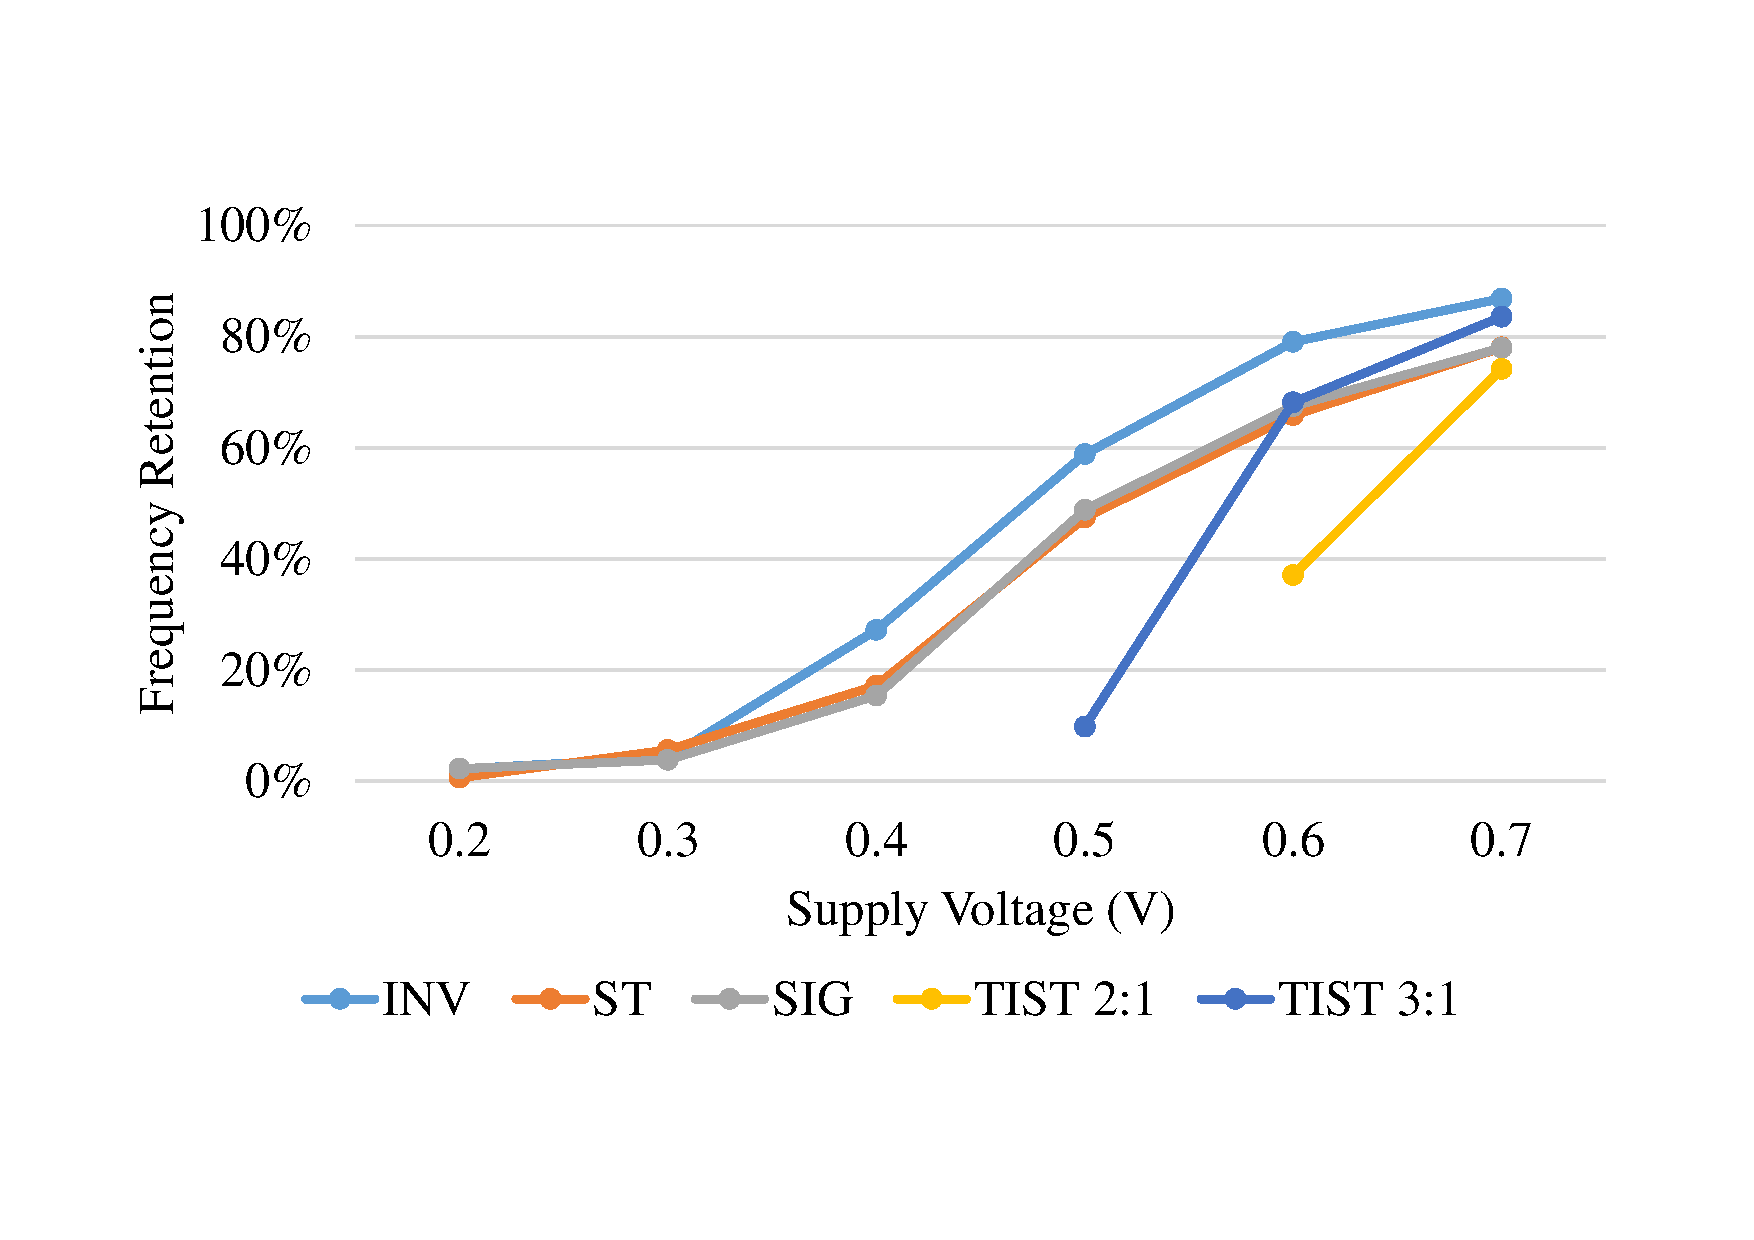
\includegraphics[width=0.8\textwidth, trim={2cm 3.5cm 2cm 3cm},clip]{freqRet4.pdf}
%\caption{Frequency retention rates for the 4\% WFF scenarios.}
%\label{fig:freqRet4}
%\legend{Source: From the author.}
%\end{figure}

%\begin{figure}[H]
%\centering
%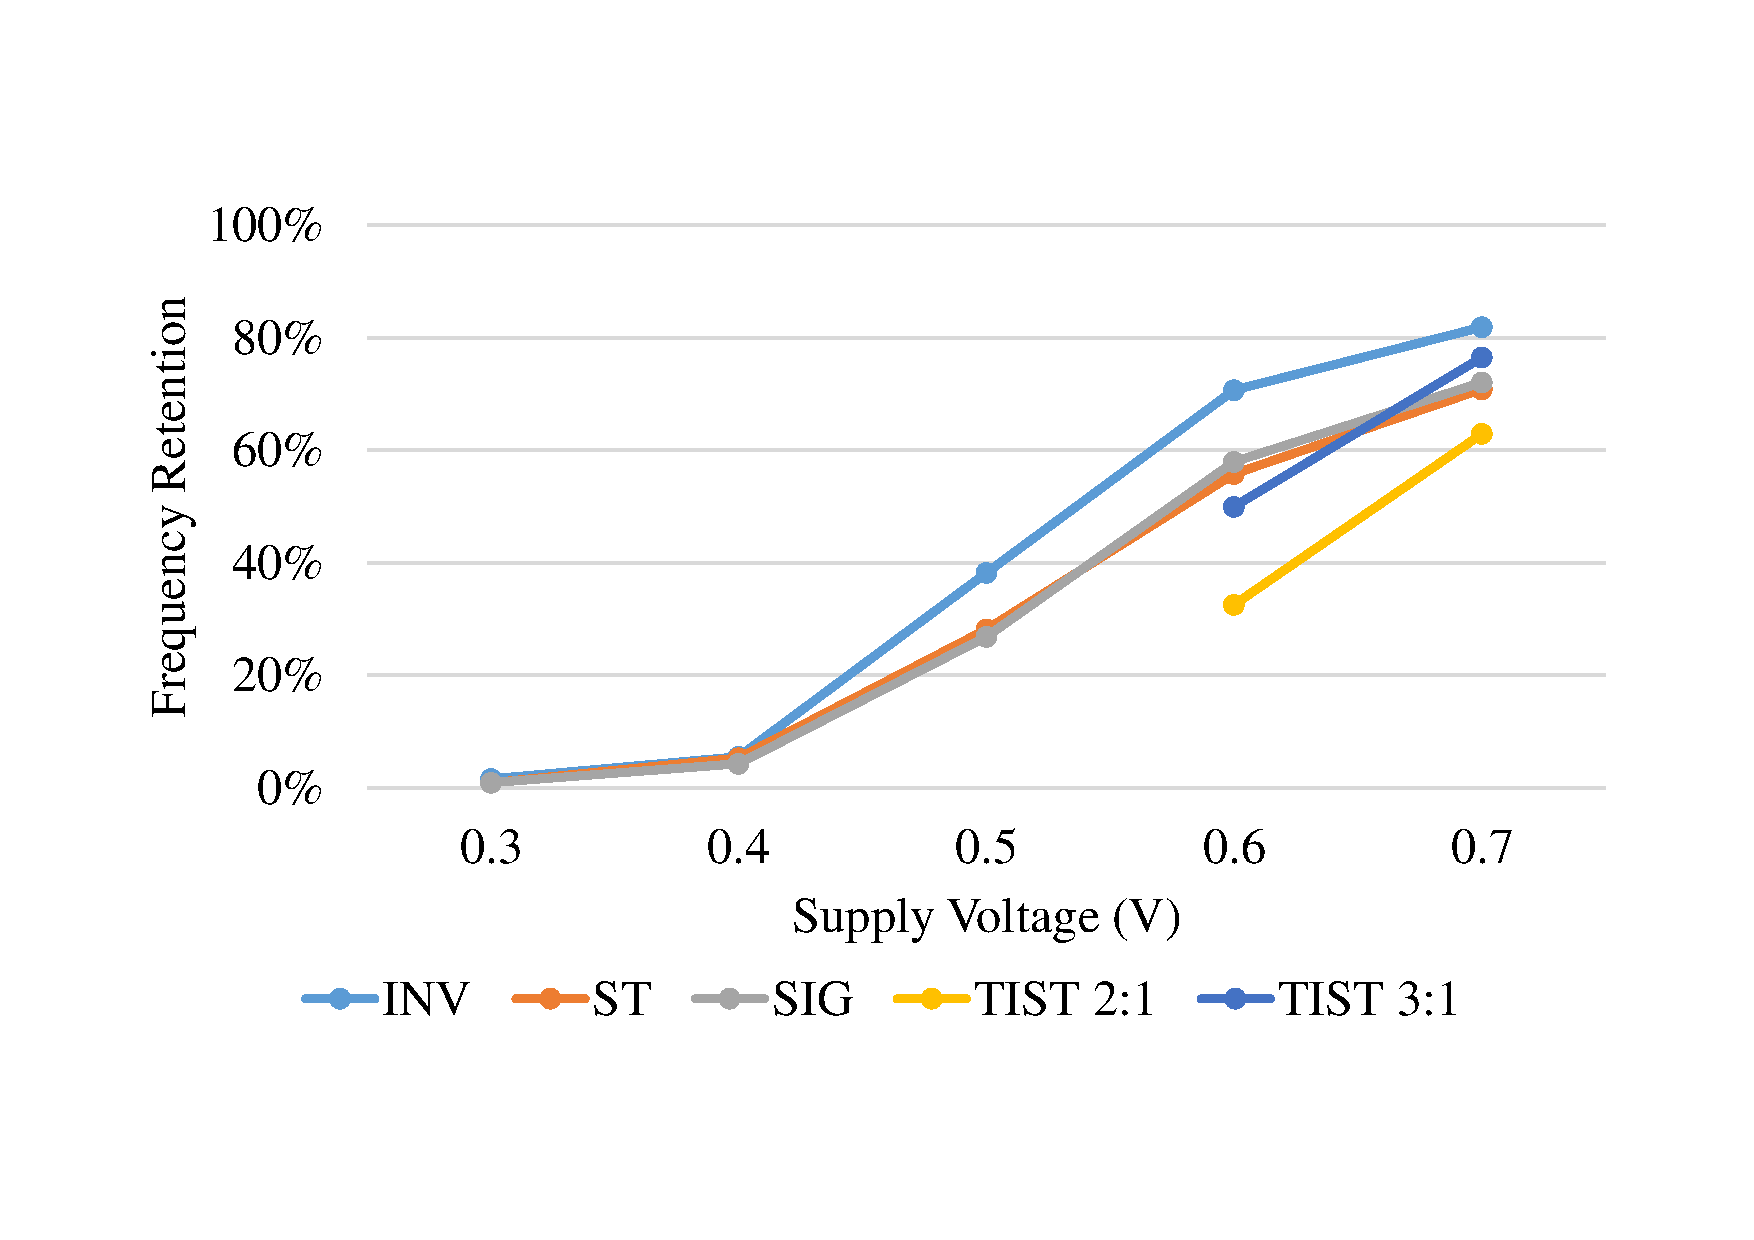
\includegraphics[width=0.8\textwidth, trim={2cm 3.5cm 2cm 3cm},clip]{freqRet5.pdf}
%\caption{Frequency retention rates for the 5\% WFF scenarios.}
%\label{fig:freqRet5}
%\legend{Source: From the author.}
%\end{figure}
%\end{comment}

Such performance degradation is expected since process variability will, in many cases, increase the transistors $V_{TH}$, making necessary to decrease the circuits frequency to work properly. Alongside, in higher transistor count circuits, it is expected a higher impact since the variability effect on transistors will work as a chain reaction, with the previous node own deviation accumulating along the next circuit nodes and so on, until the output node. Given that, it is expected for the ST and SIG to present a higher impact due to the inserted process variability. The TIST present higher decreases due to their higher number of non-viable scenarios.  %Although, the small difference between the inverter and the robustness enhancing designs, shows that the inverter has higher susceptibility to the process variability impact.

\begin{table}[]
\centering
\caption{All scenarios frequencies.}
\label{tab:freqs}
\resizebox{\textwidth}{!}{
\begin{tabular}{|c|c|c|c|c|c|c|c|c|}
\hline
\multirow{2}{*}{Design} & \multirow{2}{*}{WFF} & \multicolumn{7}{c|}{Supply Voltage (V)}                             \\ \cline{3-9}
                        &                      & 0.1     & 0.2     & 0.3     & 0.4     & 0.5     & 0.6     & 0.7     \\ \hline
\multirow{5}{*}{INV}    & 1\%                  & 2.18MHz & 49.4MHz & 1.12GHz & 6.5GHz  & 13.6GHz & 19.1GHz & 23.4GHz \\ \cline{2-9}
                        & 2\%                  & 510KHz  & 15.4MHz & 504MHz  & 4.95GHz & 12GHz   & 17.9GHz & 22.3GHz \\ \cline{2-9}
                        & 3\%                  & -       & 4.79MHz & 149MHz  & 4.86GHz & 10.3GHz & 16.6GHz & 21.3GHz \\ \cline{2-9}
                        & 4\%                  & -       & -       & 47.2MHz & 1.77GHz & 8GHz    & 15.1GHz & 20.3GHz \\ \cline{2-9}
                        & 5\%                  & -       & -       & 17.8MHz & 360MHz  & 5.2GHz  & 13.5GHz & 19.2GHz \\ \hline
\multirow{5}{*}{ST}     & 1\%                  & 930KHz  & 22MHz   & 510MHz  & 3.2GHz  & 7.8GHz  & 12GHz   & 15.1GHz \\ \cline{2-9}
                        & 2\%                  & 192KHz  & 7.2MHz  & 210MHz  & 2.3GHz  & 6.3GHz  & 10.7GHz & 14.1GHz \\ \cline{2-9}
                        & 3\%                  & -       & 2.39MHz & 74.2MHz & 1.3GHz  & 5GHz    & 9GHz    & 13.1GHz \\ \cline{2-9}
                        & 4\%                  & -       & -       & 28.4MHz & 550MHz  & 3.7GHz  & 7.9GHz  & 1.11GHz \\ \cline{2-9}
                        & 5\%                  & -       & -       & 4.6MHz  & 170MHz  & 2.2GHz  & 6.7GHz  & 10.7GHz \\ \hline
\multirow{5}{*}{SIG}    & 1\%                  & 1.02MHz & 23.8MHz & 540MHz  & 3.5GHz  & 8.2GHz  & 12.6GHz & 15.9GHz \\ \cline{2-9}
                        & 2\%                  & 268KHz  & 7.4MHz  & 216MHz  & 2.45GHz & 6.6GHz  & 10.7GHz & 14.8GHz \\ \cline{2-9}
                        & 3\%                  & -       & 2.34MHz & 71.4MHz & 1.25GHz & 5.5GHz  & 9.7GHz  & 13.2GHz \\ \cline{2-9}
                        & 4\%                  & -       & -       & 20.8MHz & 540MHz  & 4GHz    & 8.5GHz  & 12.4GHz \\ \cline{2-9}
                        & 5\%                  & -       & -       & 5MHz    & 150MHz  & 2.2GHz  & 7.3GHz  & 11.5GHz \\ \hline
\multirow{5}{*}{\begin{tabular}[c]{@{}c@{}}TIST\\ 2:1\end{tabular}} & 1\% & 833KHz & -      & -      & 783MHz & 6.37GHz & 13.3GHz & 17.8GHz \\ \cline{2-9}
                        & 2\%                  & 142KHz  & -       & -       & -       & 2.86GHz & 10.9GHz & 16.5GHz \\ \cline{2-9}
                        & 3\%                  & -       & -       & -       & -       & -       & 8.17GHz & 14.8GHz \\ \cline{2-9}
                        & 4\%                  & -       & -       & -       & -       & -       & 4.93GHz & 13.2GHz \\ \cline{2-9}
                        & 5\%                  & -       & -       & -       & -       & -       & 4.33GHz & 11.2GHz \\ \hline
\multirow{5}{*}{\begin{tabular}[c]{@{}c@{}}TIST\\ 3:1\end{tabular}} & 1\% & 1.3MHz & 5.5MHz & 175MHz & 3.3GHz & 11.2GHz & 17.3GHz & 21.3GHz \\ \cline{2-9}
                        & 2\%                  & 275KHz  & -       & -       & 600MHz  & 8.51GHz & 15.7GHz & 20.3GHz \\ \cline{2-9}
                        & 3\%                  & -       & -       & -       & -       & 5GHz    & 13.9GHz & 19GHz   \\ \cline{2-9}
                        & 4\%                  & -       & -       & -       & -       & 1.1GHz  & 11.8GHz & 17.8GHz \\ \cline{2-9}
                        & 5\%                  & -       & -       & -       & -       & -       & 8.65GHz & 16.3GHz \\ \hline
\end{tabular}
}
\end{table}

Given the propagation time deviations for each design, in comparison to the inverter, and considering all scenarios, the ST and SIG presented 36.36\% and 43.21\% lower sensibility, respectively. While the TIST with 2:1 and 3:1 proportions presented 72.89\% and 103.26\% higher deviations, respectively, as shown in Fig. \ref{fig:delaysDev}. When considering only scenarios where all designs worked properly, the ST and SIG presented small increases of 8.54\% and 7.04\% in sensibility, with the TIST 2:1 and 3:1 presenting 146.15\% and 36.28\% higher sensibility.

    \begin{figure}[]
        \centering
            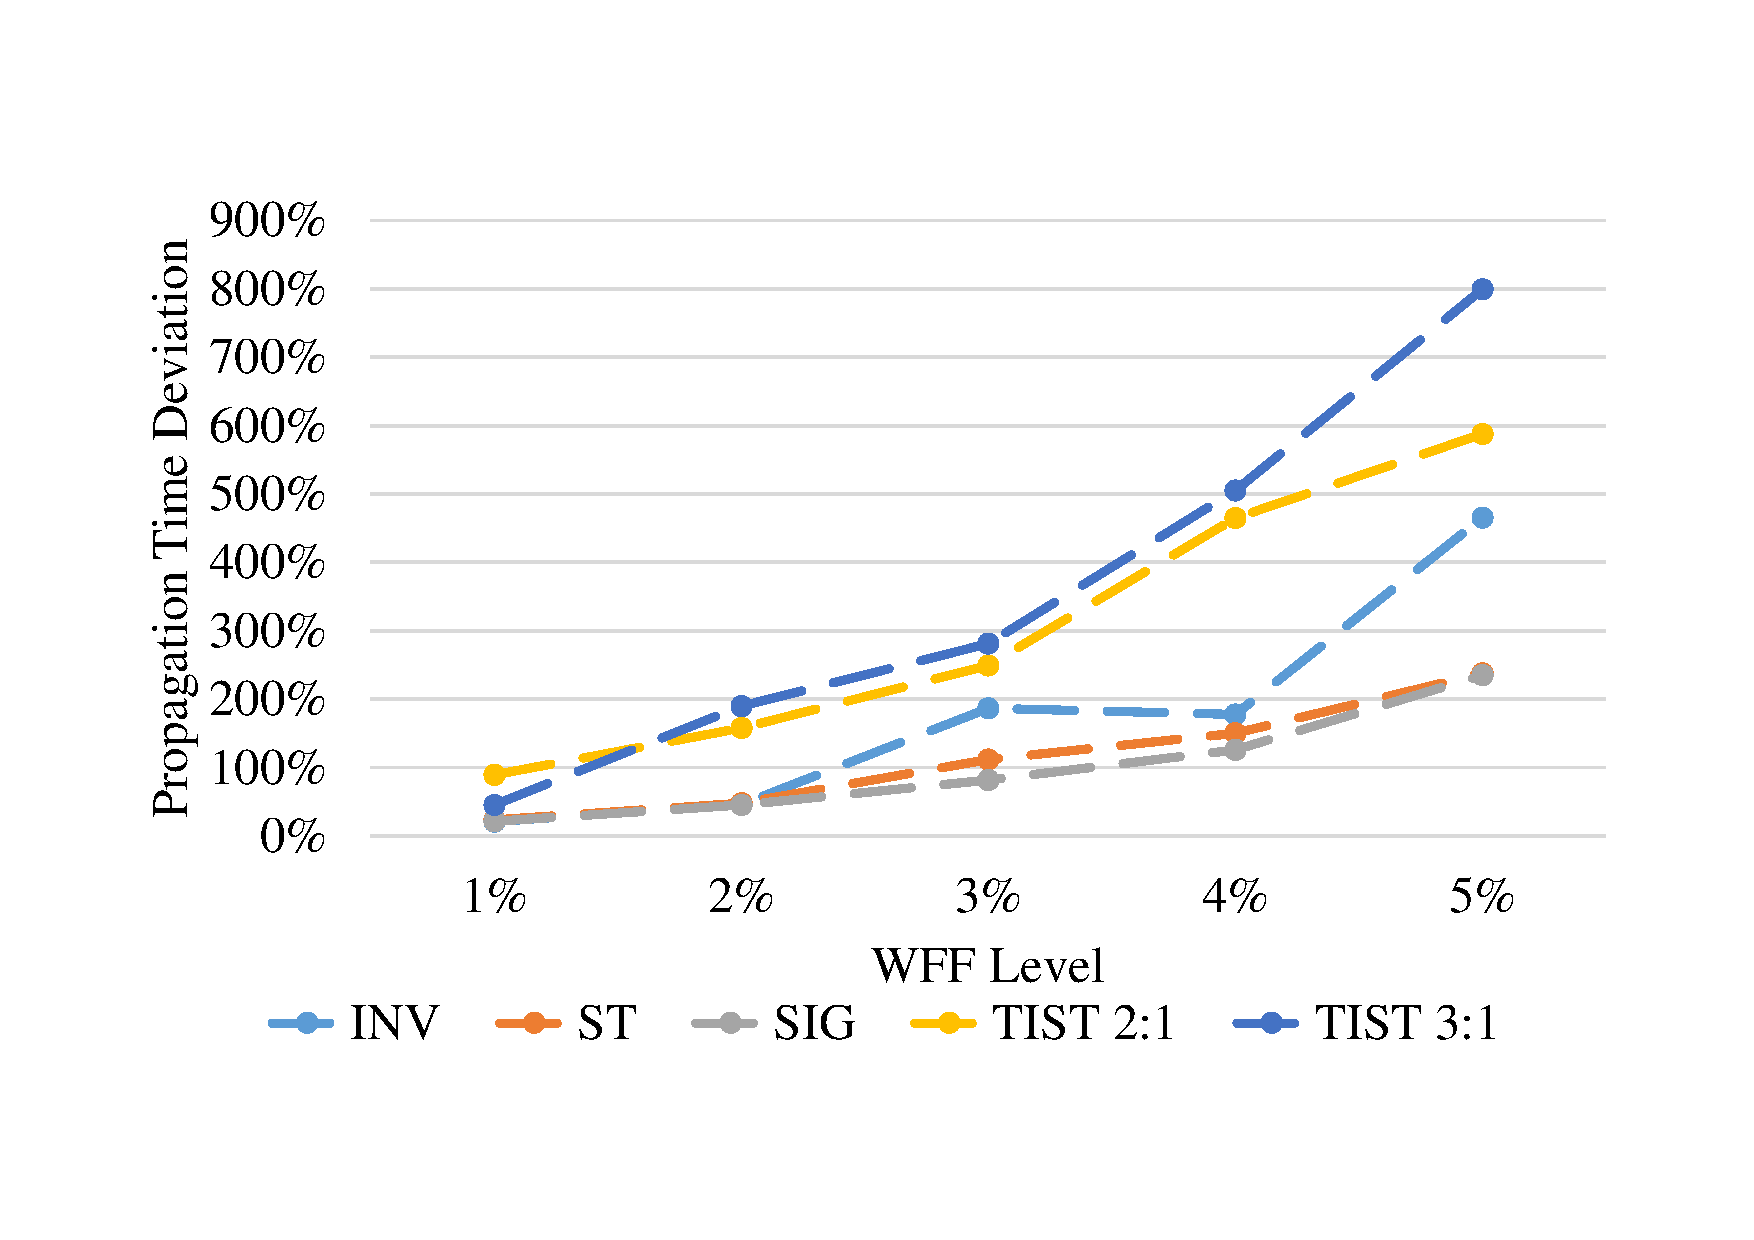
\includegraphics[width=\textwidth, trim={2cm 3cm 2cm 3cm}, clip]{delayDevWFF.pdf}
            \caption{Propagation times deviation for each design in relation to the WFF level considering all scenarios.}
        \label{fig:delaysDev}
        \legend{Source: From the author.}
    \end{figure}

\section{Energy Consumption and Deviation}
    Concerning energy consumption absolute values, the ST, SIG, TIST 2:1 and, TIST 3:1 presented on average, 173.07\%, 50.74\%, 480.68\% and, 310.83\% higher consumption compared to the traditional inverter. This is mainly related to the transistor count difference between all designs, and the inverter. The ST higher consumption is justified due to the dependency of its feedback mechanism on the output value in contrast to the SIG feed-forward mechanism being directly dependent on the input value. The dependency over the output value of the ST makes it slower, hence the output dependency over the input itself and the input capacitance, increasing the energy consumption. The difference between different proportions of TIST designs is mainly due to lower frequencies on high variability scenarios for the 2 to 1 designs. The designs with a 2:1 proportion presented up to 40.94\% lower frequency in comparison to its 3 to 1 proportion counterparts. Additionally, the higher energy consumption for TIST designs is mainly due to the 6 (3 to the ground and 3 to the source) total paths enabling the circuit to charge/discharge with no mechanism for the minimization of the leakage power.

    The energy consumption increase over each variability scenario kept stable over 15.16\%, 35.6\%, 20.94\%, 9.04\% and, 7.18\% for the inverter, ST, SIG, TIST 2:1 and, TIST 3:1, respectively. Such increase is related to the frequency decrease over variability scaling. The low increase related to the TIST designs is due to many of the low supply voltage scenarios not being taken into account, in comparison to the other designs, since it did not work properly. A more fair analysis would consider only the subset of cases where all designs worked properly. Given such subset, the energy increase over each variability scenario would be 17.59\%, 18.16\%, 18.62\%, 9.04\% and 11.59\% for the inverter, ST, SIG, TIST 2:1 and, TIST 3:1, respectively.
    %Energy consumption measures over variability scenarios for each design is shown at Figure \ref{figEnergiaAbs}.



    Concerning robustness, the ST and SIG presented a 55.83\%, 47.15\% higher sensibility while the TIST 2:1 and 3:1 presented a 42.39\% and 52.03\% lower sensibility to the process variability impact in comparison to the traditional inverter considering the scenarios where each design presented acceptable behavior. In order to make a fair comparison, considering only the subset of scenarios where all designs worked properly, the ST and TIST 3:1 presented 1.13\% and 33.36\% lower sensibilities while the SIG and TIST 2:1 presented 5.5\% and 7.99\% higher variability sensibility. Additionally, considering all cases, even when the circuit did not work properly, the ST, SIG, TIST 2:1, and TIST 3:1 presented 19.85\%, 12.09\%, 145.96\%, and 118.24\% higher sensibilities in comparison to the traditional inverter.
    %Which, as stated before, is expected.

    %\begin{figure}[b]
    %    \centering
    %        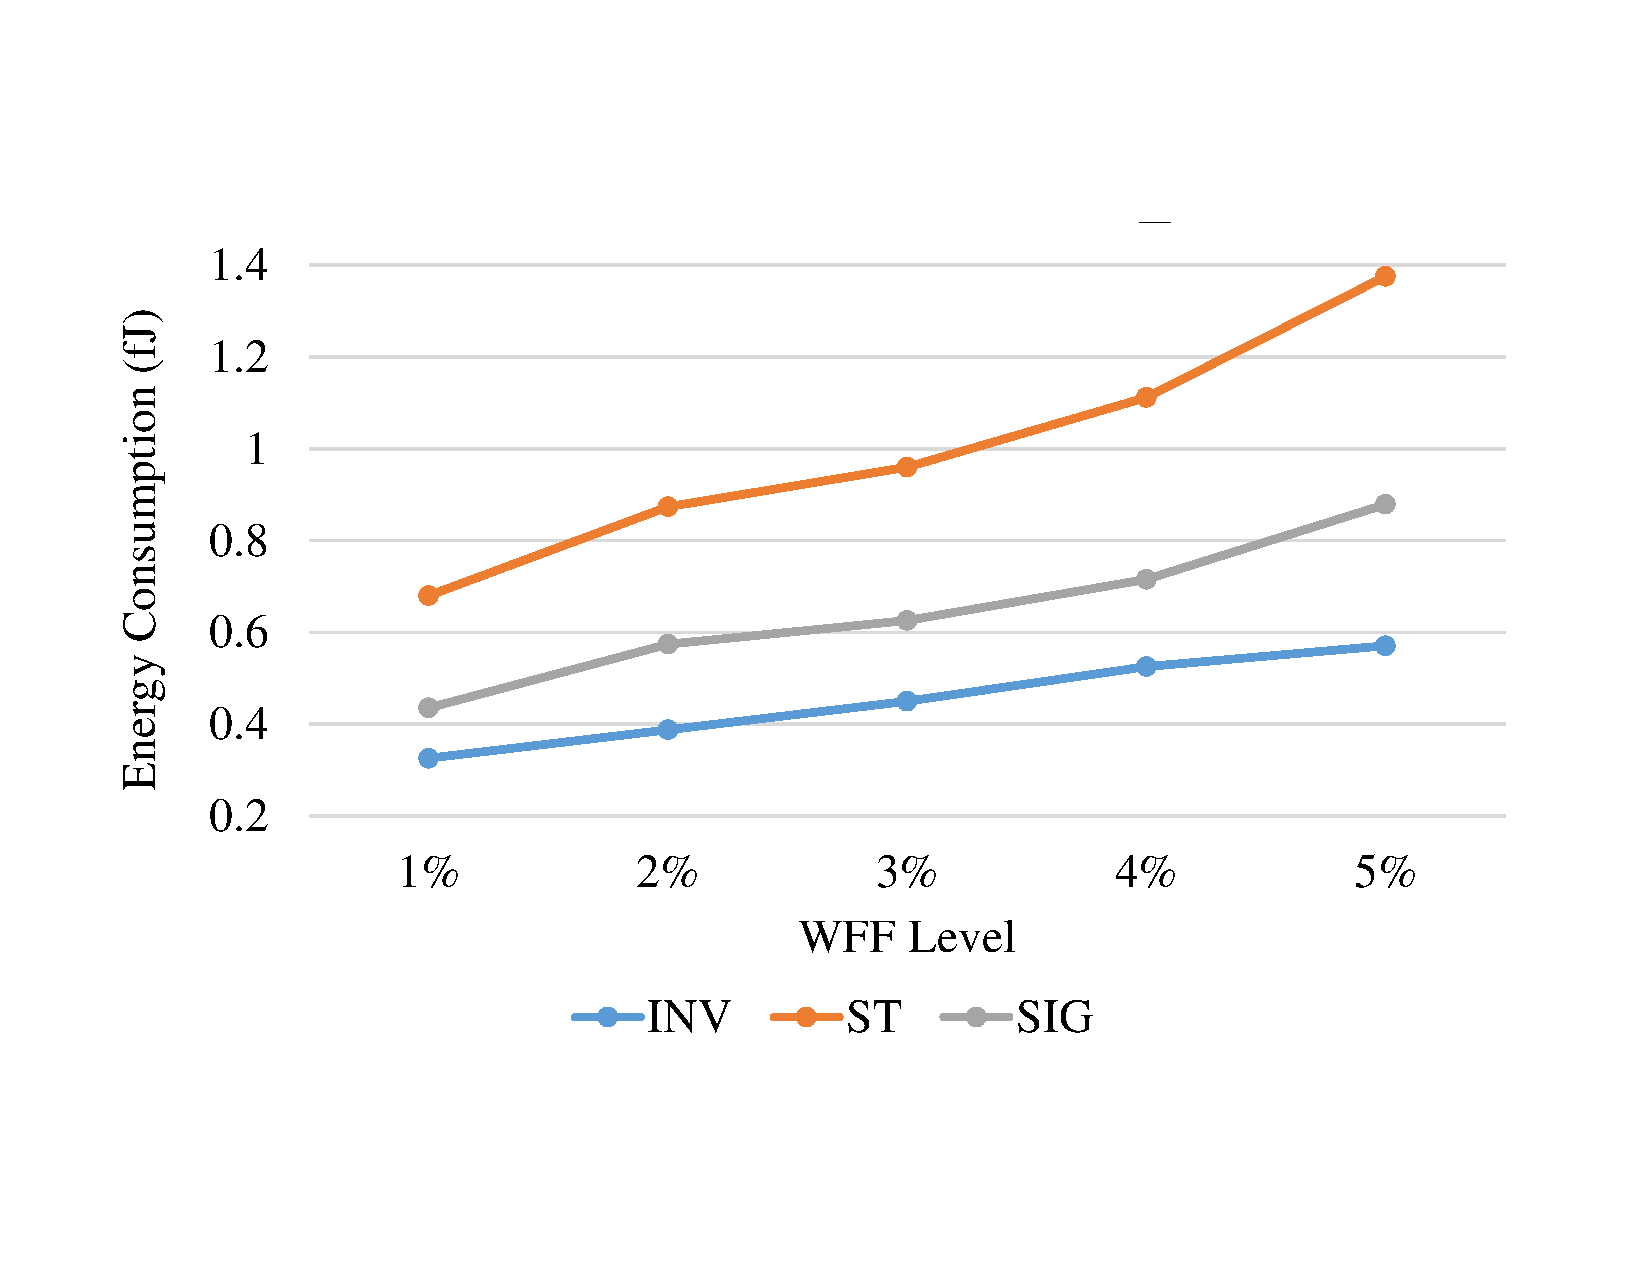
\includegraphics[width=0.45\textwidth, trim={2cm 4cm 2cm 4cm}, clip]{compEnergiaAbs.pdf}
            %\caption{Energy consumption increase over variability scaling.}
   %     \label{figEnergiaAbs}
  %  \end{figure}



    Three types of analysis were performed to identify the most appropriate layout depending on the scenario: 1) layout with the lowest energy consumption, 2) highest robustness and 3) the most Cost-Benefit (CB) oriented layout. The lowest energy layout is identified through the energy measures. The higher robustness layout is identified by the lowest normalized standard deviation concerning energy consumption and the CB layout is identified by the lowest value considering the product between the energy consumption and normalized standard deviation (EDP - Energy Deviation Product). The results are shown at Table \ref{tab:3types}.

    % Please add the following required packages to your document preamble:
% \usepackage{multirow}
% \usepackage{graphicx}



% Please add the following required packages to your document preamble:
% \usepackage{multirow}
\begin{table}[]
\centering
\caption{Recommended layout and supply voltage for each design and variability level.}
\label{tab:3types}
\resizebox{\textwidth}{!}{
\begin{tabular}{|c|c|c|c|c|c|c|c|}
\hline
\multirow{2}{*}{Design} & \multirow{2}{*}{WFF} & \multicolumn{2}{c|}{Minimum Energy} & \multicolumn{2}{c|}{Highest Robustness} & \multicolumn{2}{c|}{CB} \\ \cline{3-8}
                          &     & Supply (V) & \#Fins & Supply (V) & \#Fins       & Supply (V) & \#Fins \\ \hline
\multirow{5}{*}{INV}      & 1\% & 0.1        & 1 or 2 & 0.7        & 1            & 0.7        & 1      \\ \cline{2-8}
                          & 2\% & 0.1        & 1      & 0.3        & 4 or 5       & 0.2        & 2 to 4 \\ \cline{2-8}
                          & 3\% & 0.2        & 1      & 0.3        & 5            & 0.3        & 3 to 5 \\ \cline{2-8}
                          & 4\% & 0.3        & 1 or 2 & 0.4        & 5            & 0.4        & 5      \\ \cline{2-8}
                          & 5\% & 0.3        & 1      & 0.4        & 1       & 0.4        & 1      \\ \hline
\multirow{5}{*}{ST}       & 1\% & 0.1        & 1      & 0.7        & 5            & 0.7        & 1      \\ \cline{2-8}
                          & 2\% & 0.2        & 1      & 0.7        & 5            & 0.7        & 1      \\ \cline{2-8}
                          & 3\% & 0.2        & 1      & 0.7        & 4 or 5       & 0.3        & 1      \\ \cline{2-8}
                          & 4\% & 0.3        & 1      & 0.4        & 2            & 0.4        & 1 or 2 \\ \cline{2-8}
                          & 5\% & 0.4        & 1      & 0.5        & 2 to 5       & 0.5        & 1 or 2 \\ \hline
\multirow{5}{*}{SIG}      & 1\% & 0.1        & 1      & 0.7        & 2            & 0.7        & 1      \\ \cline{2-8}
                          & 2\% & 0.2        & 1      & 0.3        & 3 or 4       & 0.7        & 1      \\ \cline{2-8}
                          & 3\% & 0.2        & 1      & 0.3        & 3            & 0.3        & 1      \\ \cline{2-8}
                          & 4\% & 0.3        & 1      & 0.4        & 3            & 0.4        & 2 or 3 \\ \cline{2-8}
                          & 5\% & 0.4        & 1      & 0.5        & 2 or 3       & 0.5        & 2      \\ \hline
\multirow{5}{*}{TIST 2:1} & 1\% & 0.1        & 2F1F   & 0.7        & 4F2F         & 0.7        & 2F1F   \\ \cline{2-8}
                          & 2\% & 0.1        & 2F1F   & 0.6        & 4F2F         & 0.6        & 2F1F   \\ \cline{2-8}
                          & 3\% & 0.7        & 2F1F   & 0.6        & 2F1F         & 0.6        & 2F1F   \\ \cline{2-8}
                          & 4\% & 0.7        & 2F1F   & 0.7        & 4F2F         & 0.7        & 2F1F   \\ \cline{2-8}
                          & 5\% & 0.7        & 2F1F   & 0.7        & 6F3F         & 0.7        & 2F1F   \\ \hline
\multirow{5}{*}{TIST 3:1} & 1\% & 0.1        & 3F1F   & 0.7        & 6F2F         & 0.7        & 3F1F   \\ \cline{2-8}
                          & 2\% & 0.1        & 3F1F   & 0.7        & 6F2F or 3F1F & 0.7        & 3F1F   \\ \cline{2-8}
                          & 3\% & 0.7 or 0.6 & 3F1F   & 0.6 or 0.7 & 6F2F or 3F1F & 0.7        & 3F1F   \\ \cline{2-8}
                          & 4\% & 0.7 or 0.6 & 3F1F   & 0.6        & 6F2F         & 0.6        & 3F1F   \\ \cline{2-8}
                          & 5\% & 0.7 or 0.6 & 3F1F   & 0.6        & 3F1F         & 0.6        & 3F1F   \\ \hline
\end{tabular}
}
\end{table}

    Some results will show more than one appropriate layout/supply voltage. Values of energy consumption, energy normalized deviation and EDPs between the respective minimum value and, relatively, 5\% higher values were considered in order to provide more flexibility. It is possible to identify patterns concerning the minimum energy and highest robustness layouts. The minimum energy layouts contain only few fins and lower supply voltages. Both low values aim to lower currents and increase resistance, therefore decreasing energy consumption. As variability rises, the supply voltage rises as well. That is due to the lower frequencies applied in those scenarios and the consequent increase on propagation times, given that energy is the by-product of power and time. A higher supply voltage will decrease propagation times followed by a decrease on energy consumption. The TIST designs present a steep increase on supply voltage, from 0.1V to 0.6V/0.7V due to the lack of possible mid-term (0.2V to 0.5V) viable scenarios.

    The robust layouts present a shift on supply voltage. At saturation region, the on-current presents an exponential dependency over the $V_{TH}$, as shown in equation \ref{eqn:sat}, while at the linear region, the on-current presents a linear dependency over the $V_{TH}$, as shown in equation \ref{eqn:lin}. For both equations, the $I_{D,sat}$ is the saturation current, $I_{D,lin}$ is the linear current, $\mu_p$ is the p-material electron mobility, $C_{ox}$ is the specific capacitance of the gate, $W$ is the transistor width, $L$ is the transistor length, $V_{GS}$ is the gate-source voltage, $V_{DS}$ is the drain-source voltage, and $V_T$ is the threshold voltage. At low level variability scenarios, a saturation on-current will not present significant variations, while at high variability scenarios the on-current must fall to linear region in order to present lower deviations.

    %\begin{equation}
    %    \centering
    %    \label{eqn:somelabel}
    %    I_D = 0
    %    \begin{cases}
    %    V_{GS} > V_T
    %    \end{cases}
    %\end{equation}
%\begin{subequations}
    \begin{equation}
        \centering
        \label{eqn:sat}
        I_{D,sat} = \frac{\mu_p \cdot C_{ox}}{2} \cdot \frac{W}{L} \cdot (V_{GS} - V_T)^2
        \begin{cases}
        V_{GS} \leq V_T\\
        V_{DS} \leq V_{GS} - V_T
        \end{cases}
    \end{equation}
    \begin{equation}
        \centering
        \label{eqn:lin}
        I_{D,lin} = \frac{\mu_p \cdot C_{ox}}{2} \cdot \frac{W}{L} \cdot [2 \cdot (V_{GS} - V_T)V_{DS} - V_{DS}^2]
        \begin{cases}
        V_{GS} \leq V_T\\
        V_{DS} > V_{GS} - V_T
        \end{cases}
    \end{equation}
%\end{subequations}


    Energy consumption and deviation comparisons between each scenario best layout are shown in Fig. \ref{figscCompINV}, Fig. \ref{figscCompST}, Fig. \ref{figscCompSIG}, Fig. \ref{figscCompTIST21}, and Fig.\ref{figscCompTIST31}. The lines correspond to the energy consumption axis (left), while the bars correspond to the energy deviation axis (right). It is shown that the CB layouts presents similar results in comparison to the high robustness layouts while maintaining a lower energy consumption, for the ST and SIG, with the exception of the inverter. The inverter presents a high deviation for its minimum energy layout at 5\% WFF (1 fin layout with a supply voltage of 0.3V). Although, with a little increase on supply voltage, from 0.3V to 0.4V, matching the CB layout, the inverter presents a 8.95\% increase on energy consumption while decreasing its energy deviation by 93.49\%, as shown in Table \ref{tab:CBDiff}. This result highlights the importance of a cost-benefit analysis in order to bring flexibility, and the best of both low energy and robust layouts.

    At the same time, it is important to analyze its drawbacks. The CB layouts for inverter and TIST layouts presented higher increases on energy consumption, in comparison to the ST and SIG designs. This higher increase is directly related to the much higher maximum values of those designs. Those higher maximum values occurred at 1\% WFF and are due to two factors. The first factor is related to the presence of a leakage current suppression system, part to the feed-back circuit, in the ST and SIG designs. Secondly, as WFF increases, the minimum energy values start to rise as well, due to lower frequencies and higher supply voltages. Although, the high robustness layouts energy consumption rises as well, it does not rises as fast as the minimum energy layouts consumption. Given so, with the CB layouts energy consumption always staying between the high robustness and minimum energy layouts, the difference between the energy consumption of the minimum energy layout and the CB layout will be diminished as variability rises.

    Considering the difference in energy consumption, the CB inverter shows the lowest decrease compared to the high robustness layout. It is mainly due to the CB layout trending into a more robust approach. It happens due to the higher difference in sensibility caused by sizing. For example, at 0.7V the inverter can show up to 44.4\% higher energy deviation, depending on the sizing, while the ST will present a maximum of 21.17\% increase in deviation. This makes the inverter less flexible, tightening appropriate setups around more specific sets of sizing and supply voltages. All around, it can be noted huge maximum decreases in energy deviation in comparison to the low energy layout for all designs.



    % Please add the following required packages to your document preamble:
    % \usepackage{multirow}
    \begin{table}[]
\centering
\caption{Difference in energy metrics between the CB layout and its low energy and high robustness counterparts.}
\label{tab:CBDiff}
\resizebox{\textwidth}{!}{
\begin{tabular}{|c|c|c|c|c|c|c|c|c|}
\hline
\multicolumn{9}{|c|}{CB Layout comparison (\%)}                                          \\ \hline
\multirow{3}{*}{Design} & \multicolumn{4}{c|}{Energy}                                            & \multicolumn{4}{c|}{Energy Deviation}                                  \\ \cline{2-9}
                        & \multicolumn{2}{c|}{Low Energy} & \multicolumn{2}{c|}{High Robustness} & \multicolumn{2}{c|}{Low Energy} & \multicolumn{2}{c|}{High Robustness} \\ \cline{2-9}
         & Maximum & Average & Maximum & Average & Maximum & Average & Maximum & Average \\ \hline
INV      & 260.64  & 81.44   & -37.51  & -7.50   & -93.49  & -76.87  & 7.42    & 1.48    \\ \hline
ST       & 80.17   & 37.38   & -78.60  & -53.56  & -84.05  & -60.67  & 31.98   & 12.96   \\ \hline
SIG      & 53.09   & 34.70   & -58.92  & -24.14  & -90.88  & -68.28  & 22.48   & 7.26    \\ \hline
TIST 2:1 & 308.67  & 72.48   & -39.10  & -29.49  & -95.04  & -41.72  & 23.89   & 15.05   \\ \hline
TIST 3:1 & 301.76  & 74.77   & -33.75  & -25.24  & -92.18  & -48.97  & 13.31   & 5.39    \\ \hline
\end{tabular}
}
\end{table}



    %The ST CB layouts presented a maximum of 31.98\% increase on sensibility, with a maximum average of 12.96\%, in comparison to the high robustness layouts, while there is a maximum increase on energy consumption of 80.17\% with an average increase of 37.38\%, in comparison to the minimum energy layout. Over improvements, it brought a maximum reduction on sensibility of 85.01\% with an average of 60.68\%, in comparison to the low energy layouts, for the energy consumption, there was a maximum reduction of 78.6\% with an average of 53.56\%, in comparison to the high robustness layouts.

    %Presenting a similar behaviour, the SIG CB layouts showed a maximum and average increase on sensibility of 22.48\% and 7.27\%, in comparison to the high robustness layout, respectively, while presenting a maximum and average energy consumption increase of 53.09\% and 34.7\%, in comparison to the low energy layout, respectively. The SIG presented improvements of 90.88\% maximum and 68.28\% average decreases on sensibility in comparison to the low energy layouts, while presenting a 58.92\% maximum decrease and 24.14\% average decrease on energy consumption related to the high robustness layouts.

    %The inverter presents a different behaviour, with the majority of its CB layouts being the same as the high robustness layouts. This highlights an important pattern where considering its EDP, the robustness was prioritized, as the energy deviation goes up to 132\% at 5\% WFF, the highest among the considered scenarios. Given so, the inverter CB layouts present virtually no worsening concerning robustness, with a maximum worsening of 7.42\% and an average of 1.5\% and no improvement on energy, in comparison to a the high robustness layouts, with a maximum energy reduction of 37.51\% at 2\% WFF, and an average reduction of 7.5\%. In comparison to the low energy layouts, there is a considerable increase on energy consumption with a maximum increase of 260.64\% and an average increase of 81.44\%. Although, the sensibility levels decreased as well, with a maximum and average decreases on energy deviation of 93.49\% and 76.87\%, respectively.

    %It is important to clarify that the 1-fin inverter operating at 0.4V presents the highest robustness while still maintaining a considerable smaller energy consumption over the ST, and SIG.

    %Over the TIST 2:1 the CB layouts presented a maximum deviation increase of 23.89\% and an average increase of 15.05\%, in comparison to the high robustness layout. Comparing to the low energy layout, the CB alternative presented a maximum decrease on energy deviation up to 95.04\% with and average of 41.72\%. On absolute values of energy consumption, the CB variant presented a maximum and average increase of 308.67\%, and 72.48\%, respectively, comparing to the low energy layout. In comparison to the high robustness layout it presented a maximum decrease of 39.10\% with an average decrease of 29.49\%.

    %Lastly, the TIST 3:1 CB layouts showed a maximum sensibility worsening of 13.31\% with an average of 5.39\%, in comparison to the high robustness variant, in comparison to the low energy layouts, it presented a maximum improvement over energy deviation of 92.18\% with an average of 48.97\%. Concerning energy consumption, the CB layout has a maximum increase of 301.76\% with an average increase of 74.77\%, in comparison to the low energy design.

    %The inverter low-energy layout showed the highest energy consumption increase as the variability level increased - 3.84, 3.21, and 3.25 times for the inverter, ST and SIG, respectively. Additionally, at high variability scenario (5\% WFF), the low-energy inverter presented the highest deviation 132.75\% while showing similar energy consumption to the high robustness and CB layouts.



    \begin{figure}[]
        \centering
            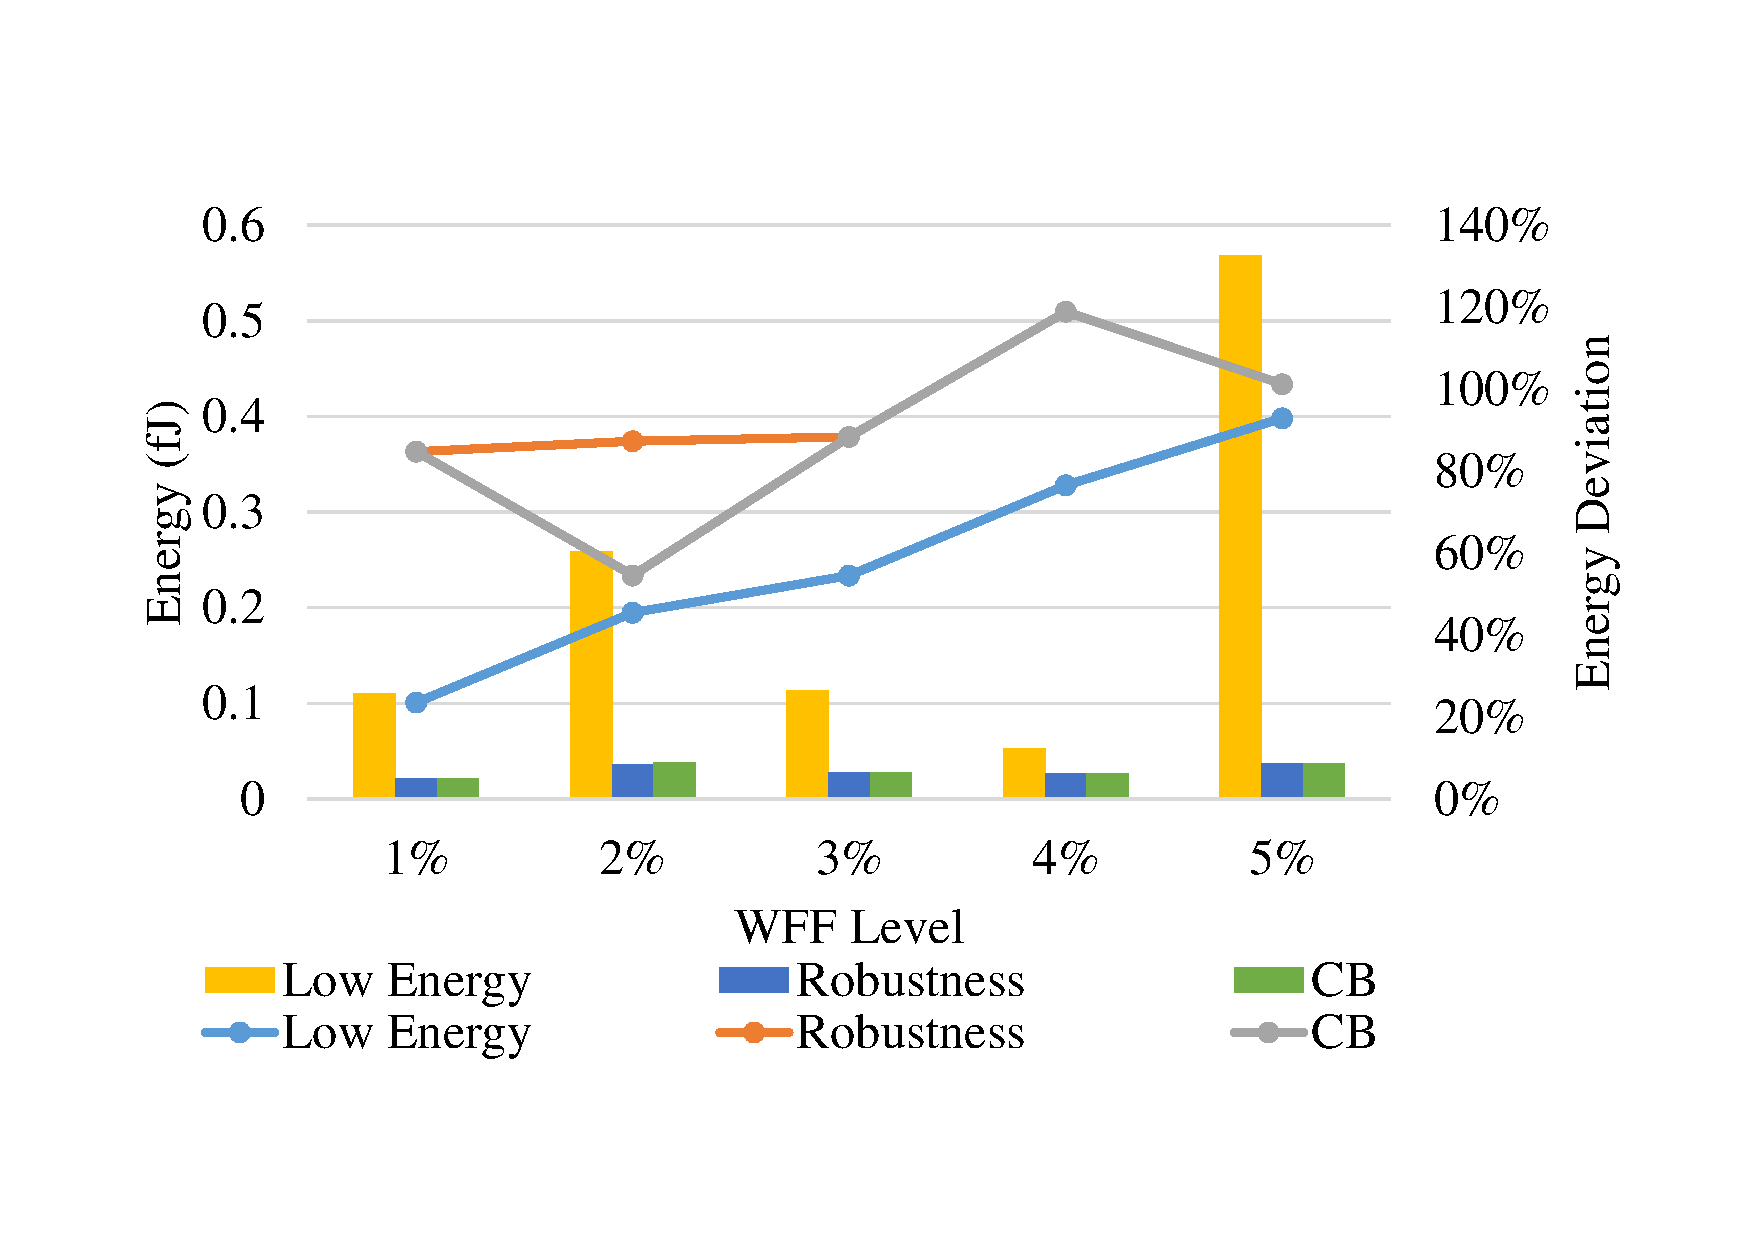
\includegraphics[width=1\textwidth, trim={1.25cm 2cm 2cm 3cm}, clip]{comp3Linv2Energy.pdf}
            \caption{Layout comparison for each scenario considering the energy metrics for the inverter.}
        \label{figscCompINV}
    \end{figure}

    \begin{figure}[]
        \centering
            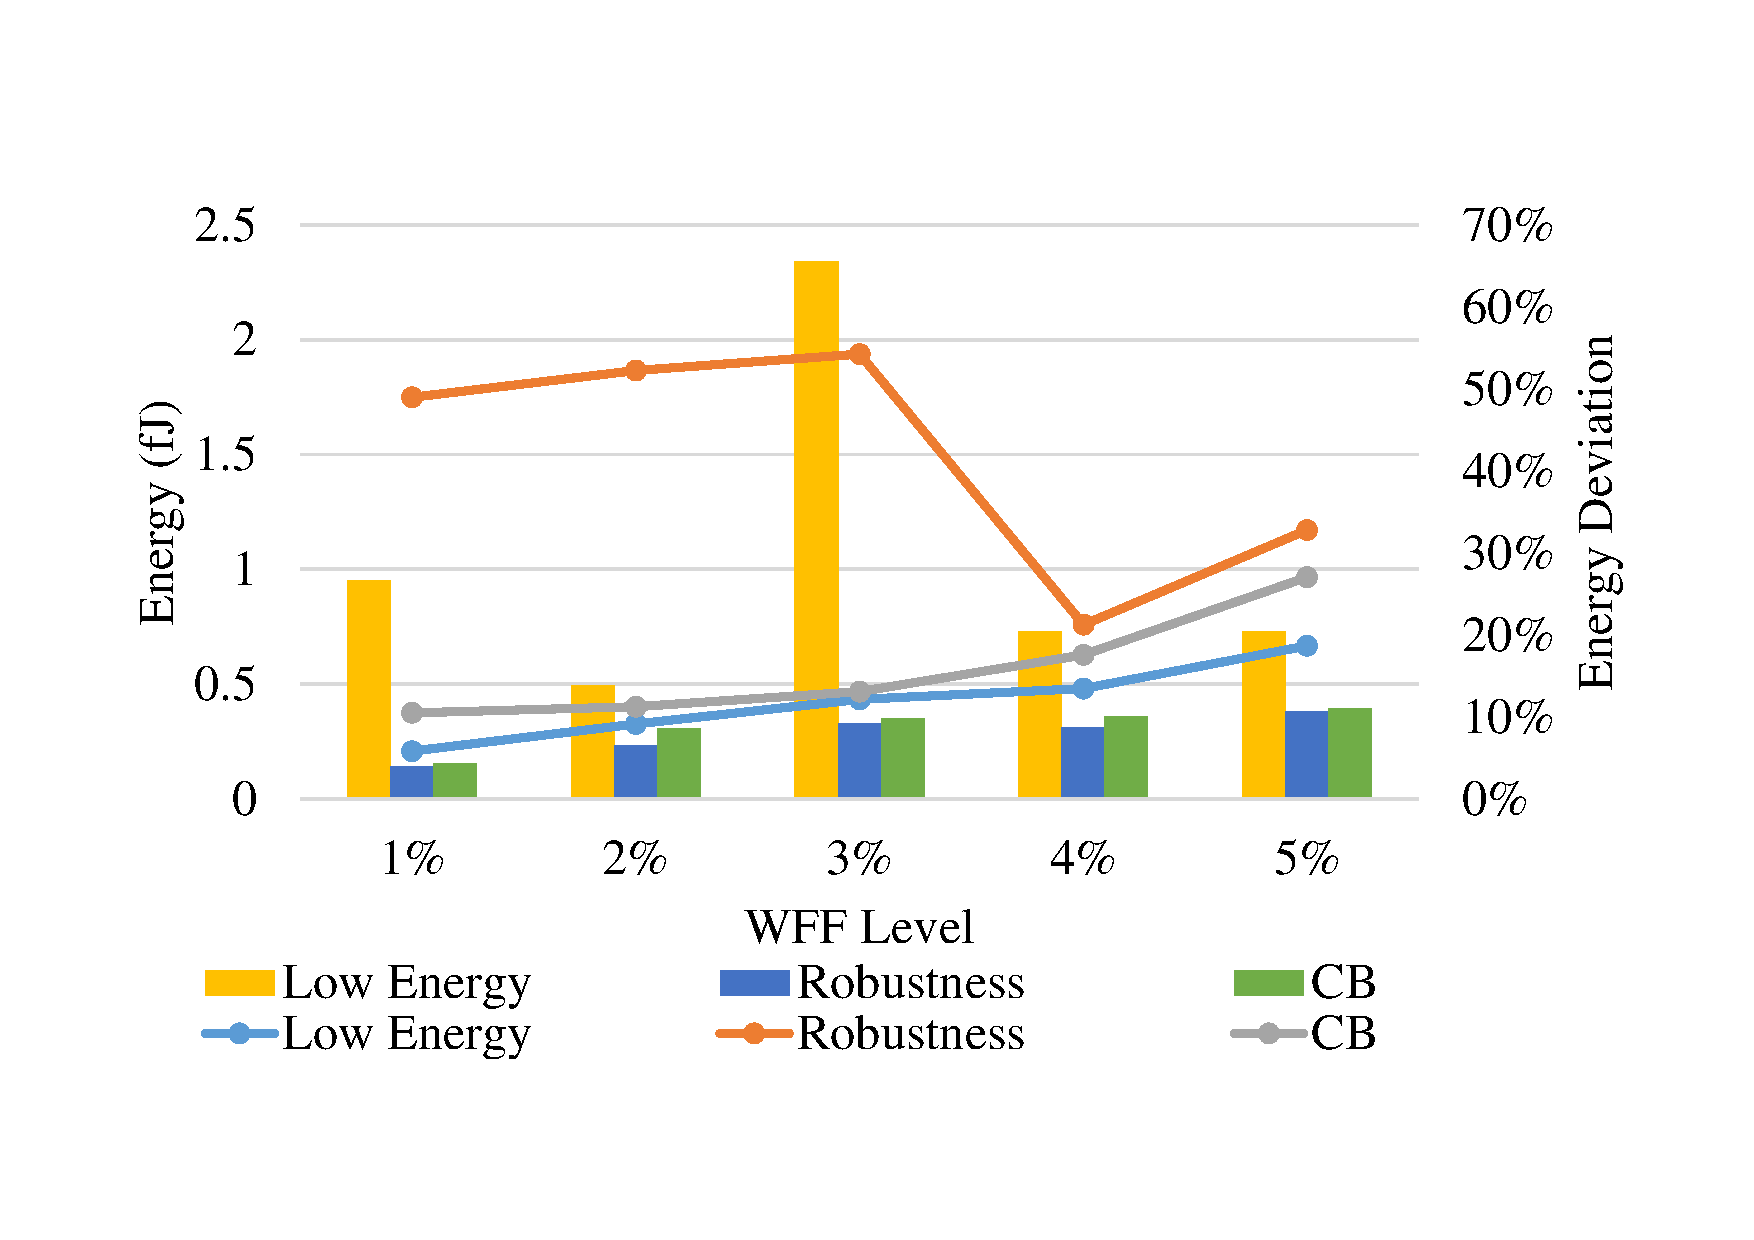
\includegraphics[width=1\textwidth, trim={1.25cm 3cm 2cm 3cm}, clip]{comp3Lst2Energy.pdf}
            \caption{Layout comparison for each scenario considering the energy metrics for the ST.}
        \label{figscCompST}
    \end{figure}

    \begin{figure}[]
        \centering
            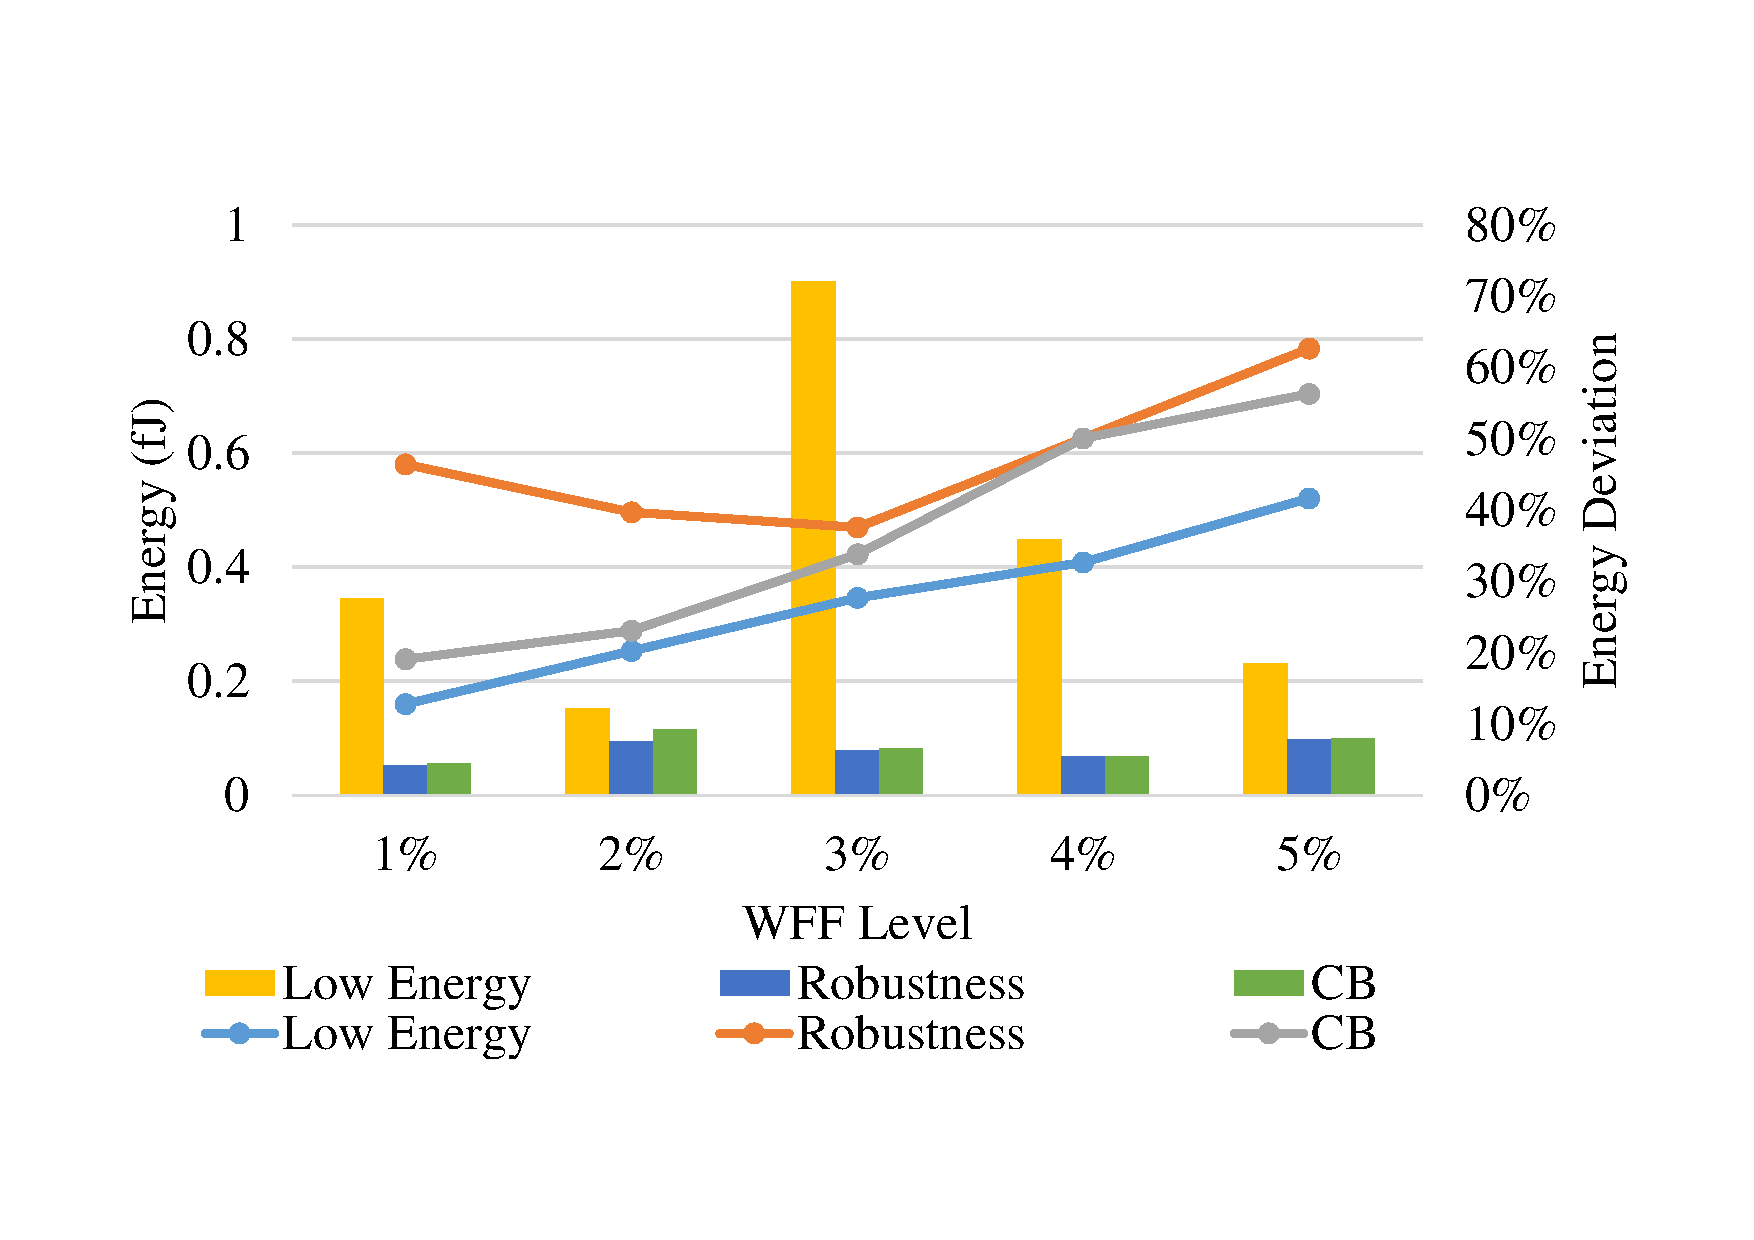
\includegraphics[width=1\textwidth, trim={1.25cm 3cm 2cm 3cm}, clip]{comp3Lsig2Energy.pdf}
            \caption{Layout comparison for each scenario considering the energy metrics for the SIG.}
        \label{figscCompSIG}
    \end{figure}

    \begin{figure}[]
        \centering
            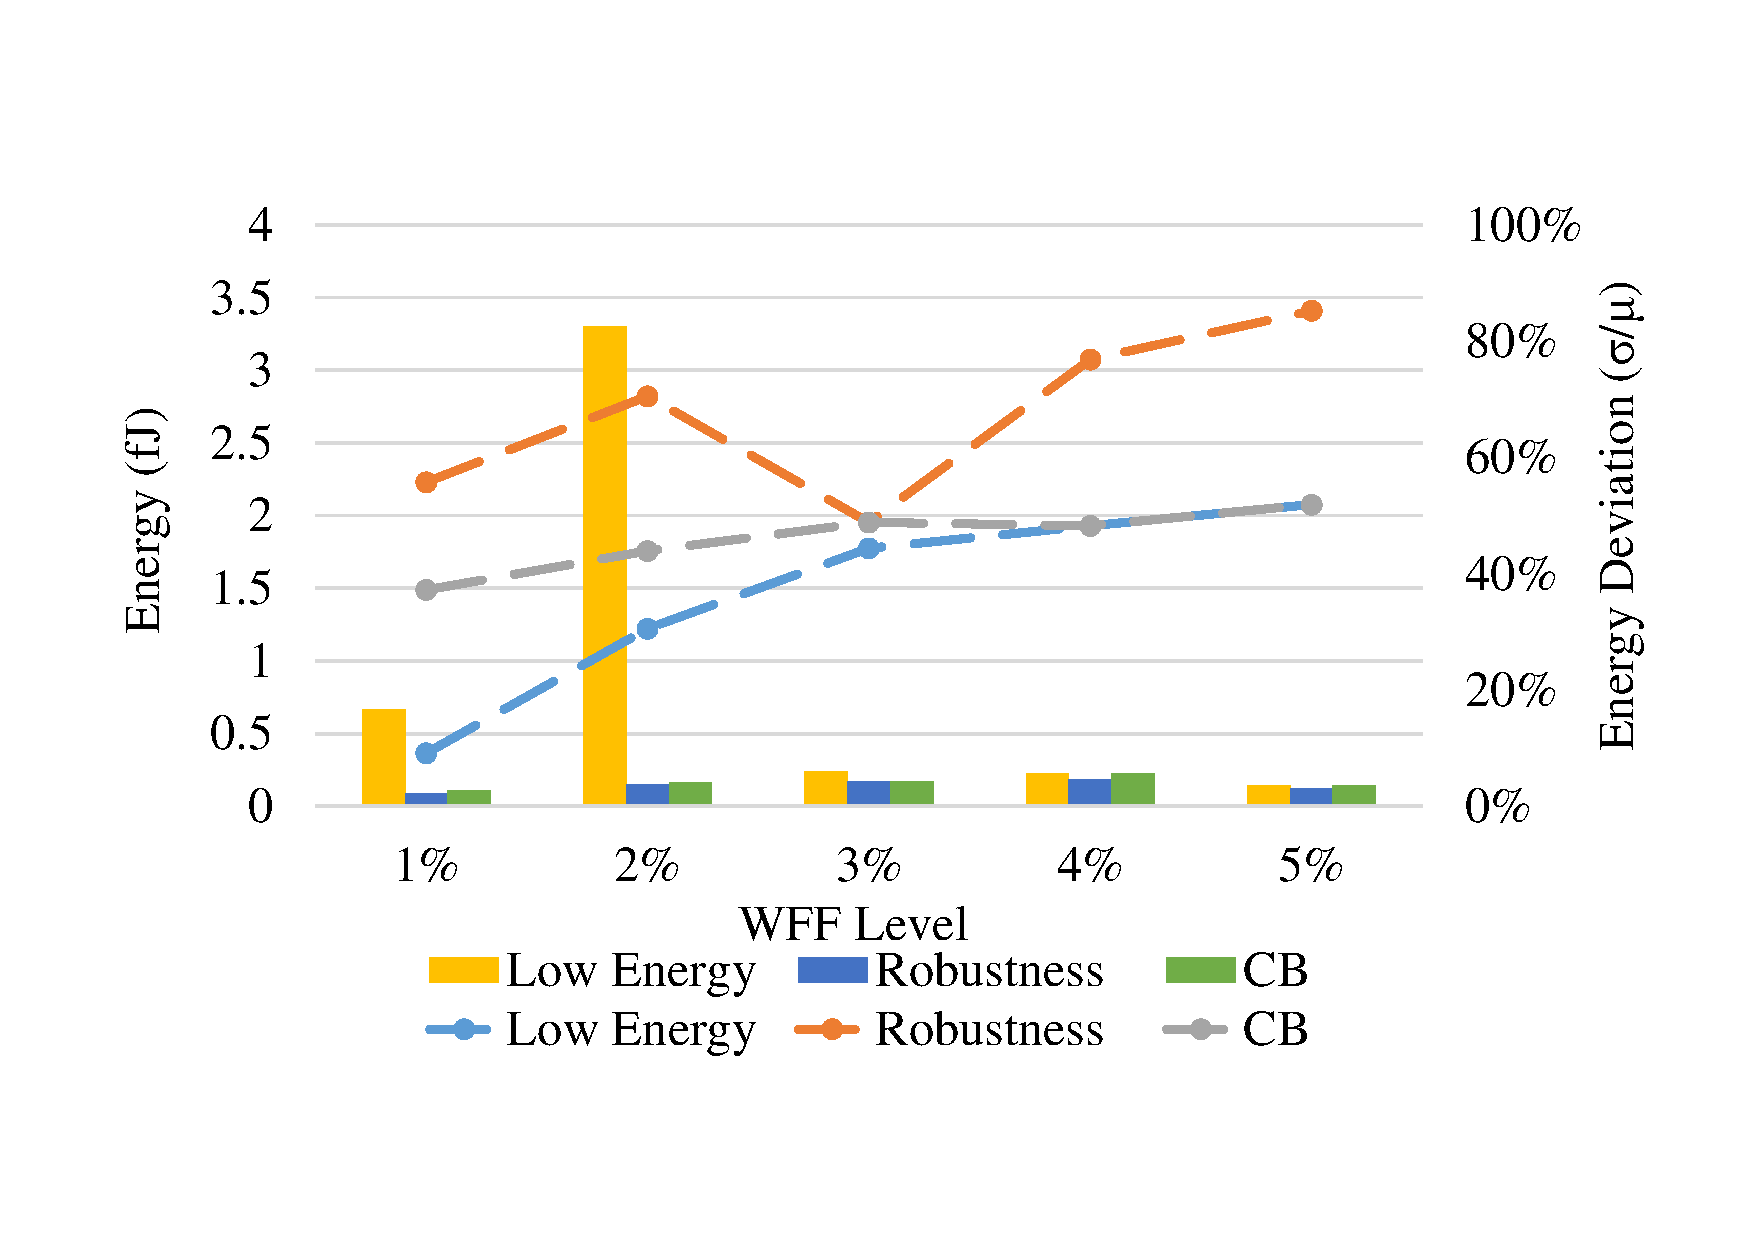
\includegraphics[width=1\textwidth, trim={1.25cm 3cm 2cm 3cm}, clip]{comp3Ltist212Energy.pdf}
            \caption{Layout comparison for each scenario considering the energy metrics for the TIST at 2:1 proportion.}
        \label{figscCompTIST21}
    \end{figure}

    \begin{figure}[]
        \centering
            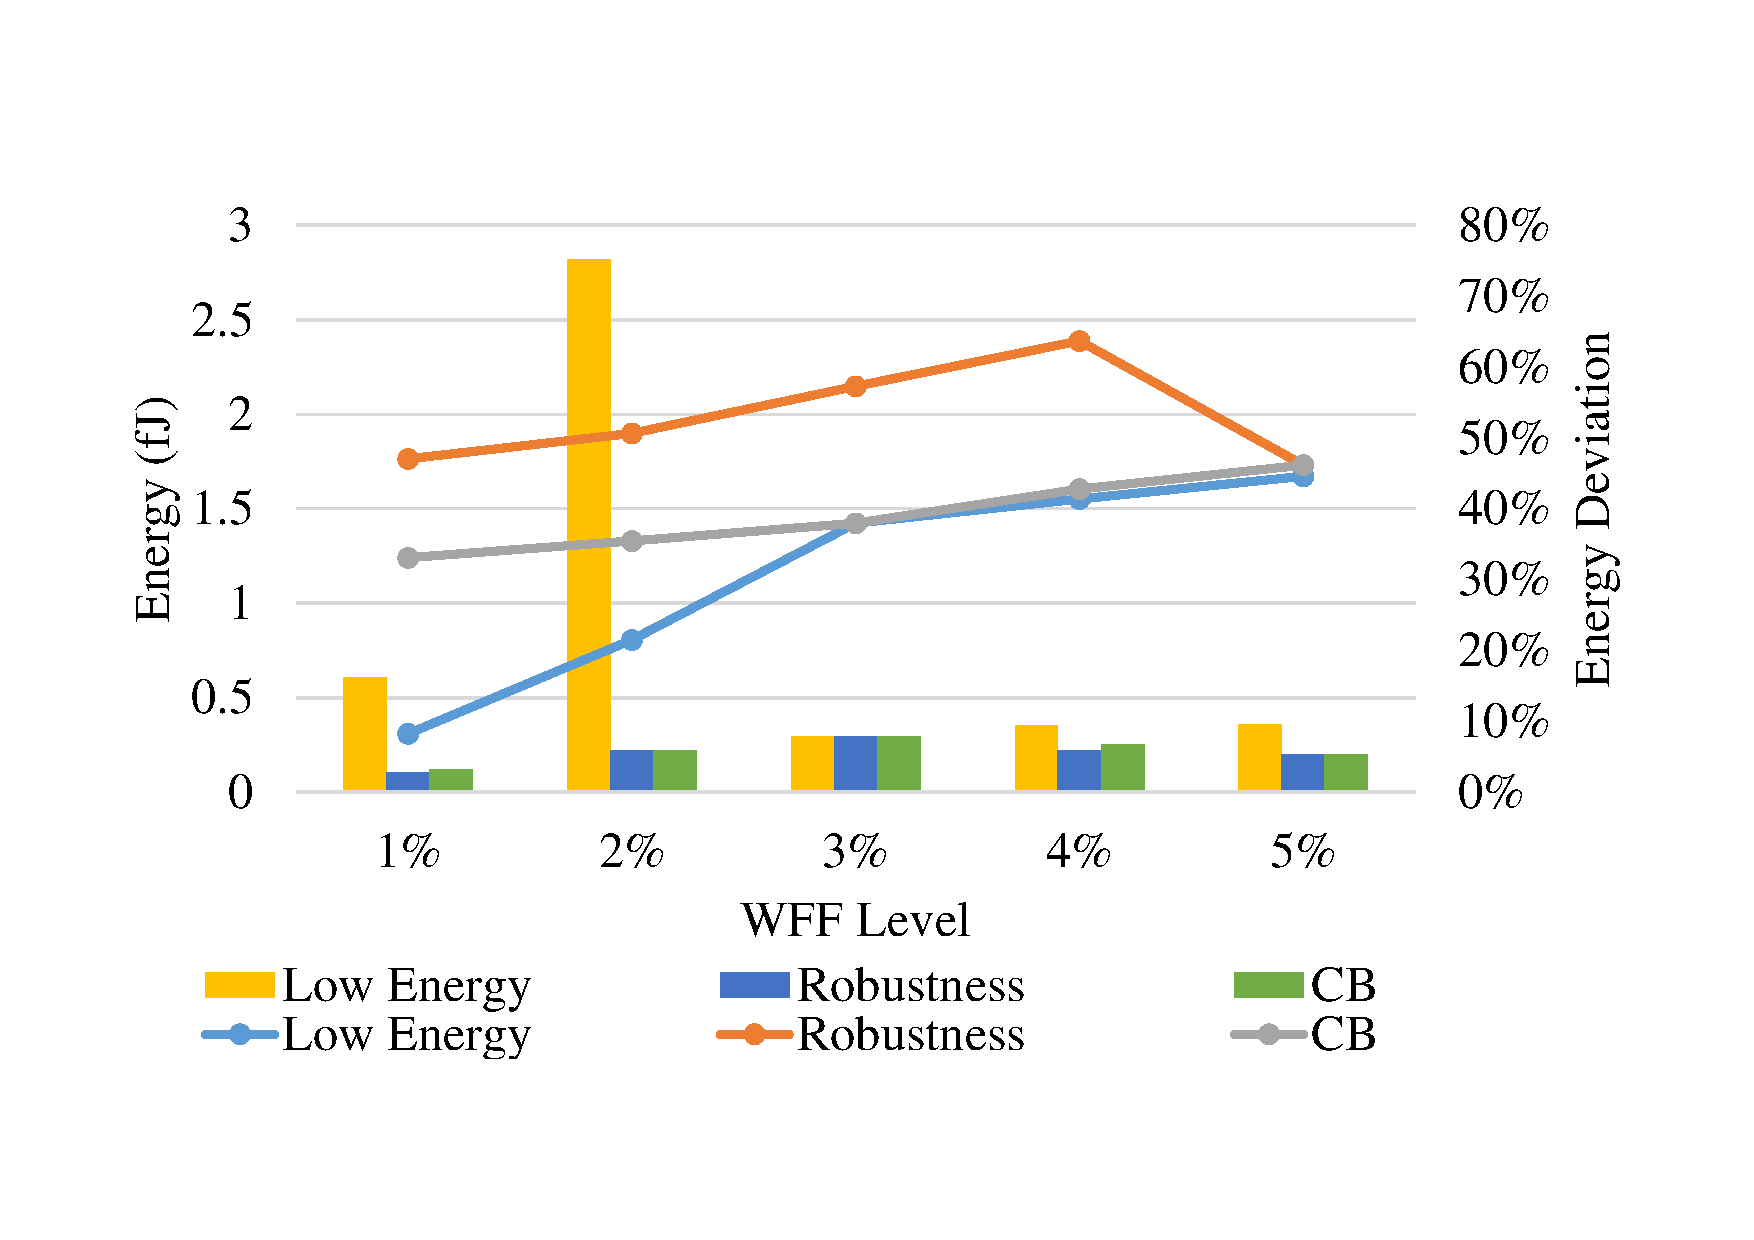
\includegraphics[width=1\textwidth, trim={1.25cm 3cm 2cm 3cm}, clip]{comp3Ltist312Energy.pdf}
            \caption{Layout comparison for each scenario considering the energy metrics for the TIST at 3:1 proportion.}
        \label{figscCompTIST31}
    \end{figure}

    A comparison between each design layout is presented in Fig. \ref{figCompLowEnergy}, Fig. \ref{figCompHighRobustness}, and Fig. \ref{figCompCB}. The lines correspond to the energy consumption axis (left), while the bars correspond to the energy deviation axis (right). Considering the averages, for the low energy layouts, the inverter presented the lowest energy consumption, followed by the SIG (34.61\% higher), ST (68.32\% higher), TIST 3:1 (358.84\% higher) and TIST 2:1 (487\% higher), respectively. The TIST layouts, showed the highest robustness, with the 2:1 variants presenting a 22.93\% average energy deviation and the 3:1 variants showing a minor increase with its 23.62\% average energy deviation. Following the TIST layouts, the ST, SIG and inverter present a 29.34\%, 33.25\%, and 51.55\% energy deviation, respectively. It can be noted that, while the inverter presents the lowest energy consumption it presents the highest energy deviation as well. It is mainly due to its spike on deviation at 5\% WFF but even disconsidering this spike, the inverter would show an average deviation of 31.25\%, which is still higher than most designs. Given so, the inverter is not entirely recommended for a low energy application where robustness is critical. A more appropriate design would be either ST or SIG, with the ST although presenting higher energy consumption, its hysteresis effect should not be ignored, being of importance for high noise application.

    \begin{figure}[]
        \centering
            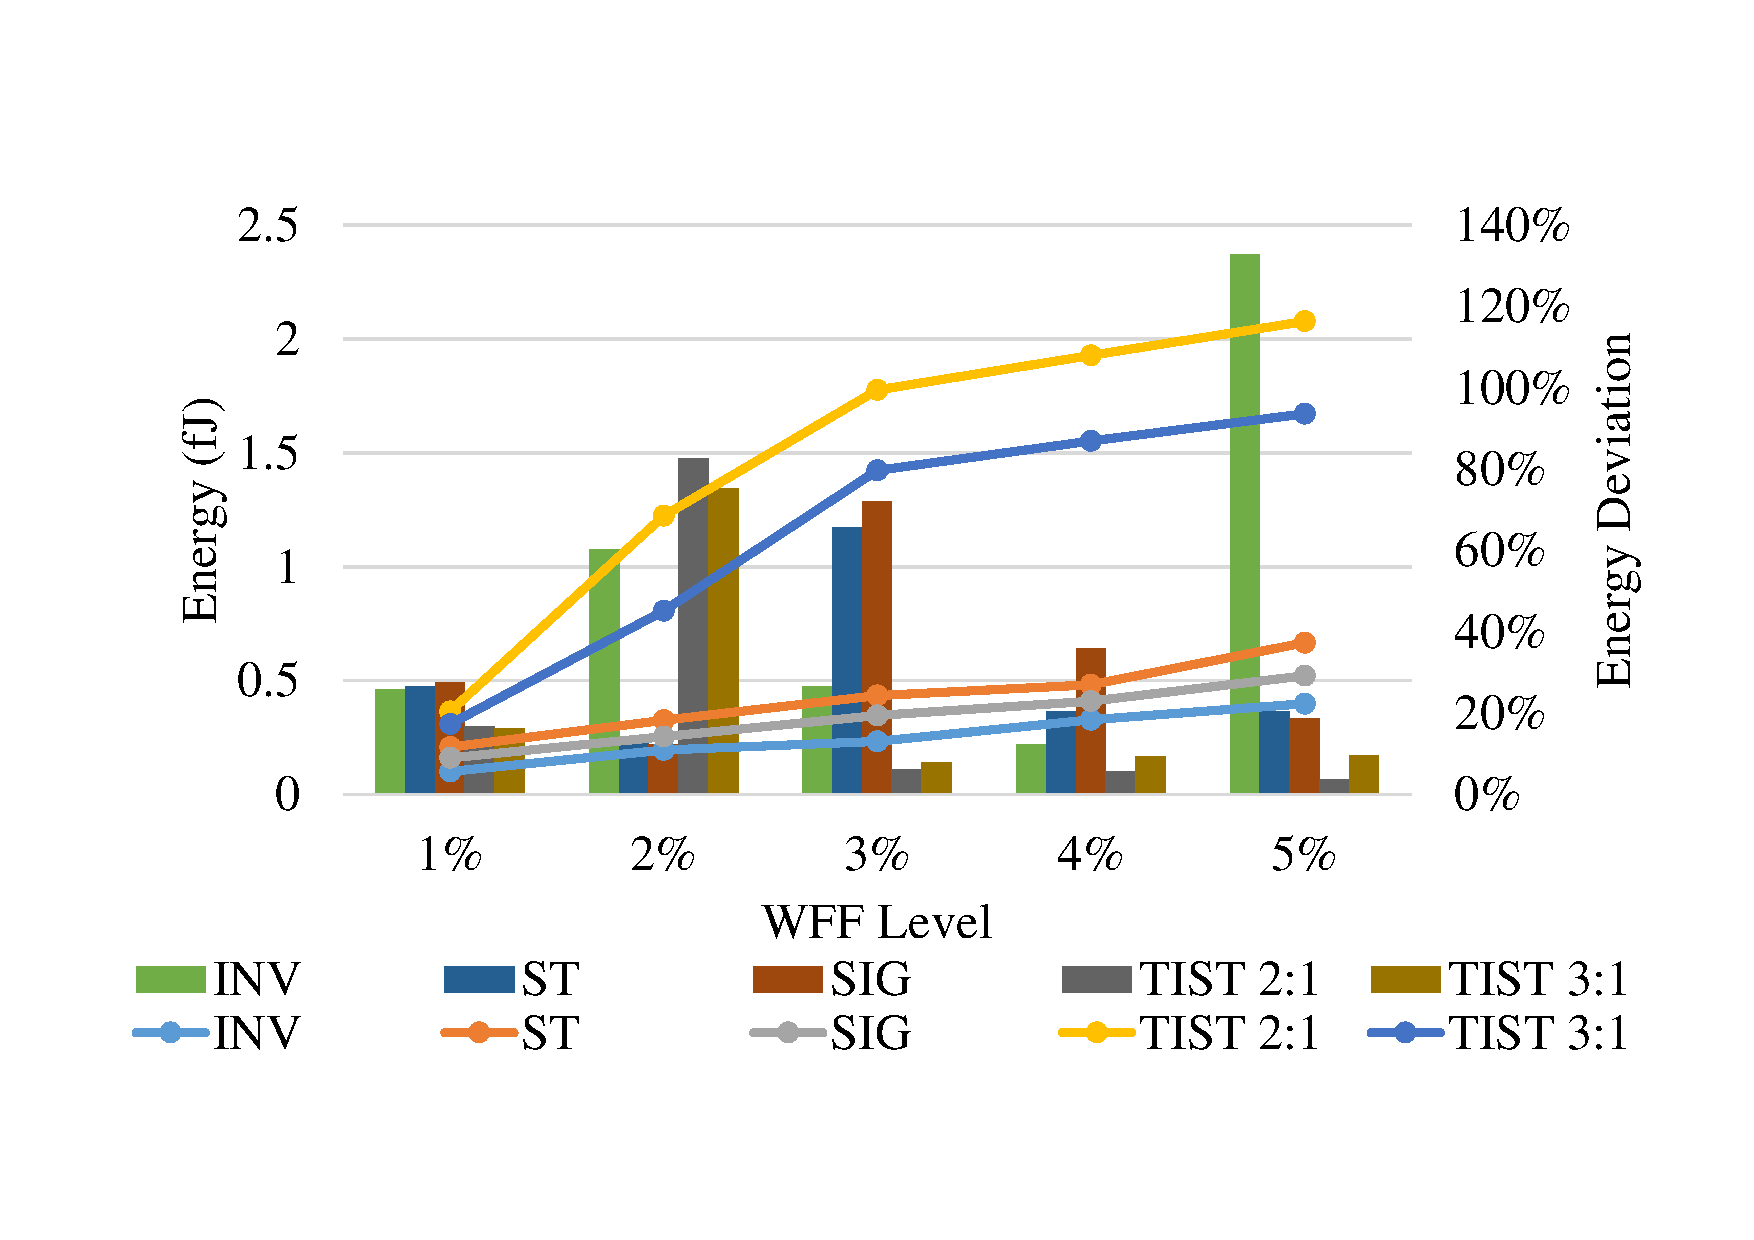
\includegraphics[width=1\textwidth, trim={1.25cm 3cm 2cm 3cm}, clip]{compLowEnergy.pdf}
            \caption{Low energy layouts energy metrics comparison for each design.}
        \label{figCompLowEnergy}
    \end{figure}

    For the high robustness spectrum, the energy consumption difference between designs follows the same behaviour, although with much broader differences. In comparison to the inverter energy consumption each design presented an average increase of 43.52\%, 263.24\%, 382.12\%, and 555.21\%, for the SIG, ST, TIST 3:1, and TIST 2:1, respectively. The deviation metrics presented a similar behaviour as well, although the ST presented the highest deviations. The TIST designs presented the lowest deviations with 3.56\%, and 5.55\% for the TIST 2:1, and 3:1, respectively. Following, the SIG, inverter, and ST, presented 6.23\%, 6.93\%, and 7.81\% deviations. In this case, the inverter is a strong candidate, with the lowest energy consumption, and acceptable robustness.

    \begin{figure}[]
        \centering
            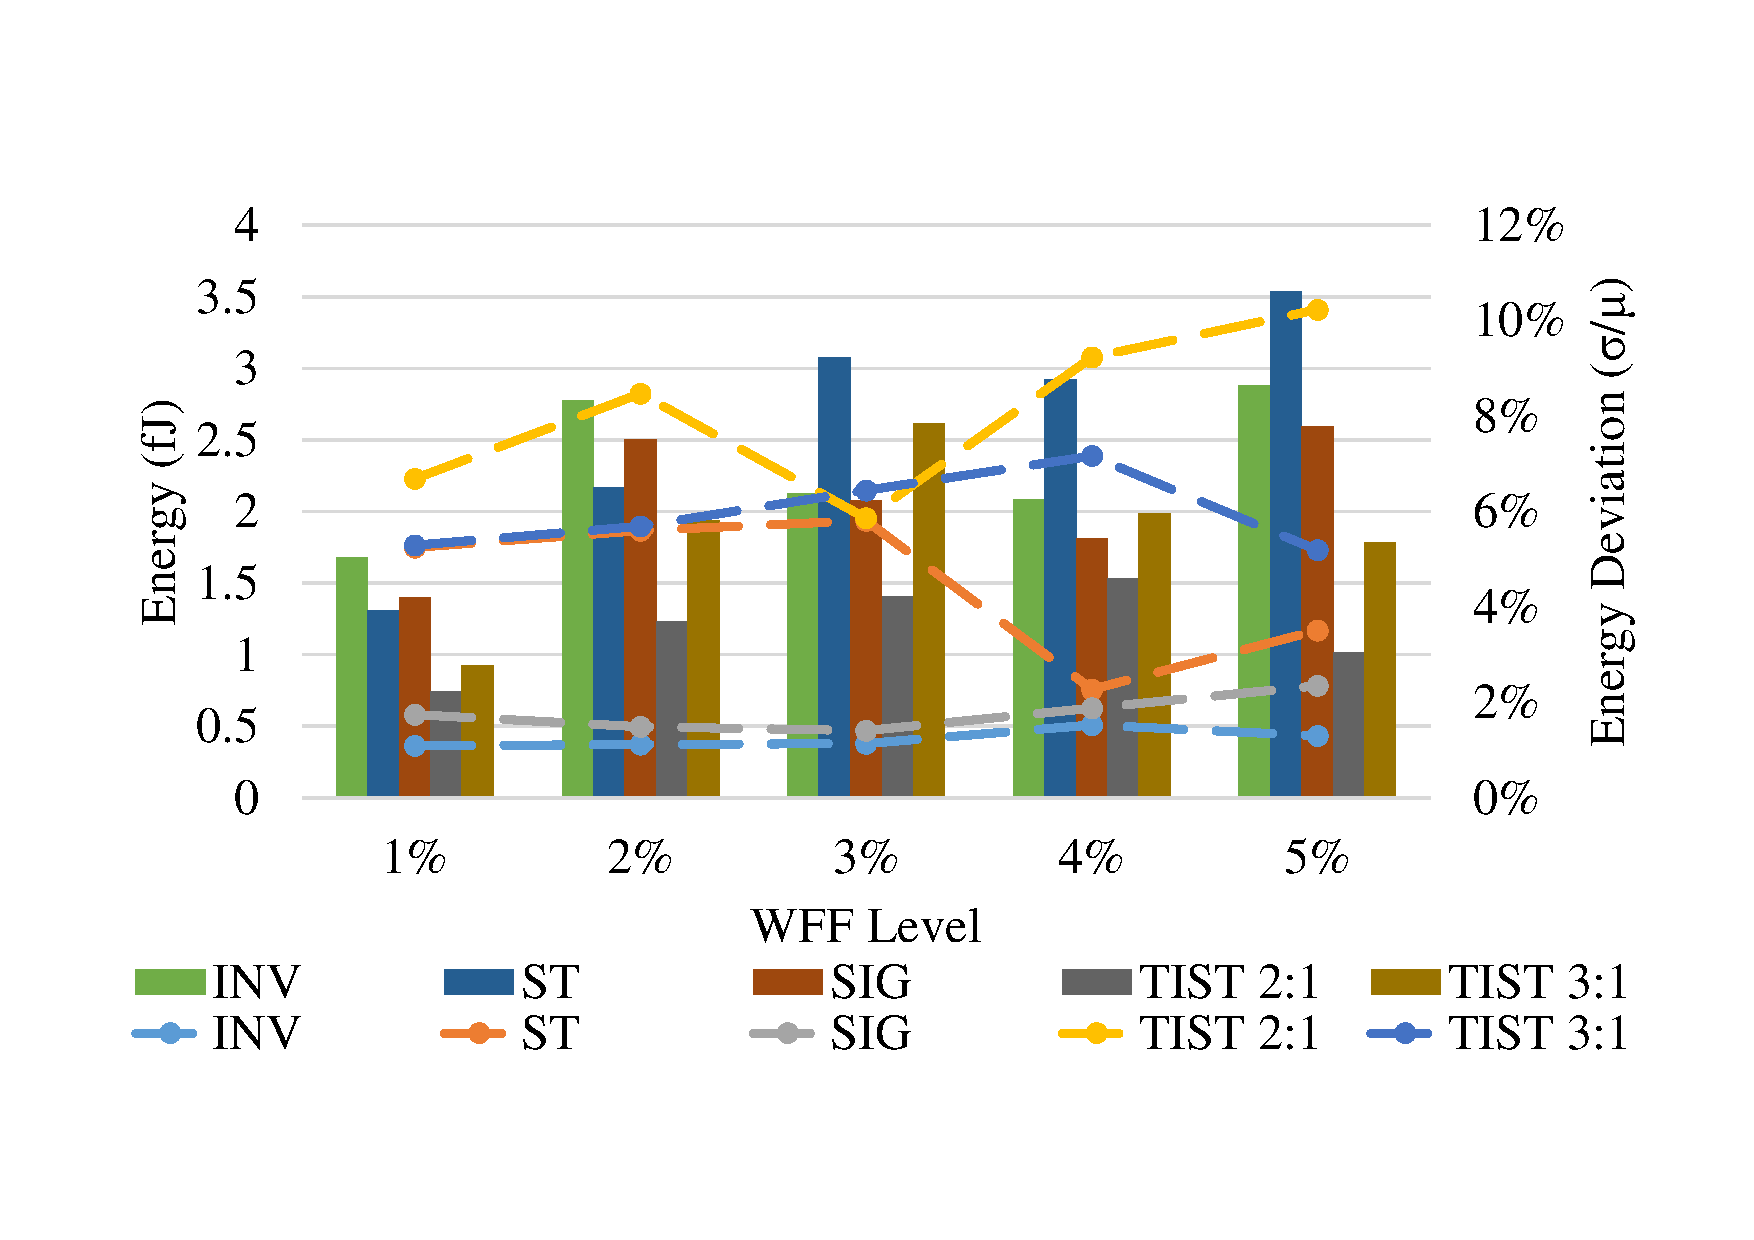
\includegraphics[width=1\textwidth, trim={1.25cm 3cm 2cm 3cm}, clip]{compHighRobustness.pdf}
            \caption{High robustness layouts energy metrics comparison for each design.}
        \label{figCompHighRobustness}
    \end{figure}

    Lastly, for the CB layouts, the energy consumption scaling through the designs is the same, although with smaller differences, even in comparison to the low energy layouts. In comparison to the inverter, the SIG, ST, TIST 3:1, and TIST 2:1 presented average increases of 18.84\%, 47.74\%, 281.85\%, and 379.6\%. The designs kept the same behaviour as their high robustness variants. The TIST designs presented the lowest deviations with 4.07\% and 5.8\% for the 2:1 and 3:1 proportions, respectively. The SIG, inverter and ST, presented respectively, 6.72\%, 7.05\%, and 8.74\% deviations on energy. In this case, the SIG, presents a higher energy consumption and much bigger layout, it only provides a minor improvement over deviations (4.91\%, relative to the inverter). The ST presented higher energy and bigger area as well, with a increase on deviations (1.69\%, absolute and 23.97\% relative increases, in comparison to the inverter), although it still presents hysteresis. The TIST designs, consume considerably more energy, with less deviation (although, as stated before, those numbers are deflated), bigger layout area, and less viable scenarios to work with.

    \begin{figure}[]
        \centering
            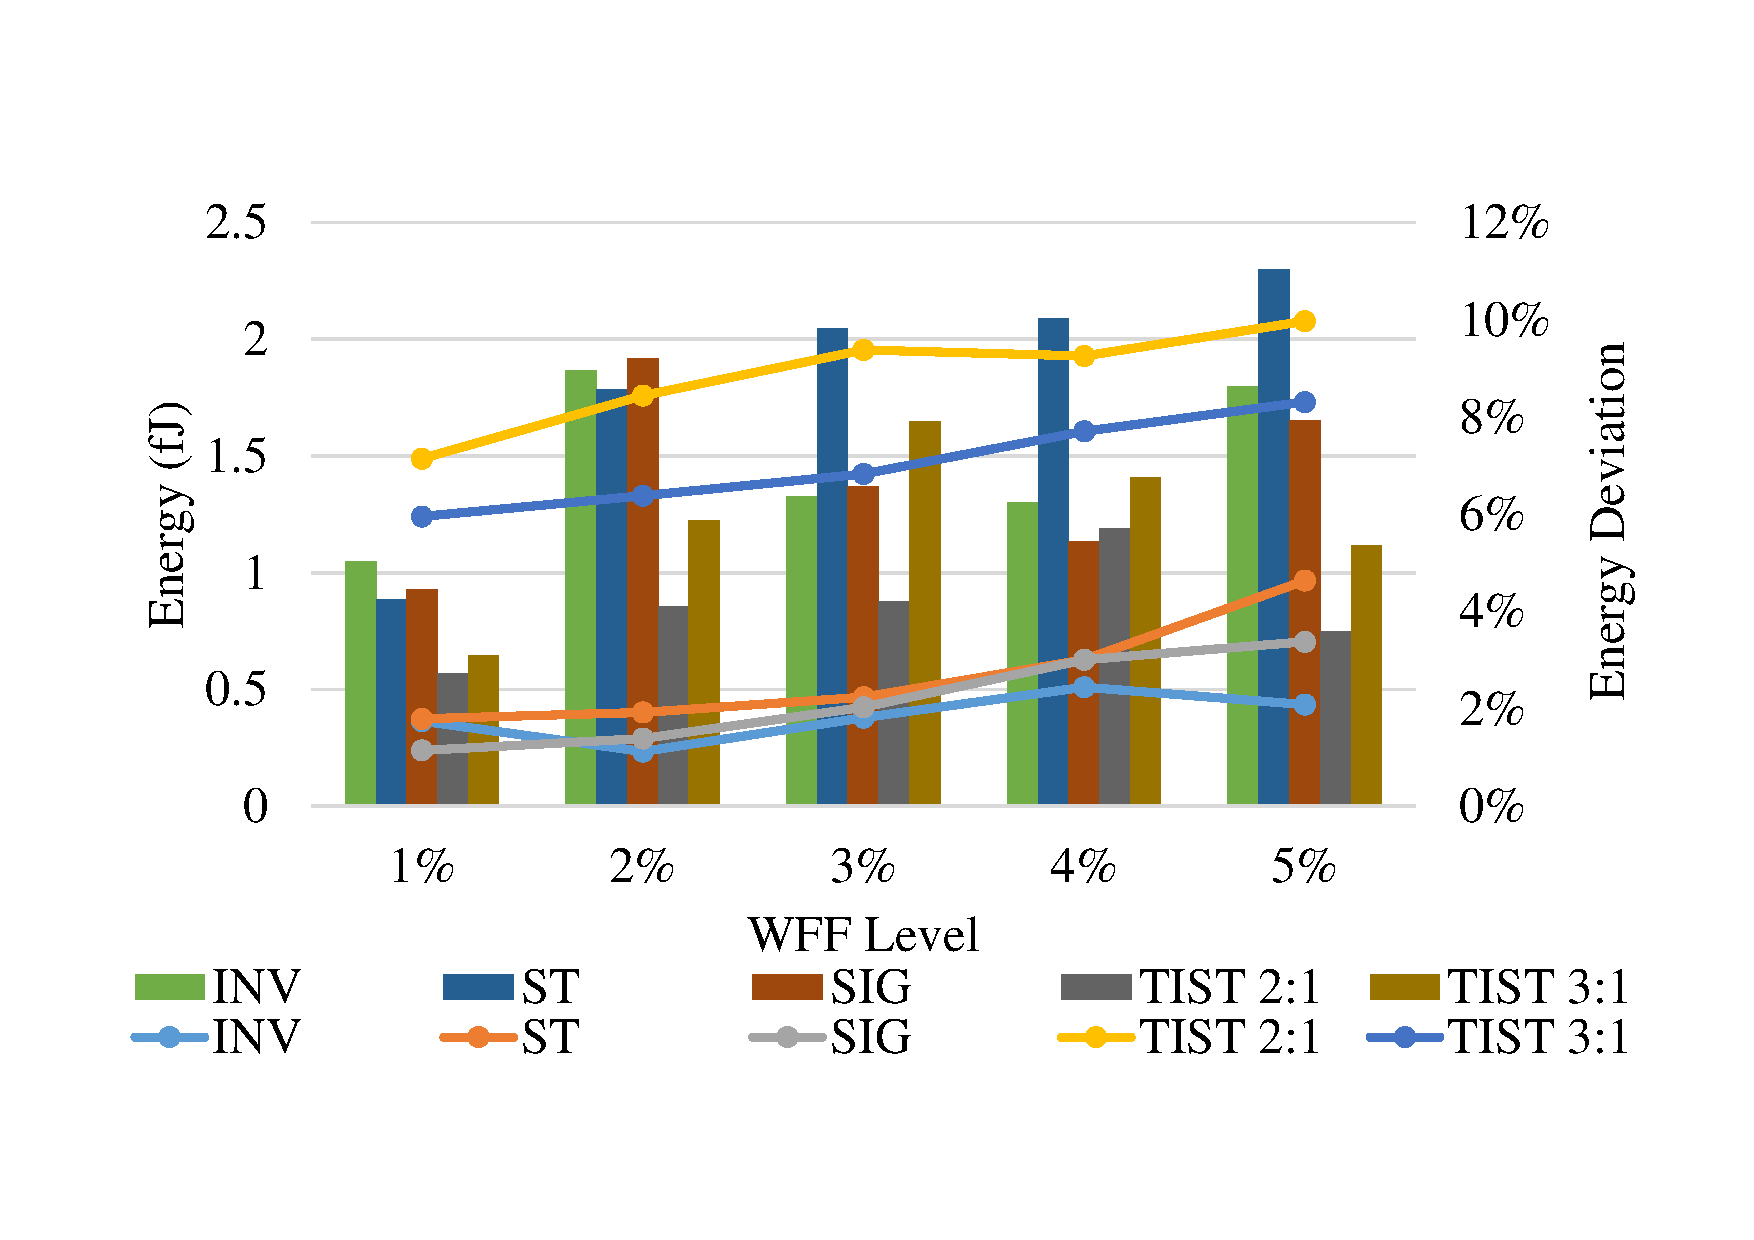
\includegraphics[width=1\textwidth, trim={1.25cm 3cm 2cm 3cm}, clip]{compCB.pdf}
            \caption{CB layouts energy metrics comparison for each design.}
        \label{figCompCB}
    \end{figure}


\section{Static Noise Margins}

    The evaluation of the Static Noise Margins (SNM) are shown at Table \ref{tab:SNM}. The inverter and SIG showed identical SNMs, while TIST designs presented higher SNMs than the inverter and SIG at sub-threshold levels, with the 2:1 layouts presenting lower margins. The ST presented higher SNMs overall. In comparison to the inverter, SIG, and TIST 3:1, which presented the same average SNM of 0.164V, the TIST 2:1 presented 2.6\% lower SNMs, while the ST showed 17.5\% higher SNMs. The ST presents its biggest difference at low supply voltages, with 41.91\% and 28.23\% higher SNMs at 0.1V, and 0.2V, respectively, in comparison to the inverter.

\begin{table}[]
\centering
\caption{}
\label{tab:SNM}
\resizebox{\textwidth}{!}{%
\begin{tabular}{|c|c|c|c|c|c|c|c|c|}
\hline
\multirow{2}{*}{Design} &
  \multirow{2}{*}{SNM (V)} &
  \multicolumn{7}{c|}{Supply Voltage (V)} \\ \cline{3-9}
 &
   &
  0.1 &
  0.2 &
  0.3 &
  0.4 &
  0.5 &
  0.6 &
  0.7 \\ \hline
\multirow{3}{*}{INV} &
  $NM_{L}$ &
  0.025 &
  0.074 &
  0.122 &
  0.171 &
  0.217 &
  0.253 &
  0.277 \\ \cline{2-9}
 &
  $NM_{H}$ &
  0.025 &
  0.073 &
  0.121 &
  0.169 &
  0.216 &
  0.259 &
  0.299 \\ \cline{2-9}
 &
  \textbf{Avg.} &
  \textbf{0.025} &
  \textbf{0.073} &
  \textbf{0.122} &
  \textbf{0.170} &
  \textbf{0.216} &
  \textbf{0.256} &
  \textbf{0.288} \\ \hline
\multirow{3}{*}{SIG} &
  $NM_{L}$ &
  0.025 &
  0.074 &
  0.122 &
  0.171 &
  0.217 &
  0.253 &
  0.277 \\ \cline{2-9}
 &
  $NM_{H}$ &
  0.025 &
  0.073 &
  0.121 &
  0.169 &
  0.216 &
  0.259 &
  0.299 \\ \cline{2-9}
 &
  \textbf{Avg.} &
  \textbf{0.025} &
  \textbf{0.073} &
  \textbf{0.122} &
  \textbf{0.170} &
  \textbf{0.216} &
  \textbf{0.256} &
  \textbf{0.288} \\ \hline
\multirow{3}{*}{ST} &
  $NM_{L}$ &
  0.036 &
  0.111 &
  0.178 &
  0.244 &
  0.310 &
  0.376 &
  0.440 \\ \cline{2-9}
 &
  $NM_{H}$ &
  0.036 &
  0.077 &
  0.111 &
  0.144 &
  0.178 &
  0.213 &
  0.248 \\ \cline{2-9}
 &
  \textbf{Avg.} &
  \textbf{0.036} &
  \textbf{0.094} &
  \textbf{0.144} &
  \textbf{0.194} &
  \textbf{0.244} &
  \textbf{0.294} &
  \textbf{0.344} \\ \hline
\multirow{3}{*}{TIST 2:1} &
  $NM_{L}$ &
  0.061 &
  0.161 &
  0.245 &
  0.292 &
  0.319 &
  0.337 &
  0.359 \\ \cline{2-9}
 &
  $NM_{H}$ &
  0.014 &
  0.007 &
  0.010 &
  0.038 &
  0.079 &
  0.131 &
  0.189 \\ \cline{2-9}
 &
  \textbf{Avg.} &
  \textbf{0.037} &
  \textbf{0.084} &
  \textbf{0.128} &
  \textbf{0.165} &
  \textbf{0.199} &
  \textbf{0.234} &
  \textbf{0.274} \\ \hline
\multirow{3}{*}{TIST 3:1} &
  $NM_{L}$ &
  0.051 &
  0.150 &
  0.233 &
  0.277 &
  0.300 &
  0.314 &
  0.341 \\ \cline{2-9}
 &
  $NM_{H}$ &
  0.022 &
  0.017 &
  0.022 &
  0.056 &
  0.108 &
  0.173 &
  0.235 \\ \cline{2-9}
 &
  \textbf{Avg.} &
  \textbf{0.036} &
  \textbf{0.084} &
  \textbf{0.128} &
  \textbf{0.167} &
  \textbf{0.204} &
  \textbf{0.244} &
  \textbf{0.288} \\ \hline
\end{tabular}%
}
\end{table}

     Concerning the $I_{on}$/$I_{off}$ ratios, in comparison to the inverter, the ST, TIST 2:1, and TIST 3:1 presented, on average, 118.01\%, 600.21\%, and 468.7\% higher ratios. The SIG is the only design which presented a worsening with a 12.53\% lower ratio. While considering deviations into the ratio due to process variability, the ST and SIG presented 11.1\% and 6.91\% lower deviations, with the TIST 2:1 and 3:1 presenting 49.57\% and 42.79\% higher deviations, respectively. The current ratios and current ratios deviations are shown in Fig. \ref{figsCurrComp}, with the marked lines and bars being related to the left and right axis, respectively.

    \begin{figure}[]
        \centering
            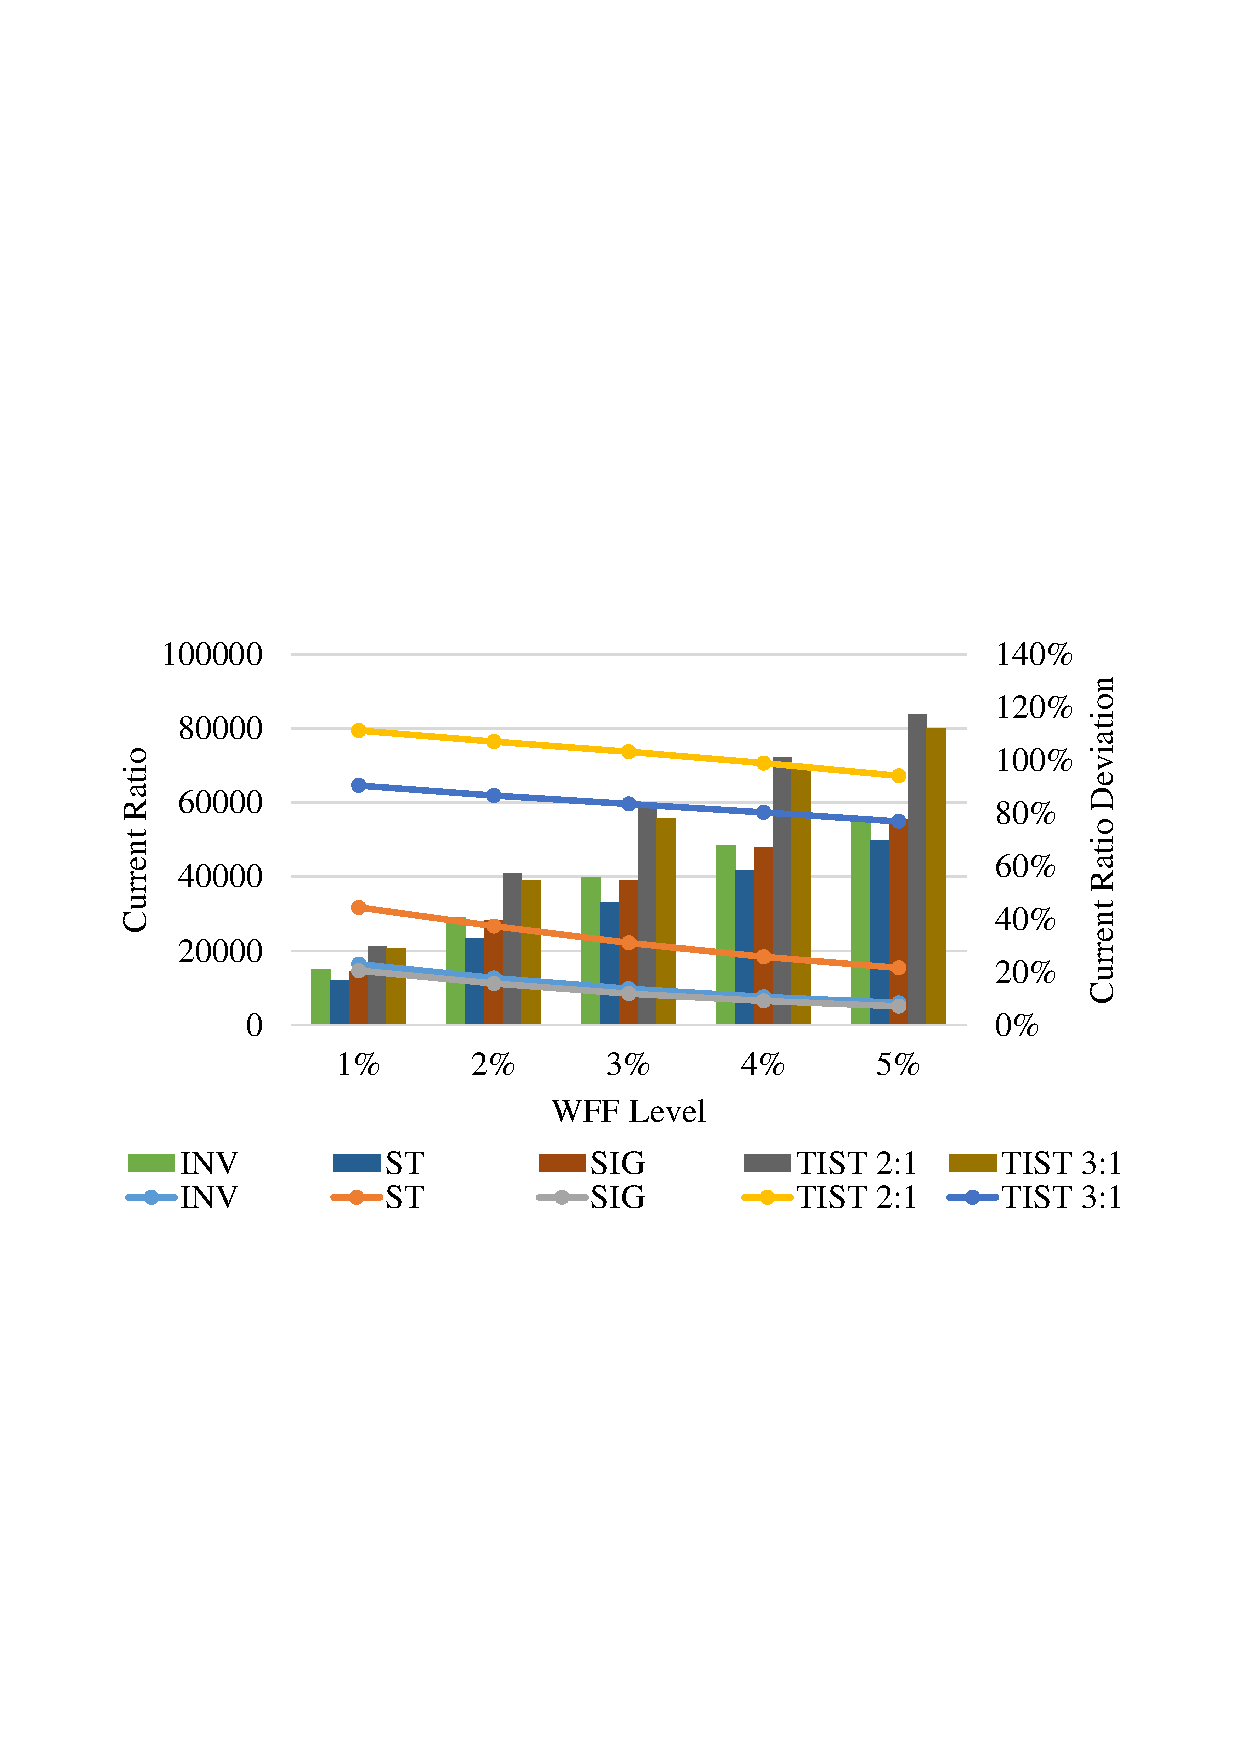
\includegraphics[width=1\textwidth, trim={1.25cm 9cm 2cm 10cm}, clip]{currRatioWFF.pdf}
            \caption{Current ratio (left) and current ratio deviation (right) design comparison across variability scaling.}
        \label{figsCurrComp}
    \end{figure}

    Due to the variability impact, the current ratios tend to decrease. This mainly happens due to the increase of the off-current as variability scales. This behavior is due to the effects of DIBL (Drain-Induced Barrier Lowering) and is a consequence of the short channel present on modern transistors. Due to the decreasing channel length, the depletion regions of drain and source become an increasing fraction of the whole area under the gate. Therefore, the volume of the depletion region effectively controlled by the gate decreases which can be modeled by a threshold voltage decreasing with the gate length. The charge below the gate being not only controlled by the gate but also by the drain and source regions is called the charge sharing effect. A similar effect occurs if the drain potential of the transistor increases: the pn-junction between the drain and the substrate becomes more reverse-biased, so the depletion layer grows and reduces even more the volume controlled by the gate. Given so, a drain bias-dependent threshold voltage can be assumed, as shown in Equation \ref{eqn:DIBL} \cite{henzler2006power}:

      \begin{equation}
        \centering
        \label{eqn:DIBL}
        V_{th} = V_{th,0} - mV_{DS}
    \end{equation}

    Thus, according to Equation \ref{eqn:sub} \cite{henzler2006power}, where $I_{D,sub}$ is the subthreshold current (leakage current), the leakage current (or subthreshold current) is exponentially dependent on the threshold voltage, as shown in Fig. \ref{figsOffCurrComp} for the inverter, although all designs presented the same behavior. The TIST designs presented the lowest decrease, at 15.21\%, with the ST, inverter, and SIG presenting much higher losses with 51.44\%, 63.59\%, 65.54\%, respectively. The current ratios present a linear decrease, instead of an exponential decrease, due to the lower, although exponential, increase rate of the $on$ current, as shown in Fig. \ref{figOnOffScal}.

    \begin{equation}
        \centering
        \label{eqn:sub}
        I_{D,sub} = I_0 \cdot exp\left(\frac{V_{GS} - V_{th,0} + mV_{DS}}{\eta \cdot V_T}\right)
    \end{equation}

    \begin{figure}[]
        \centering
            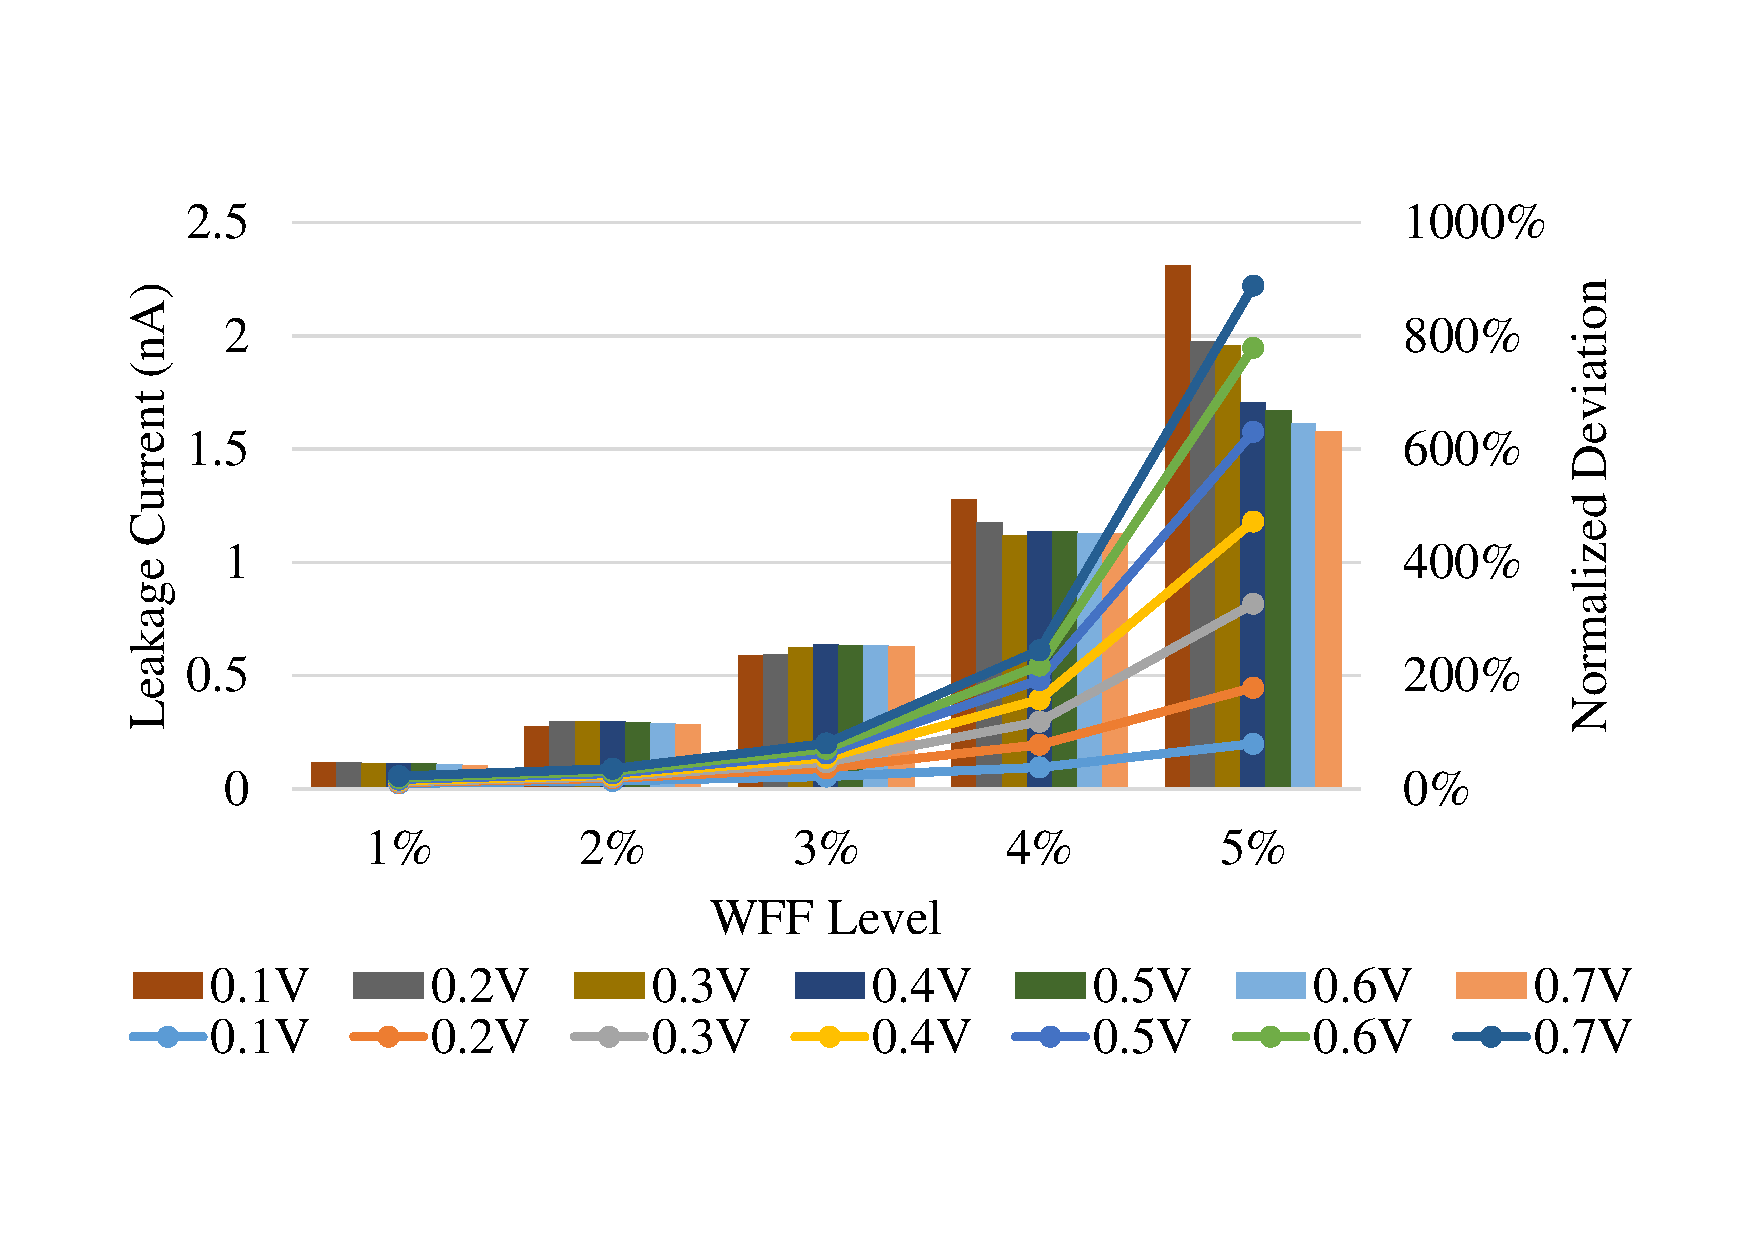
\includegraphics[width=1\textwidth, trim={1.25cm 3cm 2cm 3cm}, clip]{offCurrentComp.pdf}
            \caption{Leakage current scaling (left axis) and standard deviation (right axis) for the inverter.}
        \label{figsOffCurrComp}
    \end{figure}

    \begin{figure}[]
        \centering
            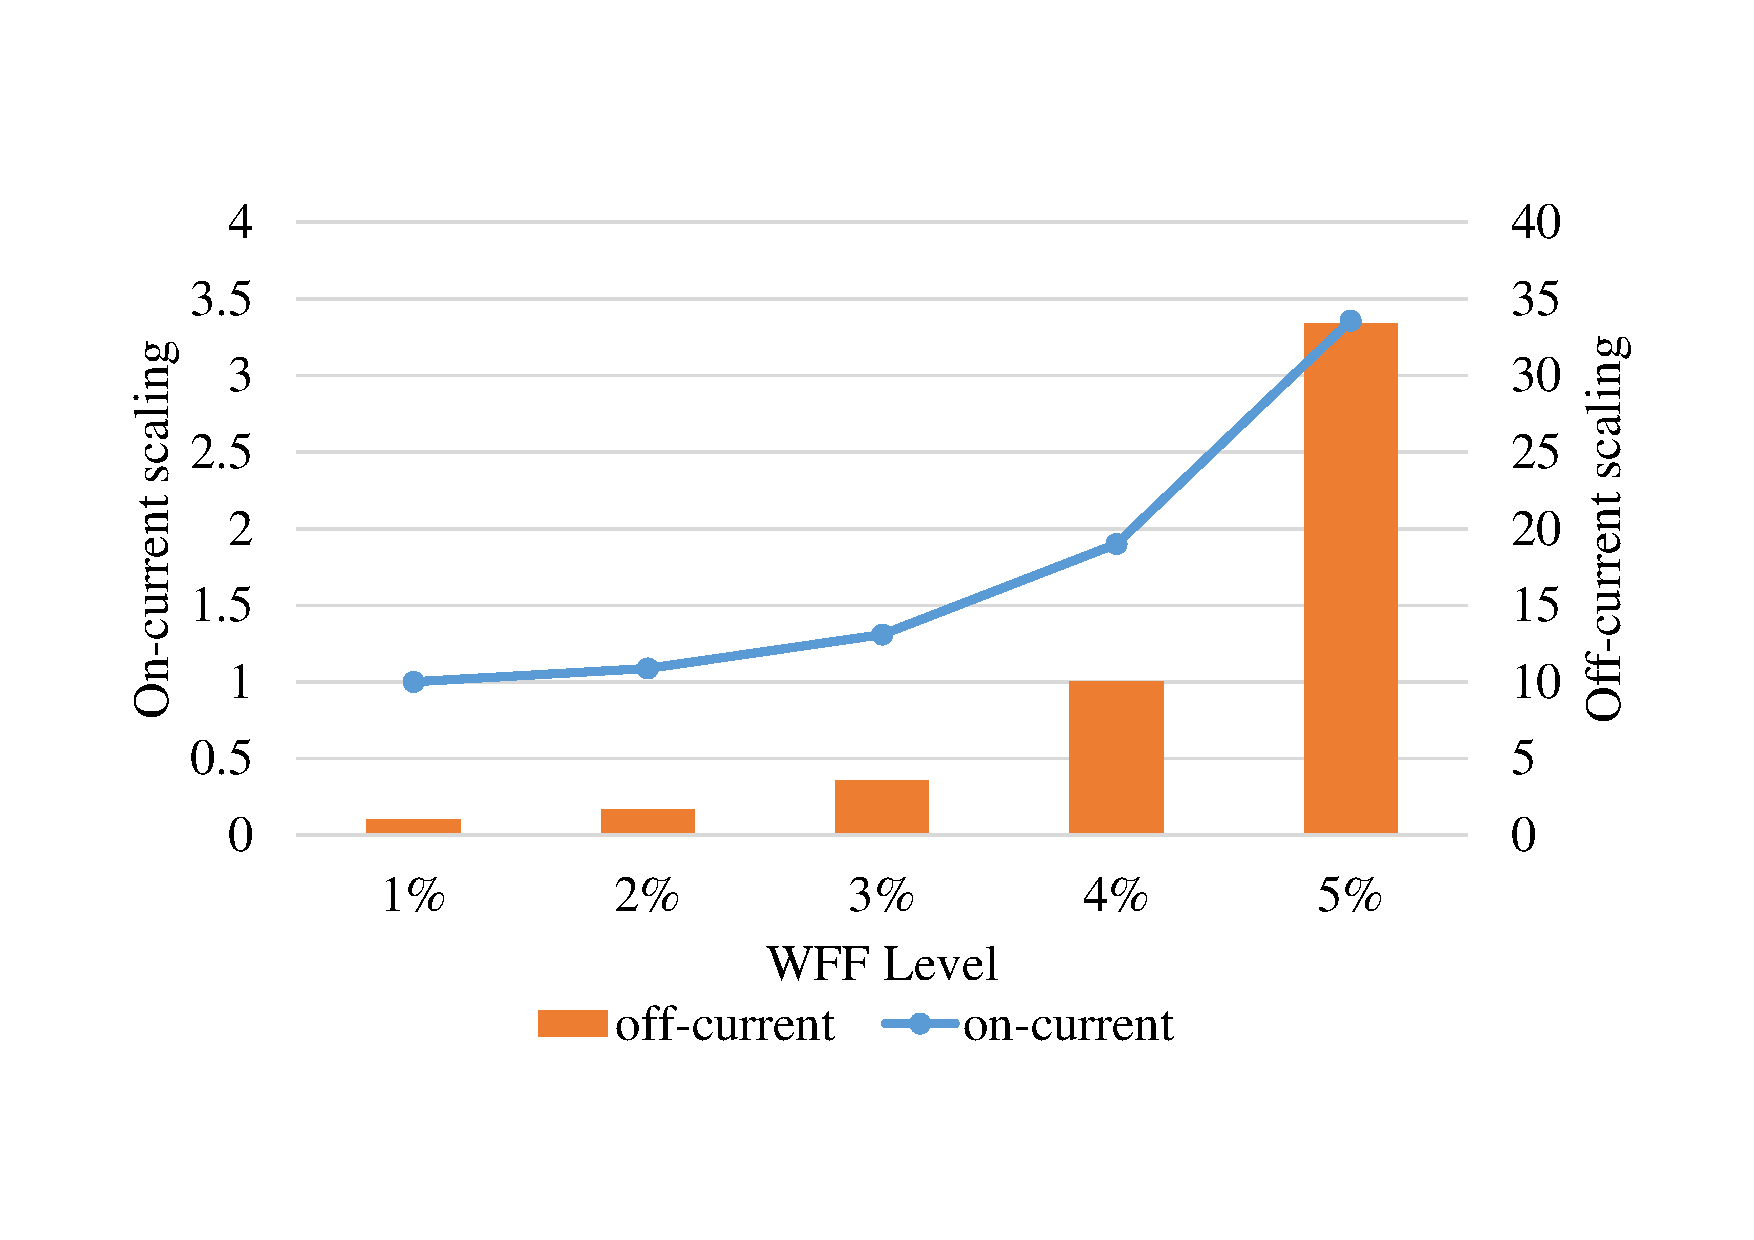
\includegraphics[width=1\textwidth, trim={1.25cm 3cm 2cm 3cm}, clip]{on-off-scaling2.pdf}
            \caption{Average on and off-current increase over all designs through variability scaling. The scaling is normalized in relation to the 1\% WFF level measures.}
        \label{figOnOffScal}
    \end{figure}

    Additionally, it was considered the output gain values for each design, as show in Fig. \ref{figsGainComp}. These measures present the most broader difference across all designs. The TIST and ST designs presented, on average, values up to 8300.60\%, and 1246.50\% higher, respectively, in comparison to the inverter and SIG designs, which presented the same gains. Additionally, the curve slope measures are shown in Fig. \ref{fig:slopes}, where lower slopes can be observed for the TIST, SIG and inverter designs in comparison to the ST. The ST and TIST designs presented 126.24\% and 9.43\% higher average slopes, respectively, in comparison to the inverter and SIG designs which showed identical measures. Figs. \ref{fig:vtcs01} and \ref{fig:vtcs07} show the VTC curves for all designs. It shows how the TIST although presenting higher gain, present lower slopes, given that it takes more time to properly discharge.

    \begin{figure}[]
        \centering
            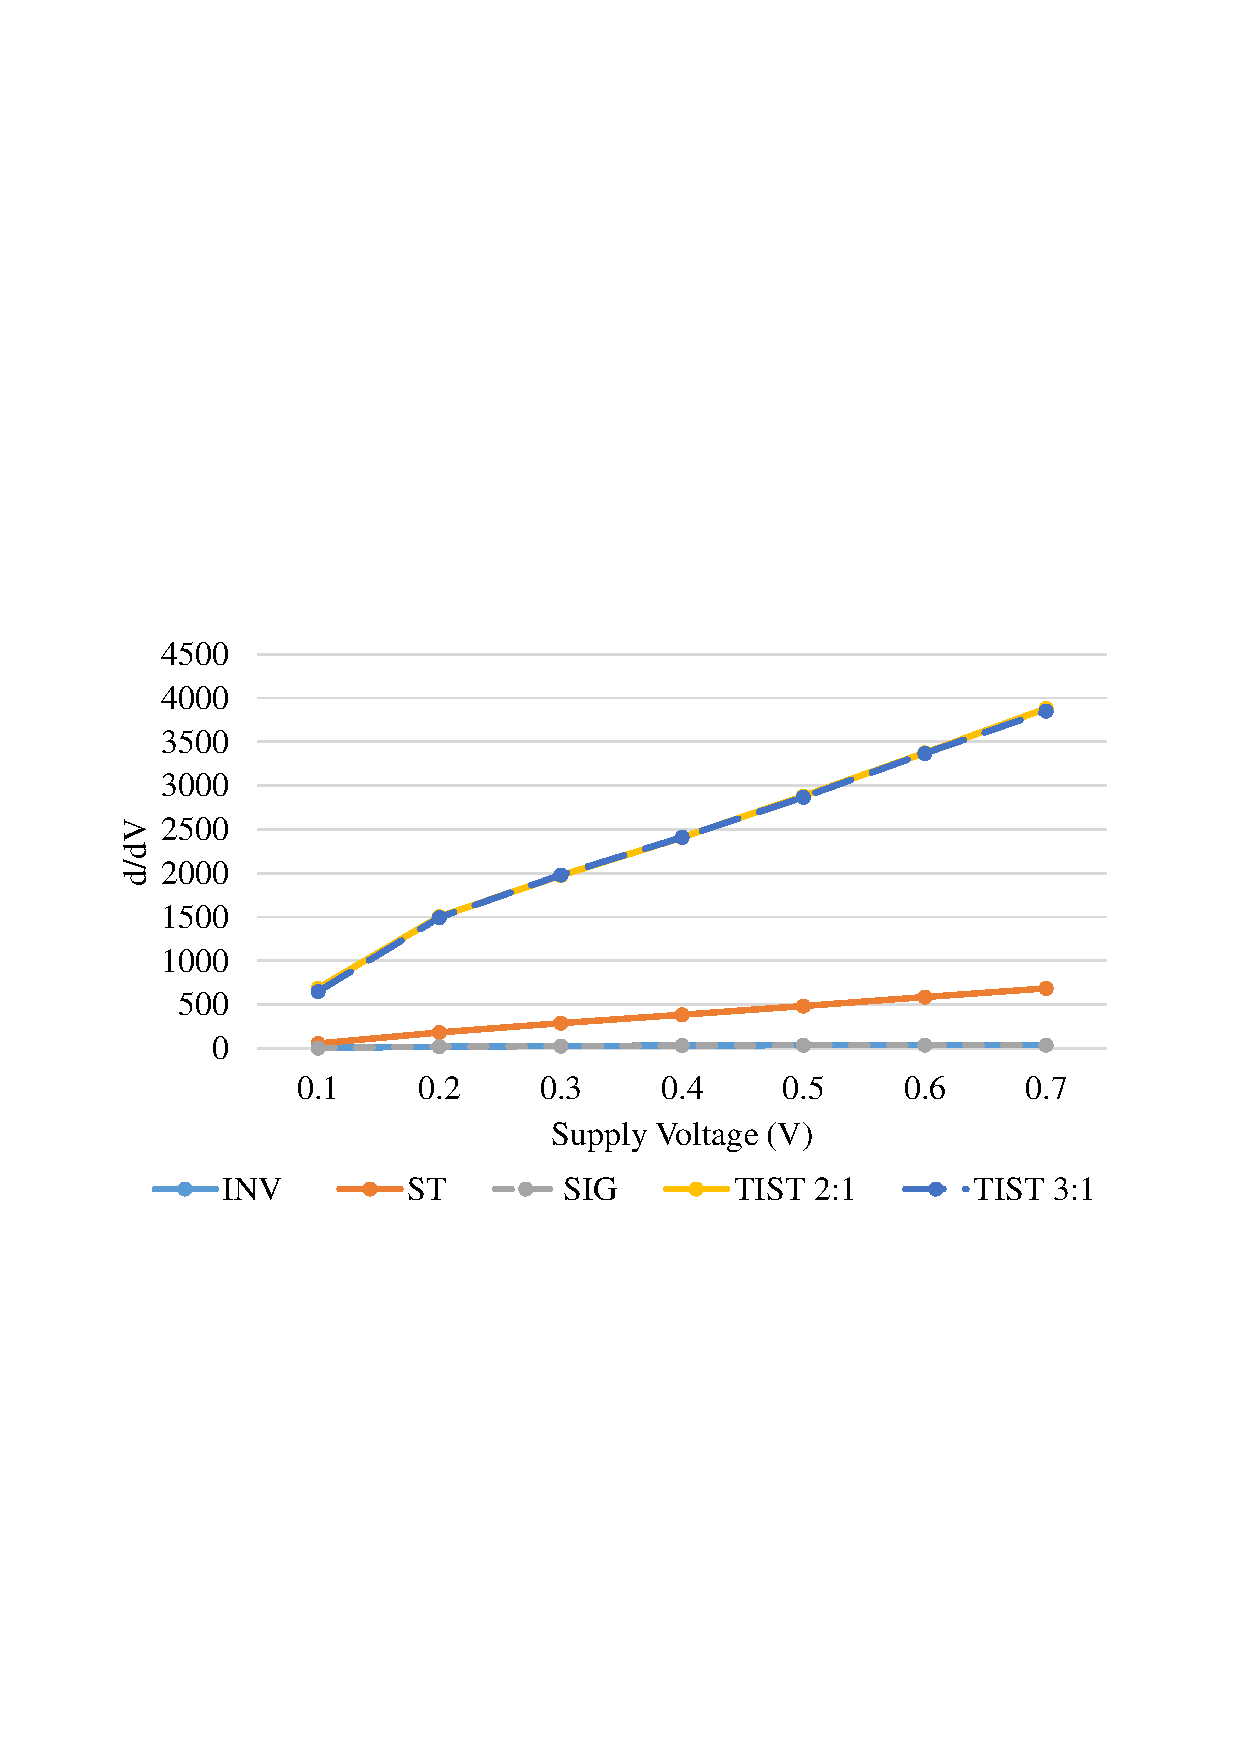
\includegraphics[width=1\textwidth, trim={1.25cm 9cm 2cm 10cm}, clip]{gainComp.pdf}
            \caption{Output gain value across voltage scaling.}
        \label{figsGainComp}
    \end{figure}

    \begin{figure}[]
        \centering
            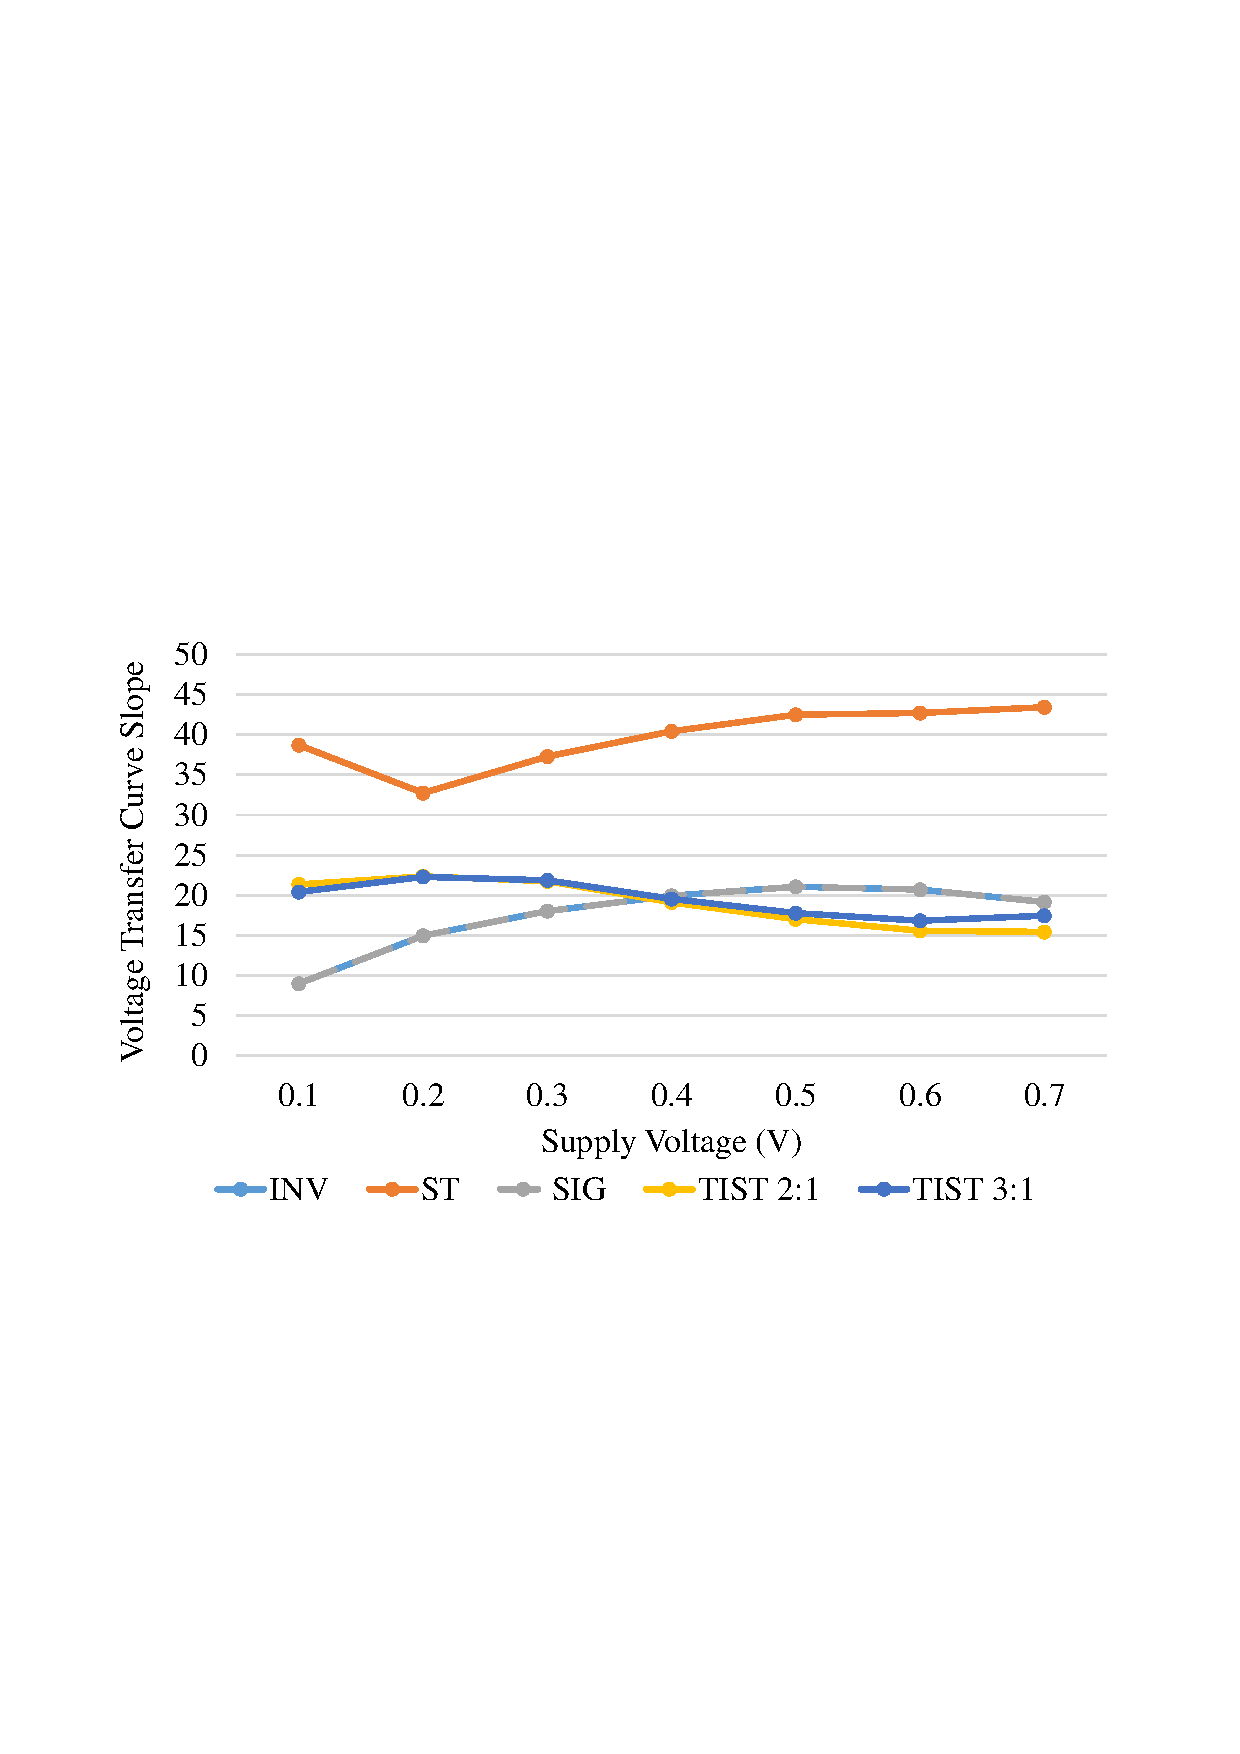
\includegraphics[width=1\textwidth, trim={1.25cm 9cm 2cm 10cm}, clip]{slopes.pdf}
            \caption{Voltage Transfer Curve slopes through supply voltage scaling for each design.}
        \label{fig:slopes}
    \end{figure}

    \begin{figure}[]
        \centering
            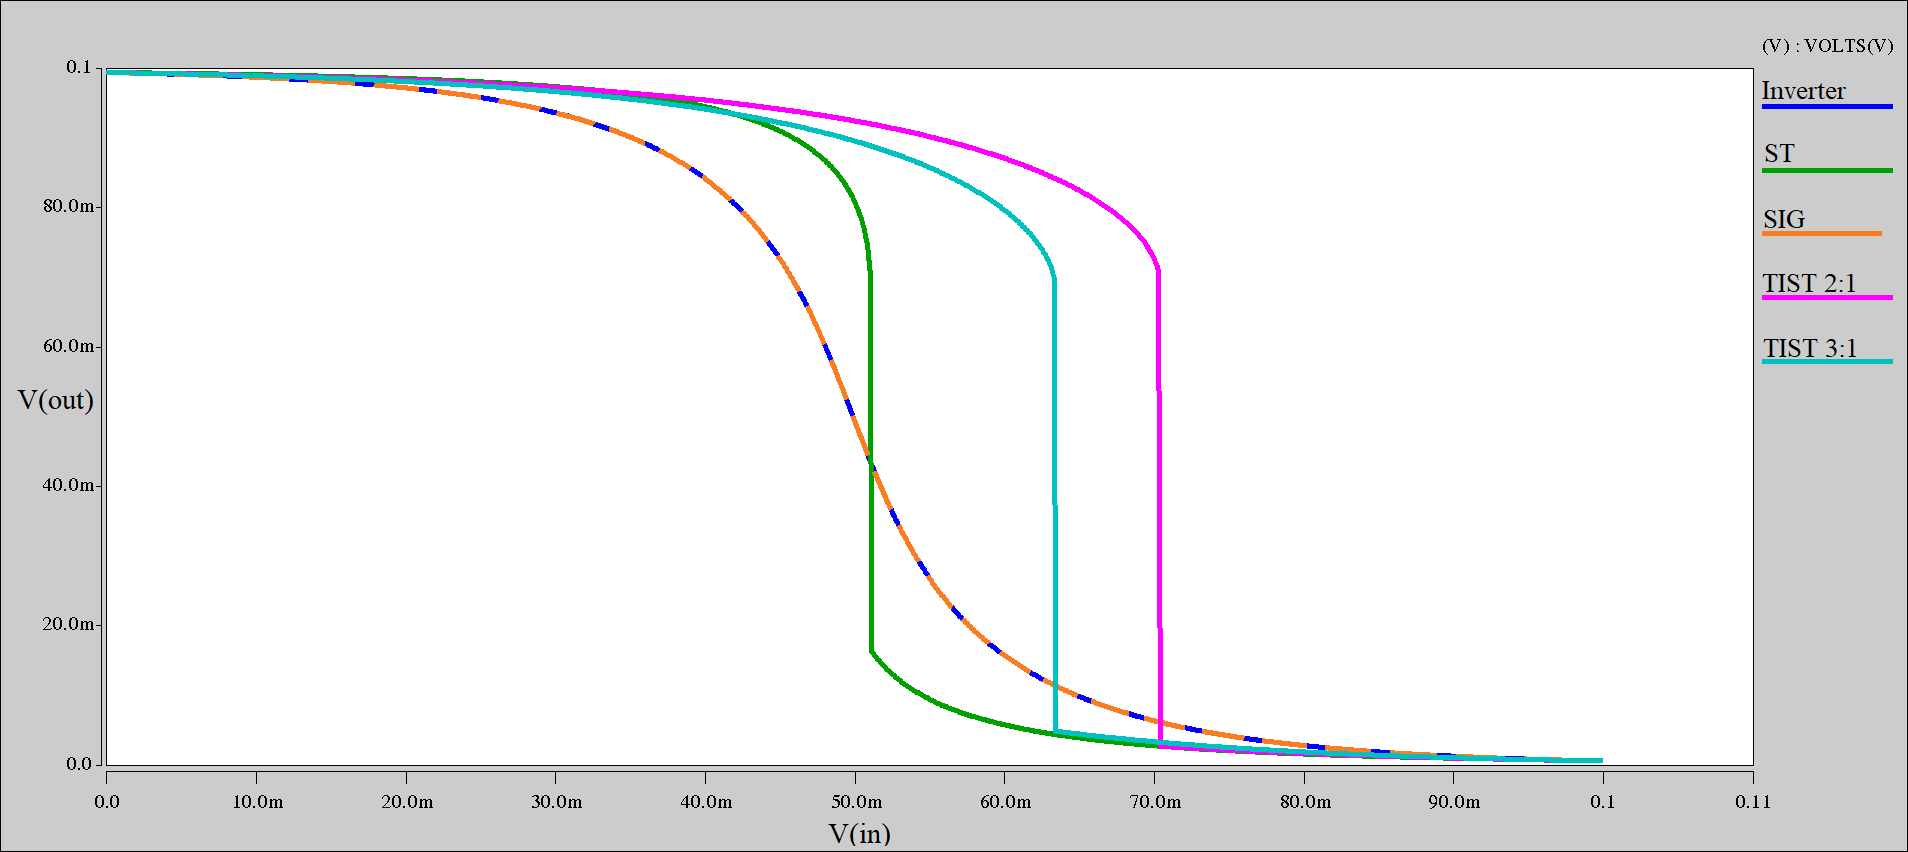
\includegraphics[width=1\textwidth, trim={0cm 0cm 0cm 0cm}, clip]{vtcs01.png}
            \caption{Voltage Transfer Curves for all designs at 0.1V.}
        \label{fig:vtcs01}
    \end{figure}

        \begin{figure}[]
        \centering
            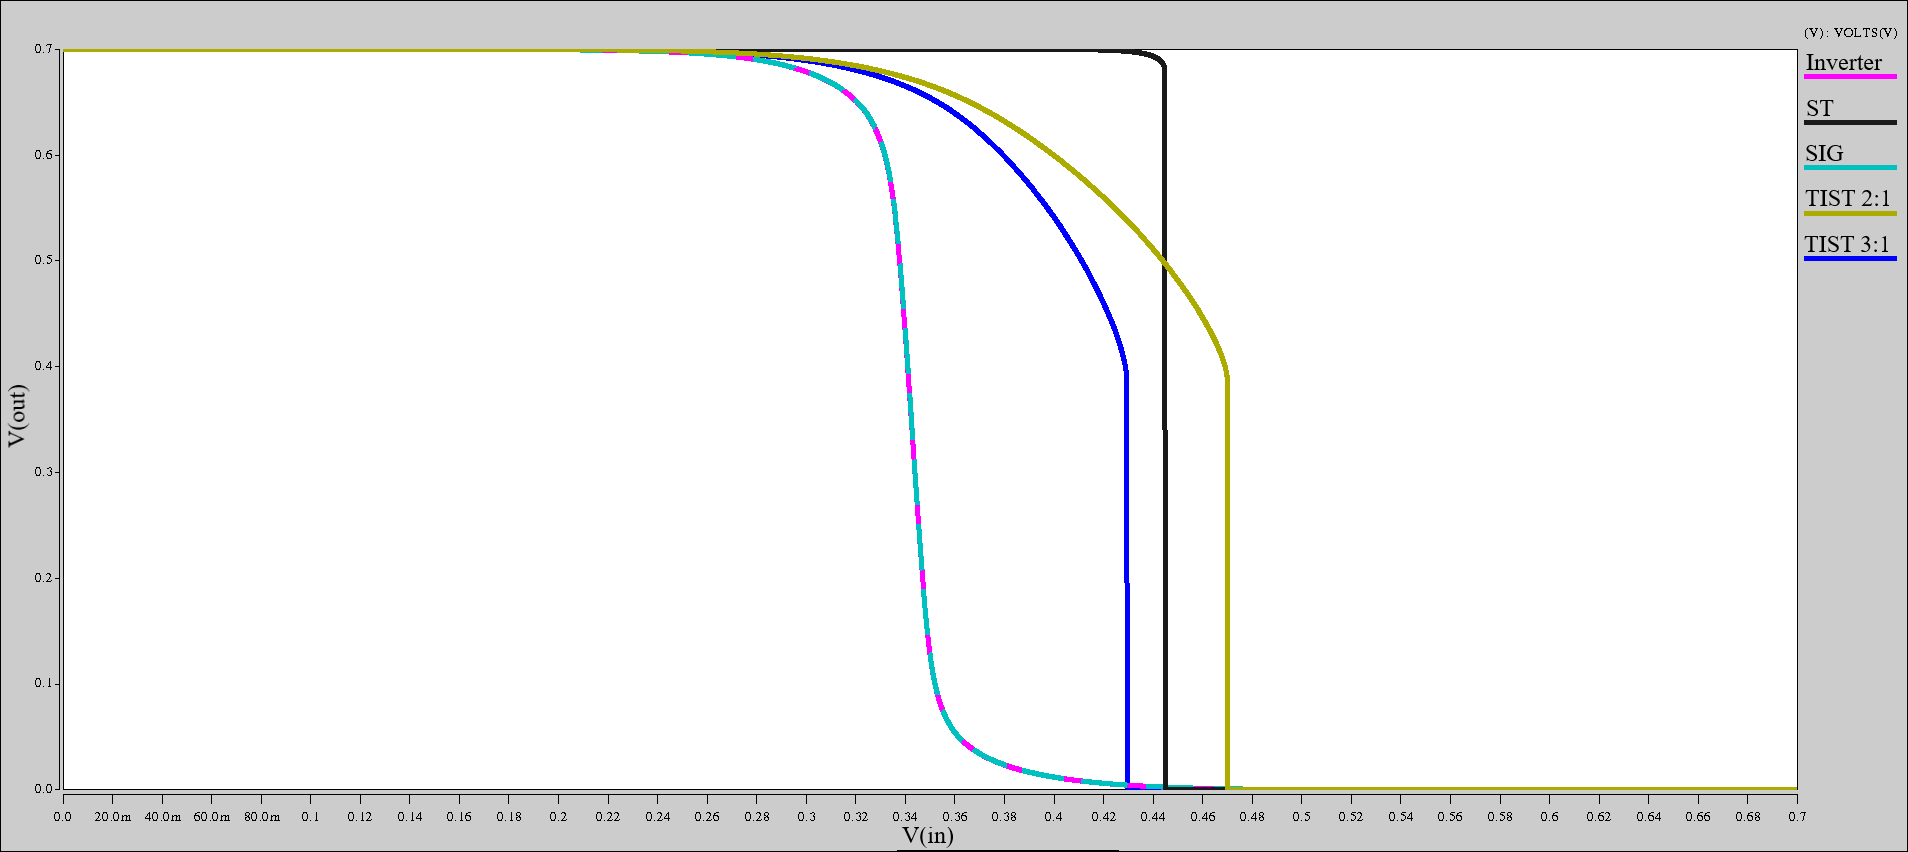
\includegraphics[width=1\textwidth, trim={0cm 0cm 0cm 0cm}, clip]{vtcs07.png}
            \caption{Voltage Transfer Curves for all designs at 0.7V.}
        \label{fig:vtcs07}
    \end{figure}
    %According to \cite{henzler2006power}

    The hysteresis ratios of all designs which present the hysteresis characteristic are shown in Fig. \ref{figsHystComp}. The hysteresis ratio is the ratio between the hysteresis interval (V) and the supply voltage (V), which will result in a percentage of the current supply voltage. Given so, the TIST designs presented higher average ratios of 18.92\% and 15.95\% for the 2:1 and 3:1 designs, respectively, with the ST presenting a ratio average of 8.62\%. It is important to highlight the ratio losses as well, the TIST designs presented ratio decreases up to 14.68\% and the ST presented a better response with a 5.68\% decrease. The hysteresis curves for all designs at nominal supply voltage are shown in Fig. \ref{fig:hystCurves}. Furthermore, the hysteresis ratios in relation to the supply voltage are shown in Fig. \ref{fig:hystRatiosVdd}, it can be observed huge hysteresis intervals for the TIST designs, which are responsible for the circuits failures at working at acceptable frequencies. 

%por que diminui? 

%since due to the variability scaling and its related increase on off-current, the ratios will tend to decrease. This result is due to the leakage current supression embedded into the ST design through the feed-back system. Therefore,
%In order to tackle this problem, further increase of the ratio between the TIST inverter and latch transistors sizes would be necessary, inserting even higher area penalties.

    \begin{figure}[]
        \centering
            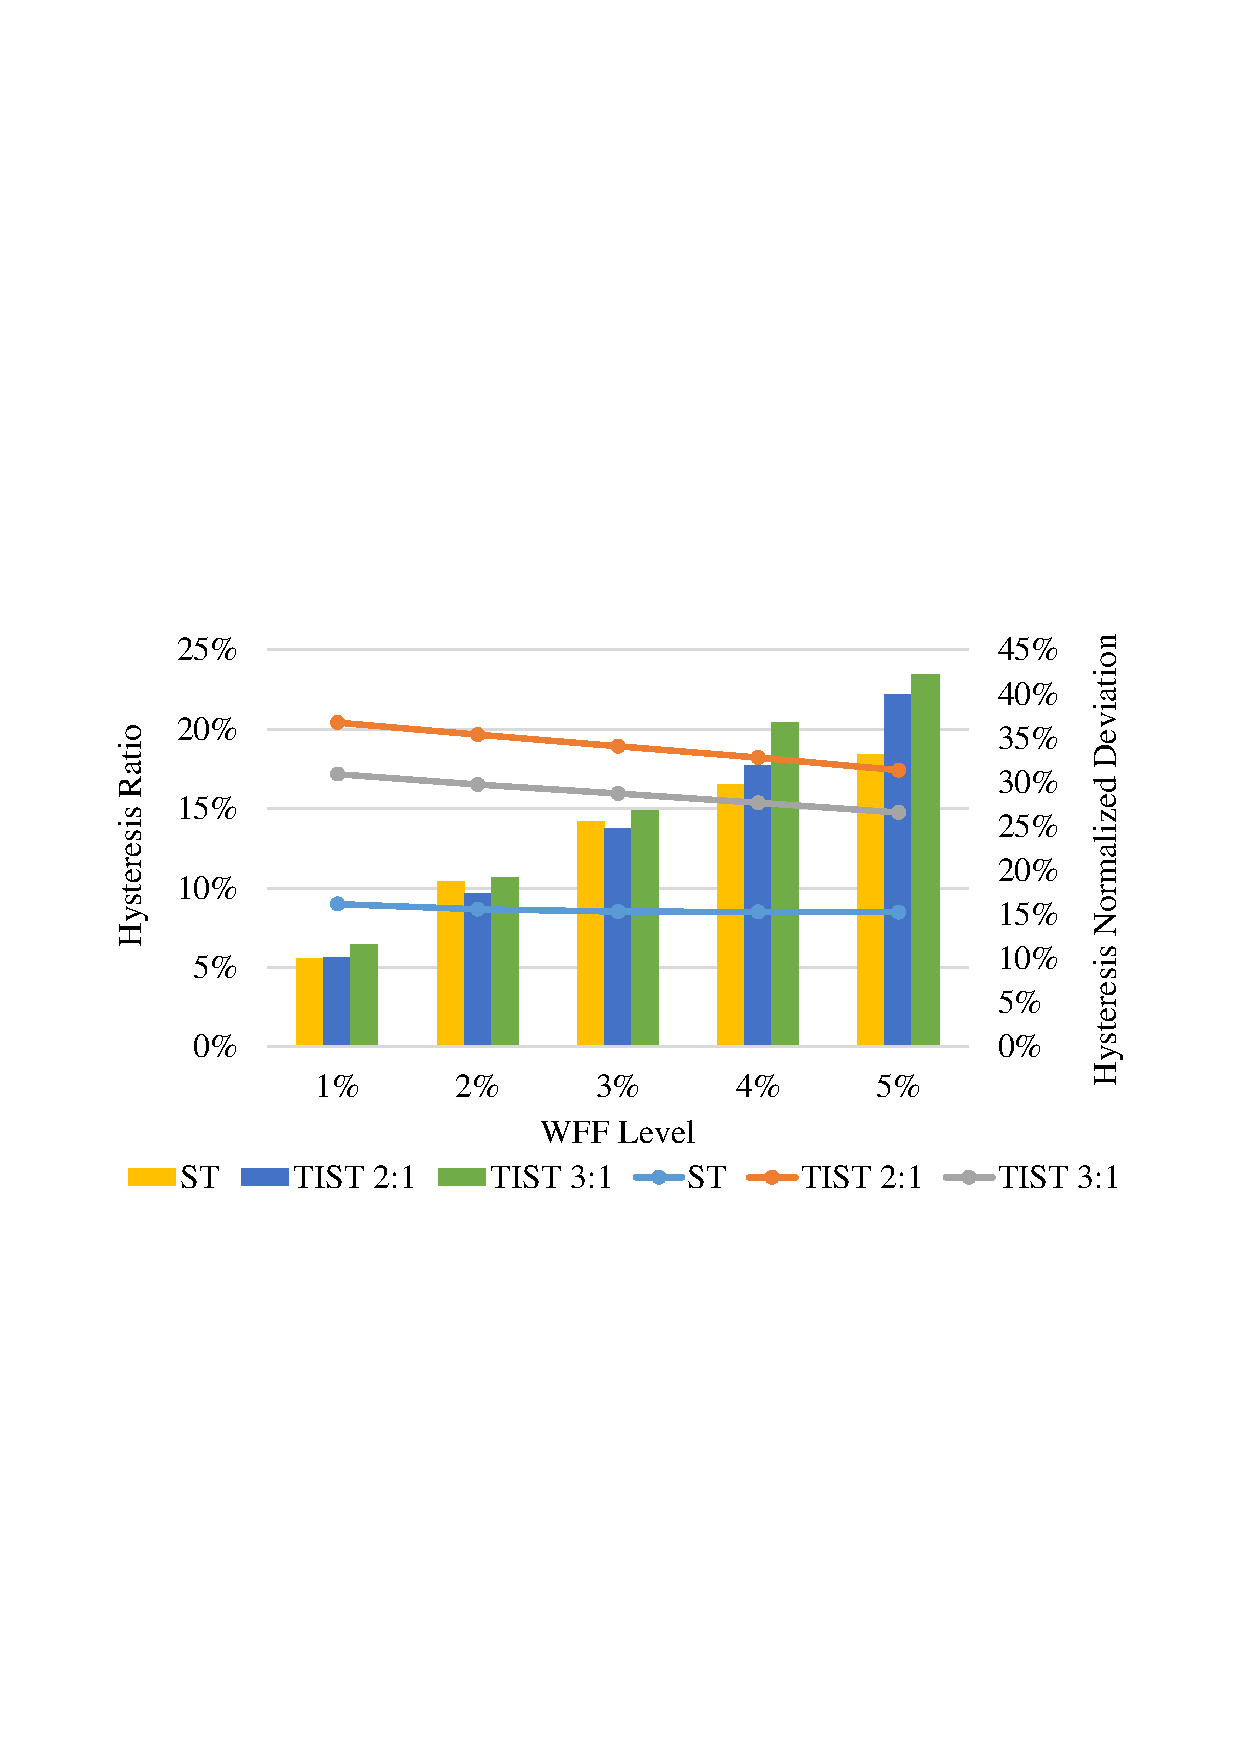
\includegraphics[width=1\textwidth, trim={1.25cm 9cm 2cm 10cm}, clip]{hystWFFComp.pdf}
            \caption{Design hysteresis ratio comparison (left) and hysteresis ratio normalized deviation (right), across variability scaling.}
        \label{figsHystComp}
    \end{figure}

    \begin{figure}[]
        \centering
            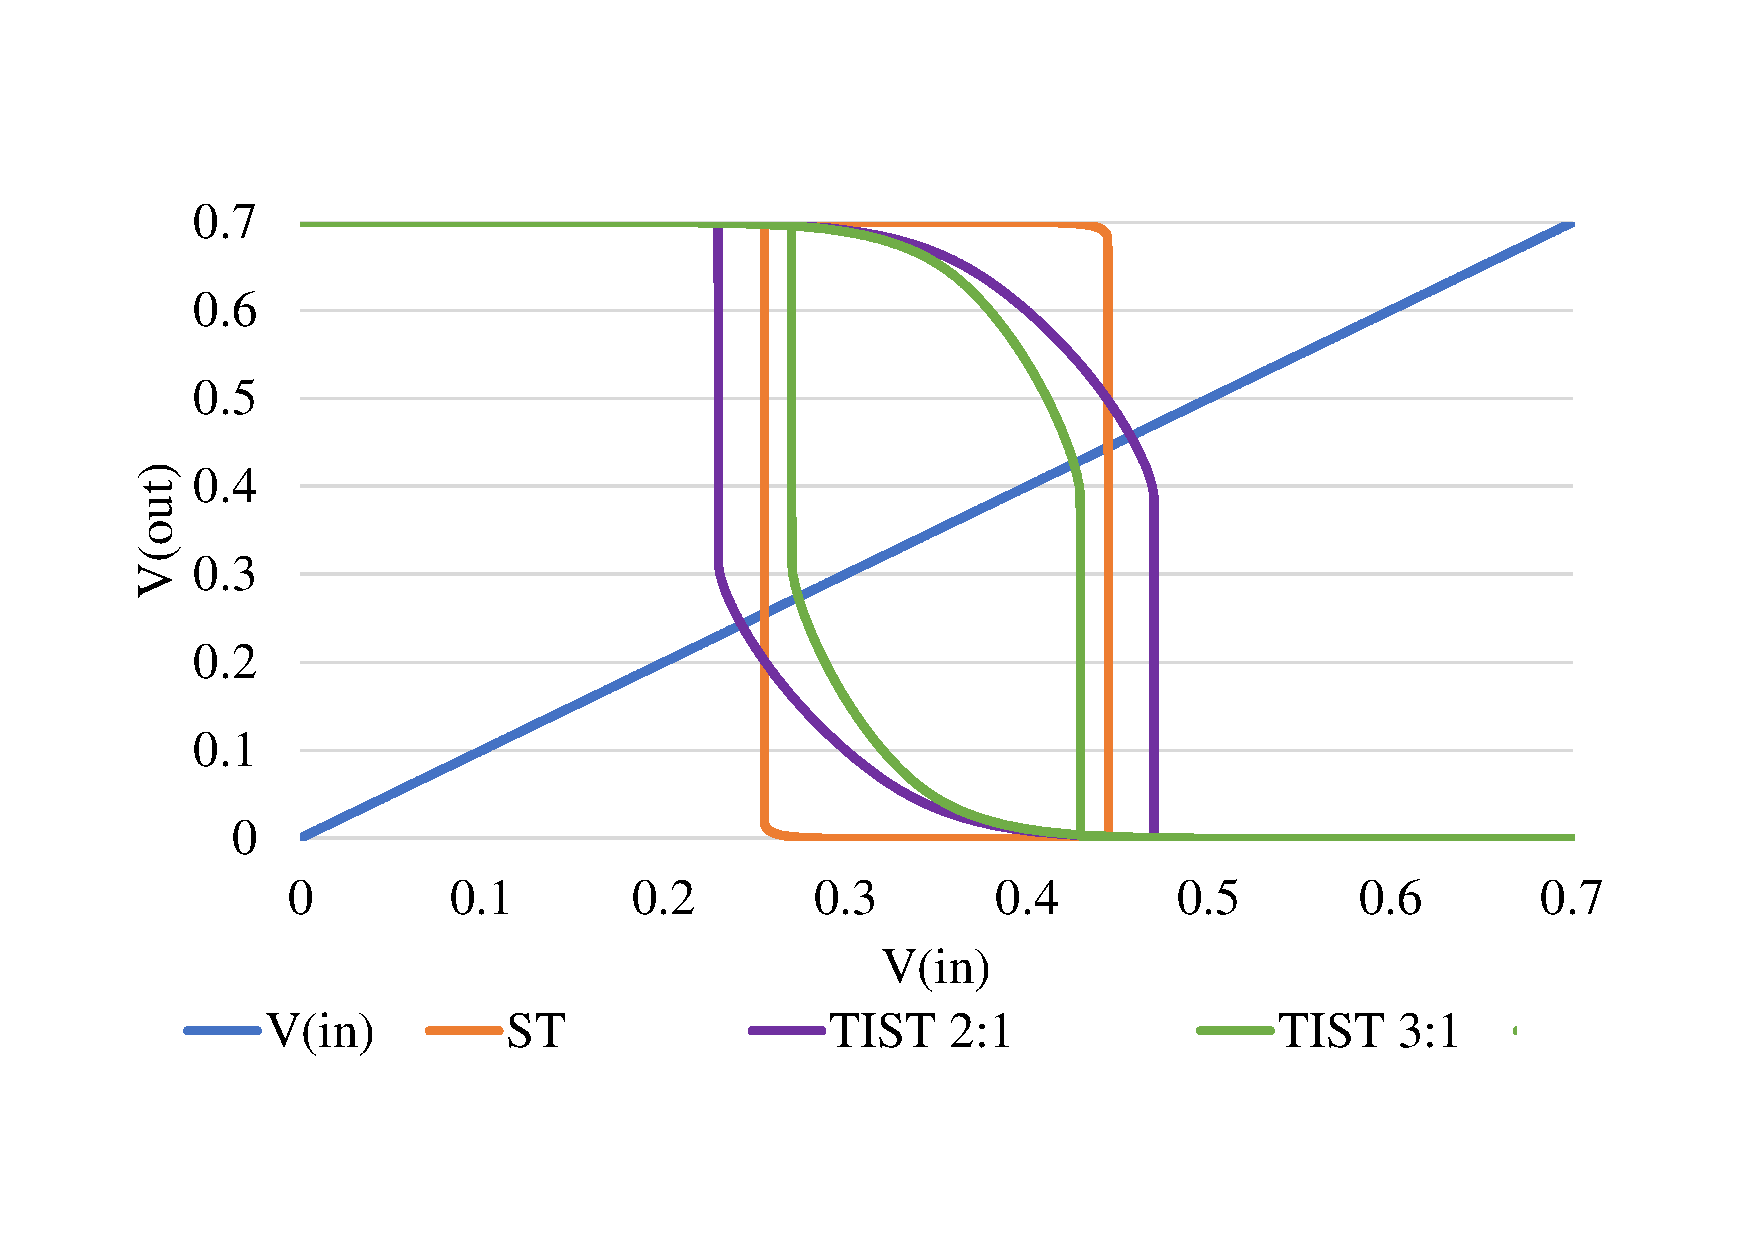
\includegraphics[width=1\textwidth, trim={2cm 3cm 2cm 3cm}, clip]{hystGraphs.pdf}
            \caption{Hysteresis curves for all designs at nominal supply voltage.}
        \label{fig:hystCurves}
    \end{figure}

    \begin{figure}[]
        \centering
            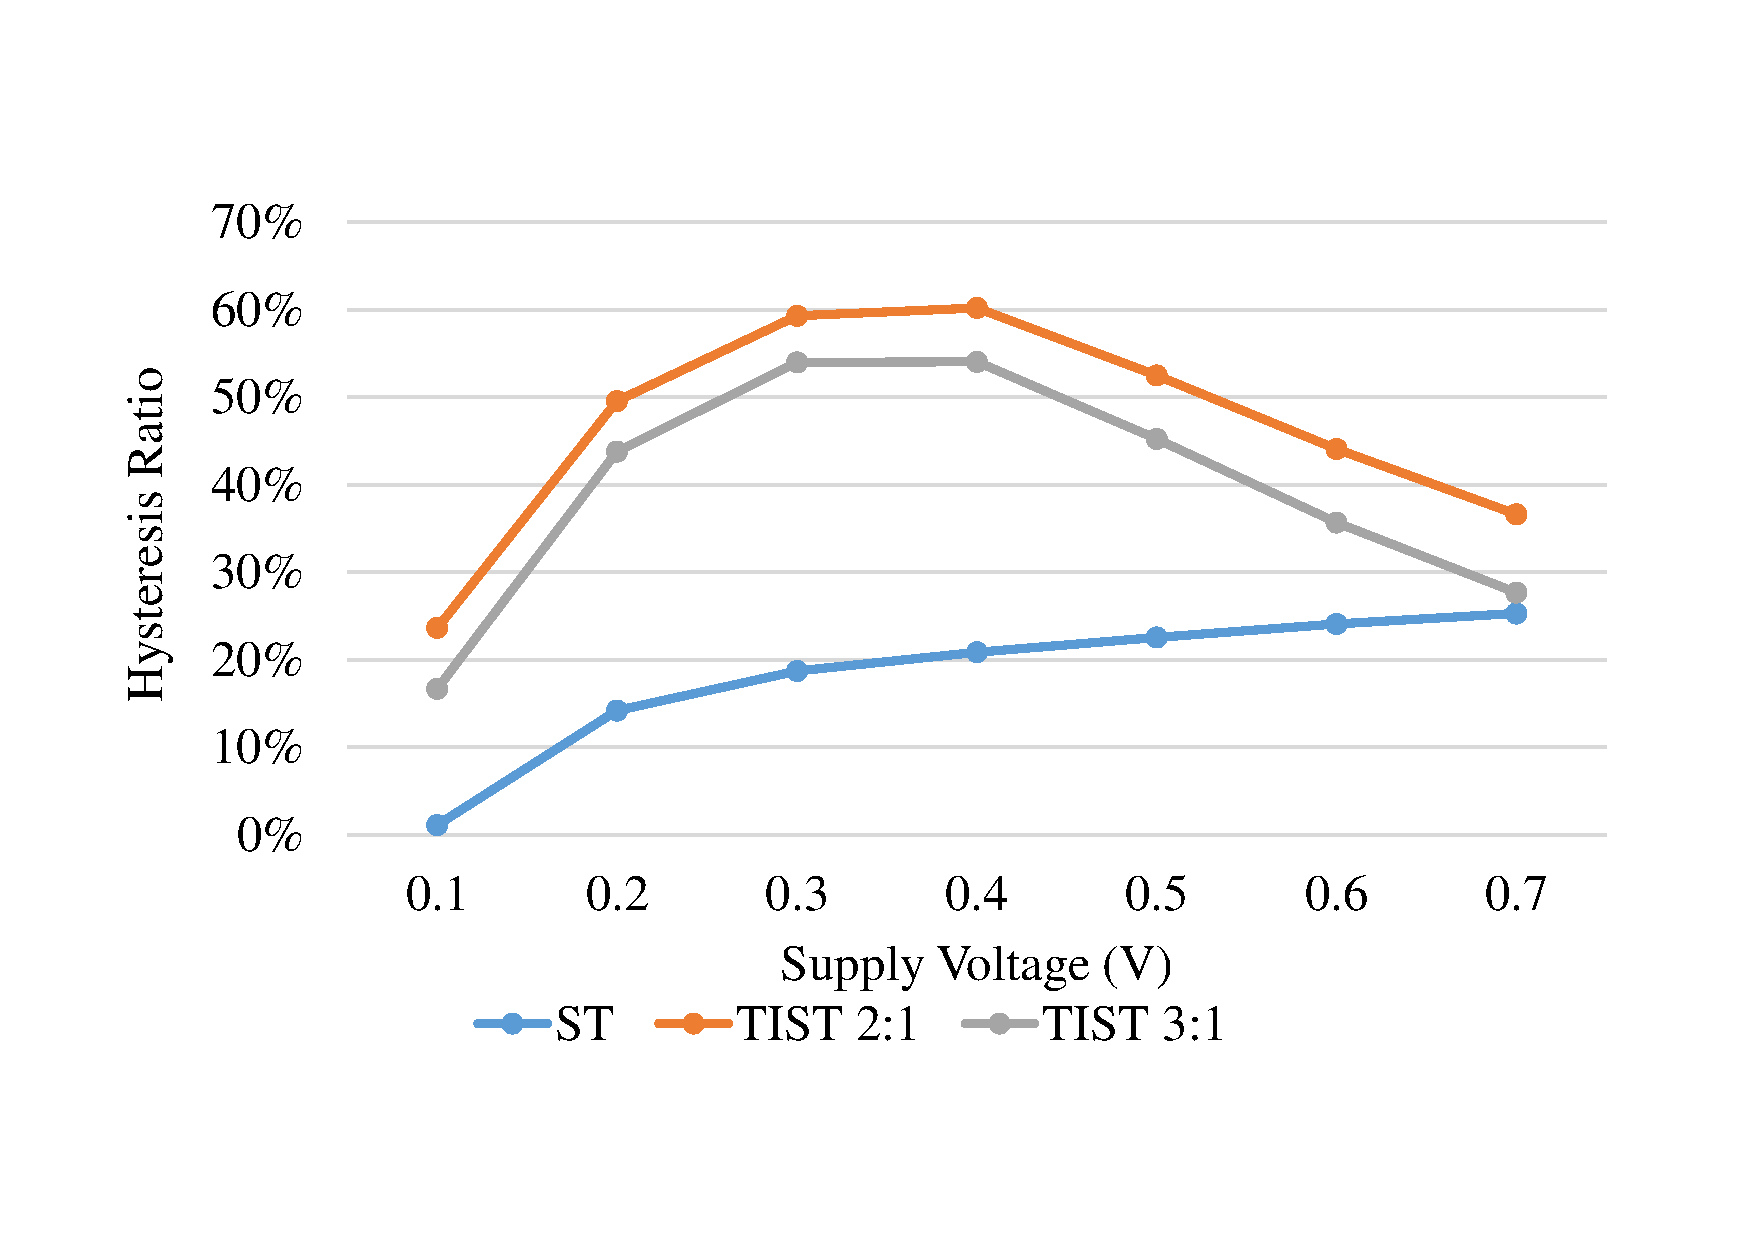
\includegraphics[width=1\textwidth, trim={2cm 3cm 2cm 3cm}, clip]{hystRatiosVdd.pdf}
            \caption{Design hysteresis ratios comparison across supply voltage scaling.}
        \label{fig:hystRatiosVdd}
    \end{figure}

    The average hysteresis ratio deviations for each design was 23.44\%, 24.83\%, and 27.30\% for the ST, TIST 2:1 and TIST 3:1. The hysteresis average ratio deviation measures did not present considerable differences between designs, although, at high variability scenarios (5\% WFF) the ST presented 16.79\% and 21.40\% lower deviations, in comparison to the TIST 2:1 and TIST 3:1, respectively.

    Figs. \ref{fig:energyDist0_2}, \ref{fig:energyDist0_4}, and \ref{fig:energyDist0_7}, show the distribution of the energy metrics for the inverter over all levels of WFF for 0.2V, 0.4V, and 0.7V supply voltages. For low variability and high supply voltage scenarios it can be observed a normal distribution. While at higher variability and lower supply voltages, a left skew can be noted at first where the majority of the cases stay clustered and as soon as the variability rises, the skew will tend to the left, with extreme cases up to 5 orders of magnitude higher than the mean. Hystograms and dispersion graphs for all designs, are shown in Annex C.

     \begin{figure}[]
        \centering
            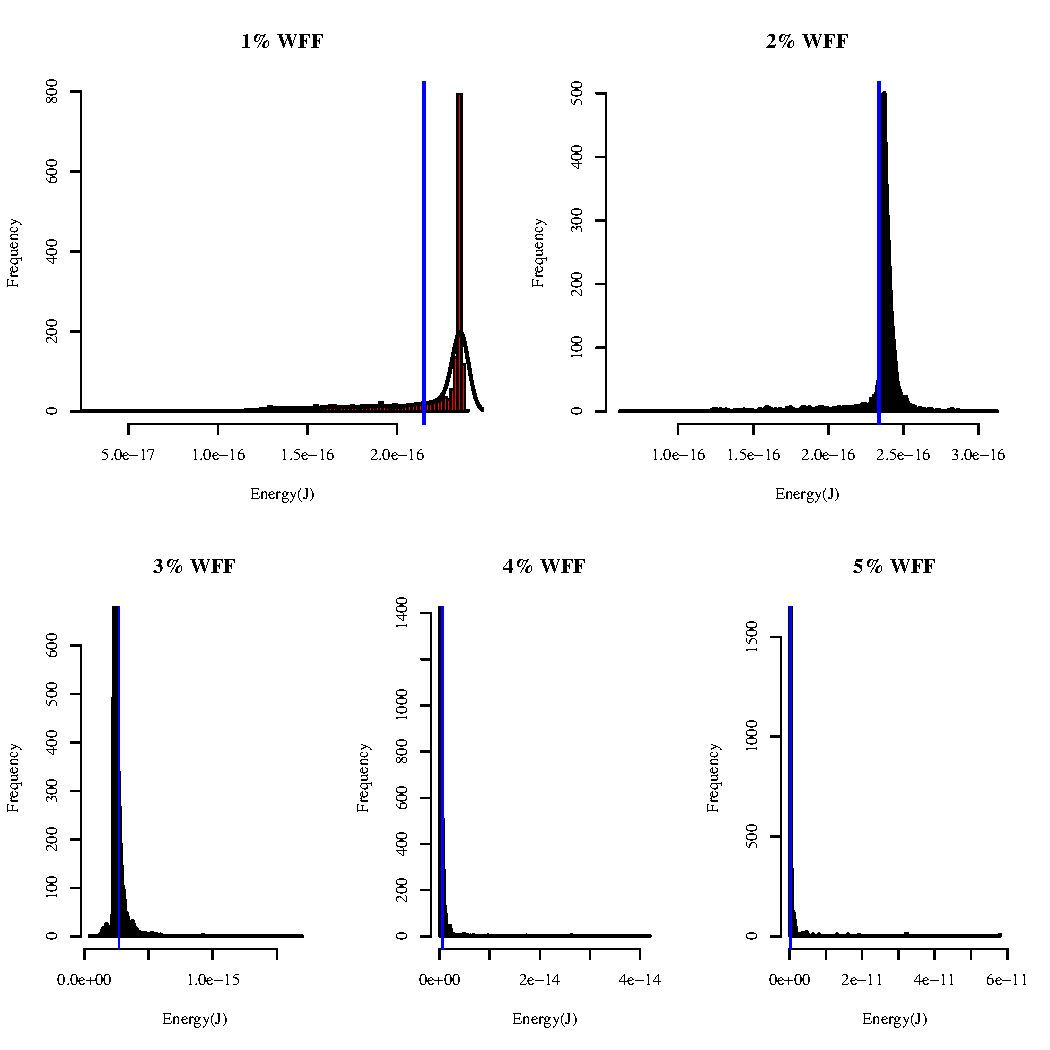
\includegraphics[width=1\textwidth, trim={0cm 0cm 0cm 0cm}, clip]{dist_energy_INV_0_2.pdf}
            \caption{Energy measures distribution for the inverter at different levels of variability at 0.2V.}
        \label{fig:energyDist0_2}
    \end{figure}

    \begin{figure}[]
        \centering
            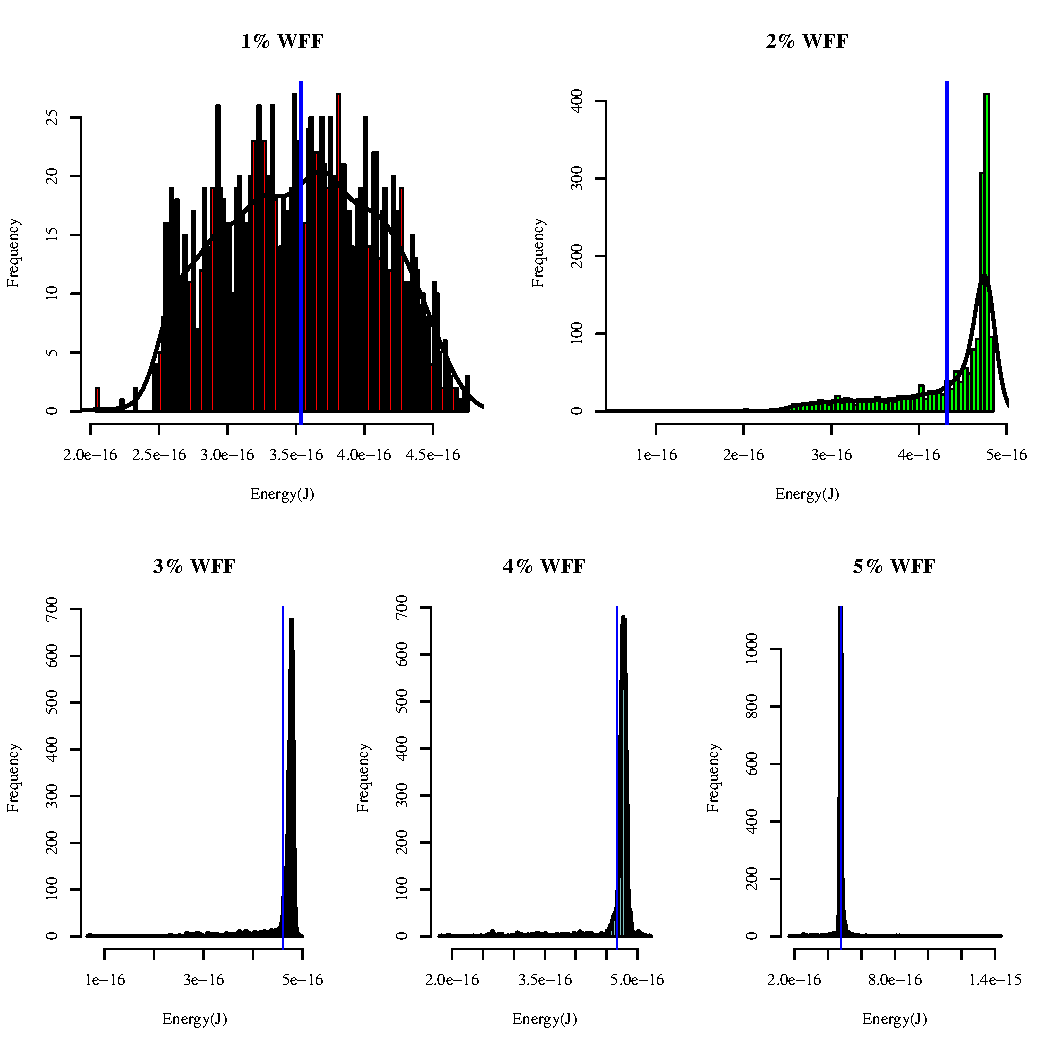
\includegraphics[width=1\textwidth, trim={0cm 0cm 0cm 0cm}, clip]{dist_energy_INV_0_4.pdf}
            \caption{Energy measures distribution for the inverter at different levels of variability at 0.4V.}
        \label{fig:energyDist0_4}
    \end{figure}

         \begin{figure}[]
        \centering
            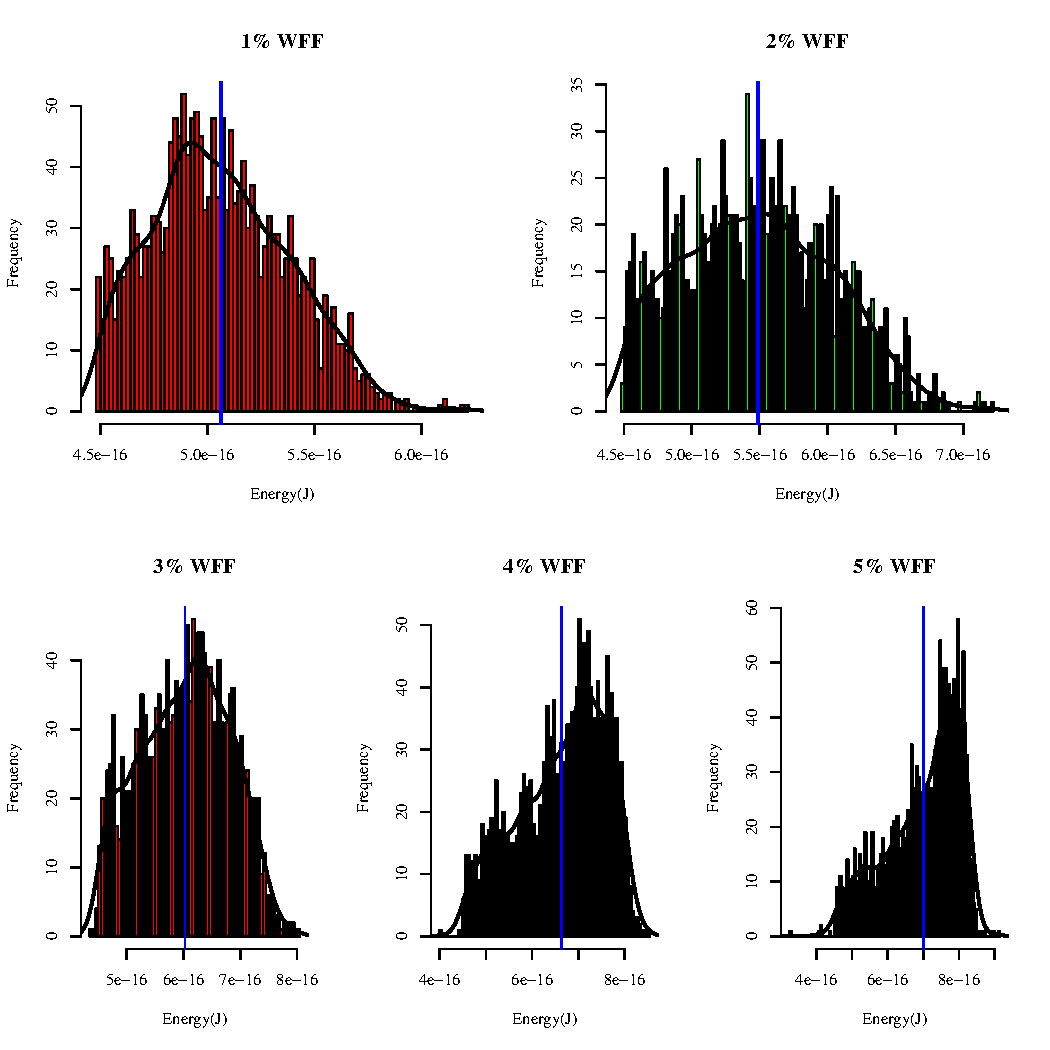
\includegraphics[width=1\textwidth, trim={0cm 0cm 0cm 0cm}, clip]{dist_energy_INV_0_7.pdf}
            \caption{Energy measures distribution for the inverter at different levels of variability at 0.7V.}
        \label{fig:energyDist0_7}
    \end{figure}

\section{Over ST technique applied on Full Adders}

The results are divided into two main analyses, with the set of FAs operating at nominal and near-threshold. In both cases, simulations were performed with and without the ST technique. To better present the improvements (positive values) and drawbacks (negative values) of each ST, results also show a comparison ($\Delta$) between the normalized deviation between the traditional and the circuits with the applied technique. For the sake of simplicity the LPST and traditional 6T ST were renamed ST1 and ST2, respectively.

\subsection{Nominal Operation}

The results concerning propagation times at nominal levels are show in Table \ref{delayNominal}. It is possible to observe no considerable improvement over variability robustness concerning the propagation times. It can be explained due to the pass-transistor logic present in the TFA, TGA, and Hybrid given further signal degradation as a result of the area increase. Furthermore, it can be observed only a slight improvement over the Mirror FA given its mirroring-based logic with many paths to source and ground.

For the energy results, it was observed considerable improvement over robustness in the Mirror, TFA, and TGA, as shown in Table \ref{energiaNominal}. There was a considerable worsening over the Hybrid energy robustness. It is mainly due to its number of transistors, which is comparable to the Mirror FA but it is not entirely based on complementary logic, and the number of internal inverters replaced, further increasing its area and signal degradation. Overall, the traditional TFA presented the best performance and, by far, the lowest energy consumption and energy normalized deviation at nominal operation. However, it presented the highest delay deviations.

%\setlength\tabcolsep{2 pt}

%%DELAYS NOMINAL
\begin{table}[]
\centering
\caption{Delay measures for nominal voltage operation}
\label{delayNominal}
\resizebox{\textwidth}{!}{%
\begin{tabular}{lccccccccc}
\hline
\multirow{3}{*}{FA} & \multirow{3}{*}{ST} & \multicolumn{8}{c}{Delays} \\ \cline{3-10}
 & &  \multicolumn{4}{c}{SUM} & \multicolumn{4}{c}{CARRY OUT} \\ \cline{3-10}
 & & \textbf{$\mu$(ps)} & \textbf{$\sigma$(ps)} & \textbf{$\sigma$/$\mu$(\%)} & \textbf{$\Delta$(\%)} & \textbf{$\mu$(ps)} & \textbf{$\sigma$(ps)} & \textbf{$\sigma$/$\mu$(\%)} & \textbf{$\Delta$(\%)} \\ \hline
\multirow{3}{*}{Mirror} & - & 22.83 & 4.82 & 20.89 & - & 22.60 & 4.39 & 19.38 & - \\ \cline{2-10}
 & ST1 & 27.38 & 5.75 & 20.77 & 0.54 & 25.31 & 4.79  & 18.87 & 2.63 \\ \cline{2-10}
 & ST2 & 42.28 & 8.57 & 20.23 & 3.13 & 41.48 & 7.96 & 19.17 & 1.10 \\ \hline
\multirow{3}{*}{TFA} & - & 20.76 & 5.51 & 30.69 & - & 19.75 & 4.70 & 25.74 & - \\ \cline{2-10}
 & ST1 & 24.24 & 6.43 & 31.42 & -2.37 & 22.50 & 5.51 & 26.74 & -3.86 \\ \cline{2-10}
 & ST2 & 42.36 & 76.87 & 126.26 & -311.36 & 26.91 & 6.86 & 31.45 & -22.18 \\ \hline
\multirow{3}{*}{TGA} & - & 21.56 & 4.30 & 22.36 & - & 22.96 & 4.70  & 20.46 & - \\ \cline{2-10}
& ST1 & 25.32 & 5.36 & 26.42 & -18.16  & 26.39 & 5.41  & 20.38 & 0.37 \\ \cline{2-10}
& ST2 & 97.92 & 210.62 & 102.35 & -357.80 & 32.80 & 7.85 & 25.70 & -25.63 \\ \hline
\multirow{3}{*}{Hybrid} & - & 24.02 & 5.31 & 21.75 & - & 23.58 & 4.89  & 21.65 & - \\ \cline{2-10}
& ST1 & 60.96 & 64.91 & 92.40 & -324.90 & 42.07 & 21.84 & 34.84 & -60.90 \\ \cline{2-10}
& ST2 & 69.68 & 40.87 & 50.82 & -133.72 & 72.05 & 25.81 & 29.23 & -35.00 \\ \hline
\end{tabular}%
}
\end{table}

%%ENERGIA NOMINAL
\begin{table}[]
\centering
\caption{Energy measures for nominal voltage operation}
\label{energiaNominal}
\resizebox{\textwidth}{!}{%
\begin{tabular}{lccccccccc}
\hline
\multirow{3}{*}{FA} & \multirow{3}{*}{ST} & \multicolumn{8}{c}{Energy} \\ \cline{3-10}
 & & \multicolumn{4}{c}{SUM} & \multicolumn{4}{c}{CARRY OUT} \\ \cline{3-10}
 & & \textbf{$\mu$(fJ)} & \textbf{$\sigma$(fJ)} & \textbf{$\sigma$/$\mu$(\%)} & \textbf{$\Delta$(\%)} & \textbf{$\mu$(fJ)} & \textbf{$\sigma$(fJ)} & \textbf{$\sigma$/$\mu$(\%)} & \textbf{$\Delta$(\%)} \\ \hline
\multirow{3}{*}{Mirror} & - & 19.30 & 3.55 & 18.35 & - & 27.30 & 3.99 & 14.60 & - \\ \cline{2-10}
& ST1 & 26.80 & 4.85 & 18.10 & 1.37 & 37.20 & 5.54 & 14.87 & -1.84 \\ \cline{2-10}
& ST2 & 36.50 & 5.50 & 15.07 & 17.87 & 50.80 & 6.54 & 12.87 & 11.84 \\ \hline
\multirow{3}{*}{TFA} & - & 4.97 & 1.27 & 25.59 & - & 5.15 & 0.72 & 13.91 & - \\ \cline{2-10}
& ST1 & 10.90 & 1.46 & 13.38 & 47.70 & 10.80 & 0.98 & 9.09 & 34.68 \\ \cline{2-10}
& ST2 & 17.00 & 2.02 & 11.94 & 53.35 & 15.30 & 2.02 & 13.21 & 5.05 \\ \hline
\multirow{3}{*}{TGA} & - & 14.10 & 3.81 & 27.07 & - & 15.70 & 4.44 & 28.20 & - \\ \cline{2-10}
& ST1 & 24.90 & 6.33 & 25.46 & 5.95 & 26.40 & 4.21 & 15.94 & 43.48 \\ \cline{2-10}
& ST2 & 32.40 & 7.49 & 23.16 & 14.44 & 37.60 & 7.35 & 19.53 & 30.74 \\ \hline
\multirow{3}{*}{Hybrid} & - & 19.30 & 4.10 & 21.26 & - & 26.30 & 4.55 & 17.29 & - \\ \cline{2-10}
& ST1 & 72.50 & 37.95 & 52.34 & -146.19 & 94.60 & 48.21 & 50.94 & -194.62 \\ \cline{2-10}
& ST2 & 73.20 & 21.25 & 29.05 & -36.64 & 95.20 & 19.89 & 20.90 & -20.88 \\ \hline
\end{tabular}%
}
\end{table}

\subsection{Near-Threshold Operation}

 At near-threshold operation, there is little room for noise margin. Given so, it makes full use of the noise immunity characteristic of the STs, as shown in Table \ref{delayNT}. It can be observed a superior robustness improvement with the ST2, given its smaller area, and consequently, lower signal degradation.
 In the case of the TFA it seems that due to its few paths to source and ground, the higher parasitic capacitance and resistance present in ST2 brings higher deviation, with the ST1 presenting better results.

 For the energy results, shown in Table \ref{energiaNT}, ST1 showed superior robustness improvement for the TFA and TGA, which can be explained by their pass-transistor based logic and the ST1 smaller parasitics, in comparison to the Mirror and Hybrid FAs which showed no improvement whatsoever.

 For the delay results, the Mirror FA showed the lowest means and normalized deviations, which is expected given it is not based on pass-transistor logic, having better driving capabilities. For the energy measures, TFA showed the lowest mean, due to its pass-transistor logic and lower number of transistors. Although, the TFA presented the highest delay normalized deviations. Overall, the TGA showed the lowest normalized deviations in energy and the highest robustness gains concerning delay and energy measures.

%%DELAYS NT
\begin{table}[]
\centering
\caption{Delay measures for near-threshold operation}
\label{delayNT}
\begin{tabular}{lccccccccc}
\hline
\multirow{3}{*}{FA} & \multirow{3}{*}{ST} & \multicolumn{8}{c}{Delays} \\ \cline{3-10}
& & \multicolumn{4}{c}{SUM} & \multicolumn{4}{c}{CARRY OUT} \\ \cline{3-10}
& & \textbf{$\mu$(ps)} & \textbf{$\sigma$(ps)} & \textbf{$\sigma$/$\mu$(\%)} & \textbf{$\Delta$(\%)} & \textbf{$\mu$(ps)} & \textbf{$\sigma$(ps)} & \textbf{$\sigma$/$\mu$(\%)} & \textbf{$\Delta$(\%)} \\ \hline
\multirow{3}{*}{Mirror} & - & 103.49 & 63.18 & 60.95 & - & 91.62 & 55.41 & 59.18 & - \\ \cline{2-10}
& ST1 & 119.98 & 67.63 & 56.09 & 7.97 & 115.50 & 73.68 & 64.11 & -8.32 \\ \cline{2-10}
& ST2 & 155.58 & 67.03 & 42.94 & 29.55 & 153.50 & 68.89 & 44.86 & 24.20 \\ \hline
\multirow{3}{*}{TFA} & - & 122.48 & 117.46 & 111.51 & - & 111.64 & 186.41 & 236.88 & - \\ \cline{2-10}
& ST1 & 142.18 & 146.61 & 97.85 & 12.25 & 118.26 & 194.03 & 242.22 & -2.26 \\ \cline{2-10}
& ST2 & 215.93 & 222.26 & 117.29 & -5.18 & 165.48 & 335.16 & 273.57 & -15.49 \\ \hline
\multirow{3}{*}{TGA} & - & 130.43 & 109.19 & 85.78 & - & 114.78 & 130.53 & 138.93 & - \\ \cline{2-10}
& ST1 & 122.99 & 98.03 & 79.75 & 7.03 & 128.98 & 101.51 & 88.48 & 36.32 \\ \cline{2-10}
& ST2 & 187.84 & 125.13 & 70.99 & 17.25 & 164.06 & 109.19 & 72.68 & 47.68 \\ \hline
\multirow{3}{*}{Hybrid} & - & 115.90 & 83.02 & 70.57 & - & 111.92 & 82.45 & 74.76 & - \\ \cline{2-10}
& ST1 & 187.36 & 143.80 & 78.99 & -11.93 & 116.02 & 71.26 & 61.00 & 18.41 \\ \cline{2-10}
& ST2 & 207.00 & 168.04 & 72.56 & -2.81 & 167.50 & 66.72 & 40.94 & 45.23 \\ \hline
\end{tabular}
\end{table}
\vspace{1em}
%ENERGIA NT

\begin{table}[]
\centering
\caption{Energy measures for near-threshold operation}
\label{energiaNT}
\begin{tabular}{lccccccccc}
\hline
\multirow{3}{*}{FA} & \multirow{3}{*}{ST} & \multicolumn{8}{c}{Energy} \\ \cline{3-10}
& & \multicolumn{4}{c}{SUM} & \multicolumn{4}{c}{CARRY OUT} \\ \cline{3-10}
& & \textbf{$\mu$(fJ)} & \textbf{$\sigma$(fJ)} & \textbf{$\sigma$/$\mu$(\%)} & \textbf{$\Delta$(\%)} & \textbf{$\mu$(fJ)} & \textbf{$\sigma$(fJ)} & \textbf{$\sigma$/$\mu$(\%)} & \textbf{$\Delta$(\%)} \\ \hline
\multirow{3}{*}{Mirror} & - & 10.10 & 3.04 & 30.12 & - & 14.10 & 2.53 & 18.00 & - \\ \cline{2-10}
& ST1 & 13.90 & 4.05 & 29.07 & 3.50 & 18.60 & 4.25 & 22.93 & -27.42 \\ \cline{2-10}
& ST2 & 18.40 & 4.34 & 23.60 & 21.64 & 25.30 & 5.73 & 22.59 & -25.53 \\ \hline
\multirow{3}{*}{TFA} & - & 2.62 & 0.83 & 31.49 & - & 2.71 & 0.37 & 13.49 & - \\ \cline{2-10}
& ST1 & 5.67 & 1.34 & 23.69 & 24.76 & 5.69 & 0.63 & 11.01 & 18.38 \\ \cline{2-10}
& ST2 & 9.69 & 2.11 & 21.74 & 30.96 & 8.80 & 2.59 & 29.40 & -117.89 \\ \hline
\multirow{3}{*}{TGA} & - & 6.87 & 1.56 & 22.68 & - & 8.11 & 2.90 & 35.70 & - \\ \cline{2-10}
& ST1 & 12.90 & 2.37 & 18.45 & 18.65 & 13.50 & 1.86 & 13.79 & 61.37 \\ \cline{2-10}
& ST2 & 16.10 & 3.09 & 19.17 & 15.48 & 17.30 & 2.57 & 14.86 & 58.38 \\ \hline
\multirow{3}{*}{Hybrid} & - & 9.66 & 3.09 & 32.02 & - & 12.80 & 3.17 & 24.77 & - \\ \cline{2-10}
& ST1 & 36.40 & 17.94 & 49.30 & -53.96 & 45.80 & 23.63 & 51.54 & -108.07 \\ \cline{2-10}
& ST2 & 35.40 & 12.72 & 35.91 & -12.14 & 46.60 & 13.84 & 29.69 & -19.86 \\ \hline
\end{tabular}
\end{table}

\vspace{-1.5em}

 \subsection{Penalties}

Overviews for metrics measurements and variability sensitivities are shown in Figs. \ref{fig:avgDelayNominal} to \ref{fig:avgEnergyNT}. Since it was considered a technique where a single inverter (2 transistors) by ST1/ST2 (4/6 transistors). It is expected penalties concerning delay, energy and area metrics. For the delays, it was observed an average 30\% and 97\% increase for the ST1 and ST2, respectively. Additionally, for the energy, there was a 123\% and 176\% average increase for the ST1 and ST2, respectively.

Concerning area penalties, the ST1 increased the FAs area by 157.71\%, on average, while the ST2 increased by 52.20\%. The ST1 higher increase in area is due to the necessity to use TAP-Cells, which is a technology restriction, in order to explicitly connect the transistor's bulk to specific points of the circuit or source/ground making the ST1 cell more prominent than expected. The ST2 does not apply specific bulk connections, although it was necessary the use of METAL3 for cell routing, increasing parasitic capacitance and resistance.

Considering all scenarios, there can be observed no delay robustness improvement at nominal operation with the ST1 and ST2 showing, on average, 50\% and 115.2\% worsening on delay robustness, respectively. For energy robustness, at nominal operation, the ST2 presented a considerable average improvement of 11.18\% while the ST1 showed an average worsening of 25\%. For near-threshold operation, ST1 and ST2 showed 7.79\% and 18.173\% higher delay robustness. For energy robustness, the ST2 showed a 4.13\% improvement while the ST1 presented a worsening of 4.5\%.

%\vspace{-3.65em}

\begin{figure}[]
  \centering
    \includegraphics[width=\textwidth, trim={2cm 10cm 2cm 10.5cm}, clip]{averageDelayNominal.pdf}
     \caption{Average delay measures for nominal operation and their respective normalized deviation (variability sensitivity).}
  \label{fig:avgDelayNominal}
\end{figure}

%\vspace{1em}

\begin{figure}[]
  \centering
    \includegraphics[width=\textwidth, trim={3.5cm 3cm 2cm 3.5cm}, clip]{averageEnergyNominal.pdf}
     \caption{Average energy measures for nominal operation and their respective normalized deviation (variability sensitivity).}
  \label{fig:avgEnergyNominal}
\end{figure}

%\vspace{1em}

\begin{figure}[]
  \centering
    \includegraphics[width=\textwidth, trim={3.5cm 3cm 2cm 3.5cm}, clip]{averageDelayNT.pdf}
     \caption{Average delay measures for near-threshold operation and their respective normalized deviation (variability sensitivity).}
  \label{fig:avgDelayNT}
\end{figure}

%\vspace{1em}

\begin{figure}[]
  \centering
    \includegraphics[width=\textwidth, trim={3.5cm 3cm 2cm 3.5cm}, clip]{averageEnergyNT.pdf}
     \caption{Average energy measures for near-threshold operation and their respective normalized deviation (variability sensitivity).}
  \label{fig:avgEnergyNT}
\end{figure}

\chapter{Conclusions}

The ongoing trend of IoT devices was enabled by two key technology improvements: battery lifetime and capacity improvement, and node scaling. Although, for specific applications, battery maintenance and charging through the power grid is not possible. Given so, IoT devices have been constrained with tight energy consumption metrics, and adapted with self-sufficient mechanisms in order to produce energy through external sources. The node scaling, that enabled IoT devices, comes not short of inherent challenges, with process variability being the major one. New transistor technologies have been proposed such as FinFETs, although even such devices, at deep submicron nodes (e.g. 7-nm), present considerable deviation in its metrics. Such deviations are not appropriate for such sensible devices working at narrow constraints (with energy consumption being a priority).

Given so, an analysis over multiple scenarios considering several levels of process variability, supply voltages, and transistor sizing was performed in order to identify the adequate fin number and supply voltage for various kinds of inverter circuits prioritizing energy consumption and the minimization of deviations. Furthermore, the impact of the replacement of Full Adders internal inverters was analyzed considering two types of Schmitt Trigger and four types of Full Adders.

An overview for the inverter designs analysis is shown in Table \ref{tab:overview}. On performance, the inverter presented the lowest propagation times, and lowest frequency loss due to variability impact. Although, it presented the higher propagation deviations than the ST and SIG designs. The ST and SIG designs presented the lowest frequencies, but lowest propagation times deviations as well. The TIST 2:1 designs presented frequencies on average lower to the ST and SIG designs, and higher deviations, second only to the 3:1 designs which presented higher frequencies, apart from the inverter, than all of the designs. Given so, it can be observed the higher impact of variability on the TIST designs which present the lowest average frequencies (for the 2:1 TISTs) and second highest frequencies (for the 3:1 TISTs) and still presented considerable higher propagation deviations in comparison to all designs.

% Please add the following required packages to your document preamble:
% \usepackage{multirow}
% \usepackage{graphicx}
\begin{table}[]
\centering
\caption{Overall results overview for all designs.}
\label{tab:overview}

\resizebox{0.8\textwidth}{!}{%
\begin{tabular}{|c|c|c|c|}
\hline
Metric                            &         & Absolute     & Deviations \\ \hline
\multirow{2}{*}{Delays}           & Highest & TIST 2:1     & TIST 3:1   \\ \cline{2-4} 
                                  & Lowest  & INV          & SIG        \\ \hline
\multirow{2}{*}{Energy}           & Highest & TIST 2:1     & TIST 2:1   \\ \cline{2-4} 
                                  & Lowest  & INV          & INV        \\ \hline
\multirow{2}{*}{SNMs}             & Highest & ST           & -          \\ \cline{2-4} 
                                  & Lowest  & TIST 2:1     & -          \\ \hline
\multirow{2}{*}{Current Ratios}   & Highest & TIST 2:1     & TIST 2:1   \\ \cline{2-4} 
                                  & Lowest  & SIG          & ST         \\ \hline
\multirow{2}{*}{Gain}             & Highest & TIST         & -          \\ \cline{2-4} 
                                  & Lowest  & INV/SIG      & -          \\ \hline
\multirow{2}{*}{Slope}            & Highest & ST           & -          \\ \cline{2-4} 
                                  & Lowest  & TIST/INV/SIG & -          \\ \hline
\multirow{2}{*}{Hysteresis Ratio*} & Highest & TIST 2:1     & TIST 3:1   \\ \cline{2-4} 
                                  & Lowest  & ST           & ST         \\ \hline
\end{tabular}%
}
\legend{*The inverter and SIG designs do not present a hysteresis characteristic.}
\end{table}

Trying to detect the most adequate values for the supply voltage and sizing variables for each type of application, low energy consumption, high robustness, and cost-benefit, a subset of solution was chosen considering each level of variability. For the low energy applications, the inverter, ST, and SIG remained tightly together while the TIST designs presented way higher energy consumption. The high robustness application stayed favorable for the TIST designs, although not being directly comparable since it utilizes a 2 to 3 times higher number of fins, and a higher supply voltage, to maintain such results. Putting the TIST designs aside, the ST design presents lower deviation, at the cost of much higher energy consumption for low variality scenarios. Therefore the SIG presents itself as an alternative, showing lower deviations and energy consumption similar to the inverter in the remaining cases. Although, it is important to highlight that the maximum energy deviation presented for this application was approximately 10\%.

Lastly, for the cost-benefit applications, the TIST designs maintained the lowest deviations, 73\% to 30\% lower than the inverter, at the cost of roughly 3.5 to 4.8 times higher energy consumption in comparison to the inverter. The SIG presented similar energy consumption (20\% higher) with a slight decrease on the deviations (8\%) in comparison to the inverter. Therefore, the inverter and SIG designs are still good alternatives, with the TIST designs tending more to a high robustness application with no to little restraints into energy consumption. The EDP over all chosen layouts, for each considered application, is shown at Table \ref{tab:edpApp}.

\begin{table}[]
\centering
\caption{EDP for each chosen design at each considered application.}
\label{tab:edpApp}
\resizebox{0.8\textwidth}{!}{%
\begin{tabular}{|c|c|c|c|}
\hline
\multirow{2}{*}{Design} & \multicolumn{3}{c|}{EDP}                    \\ \cline{2-4} 
                        & Low Energy & High Robustness & Cost Benefit \\ \hline
INV                     & 0.155      & 0.029           & 0.027        \\ \hline
ST                      & 0.124      & 0.112           & 0.053        \\ \hline
SIG                     & 0.114      & 0.037           & 0.031        \\ \hline
TIST 2:1                & 0.273      & 0.096           & 0.076        \\ \hline
TIST 3:1                & 0.214      & 0.113           & 0.086        \\ \hline
\end{tabular}%
}
\end{table}

Concerning reliability over signals, the ST and TIST designs presented similar results at low supply voltages with widening difference as the supply voltage scales up, with the ST presenting the highest noise margins and the TIST designs leveling up with the SIG and inverter designs with presented identical results through all supply voltage values. The TIST designs presented the highest current ratios and deviations, by a considerable margin, altough presenting the lowest decreases due to the variability impact. On the contrary, the SIG and inverter designs presented the lowest ratios, with the ST presenting the lowest deviation. Additionally, the TIST designs presented much higher gains, although presenting signal slopes comparable to the SIG and inverter designs, with the ST showing the highest signal slopes. Lastly, over the hysteresis ratios, the TIST designs presented a broad difference in comparison to the ST, although with higher deviations in most cases. Considering the hysteresis ratio scaling in comparison to the supply voltage, the TIST designs keep showing higher ratios (mainly at the lowest supply voltages), although due to higher ratios at near-threshold voltages the TIST circuits did not work properly at those specific levels of supply. 

The impact of the ST1 and ST2 replacement of Full Adders internal inverters showed overall no improvement over delay deviations at nominal levels with a worsening up to 199.08\%. On the contrary, for the energy measures the pass-transistor logic-based Full Adders presented improvements (43.12\%). At near-threshold operation, almost all designs take advantage of the gain improvement characteristic of the STs and showed a maximum of 36.07\% and 44.78\% lower deviations on the delays and energy metrics, respectively. Such results show that the more apropriate application of the technique is at near-threshold operating circuits and that, depending of the logic of which the Full Adder is based, it will present better or worse results with the area having an influence as well, where the Hybrid Full Adder, the biggest design, presented almost no improvement. 

Table \ref{tab:overallFAs} shows the best and worst cases concerning the metrics, and the two levels of supply voltage considered in the experiments. It can be observed the presence of the TFA at nominal level, presenting most of the lowest measures, which comes along with the TFA also presenting the smallest area of all considered designs, making it the most apropriate Full Adder at nominal operation. On the other side, the Hybrid presented the worst results and has the biggest area overall, making it not very suitable, not only for nominal operation but for near-threshold operation as well. At near-threshold the TFAST2 presents itself with the highest delays and delay variations. Although, for the energy measures, its traditional version presents the lowest energy consumption and acceptable variations, although now as low as the TGAST1. Into the performance, the Mirror presented the best results. 

\begin{table}[]
\centering
\caption{Best and worst cases considering all metrics and the two types of operation considered in the experiments.}
\label{tab:overallFAs}
\resizebox{\textwidth}{!}{%
\begin{tabular}{|c|c|c|c|c|c|}
\hline
\multicolumn{2}{|c|}{\multirow{2}{*}{Operation}} & \multicolumn{2}{c|}{Delay} & \multicolumn{2}{c|}{Energy} \\ \cline{3-6} 
\multicolumn{2}{|c|}{}             & Absolute  & Deviation & Absolute  & Deviation \\ \hline
\multirow{2}{*}{Nominal} & Highest & HYBRIDST2 & TFAST2    & HYBRIDST2 & HYBRIDST1 \\ \cline{2-6} 
                         & Lowest  & TFA       & MirrorST2 & TFA       & TFAST1    \\ \hline
\multirow{2}{*}{NT}      & Highest & TFAST2    & TFAST2    & HYBRIDST1 & HYBRIDST1 \\ \cline{2-6} 
                         & Lowest  & Mirror    & MirrorST2 & TFA       & TGAST1    \\ \hline
\end{tabular}%
}
\end{table}

Additionally, since when considering just one variable much of the impact of other variables are put aside, Table \ref{tab:edpddp} shows the layouts which presented the highest and lowest Measure Deviation Products (MDP), where the absolute value of the measures and its deviation are multiplied. This further analysis permits to consider not only one separable variable (e.g. only the absolute value or the deviation) but the impact of several measures into one index. Furthermore, in order to give the most overall apropriate layout, considering energy and delay measures and deviations, the MDP for energy (Energy Deviation Product - EDP) and delays (Delay Deviation Product - DDP) were multiplied as well. These results show that the original TFA presents best energy and overall results, while the Mirror Full Adder shows improved delays results. Again, the Hybrid Full Adder presented for the energy and overall the worst resutls, mainly due to its area and not being fully based onto complimentary logic. 

\begin{table}[]
\centering
\caption{Overall results considering the EDP and DPP for each metric and the product between those.}
\label{tab:edpddp}
\resizebox{\textwidth}{!}{%
\begin{tabular}{|c|c|c|c|c|}
\hline
\multicolumn{2}{|c|}{\multirow{2}{*}{Operation}} & \multicolumn{2}{c|}{Measure Deviation Product} & \multirow{2}{*}{DDP and EDP Product} \\ \cline{3-4}
\multicolumn{2}{|c|}{}             & Delay  & Energy    &           \\ \hline
\multirow{2}{*}{Nominal} & Highest & TGAST2 & HYBRIDST1 & HYBRIDST1 \\ \cline{2-5} 
                         & Lowest  & MIRROR & TFA       & TFA       \\ \hline
\multirow{2}{*}{NT}      & Highest & TFAST2 & HYBRIDST1 & HYBRIDST1 \\ \cline{2-5} 
                         & Lowest  & MIRROR & TFA       & TFA       \\ \hline
\end{tabular}%
}
\end{table}


\chapter{Future Works and Cronogram}

For future works, it is expected for a similar analysis to be made considering the TIST design at a different technology node (FD-SOI 28nm) at sub-100mV in order to achieve ultra low-power circuits capable of enhancing the circuits robustness to noise and to decrease the impact of process variability.

\chapter{Publications}

\begin{enumerate}

	\item \bibentry{moraes2018evaluation}

	\item \bibentry{moraes2019exploring}

	\item \bibentry{moraes2019minimum}
\end{enumerate}

\bibliographystyle{abntex2-alf}
\bibliography{biblio}

\annex
\chapter{Inverter Designs Layouts}

\begin{figure}[H]
\centering
\includegraphics[width=\textwidth,height=\textheight,keepaspectratio]{INV1F.png}
\caption{1 fin inverter layout.}
\label{fig:INV1F}
\legend{Source: From the author.}
\end{figure}

\begin{figure}[H]
\centering
\includegraphics[width=\textwidth,height=\textheight,keepaspectratio]{INV2F.png}
\caption{2 fins inverter layout.}
\label{fig:INV2F}
\legend{Source: From the author.}
\end{figure}

\begin{figure}[H]
\centering
\includegraphics[width=\textwidth,height=\textheight,keepaspectratio]{INV3F.png}
\caption{3 fins inverter layout.}
\label{fig:INV3F}
\legend{Source: From the author.}
\end{figure}

\begin{figure}[H]
\centering
\includegraphics[width=\textwidth,height=\textheight,keepaspectratio]{INV4F.png}
\caption{4 fins inverter layout.}
\label{fig:INV4F}
\legend{Source: From the author.}
\end{figure}

\begin{figure}[H]
\centering
\includegraphics[width=\textwidth,height=\textheight,keepaspectratio]{INV5F.png}
\caption{5 fins inverter layout.}
\label{fig:INV5F}
\legend{Source: From the author.}
\end{figure}








\begin{figure}[H]
\centering
\includegraphics[width=\textwidth,height=\textheight,keepaspectratio]{ST1F.png}
\caption{1 fin ST layout.}
\label{fig:ST1F}
\legend{Source: From the author.}
\end{figure}

\begin{figure}[H]
\centering
\includegraphics[width=\textwidth,height=\textheight,keepaspectratio]{ST2F.png}
\caption{2 fins ST layout.}
\label{fig:ST2F}
\legend{Source: From the author.}
\end{figure}

\begin{figure}[H]
\centering
\includegraphics[width=\textwidth,height=\textheight,keepaspectratio]{ST3F.png}
\caption{3 fins ST layout.}
\label{fig:ST3F}
\legend{Source: From the author.}
\end{figure}

\begin{figure}[H]
\centering
\includegraphics[width=\textwidth,height=\textheight,keepaspectratio]{ST4F.png}
\caption{4 fins ST layout.}
\label{fig:ST4F}
\legend{Source: From the author.}
\end{figure}

\begin{figure}[H]
\centering
\includegraphics[width=\textwidth,height=\textheight,keepaspectratio]{ST5F.png}
\caption{5 fins ST layout.}
\label{fig:ST5F}
\legend{Source: From the author.}
\end{figure}






\begin{figure}[H]
\centering
\includegraphics[width=\textwidth,height=\textheight,keepaspectratio]{SIG1F.png}
\caption{1 fin SIG layout.}
\label{fig:SIG1F}
\legend{Source: From the author.}
\end{figure}

\begin{figure}[H]
\centering
\includegraphics[width=\textwidth,height=\textheight,keepaspectratio]{SIG2F.png}
\caption{2 fins SIG layout.}
\label{fig:SIG2F}
\legend{Source: From the author.}
\end{figure}

\begin{figure}[H]
\centering
\includegraphics[width=\textwidth,height=\textheight,keepaspectratio]{SIG3F.png}
\caption{3 fins SIG layout.}
\label{fig:SIG3F}
\legend{Source: From the author.}
\end{figure}

\begin{figure}[H]
\centering
\includegraphics[width=\textwidth,height=\textheight,keepaspectratio]{SIG4F.png}
\caption{4 fins SIG layout.}
\label{fig:SIG4F}
\legend{Source: From the author.}
\end{figure}

\begin{figure}[H]
\centering
\includegraphics[width=\textwidth,height=\textheight,keepaspectratio]{SIG5F.png}
\caption{5 fins SIG layout.}
\label{fig:SIG5F}
\legend{Source: From the author.}
\end{figure}







\begin{figure}[H]
\centering
\includegraphics[width=\textwidth,height=\textheight,keepaspectratio]{TIST2F1F.png}
\caption{2 fin max., proportion 2:1 TIST layout.}
\label{fig:TIST1F}
\legend{Source: From the author.}
\end{figure}

\begin{figure}[H]
\centering
\includegraphics[width=\textwidth,height=\textheight,keepaspectratio]{TIST3F1F.png}
\caption{3 fin max., proportion 3:1 TIST layout.}
\label{fig:TIST2F}
\legend{Source: From the author.}
\end{figure}

\begin{figure}[H]
\centering
\includegraphics[width=\textwidth,height=\textheight,keepaspectratio]{TIST4F2F.png}
\caption{4 fin max., proportion 2:1 TIST layout.}
\label{fig:TIST3F}
\legend{Source: From the author.}
\end{figure}

\begin{figure}[H]
\centering
\includegraphics[width=\textwidth,height=\textheight,keepaspectratio]{TIST6F2F.png}
\caption{6 fin max., proportion 3:1 TIST layout.}
\label{fig:TIST4F}
\legend{Source: From the author.}
\end{figure}

\begin{figure}[H]
\centering
\includegraphics[width=\textwidth,height=\textheight,keepaspectratio]{TIST6F3F.png}
\caption{6 fin max., proportion 2:1 TIST layout.}
\label{fig:TIST5F}
\legend{Source: From the author.}
\end{figure}





\chapter{Full Adders}

\begin{figure}[H]
\centering
\includegraphics[width=1.5\textwidth, angle =90]{CMOS.png}
\caption{Traditional Mirror Full Adder layout.}
\label{fig:CMOS}
\legend{Source: From the author.}
\end{figure}

\newpage
\begin{figure}[H]
\centering
\includegraphics[width=1.5\textwidth, angle =90]{CMOSST1.png}
\caption{Mirror Full Adder layout with internal inverters replaced by ST1.}
\label{fig:CMOSST1}
\legend{Source: From the author.}
\end{figure}

\newpage
\begin{figure}[H]
\centering
\includegraphics[width=1.5\textwidth, angle =90]{CMOSST2.png}
\caption{Mirror Full Adder layout with internal inverters replaced by ST2.}
\label{fig:CMOSST2}
\legend{Source: From the author.}
\end{figure}





\newpage
\begin{figure}[H]
\centering
\includegraphics[width=1.5\textwidth, angle =90]{TFA.png}
\caption{Traditional Transmission Full Adder layout .}
\label{fig:TFA}
\legend{Source: From the author.}
\end{figure}

\newpage
\begin{figure}[H]
\centering
\includegraphics[width=1.5\textwidth, angle =90]{TFAST1.png}
\caption{Transmission Full Adder layout with internal inverters replaced by ST1.}
\label{fig:TFAST1}
\legend{Source: From the author.}
\end{figure}

\newpage
\begin{figure}[H]
\centering
\includegraphics[width=1.5\textwidth, angle =90]{TFAST2.png}
\caption{Transmission Full Adder layout with internal inverters replaced by ST2.}
\label{fig:TFAST2}
\legend{Source: From the author.}
\end{figure}






\newpage


\begin{figure}[H]
\centering
\includegraphics[width=1.5\textwidth, angle =90]{TGA.png}
\caption{Traditional Transmission Gate Adder layout.}
\label{fig:TGA}
\legend{Source: From the author.}
\end{figure}

\newpage
\begin{figure}[H]
\centering
\includegraphics[width=1.5\textwidth, angle =90]{TGAST1.png}
\caption{Transmission Gate Adder layout with internal inverters replaced by ST1.}
\label{fig:TGAST1}
\legend{Source: From the author.}
\end{figure}

\newpage
\begin{figure}[H]
\centering
\includegraphics[width=1.5\textwidth, angle =90]{TGAST2.png}
\caption{Transmission Gate Adder layout with internal inverters replaced by ST2.}
\label{fig:TGAST2}
\legend{Source: From the author.}
\end{figure}





\newpage


\begin{figure}[H]
\centering
\includegraphics[width=1.5\textwidth, angle =90]{HYBRID.png}
\caption{Traditional Hybrid Full Adder layout.}
\label{fig:HYBRID}
\legend{Source: From the author.}
\end{figure}

\newpage
\begin{figure}[H]
\centering
\includegraphics[width=1.5\textwidth, angle =90]{HYBRIDST1.png}
\caption{Hybrid Full Adder layout with internal inverters replaced by ST1.}
\label{fig:HYBRIDST1}
\legend{Source: From the author.}
\end{figure}

\newpage
\begin{figure}[H]
\centering
\includegraphics[width=1.5\textwidth, angle =90]{HYBRIDST2.png}
\caption{Hybrid Full Adder layout with internal inverters replaced by ST2.}
\label{fig:HYBRIDST2}
\legend{Source: From the author.}
\end{figure}


\chapter{Energy measures distributions}

\addtolength{\oddsidemargin}{-.875in}
\addtolength{\evensidemargin}{-.875in}
\addtolength{\textwidth}{1.75in}

\begin{figure}[H]
\centering
\includegraphics[width=\textwidth]{dist_energy_INV_0_2.pdf}
\caption{Inverter energy measures distribution operating at 0.2V.}
\label{fig:hyst_INV_2}
\legend{Source: From the author.}
\end{figure}

\begin{figure}[H]
\centering
\includegraphics[width=\textwidth]{dist_energy_INV_0_4.pdf}
\caption{Inverter energy measures distribution operating at 0.4V.}
\label{fig:hyst_INV_4}
\legend{Source: From the author.}
\end{figure}

\begin{figure}[H]
\centering
\includegraphics[width=\textwidth]{dist_energy_INV_0_7.pdf}
\caption{Inverter energy measures distribution operating at 0.7V.}
\label{fig:hyst_INV_7}
\legend{Source: From the author.}
\end{figure}
%%%%%%%%%%%%%
\begin{figure}[H]
\centering
\includegraphics[width=\textwidth]{dist_disp_INV_0_2.pdf}
\caption{Inverter energy measures dispersion operating at 0.2V.}
\label{fig:hyst_INV_2}
\legend{Source: From the author.}
\end{figure}

\begin{figure}[H]
\centering
\includegraphics[width=\textwidth]{dist_disp_INV_0_4.pdf}
\caption{Inverter energy measures dispersion operating at 0.4V.}
\label{fig:hyst_INV_4}
\legend{Source: From the author.}
\end{figure}

\begin{figure}[H]
\centering
\includegraphics[width=\textwidth]{dist_disp_INV_0_7.pdf}
\caption{Inverter energy measures dispersion operating at 0.7V.}
\label{fig:hyst_INV_7}
\legend{Source: From the author.}
\end{figure}
%%%%%%%%%%%%%%%%%%%%%%%%%%%%%%%%
%%%%%%%%%%%%%%%%%%%%%%%%%%%%%%%%
%%%%%%%%%%%%%%%%%%%%%%%%%%%%%%%%
\begin{figure}[H]
\centering
\includegraphics[width=\textwidth]{dist_energy_ST_0_2.pdf}
\caption{ST energy measures distribution operating at 0.2V.}
\label{fig:hyst_ST_2}
\legend{Source: From the author.}
\end{figure}

\begin{figure}[H]
\centering
\includegraphics[width=\textwidth]{dist_energy_ST_0_4.pdf}
\caption{ST energy measures distribution operating at 0.4V.}
\label{fig:hyst_ST_4}
\legend{Source: From the author.}
\end{figure}

\begin{figure}[H]
\centering
\includegraphics[width=\textwidth]{dist_energy_ST_0_7.pdf}
\caption{ST energy measures distribution operating at 0.7V.}
\label{fig:hyst_ST_7}
\legend{Source: From the author.}
\end{figure}
%%%%%%%%%%%%%
\begin{figure}[H]
\centering
\includegraphics[width=\textwidth]{dist_disp_ST_0_2.pdf}
\caption{ST energy measures dispersion operating at 0.2V.}
\label{fig:hyst_ST_2}
\legend{Source: From the author.}
\end{figure}

\begin{figure}[H]
\centering
\includegraphics[width=\textwidth]{dist_disp_ST_0_4.pdf}
\caption{ST energy measures dispersion operating at 0.4V.}
\label{fig:hyst_ST_4}
\legend{Source: From the author.}
\end{figure}

\begin{figure}[H]
\centering
\includegraphics[width=\textwidth]{dist_disp_ST_0_7.pdf}
\caption{ST energy measures dispersion operating at 0.7V.}
\label{fig:hyst_ST_7}
\legend{Source: From the author.}
\end{figure}
%%%%%%%%%%%%%%%%%%%%%%%%%%%%%%%%
%%%%%%%%%%%%%%%%%%%%%%%%%%%%%%%%
%%%%%%%%%%%%%%%%%%%%%%%%%%%%%%%%
\begin{figure}[H]
\centering
\includegraphics[width=\textwidth]{dist_energy_SIG_0_2.pdf}
\caption{SIG energy measures distribution operating at 0.2V.}
\label{fig:hyst_SIG_2}
\legend{Source: From the author.}
\end{figure}

\begin{figure}[H]
\centering
\includegraphics[width=\textwidth]{dist_energy_SIG_0_4.pdf}
\caption{SIG energy measures distribution operating at 0.4V.}
\label{fig:hyst_SIG_4}
\legend{Source: From the author.}
\end{figure}

\begin{figure}[H]
\centering
\includegraphics[width=\textwidth]{dist_energy_SIG_0_7.pdf}
\caption{SIG energy measures distribution operating at 0.7V.}
\label{fig:hyst_SIG_7}
\legend{Source: From the author.}
\end{figure}
%%%%%%%%%%%%%
\begin{figure}[H]
\centering
\includegraphics[width=\textwidth]{dist_disp_SIG_0_2.pdf}
\caption{SIG energy measures dispersion operating at 0.2V.}
\label{fig:hyst_SIG_2}
\legend{Source: From the author.}
\end{figure}

\begin{figure}[H]
\centering
\includegraphics[width=\textwidth]{dist_disp_SIG_0_4.pdf}
\caption{SIG energy measures dispersion operating at 0.4V.}
\label{fig:hyst_SIG_4}
\legend{Source: From the author.}
\end{figure}

\begin{figure}[H]
\centering
\includegraphics[width=\textwidth]{dist_disp_SIG_0_7.pdf}
\caption{SIG energy measures dispersion operating at 0.7V.}
\label{fig:hyst_SIG_7}
\legend{Source: From the author.}
\end{figure}
%%%%%%%%%%%%%%%%%%%%%%%%%%%%%%%%
%%%%%%%%%%%%%%%%%%%%%%%%%%%%%%%%
%%%%%%%%%%%%%%%%%%%%%%%%%%%%%%%%
\begin{figure}[H]
\centering
\includegraphics[width=\textwidth]{dist_energy_6F3F_0_2.pdf}
\caption{TIST 2:1 energy measures distribution operating at 0.2V.}
\label{fig:hyst_6F3F_2}
\legend{Source: From the author.}
\end{figure}

\begin{figure}[H]
\centering
\includegraphics[width=\textwidth]{dist_energy_6F3F_0_4.pdf}
\caption{TIST 2:1 energy measures distribution operating at 0.4V.}
\label{fig:hyst_6F3F_4}
\legend{Source: From the author.}
\end{figure}

\begin{figure}[H]
\centering
\includegraphics[width=\textwidth]{dist_energy_6F3F_0_7.pdf}
\caption{TIST 2:1 energy measures distribution operating at 0.7V.}
\label{fig:hyst_6F3F_7}
\legend{Source: From the author.}
\end{figure}
%%%%%%%%%%%%%
\begin{figure}[H]
\centering
\includegraphics[width=\textwidth]{dist_disp_6F3F_0_2.pdf}
\caption{TIST 2:1 energy measures dispersion operating at 0.2V.}
\label{fig:hyst_6F3F_2}
\legend{Source: From the author.}
\end{figure}

\begin{figure}[H]
\centering
\includegraphics[width=\textwidth]{dist_disp_6F3F_0_4.pdf}
\caption{TIST 2:1 energy measures dispersion operating at 0.4V.}
\label{fig:hyst_6F3F_4}
\legend{Source: From the author.}
\end{figure}

\begin{figure}[H]
\centering
\includegraphics[width=\textwidth]{dist_disp_6F3F_0_7.pdf}
\caption{TIST 2:1 energy measures dispersion operating at 0.7V.}
\label{fig:hyst_6F3F_7}
\legend{Source: From the author.}
\end{figure}
%%%%%%%%%%%%%%%%%%%%%%%%%%%%%%%%
%%%%%%%%%%%%%%%%%%%%%%%%%%%%%%%%
%%%%%%%%%%%%%%%%%%%%%%%%%%%%%%%%
\begin{figure}[H]
\centering
\includegraphics[width=\textwidth]{dist_energy_6F2F_0_2.pdf}
\caption{TIST 3:1 energy measures distribution operating at 0.2V.}
\label{fig:hyst_6F2F_2}
\legend{Source: From the author.}
\end{figure}

\begin{figure}[H]
\centering
\includegraphics[width=\textwidth]{dist_energy_6F2F_0_4.pdf}
\caption{TIST 3:1 energy measures distribution operating at 0.4V.}
\label{fig:hyst_6F2F_4}
\legend{Source: From the author.}
\end{figure}

\begin{figure}[H]
\centering
\includegraphics[width=\textwidth]{dist_energy_6F2F_0_7.pdf}
\caption{TIST 3:1 energy measures distribution operating at 0.7V.}
\label{fig:hyst_6F2F_7}
\legend{Source: From the author.}
\end{figure}
%%%%%%%%%%%%%
\begin{figure}[H]
\centering
\includegraphics[width=\textwidth]{dist_disp_6F2F_0_2.pdf}
\caption{TIST 3:1 energy measures dispersion operating at 0.2V.}
\label{fig:hyst_6F2F_2}
\legend{Source: From the author.}
\end{figure}

\begin{figure}[H]
\centering
\includegraphics[width=\textwidth]{dist_disp_6F2F_0_4.pdf}
\caption{TIST 3:1 energy measures dispersion operating at 0.4V.}
\label{fig:hyst_6F2F_4}
\legend{Source: From the author.}
\end{figure}

\begin{figure}[H]
\centering
\includegraphics[width=\textwidth]{dist_disp_6F2F_0_7.pdf}
\caption{TIST 3:1 energy measures dispersion operating at 0.7V.}
\label{fig:hyst_6F2F_7}
\legend{Source: From the author.}
\end{figure}

\chapter{Extracted netlists from layouts}

\addtolength{\oddsidemargin}{.875in}
\addtolength{\evensidemargin}{.875in}
\addtolength{\textwidth}{-1.75in}

\begin{figure}[H]
\centering
\includegraphics[width=\textwidth]{extsINV.pdf}
\caption{Inverter extracted netlist for all sizings.}
\label{fig:extsINV}
\legend{Source: From the author.}
\end{figure}

\end{document}
